\documentclass[a4paper, twoside, 12pt, notitlepage]{book}
\usepackage{amssymb, amstext,latexsym, amsmath, amscd, amsfonts, amsthm,cite}
\usepackage[french]{babel}
\usepackage[utf8]{inputenc}
\usepackage[T1]{fontenc}
\usepackage{lmodern}


%\usepackage[latin1]{inputenc}
\usepackage[all]{xy}
\usepackage{calrsfs}
% pour les graphiques et tableaux
\usepackage{epsfig, float}
\usepackage{graphicx}
\usepackage{pgf,tikz}
\usetikzlibrary{arrows, shapes}
\usetikzlibrary[patterns]
\usetikzlibrary{calc,fadings,decorations.pathreplacing, bending} %stereo
\usetikzlibrary{decorations.markings}
\usetikzlibrary{decorations.pathmorphing}
\usetikzlibrary{positioning}
\usetikzlibrary{intersections}
\usetikzlibrary{hobby} 
\usepackage{mathrsfs}
\usepackage{framed}
\usepackage[marginparwidth=2cm, marginparsep=0.5cm]{geometry}
%\usepackage{marginnote}
% pour les références

%\usepackage{pb-diagram, pb-xy}


\RequirePackage[colorlinks=true,citecolor=blue,linkcolor=blue, urlcolor=blue]{hyperref}
%\usepackage{hyperref}


\newtheoremstyle{remarque}% name of the style to be used
  {\topsep}% measure of space to leave above the theorem. E.g.: 3pt
  {\topsep}% measure of space to leave below the theorem. E.g.: 3pt
  {\small}% name of font to use in the body of the theorem
  {0pt}% measure of space to indent
  {\scshape}% name of head font
  {. ---}% punctuation between head and body
  { }% space after theorem head; " " = normal interword space
  {\thmname{#1}\thmnumber{ #2}\thmnote{ (#3)}}


\graphicspath{{images/}}

% mes definitions
\newtheorem{theorem}{Théorème}[section]
\newtheorem{definition}{Définition}[section]
\newtheorem{lemma}{Lemme}[section]
\newtheorem{prop}{Proposition}[section]
\newtheorem{cor}{Corollaire}[section]

\newtheorem{exem}{Exemple}[section]
%\newtheorem{exer}{Exercice}[section]
\theoremstyle{definition}
\newtheorem{exer}{}[chapter]

\theoremstyle{remarque}
\newtheorem{rem}{Remarque}[chapter]
%\newtheorem{proof}{Preuve}
\newenvironment{MYenumerate}{%
  \renewcommand{\labelenumi}{(\roman{enumi})}%
\begin{enumerate}}{\end{enumerate}}


\newcommand{\diff}{\mathop{}\mathopen{}\mathrm{d}}
\DeclareMathOperator\Arg{Arg}

\def \C{\mathbb{C}}
\def \R{\mathbb R}
\def \Q{\mathbb Q}
\def \N{{\mathbb N}}
\def \Z{{\mathbf Z}}

\def\sh{\mathrm{sh}}
\def\ch{\mathrm{ch}}
\def\th{\mathrm{th}}
\def\cth{\mathrm{cth}}



\newcommand{\ind}{\mathbbm{1}}
\newcommand{\rme}{\mathrm{e}}
% définitions des marges
\setlength{\topmargin}{-2cm}
\setlength{\textheight}{24cm}
\setlength{\textwidth}{16cm}
\setlength{\oddsidemargin}{-0.2cm}
\setlength{\evensidemargin}{0.2cm}
\setlength{\leftmargin}{-3cm}
\setlength{\rightmargin}{3cm}

\def\alert#1{{\color{red} #1}}









\begin{document}
\definecolor{pred}{RGB}{255,0,0}
\definecolor{pgreen}{RGB}{0,255,72}	%complementaire precedente
\definecolor{dgreen}{RGB}{0,103,82}
\definecolor{pblue}{RGB}{0,22,255}
\definecolor{pyellow}{RGB}{255,200,0} %complementaire precedente
\definecolor{porange}{RGB}{183,83,18}

\definecolor{tyellow}{RGB}{255,251,25} %complementaire triad pred
\definecolor{tblue}{RGB}{0,112,178}
\definecolor{pleaf}{RGB}{239,207,184}


%Environnement Stéphane cours
\newtheorem{defn}{Définition}
\newsavebox{\fthmbox}
\newsavebox{\fdefnbox}
\tikzstyle{thmbox} = [draw=dgreen, fill=pgreen!20, very thick,
    rectangle, rounded corners, inner sep=10pt, inner ysep=20pt]
\tikzstyle{defnbox} = [draw=porange, fill=pleaf!20, very thick,
    rectangle, rounded corners, inner sep=10pt, inner ysep=20pt]
\newenvironment{fthm}{%
	\begin{lrbox}{\fthmbox}%
	\begin{minipage}{0.95\textwidth}
	\begin{theorem}
	
}{%
\end{theorem}
\end{minipage}
\end{lrbox}

\begin{center}
\begin{tikzpicture}
\node[thmbox] (box) {%
	\usebox{\fthmbox}
};
\end{tikzpicture}
\end{center}
}

\newenvironment{fprop}{%
	\begin{lrbox}{\fthmbox}%
	\begin{minipage}{0.95\textwidth}
	\begin{prop}
	
}{%
\end{prop}
\end{minipage}
\end{lrbox}

\begin{center}
\begin{tikzpicture}
\node[thmbox] (box) {%
	\usebox{\fthmbox}
};
\end{tikzpicture}
\end{center}
}

\newenvironment{fdefn}{%
	\begin{lrbox}{\fdefnbox}%
	\begin{minipage}{0.95\textwidth}
	\begin{defn}
	
}{%
\end{defn}
\end{minipage}
\end{lrbox}

\begin{center}
\begin{tikzpicture}
\node[defnbox] (box) {%
	\usebox{\fdefnbox}
};
\end{tikzpicture}
\end{center}
}


\newenvironment{fcor}{%
	\begin{lrbox}{\fthmbox}%
	\begin{minipage}{0.95\textwidth}
	\begin{cor}
	
}{%
\end{cor}
\end{minipage}
\end{lrbox}

\begin{center}
\begin{tikzpicture}
\node[thmbox] (box) {%
	\usebox{\fthmbox}
};
\end{tikzpicture}
\end{center}
}



\newcounter{ExoCtr}
\newenvironment{exercice}{
\begin{leftbar}
\stepcounter{ExoCtr}{\bfseries Exercice}
\arabic{ExoCtr}
}{\end{leftbar}}


\title{Fonctions de la variable complexe et intégration dans le plan complexe.}
\author{Johan Aubray, Pascal Lezaud, Stephane Puechmorel}
\date{2024} 

\maketitle


\tableofcontents


\chapter*{Introduction}


\section{Objectifs}

L'objectif du cours est l'étude des fonctions de la variable complexe  prenant leurs valeurs dans le plan complexe. A la fin de cet enseignement, vous devrez :
\begin{itemize}
    \item Connaître et savoir appliquer la notion de différentiabilité dans $\C$ et les règles de calcul associées, 
    \item Connaître et savoir appliquer dans des cas relativement simples l'intégration le long de chemins, en particulier par le théorème des résidus, qui s'applique au calcul d'intégrales semi-convergentes, 
    %\item Connaître et savoir expliquer l'intérêt des surfaces de Riemann,  
    \item Connaître la définition et savoir appliquer la transformation de Laplace dans les sens direct et inverse
\end{itemize}

\section{Pourquoi ?}
Ce domaine peut paraître d'une grande abstraction, et l'étudiant ingénieur pourrait se demander ce qu'un tel enseignement vient faire dans son cursus. En réalité, la théorie des fonctions de la variable complexe permet de résoudre de nombreux problèmes, dans des domaines très divers. Nous pouvons notamment citer :
\begin{itemize}
    \item la mécanique des fluides, en particulier l'aide au calcul d'un profil d'une aile d'avion par la \emph{transformation de Joukovsky} (on pourra consulter le site \linebreak\texttt{airfoil.dimanov.com} 
    qui propose une applet interactive) qui a été beaucoup utilisée du début du XXème siècle,
    \item l'électromagnétisme : une fonction $\C$-dérivable a comme parties réelle et imaginaire des fonctions \textbf{harmoniques} (leur laplacien est nul),
    \item l'automatique, avec la transformation de \emph{Laplace},
    \item la cartographie, avec les projections \emph{stéréographique}, \emph{Mercator} et \emph{Lambert}. 
\end{itemize} 
\vspace{0.1in} 

Plusieurs points de vue permettent d'appréhender les fonctions de la variable complexe. Par exemple, on pourra interpréter toute fonction $f$ comme une règle de transformation du plan complexe~; au point $z \in \C$ est associé le point $w = f(z) \in \C$. Cette vision géométrique, outre le fait qu'elle offre une approche très visuelle de ces fonctions, est très importante de point de vue théorique. Elle dérive historiquement des problèmes de cartographie de la Terre qui furent étudiés par Gauss, Mercator, Lambert, Euler et Lagrange. Le problème consistait à représenter la sphère sur le plan en demandant par exemple~:
\begin{itemize}
    \item la préservation des aires (carte équivalente), 
    \item la préservation des angles (carte conforme), 
    \item la préservation des distances (carte équidistante),
    \item la préservation de certaines courbes privilégiées (carte orthodromique, carte loxodromique).
\end{itemize} 
\vspace{0.1in} 

Rappelons l'impossibilité d'appliquer homéomorphiquement \textit{(de façon bijective, continue et de réciproque continue)} la sphère sur le plan, la sphère étant compacte à la différence du plan. Contourner ce défaut nécessite de compacifier le plan en ajoutant un point dit "à l'infini". L'espace ainsi obtenu est alors homéomorphe à la sphère, dite sphère de Riemann, et cet homéomorphisme est connu sous le nom de projection stéréographique. Il sera étudié de façon explicite dans la section \ref{CompacC}
%Nous verrons que pour étudier les transformations du plan, il est souvent plus simple de travailler sur la sphère de Riemann, car en particulier les droites du plan correspondent aux cercles passant par le pôle Nord de la sphère de Riemann, image du point à l'infini. Ainsi, aux transformations de la sphère de Riemann qui préservent les cercles correspondent les transformations du plan qui préservent la famille des cercles et des droites~; par exemple à une translation du plan transportant l'origine au point $P$ correspond la rotation de la sphère de Riemann transportant le pôle Sud en l'image du point $P$.   





\section{Contenu}
Nous nous intéresserons aux fonctions complexes dites \emph{holomorphes} qui correspondent aux transformations conformes du plan, c'est à dire aux transformations préservant les angles, ou encore \emph{semblable en ses parties infiniment petites}. Ici le terme \emph{semblable} doit être interprété dans le sens géométrique de préservation de la forme~: par exemple l'image d'un triangle infiniment petit sera un triangle semblable.
\vspace{0.1in} 

Les applications globalement semblables dans le plan sont les similitudes directes et indirectes, nous verrons que les fonctions holomorphes sont des fonctions différentiables dont la différentielle est une similitude directe du plan. Or les similitudes du plan sont les applications qui préservent la famille des cercles et des droites du plan, elles correspondront donc aux transformations de la sphère de Riemann qui préservent les cercles et laissent fixe le pôle Nord. Aux transformations (bijectives) de la sphère de Riemann ne fixant le pôle Nord correspondent, via la projection stéréographique, les transformations du plan appelées \emph{transformations de Möbius}.

\vspace{0.1in} 

Ce cours ne fait qu'introduire à l'analyse complexe, il n'aborde pas en particulier l'étude des transformations conformes du plan, le lien entre la physique et les fonctions complexes et surtout le théorème de Riemann qui stipule que tout ouvert de $\C$, avec $U \neq \C$ est conformément équivalent au disque unité ; pour plus de détails consulter par exemple \cite{nehari2012conformal}. 

\vspace{0.1in} 

Dans une première partie nous présenterons quelques notions de topologie utiles pour la suite. Dans une seconde partie, nous définirons les fonctions holomorphes et énoncerons les conditions de Cauchy-Riemann qu'elles devront satisfaire. Dans le chapitre 3, nous expliquerons comment intégrer une fonction complexe le long d'un chemin, regroupant sous une seule intégrale la notion de travail et de flux d'un champ de vecteurs, notions très utiles en physique. Le chapitre 4 énoncera le théorème des résidus, théorème fondamental par son usage pour le calcul d'intégrale le long d'un contour fermé mais aussi pour son lien entre l'intégration et la géométrie du plan complexe. Enfin, le chapitre 5 propose une introduction à la notion de surface de Riemann; elle a été introduite par Bernhard Riemann pour prendre en compte les singularités et les complications topologiques qui accompagnent certains prolongements analytiques de fonctions holomorphes. Un exemple est la sphère de Riemann, mais il en existe beaucoup d'autres, par exemple la surface associée à la fonction logarithme complexe ou racine n-ième. Pour une présentation plus complète de ce sujet, le lecteur pourra consulter \cite{de2010uniformisation}.




%\newpage
%\section{Sphère de Riemann} 

%\subsection{Sphère de Riemann}

%\includegraphics[scale=0.3]{stereo_proj.png}















%Le fait d'adjoindre à $\C$ un point à l'infini permet d'obtenir un espace  $\overline{\C}$ compact isomorphe à la sphère de $\R^3$. Le moyen de se convaincre de se résultat est de considérer la projection stéréographique du plan complexe sur la sphère unité.  

%\begin{figure}
%\label{fig:sphereRiemann}
%\begin{center}\includegraphics[scale=0.5]{stereo_proj}
%\end{center}
%\caption{Sphère de Riemann}
%\end{figure}

%Considérons dans $\R^3$, la sphère $\Sigma$ de rayon l'unité et centrée en l'origine (cf. figure~\ref{fig:sphereRiemann}). On projette le point d'affixe $z \in \C$ sur la sphère en considérant l'intersection $Z$ de la droite reliant $z$ au point $N=(0,0,1)$, appelé pôle Nord, avec la sphère $\Sigma$. Réciproquement un point $Z$ de la sphère est transformé en le point $z$, intersection de la droite passant par le pôle Nord et le point $Z$ avec le plan $\C$. Nous observons que le point $S=(0,0,-1)$, appelé pôle Sud est transformé en l'origine $O$ et que les points du cercle unité dans $\C$ sont invariant. De plus, l'image de toute calotte sphérique centrée en $N$ est un voisinage du point à l'infini. Il est donc naturel de considérer le pôle Nord comme le point à l'infini, et la transformation décrite est une bijection entre $\overline{\C}$ et la sphère $\Sigma$. Cette transformation est appelée projection stéréographique et la sphère $\Sigma$ est appelée sphère de Riemann. 

%La transformation stéréographique associe à tout point $\hat{Z}=(X,Y,Z)$ de la sphère, lorsque $Z \neq 1$, le point $z=\frac{X+i Y}{1-Z}$, où bien si $\hat{Z} = (\phi,  \theta)$ (en coordonnées sphériques), le point $z= \cot (\phi/2) e^{i \theta}$.   



%\section{Exercices complémentaires}


\chapter{Topologie sur le corps des complexes}
\section{Les structures d'espace vectoriel normé sur le corps des complexes}

L'ensemble $\C$ des nom\-bres complexes possède deux structures naturelles d'espace vectoriel, l'une d'espace vectoriel complexe et l'autre d'espace vectoriel réel. 
\begin{fprop}
$\C$ agissant sur lui-même par produit est un espace vectoriel de dimension 1. Un endomorphisme $f$ de $\C$ est une application de la forme:
\[
f \colon z \in \C \mapsto \lambda z
\]
avec $\lambda \in \C$.
\end{fprop}
\begin{proof}
$\C$ muni de son addition usuelle est un groupe abélien. L'action par produit de $\C$ sur lui-même vérifie pour tout quadruplet $(u,v,z_0,z_1)$ de complexes:
\[
u.(z_1 + z_0) = u.z_1 + u.z_0, \, (u+v).z = u.z+ v.z, \, (uv).z = u.(v.z), \, 1. z = z
\]
Il s'agit donc d'un espace vectoriel. Pour tout complexe $z$, on a de façon évidente $z = z . 1$, montrant que le complexe $1$ est une base de $\C$.

Si $f$ est un endomorphisme de $\C$, on a pour tout complexe $z$:
\[
f(z) = f(z.1)=z.f(1)
\]
qui correspond à la forme annoncée avec $\lambda = f(1)$.
\end{proof}
\begin{fprop}
\label{prop:corps_matrices}
L'ensemble des matrices de la forme:
\[
\left(
\begin{array}{cc}
a   &  -b \\
b     & a
\end{array}
\right)
\]
est un corps commutatif, isomorphe au corps des complexes.
\end{fprop}
\begin{proof}
Les matrices de la forme donnée sont inversibles si et seulement si $a^2+b^2 \neq 0$ et sont stables par addition et produit. L'élément neutre pour la multiplication est la matrice identité, l'élément neutre pour l'addition la matrice nulle.
L'isomorphisme est donné par:
\[
\phi \colon 
\begin{pmatrix}
x   &  -y \\
y     & x
\end{pmatrix} \mapsto x + i y
\]
Un calcul élémentaire montre que que l'on a:
\[
\phi(MN) = \phi(M).\phi(N)
\]
\end{proof}
\begin{fprop}
\label{prop:r2_c}
Le groupe additif $\R^2$ muni de l'action par produit du corps de la proposition \ref{prop:corps_matrices} est un espace vectoriel de dimension 1, isomorphe à l'espace vectoriel complexe $\C$.
\end{fprop}
\begin{proof}
Tout point $(x,y)$ de $\R^2$ est un multiple du vecteur de base $(1,0)$:
\[
\begin{pmatrix}
x \\
y
\end{pmatrix} = 
\begin{pmatrix}
x & -y \\
y & x 
\end{pmatrix}
\begin{pmatrix}
1 \\0
\end{pmatrix}
\]
montrant ainsi que l'espace vectoriel est de dimension 1. 
L'isomorphisme avec $\C$ est: $\psi \colon (x,y) \mapsto x + i y$ (on vérifiera sans peine qu'il s'agit d'une application linéaire).
\end{proof}
La propriété ci-dessous est élémentaire, mais fondamentale.
\begin{fprop}
L'application  $z \in \C \mapsto |z|=\sqrt{z \overline{z}}$ est une norme sur l'espace vectoriel complexe $\C$.
\end{fprop}
\begin{rem}
Le module est ce que l'on appelle une valeur absolue, à  avoir une application $| \cdot |$ définie sur un corps $K$, à valeurs dans $\R^+$ et vérifiant les trois axiomes suivants:
\[
\begin{split}
&|x| = 0 \Leftrightarrow x = 0 \textit{ (séparation) }\\
&|x+y| \leq |x| + |y|, \, x,y  \in K \textit{ (inégalité triangulaire) }\\
& |xy| = |x||y|, \, x,y \in K \textit{ (produit) }
\end{split}
\]
Sur le corps de la proposition \ref{prop:corps_matrices}, l'application $M \mapsto |M| = \det{M}^{1/2}$ est une valeur absolue qui est compatible avec l'isomorphisme $\phi$: $|M| = |\phi(M)|$.
\end{rem}
L'espace vectoriel réel $\R^2$ est de dimension 2, une base en étant par exemple $e_1=(1,0), e_2 = (0,1)$. De même, $\C$ est un espace vectoriel réel de dimension 2 en prenant comme base $(1,i)$. Il existe un isomorphisme canonique entre ces espaces vectoriels donné par $(x,y) \mapsto x + i y$. Tout endormorphisme de l'espace vectoriel réel $\R^2$ est de la forme:
\[
f \colon \begin{pmatrix}
x \\ y
\end{pmatrix}  \mapsto \begin{pmatrix}
a & b \\
c & d 
\end{pmatrix}\begin{pmatrix}
x \\ y
\end{pmatrix}
\]
Il se transporte sur $\C$ par l' isomorphisme canonique:
\[
f \colon (x+iy) \mapsto ax + by + i \left(cx + dy\right)
\]
En remarquant que $x = (z+\overline{z})/2, y = (z - \overline{z})/(2i)$, on peut obtenir une écriture plus facile à interpréter:
\[
f \colon z \mapsto \left((a+d)+i(c-b)\right)\frac{z}{2} + \left((a-d)+i(b+c)\right)\frac{\overline{z}}{2}
\]
On remarque dans l'expression précédente que le premier terme est un endomorphisme de $\C$ (en tant que $\C$ espace vectoriel) alors que le second est $\C$-antilinéaire, selon la définition ci-dessous.
\begin{fdefn}
Une application $f \colon \mathbb{C} \to \mathbb{C}$ est dite $\mathbb{C}$-antilinéaire, si pour tout triplet $(\lambda,z_1,z_2) \in \mathbb{C}^3$, on a $f(z_1 + z_2) = f(z_1)+f(z_2)$ et $f(\lambda z)= \overline{\lambda} f(z)$.
\end{fdefn}
Toute application $\R$-linéaire sur $\C$ se décompose donc de façon unique comme somme d'un endomorphisme de $\C$ et d'une application $\C$-antilinéaire. La proposition suivante est un corollaire immédiat de cette remarque.
\begin{fprop}
\label{prop:endomorphisme_c}
Soit $f$ un endomorphisme de $\R^2$ de matrice associée:
\[
\begin{pmatrix}
a & b \\
c & d
\end{pmatrix}
\]
Il est transporté en un endomorphisme de $\C$ par l' isomorphisme canonique si et seulement si $a=d,b=-c$.
\end{fprop}
\begin{rem}
On retrouve sans surprise le corps des matrices de la proposition \ref{prop:r2_c}. Le cas des applications $\C$-antilinéaires est cependant très différent car les matrices correspondantes sont de la forme:
\[
\begin{pmatrix}
a & b \\
b & -a
\end{pmatrix}
\]
et ne constituent pas un corps, n'étant pas stables par produit. La structure algébrique correspondante sort du cadre de ce cours. 
\end{rem}

\section{Topologie}
\subsection{Parties ouvertes, parties fermées}
Les différentes notions de topologie présentées ici sont celles utilisées dans la suite du cours. Les énoncés se font dans le cadre particulier de $\C$, mais s'appliquent à tous les espaces vectoriels normés de dimension finie. 
\begin{fdefn}
	Un disque ouvert du plan complexe, centré en $z_0$ et de rayon $r$, est la partie de $\C$ définie par~:
	\[D(z_0,r) = \{ z \in \C , \lvert z-z_0 \rvert <r\}.\]
\end{fdefn}
\begin{rem}
 Le terme de disque ouvert est réservé aux espaces vectoriels normés de dimension deux. Dans le cas général, on parlera de boule ouverte, qui se définit de façon identique en remplaçant le module par la norme dans la définition précédente.
 \end{rem}
\begin{fdefn}
	Soit $z$ un point de $\C$. Une partie $V$ de $\C$ sera appelée un \textbf{voisinage} de $z$ si il existe un disque ouvert $D(z,r), r > 0$ contenu dans $V$.
\end{fdefn}
Les voisinages sont les briques de base de la topologie. Ils permettent en particulier de définir la notion de convergence d'une suite ou de continuité d'une fonction.
\begin{fdefn}
    \textbf{Convergence d'une suite :}
	Soit $(z_n), n  \in \N$ une suite de points de $\C$. On dira qu'elle converge vers une limite $z_\infty$ si pour tout voisinage $V$ de $z_\infty$, il existe un entier $N_V$ tel que:
	\[
	\forall n \geq N_V, z_n \in V
	\]
\end{fdefn}
Dans le cas de $\C$ et de façon générale pour tous les espaces métriques, il est possible de se limiter aux disques ouverts (boules ouvertes en dimension quelconque). Une suite $z_n, n \in \N$ convergera vers une limite $z_\infty$ si et seulement si pour tout réel strictement positif $\epsilon$, il existe un entier $N_\epsilon$  tel que:
\[
\forall n \geq N_\epsilon, \,|z_n-z_\infty| < \epsilon
\]
\begin{fdefn}
\textbf{Continuité :}
Soit $A$ une partie de $\C$ et soit $f$ une application $f \colon A \to \C$. On dira que $f$ est continue au point $z_0$ de $A$ si pour tout voisinage $V$ de $f(z_0)$, il existe un voisinage $W$ de $z_0$ tel que $f\left(W \cap A\right) \subset V$.
\end{fdefn}
Ici encore il est possible de se limiter à des voisinages qui sont des disques ouverts. On notera que la définition précédente ne suppose rien sur la partie $A$.
\begin{fdefn} Un sous ensemble $U$ du plan complexe est appelé un \textbf{ouvert} si il est voisinage de chacun de ses points. 
\end{fdefn}
En d'autres termes, si $U$ est un ouvert, alors, pour tout point $z$ de $U$, il existe un disque ouvert $D(z,r),r>0$ contenu dans $U$. L'ensemble des ouverts de $\C$, noté $\mathcal{O}(\C)$ est appelé topologie de $\C$.

\begin{prop}
Un disque ouvert $D(z_0,r)$ est un ouvert. 
\end{prop}
\begin{proof}
	Soit $z$ un élément de $D(z_0,r)$. Le disque $D(z,r-|z-z_0|)$ est contenu dans $D(z_0,r)$ car si $u$ est l'un de ses points, on a:
	\[
	|u-z_0| \leq |u-z| + |z-z_0| < r - |z-z_0| + |z-z_0| = r
	\]
	$D(z_0,r)$ est donc un voisinage de chacun de ses points. 
\end{proof}

\begin{defn}
Le disque fermé de centre $z_0$ et de rayon $r$ est la partie du plan complexe définie par :
\[
\overline{D}(z_0,r) = \{ z  \in \C , |z-z_0| \leq r  \}
\]
\end{defn}

\begin{fprop}
	Un disque fermé n'est pas un ouvert.
\end{fprop}
\begin{proof}
	Soit $z$ tel que $|z-z_0| = r$. Pour tout $\epsilon > 0$, le point $\eta = z + \frac{\epsilon}{2r}(z-z_0)$ appartient à $D(z,\epsilon)$ car $|\eta - z| = \epsilon / 2 < \epsilon$ mais n'appartient pas à $\overline{D}(z_0,r)$ car $|\eta - z_0| = r+\epsilon/2 > r$.
\end{proof}
\begin{fprop}
	Les propriétés suivantes sont vérifiées par les ouverts:
	\begin{itemize}
		\item $\emptyset,\C$ sont des ouverts.
		\item Pour toute famille finie $U_i, i=1\dots n$ d'ouverts, $\bigcap_{i=1}^n U_i$ est un ouvert.
		\item Pour toute famille $U_i, i \in I$ d'ouverts, $\bigcup_{i \in I}U_i$ est un ouvert.
	\end{itemize}
\end{fprop}
\begin{rem}
	En topologie générale, les propriétés précédentes servent à définir les ouverts. 
\end{rem}
\begin{fprop}
	Pour toute partie $A$ de $\C$ il existe un plus grand ouvert contenu dans $A$, appelé intérieur de $A$ et noté $\mathring{A}$.
\end{fprop}
\begin{proof}
	L'ensemble des ouverts contenus dans $A$ n'est pas vide car $\emptyset$ lui appartient. La réunion de tous les ouverts contenus dans $A$ est donc bien définie et est encore un ouvert. C'est le plus grand, au sens de l'inclusion, de tous les ouverts inclus dans $A$.
\end{proof}
\begin{fdefn}
	Un fermé est le complémentaire d'un ouvert.
\end{fdefn}
La proposition suivante est une conséquence immédiate de la définition des fermés.
\begin{fprop}
	Les propriétés suivantes sont vérifiées par les fermés:
	\begin{itemize}
		\item $\emptyset,\C$ sont des fermés.
		\item Pour toute famille finie $F_i, i=1\dots n$ de fermés, $\bigcup_{i=1}^n F_i$ est un fermé.
		\item Pour toute famille $F_i, i \in I$ de fermés, $\bigcap_{i \in I}F_i$ est un fermé.
	\end{itemize}
\end{fprop}
La proposition suivante est similaire à celle concernant l'intérieur d'une partie. 
\begin{fprop}
	Pour toute partie $A$ de $\C$, il existe un plus petit fermé contenant $A$, appelé adhérence de $A$ et noté $\overline{A}$.
\end{fprop}
\begin{fdefn}
	La frontière d'une partie $A$ est le fermé: $\partial A = \overline{A}-\mathring{A}$. 
\end{fdefn}
\begin{prop}
	Un disque fermé $\overline{D}(z_0,r)$ est un fermé.
\end{prop}
\begin{proof}
	Il suffit de montrer que son complémentaire est un ouvert. Soit $z$ un point de $\C$ tel que $|z-z_0|>r$. Le disque ouvert $D(z,r-|z-z_0|)$ est contenu dans le complémentaire de $\overline{D}(z_0,r)$ car si $|u-z| < r - |z -z_0|$, on a:
	\[
	|u-z_0| > \left | \strut |z-z_0| - |u-z| \right | > r -r + |z-z_0| > r
	\]
	Le complémentaire de  $\overline{D}(z_0,r)$ est un voisinage de chacun de ses points, donc est un ouvert.
\end{proof}

La proposition suivante se révèle souvent utile pour démontrer qu'un ensemble est fermé :
\begin{fprop}
	Soit $F$ une partie fermée de $\C$. Soit $(z_n), n \in \N$ une suite de points de $F$ convergeant vers une limite $z_\infty$. Alors $z_\infty \in F$.
\end{fprop}
\begin{proof}
	Supposons que $z_\infty \notin F$. $F^c$ étant ouvert, il existe un disque ouvert $D(z,r), r> 0$ contenu dans $F^c$. Ce disque est un voisinage de $z_\infty$ et ne contient aucun terme de la suite $(z_n), n \in \N$, ce qui est une contradiction avec la définition de la limite. 
\end{proof}
\subsection{Suites de Cauchy et complétude}
La détermination de la limite d'une suite est souvent difficile. Dans certains espaces topologiques, il existe néanmoins un critère simple permettant d'affirmer qu'une suite converge.

\begin{prop}
Une suite $(z_n), n \in \N$ de nombres complexes converge si et seulement si les suites réelles $\operatorname{Re} (z_n)_n$ et $\operatorname{Im} (z_n)_n$ convergent.
\end{prop}
\begin{fdefn}
	Soit $(z_n),n \in N$ une suite de nombres complexes. On dira qu'elle est de Cauchy si:
	\[
	\forall \epsilon > 0, \, \exists N_\epsilon \in \N, \, \forall m,n \geq N_\epsilon, |z_m-z_n| < \epsilon
	\]
\end{fdefn}
On notera que toute suite de Cauchy est bornée, car à partir d'un certain rang, tous les termes de la suite appartiennent à une boule de rayon fini arbitraire. 
\begin{fprop}
	Toute suite convergente est de Cauchy.
\end{fprop}
\begin{proof}
	Soit $(z_n),n\in \N$ une suite de limite $z_\infty$. Pour tout $\epsilon > 0$, il existe $N_\epsilon$ tel que si $n \geq N_\epsilon$, $|z_n - z_\infty| < \epsilon / 2$. Par l'inégalité triangulaire on a donc:
	\[
	\forall m,n \geq N_\epsilon, |z_n -z_m| \leq |z_n - z_\infty| + |z_m - z_\infty| < \epsilon
	\]
	La suite est donc de Cauchy.
\end{proof}
La réciproque est en général fausse, mais lorsqu'elle est vraie, on dit que l'espace est complet. C'est le cas de $\R$ lorsqu'il est muni de la topologie induite par la valeur absolue. 

Avant de donner la preuve de cette propriété, il convient de rappeler que dans $\R$, toute partie $A$ non vide majorée possède une borne supérieure, notée $\sup(A)$ (il s'agit d'un des axiomes définissant $\R$). On peut en donner une caractérisation simple.
\begin{fprop}
Soit $A$ une partie non vide majorée de $\R$. Sa borne supérieure $\sup(A)$ est l'unique majorant de $A$ vérifiant:
\[
\forall \epsilon > 0, \exists a \in A \lvert a > \sup(A) - \epsilon
\]
\end{fprop}
\begin{proof}
On rappelle que la borne supérieure d'une partie majorée est le plus petit élément de l'ensemble des majorants. Pour tout $\epsilon > 0$, $\sup(A)-\epsilon < \sup(A)$ et il existe donc $a \in A$ tel que $a > \sup(A) - \epsilon$. Réciproquement, soit $m$ est un majorant de $A$ vérifiant:
\[
\forall \epsilon > 0, \exists a \in A \lvert a > m - \epsilon
\]
Pour tout majorant $M$ de $A$ et tout $\epsilon > 0$, on a $m-\epsilon < M$ et par passage à la limite: $m \leq M$. $m$ est donc le plus petit élément de l'ensemble des majorants.
\end{proof}
On définira de même la borne inférieure d'une partie minorée $A$ que l'on notera $\inf(A)$. 
Une conséquence immédiate de cette caractérisation de la borne supérieure est la proposition suivante.
\begin{fprop}
Toute suite réelle $(x_n)_{n \in \N}$ croissante et majorée converge. De même, toute suite décroissante et minorée converge.
\end{fprop}
\begin{proof}
Il suffit de montrer la première partie de la proposition, la seconde s'en déduisant immédiatement.
Soit $l = \sup \{ x_n, n \in \N \}$. Pour tout $\epsilon > 0$, il existe un entier $N_\epsilon$ tel que $x_{N_\epsilon} > l - \epsilon$. La suite étant croissante, pour tout $n \geq N_\epsilon$, $x_n \in ]l-\epsilon, l+\epsilon[$, prouvant que $(x_n)_{n \in \N}$ est convergente de limite $l$.
\end{proof}
\begin{fprop}
Soit $(x_n)_{n \in N}$ une suite réelle bornée. Soient les réels $\limsup_n  x_n, \liminf_n x_n$ définis par:
\[
\begin{cases}
\limsup_n x_n = \lim \{ \sup \{ x_k, k \geq n \}, n \in \N\} = \inf \{ \sup \{ x_k, k \geq n \}, n \in \N\} \\
\liminf_n x_n = \lim \{ \inf \{ x_k, k \geq n \}, n \in \N\} = \sup \{ \inf \{ x_k, k \geq n \}, n \in \N\} \\
\end{cases}
\]
La suite $(x_n)_{n \in N}$ est convergente si et seulement si $\limsup_n  x_n =  \liminf_n x_n$
\end{fprop}
\begin{proof}
On remarquera tout d'abord que $\limsup_n  x_n, \liminf_n x_n$ sont bien définis car bornes supérieures ou inférieures de parties bornées. Si la suite $(x_n)_{n \in N}$ est convergente de limite $l$, pour tout $\epsilon > 0$, il existe un entier $N_\epsilon$ tel que pour tout $n \geq N_\epsilon$, $x_n \in ]l-\epsilon, l+ \epsilon[$. On en déduit que $\limsup_n x_n < l+ \epsilon$ et $\liminf_n x_n > l- \epsilon$ et, en faisant tendre $\epsilon$ vers 0, que $\limsup_n x_n = \liminf_n x_n= l$. Réciproquement, si $\limsup_n x_n = \liminf_n x_n= l$, pour tout $\epsilon > 0$ il existera un rang $N_\epsilon$ à partir duquel $x_n$ sera dans l'intervalle $]l-\epsilon, l+\epsilon[$, prouvant que la suite est convergente. 
\end{proof}
\begin{fprop}
$\R$ est un espace complet.
\end{fprop}
\begin{proof}
Soit $(x_n)_{n \in \N}$ une suite de Cauchy. Elle est donc bornée et les réels:  $\limsup_n  x_n, \liminf_n x_n$ sont bien définis. Pour tout $\epsilon > 0$, il existe un entier $N_\epsilon$ tel que pour tout couple $(m,n)$ d'entiers supérieurs à $N_\epsilon$, $|x_n-x_m| < \epsilon$. Par définition des limites supérieures et inférieures, il existe également un entier $M_\epsilon$ (resp. $P_\epsilon$) tel que $x_p > \liminf_n x_n - \epsilon, p \geq M_\epsilon$ (resp. $x_q < \limsup_n x_n +  \epsilon, q \geq P_\epsilon$. Soit $p,q$ deux entiers supérieurs à $\sup \{ N_\epsilon, M_\epsilon, P_\epsilon\}$. Par l'inégalité triangulaire il vient:
\[
\left |\limsup_n x_n - \liminf_n x_n \right | \leq 
\left| \limsup_n x_n - x_p\right | + \left| x_p - x_q\right | + 
\left| \liminf_n x_n - x_q\right |  < 3 \epsilon
\]
En faisant tendre $\epsilon$ vers 0, on a donc:
\[
\limsup_n x_n = \liminf_n x_n 
\]
prouvant ainsi que la suite est convergente. 
\end{proof}
\begin{fprop}
	$\C$ est un espace complet.
\end{fprop}
\begin{proof}
	La preuve est élémentaire lorsque l'on admet que $\R$ est un espace complet. Soit $(z_n)_{n \in \N}$ une suite de Cauchy dans $\C$. On pose $z_n = x_n + i y_n$ avec $(x_n)_{n \in \N},(y_n)_{n \in \N}$ suites réelles. Soit $\epsilon > 0$. Il existe un entier $N_\epsilon$ tel que pour tout couple d'entiers $n,m$ supérieurs à $N_\epsilon$:
	\[
	\sqrt{(x_m-x_n)^2+(y_m-y_n)^2} < \epsilon
	\]
	d'où l'on tire:
	\[
	|x_m-x_n|<\epsilon, \, |y_m-y_n| < \epsilon
	\]
	Ceci montre que les suites $(x_n)_{n \in \N},(y_n)_{n \in \N}$ sont elles-mêmes de Cauchy donc convergentes dans $\R$ complet. Soient $x_\infty,y_\infty$ leurs limites respectives et $z_\infty=x_\infty+iy_\infty$. Par l'inégalité triangulaire:
	\[
	|z_n - z_\infty| \leq |x_n - x_\infty|+|y_n-y_\infty|
	\]
	Ceci montre que $(z_n)_{n \in \N}$ est convergente, de limite $z_\infty$.
\end{proof}
\begin{rem}
On remarquera que la démonstration précédente s'applique à tout espace vectoriel réel de dimension finie.
\end{rem}
\subsection{Compacité}
La notion de partie compacte est particulièrement importante en topologie, et intervient dans de nombreux théorèmes. 
\begin{fdefn}
	On dit qu'une partie $A$ de $\C$ est compacte si pour toute famille d'ouverts $U_i, i \in I$ telle que $A \subset \bigcup_{i\in I} U_i $, il existe une sous-famille finie $U_{i_j}, j=1\dots n$ telle que $A \subset\bigcup_{j=1\dots n} U_{i_j}$. De façon équivalente en passant aux complémentaires, $A$ sera une partie compacte si pour toute famille de fermés $F_i, i \in I$ telle que $\bigcap_{i\in I} F_i \bigcap A= \emptyset$, il existe une sous-famille finie $F_{i_j}, j=1\dots n$ telle que $\bigcap_{j=1\dots n} F_{i_j} \bigcap A= \emptyset$
\end{fdefn}
\begin{fprop}
	Toute partie fermée d'une partie compacte est compacte.
\end{fprop}
\begin{proof}
	Il s'agit d'une conséquence directe de la définition. Soit $A$ une partie compacte et $F$ un fermé inclus dans $A$. Soit $F_i, i \in I$ une famille de fermés telle que:
	\[
	\bigcap_{i \in I} F_i \bigcap F = \emptyset
	\]
	$F$ étant fermé, $F_i \bigcap F$ est fermé pour tout $I$. La famille $F_i \bigcap F, i \in I$ est d'intersection vide dans $A$, donc il existe une sous-famille finie d'intersection vide, prouvant ainsi la compacité de $F$. 
\end{proof}
\begin{fprop}
L'image d'une partie compacte par une application continue est une partie compacte. 
\end{fprop}
\begin{proof}
Soit $E$ un espace topologique, $A$ une partie compacte de $E$ et $f \colon E \to F$ une application continue. Soit $U_i, i \in I$ un recouvrement ouvert de $f(A)$. $f$ étant continue, l'image réciproque de tout ouvert est un ouvert, $f^{-1}(U_i), i \in I$ est donc un recouvrement ouvert de $A$. Cette partie étant compacte, on peut en extraire un sous-recouvrement fini $f^{-1}(U_{i_j}), j=1\dots n$. La famille $U_{i_j},j=1\dots n$ est donc un recouvrement ouvert fini de $f(A)$, prouvant ainsi que $f(A)$ est compacte. 
\end{proof}
\begin{rem}
Attention, l'image réciproque d'une partie compacte par une application continue n'est pas compacte en général, même pour des fonctions très régulières. On s'en convaincra facilement en prenant le cosinus réel qui applique $\R$ sur $[-1,+1]$.
\end{rem}
La propriété de compacité n'est pas intuitive de prime abord mais se caractérise bien dans le cas de $\C$ (ou d'un espace vectoriel réel de dimension finie en général). 
\begin{fprop}[Heine-Borel]
Une partie $A$ de $\C$ est compacte si et seulement si elle est fermée et si il existe un réel positif $M$ tel que pour tout $z$ appartenant à $A$, $|z| \leq M$.
\end{fprop}
\begin{proof}
Soit $A$ une partie compacte de $\C$ et soit $z$ n'appartenant pas à $A$. On a:
\[
\bigcap_{n \geq 1} \overline{D}\left(z, \frac{1}{n}\right) = \{z\}
\]
et donc:
\[
\bigcap_{n \geq 1} \overline{D}\left(z, \frac{1}{n}\right) \bigcap A = \emptyset
\]
Par compacité, il existe un entier $N$ tel que:
\[
\bigcap_{n =1 \dots N} \overline{D}\left(z, \frac{1}{n}\right) \bigcap A = \overline{D}\left(z, \frac{1}{N}\right) \bigcap A =\emptyset
\]
On en déduit que $D(z,1/(2N)) \subset A^c$, prouvant ainsi que $A^c$ est un ouvert, donc $A$ une partie fermée. Pour le caractère borné, il suffit de remarquer que:
\[
A \subset \bigcup_{n \geq 1} D(0,n)
\]
et donc que par compacité il existe un entier $N$ tel que :
\[
A \subset D(0,N)
\]
Pour la réciproque, si $A$ est une partie fermée bornée, elle est incluse dans un carré du plan complexe $C = \{ z \in \C, \, |\operatorname{Re}(z)| \leq M, | \operatorname{Im}(z)| \leq M \}$. Il suffit donc de montrer que $C$ est compact. Supposons que cette propriété soit fausse et qu'il existe une famille d'ouverts $(U_i)_{i \in I}$ telle que $C \subset \bigcup_{i \in I} U_i$ sans qu'aucune de ses sous-familles finies ne vérifie cette propriété. Si le carré $C$ est subdivisé en quatre carrés de côté moitié, l'un d'entre eux au moins, noté $C_1$, ne pourra être recouvert par aucune sous-famille finie de $U_i, i \in I$. Par récurrence on construit la suite de carrés $C_n, n \in \N$ telle que le côté de $C_n$ ait pour mesure $M 2^{-n}$ et ne puisse être recouvert par aucune sous famille finie de $U_i, i \in I$. Soit, pour tout entier $n$, $z_n$ un point de $C_n$. La suite $(z_n), n \in N$ est de Cauchy, donc converge vers une limite $z_\infty$. $C$ étant fermé, $z_\infty$ lui appartient. Il existe donc $U_j$ tel que $z_\infty \in U_J$ et comme $U_j$ est ouvert, il existe $D(z_\infty,r) \subset U_j, r > 0$ et finalement un entier $p$ tel que $C_p \subset D(z_\infty,r) \subset U_j$ qui est une contradiction car $U_j$ serait alors un recouvrement fini de $C_p$.
\end{proof}

La proposition suivante sera utile pour montrer le théorème \ref{ThGoursat} de Goursat.
\begin{prop}[Compacts emboîtés]
Si $(A_n)_{n \in \N}$ est une suite décroissante de parties compactes non vides de $\C$ (c'est-à-dire, $A_0 \supset A_1 \supset \cdots \supset A_n \supset \cdots $), alors $\cap_n A_n$ est non vide.
\end{prop}
\begin{exercice}
    % On dit qu'une application $\phi \colon \C \to \C$ est une isométrie si, pour tout couple
    % de complexes $(z_0,z_1)$, on a $\lvert \phi(z_1)-\phi(z_0)\rvert = \lvert z_1-z_0\rvert.$ 
    % Soit $C$ un compact de $\C$ et $\phi$ une isométrie telle que $\phi(C) \subset C.$
    % \begin{itemize}
    %     \item Montrer que $\phi$ est continue et injective.
    %     \item On suppose que $C-\phi(C) \neq \emptyset.$ Soit $u \in C -\phi(C).$ Montrer qu'il existe un réel non nul $\delta$ et un point $z_0 \in \phi(C)$ tels que:
    %     \[
    %     \delta = \inf_{z \in \phi(C)} \lvert u - z \rvert = \lvert u - z_0 \rvert.
    %     \]
    %     \item Montrer qu'il existe une sous-suite de la suite $\phi^n(u), n \geq 1$ convergeant 
    %     vers $u$.
    %     \item En déduire que $\phi$ est surjective sur $C$, donc bijective.
    % \end{itemize}
    Soit $f \colon \R^n \to \R$ une application continue vérifiant la propriété suivante:
    \[
    \forall M > 0, \exists R_M > 0, \forall x \in \R^n, \| x \| \geq R_M \Rightarrow f(x) \geq M. 
    \]
    \begin{itemize}
        \item Montrer qu'il existe un réel $R > 0$ tel que:
        \[\inf_{x\in \R^n} f(x) = \inf_{x\in \R^n, \|x\| \leq R} f(x).\]
        \item Par compacité de la boule fermée $\overline{B}(0,R)$, en déduire qu'il existe $x_0 \in \R^n$ tel que:
        \[
        f(x_0) = \inf_{x\in \R^n} f(x).
        \]
    \end{itemize}
\end{exercice}


\subsection{Compactification de $\C$} \label{CompacC}
$\C$ n'est pas lui-même compact (de même que $\R$, ou $\R^n$ en général), mais on peut facilement l'inclure dans un espace compact plus grand. Le procédé qui va être décrit maintenant s'applique en toute généralité à des espaces topologiques quelconques.
\begin{fdefn}
La sphère de Riemann est l'espace topologique  $\overline{\C} = \C \cup \{ \omega\}$ obtenu en ajoutant à $\C$ un point $\omega$, appelé point à l'infini, et que l'on munit de la topologie dans laquelle une partie est ouverte si et seulement si elle est ouverte dans $\C$ ou complémentaire d'un compact de $\C$.
\end{fdefn}
Pour étendre la topologie à $\overline{\C}$, de façon à rendre continue en $0$ la fonction $1/z$, un sous-ensemble $V$ sera un voisinage ouvert $V$ de $\omega$ si l'image réciproque de $V$ par l'application $1/z$ est un voisinage ouvert de $0$. En particulier, une base de voisinages de $\omega$ sera les ensembles
\[ B(\omega, r)=\{z  \in \overline{\C} : |z]>r\}, \quad r>0.\]
Une autre façon de dire cela consiste à définir les ouverts de l'infini comme les complémentaires dans $\overline{\C}$ des compacts de $\C$.
\begin{fprop}
$\overline{\C}$ est un espace compact.
\end{fprop}
\begin{proof}
Soit $U_i, i \in I$ une famille d'ouverts d'union $\overline{\C}$. L'un d'entre eux, $U_k$, doit contenir le point $\omega$ et sera donc complémentaire d'un compact $K$ de $\C$. La famille $U_i, i \in $ est un recouvrement ouvert, de $K$, on peut donc en extraire un sous-recouvrement fini $U_{i_j}, j=\dots n$. On a donc: $\overline{\C} = U_k \cup \cup_{j=1\dots n} U_{i_j}$, ce qui montre la compacité de $\C$.
\end{proof}
\begin{fdefn}
On dira que la fonction $f : \C \mapsto \C$ a pour limite $L$ à l'infini si : 
\[\forall \epsilon >0, \exists \delta >0, \;  \lvert z \rvert > \delta \implies \lvert f(z)-L \rvert < \epsilon.\]
\end{fdefn}
\begin{fprop}
Soit $f : \C \to \C$ continue ayant pour limite $L$ à l'infini. La fonction $\bar{f} \colon \overline{\C} \to \C$ obtenue à partir de $f$ en posant $\bar{f}(\omega)=L$ est continue.
\end{fprop}
\begin{proof}
Le seul point où $\overline{f}$ pourrait ne pas être continue est $\omega$. Soit $V$ un voisinage de $L$. Il existe un disque ouvert $D(L,r),r>0$ contenu dans $V$ et par définition de la limite à l'infini, il existe $\delta > 0$ tel que $|z| > \delta$ implique $f(z) \in D(L,r)$. Par ailleurs, $U = \{z, |z| > \delta \} \cup \{\omega\}$ est le complémentaire du compact $\overline{D}(L,r)$, donc est un ouvert. Comme $\overline{f}(U) \subset V$, on en déduit que $\overline{f}$ est continue en $\omega$.
\end{proof}
\begin{fprop}
\label{prop:continuite_infini}
Soit $f \colon \C \to \C$ une application continue telle que:
\[\forall r > 0, \exists \delta >0, \;  \lvert z \rvert > \delta \implies \lvert f(z) \rvert > r.\]
La fonction $\bar{f} \colon \overline{\C} \to \overline{\C}$ obtenue à partir de $f$ en posant $\bar{f}(\omega)=\omega$ est continue sur $\overline{\C}$.
\end{fprop}
\begin{proof}
Là encore, il suffit de montrer la continuité en $\omega$. Soit $V$ un voisinage de $\omega$. Il existe un compact $K$ de $\C$ tel que $K^c \subset V$ et donc un disque fermé $\overline{D}(0,r)$ contenant $K$. Par la propriété de $f$, il existe un ouvert $U$ de $\overline{\C}$ tel que $\overline{f}(U) \subset \overline{D}^c(0,r) \subset K^c$, prouvant la continuité. 
\end{proof}
\begin{rem}
Une application continue $f \colon \C \to \C$ vérifiant l'hypothèse de la proposition \ref{prop:continuite_infini} est telle que l'image réciproque de tout compact de $\C$ est un compact de $\C$. On peut aisément prouver ce point en remarquant que si $K$ est un compact de $\C$, il est fermé et donc son image réciproque par $f$ est un fermé. Il suffit donc de montrer que l'image réciproque d'une partie bornée est bornée. Soit $A$ une partie de $\C$ telle que $A \subset \overline{D}(0,r)$. Si $f^{-1}(A)$ n'est pas bornée, il existe pour tout réel $R > 0$ un élément $z \in f^{-1}(A)$ vérifiant $|z| > R$. Or, par hypothèse, il existe un $\eta > 0$ tel que $|z| > \eta$ implique $|f(z)| > r$ et donc un élément $u \in f^{-1}(A)$ tel que $|f(u)[ > r$, ce qui est une contradiction.

Une application continue telle que l'image réciproque de tout compact est un compact est dite propre. 
\end{rem}
Les applications continues sur la sphère de Riemann sont donc associées à des applications continues du plan complexe qui admettent une limite finie ou non à l'infini. Si $f$ admet une limite $L$ à l'infini, on peut la prolonger par continuité en posant $f(\infty)=L$. On peut caractériser autrement ces applications par la proposition suivante.
\begin{fprop}
Soit $L \in \C$. Alors $\lim_{z \rightarrow \infty} f(z)= L$ si et seulement si $\lim_{z \rightarrow 0} f(1/z)= L$. De même $\lim_{z \rightarrow z_0} f(z)= \omega$ si et seulement si $\lim_{z \rightarrow z_0} 1/f(z)= 0$.
\end{fprop}
La sphère de Riemann peut se représenter de façon très intuitive sous la forme d'une sphère de rayon 1 dans $\R^3$ (que l'on note $\mathbb{S}^2$), justifiant ainsi son nom. 
\begin{figure}
\label{fig:stereo}
\begin{center}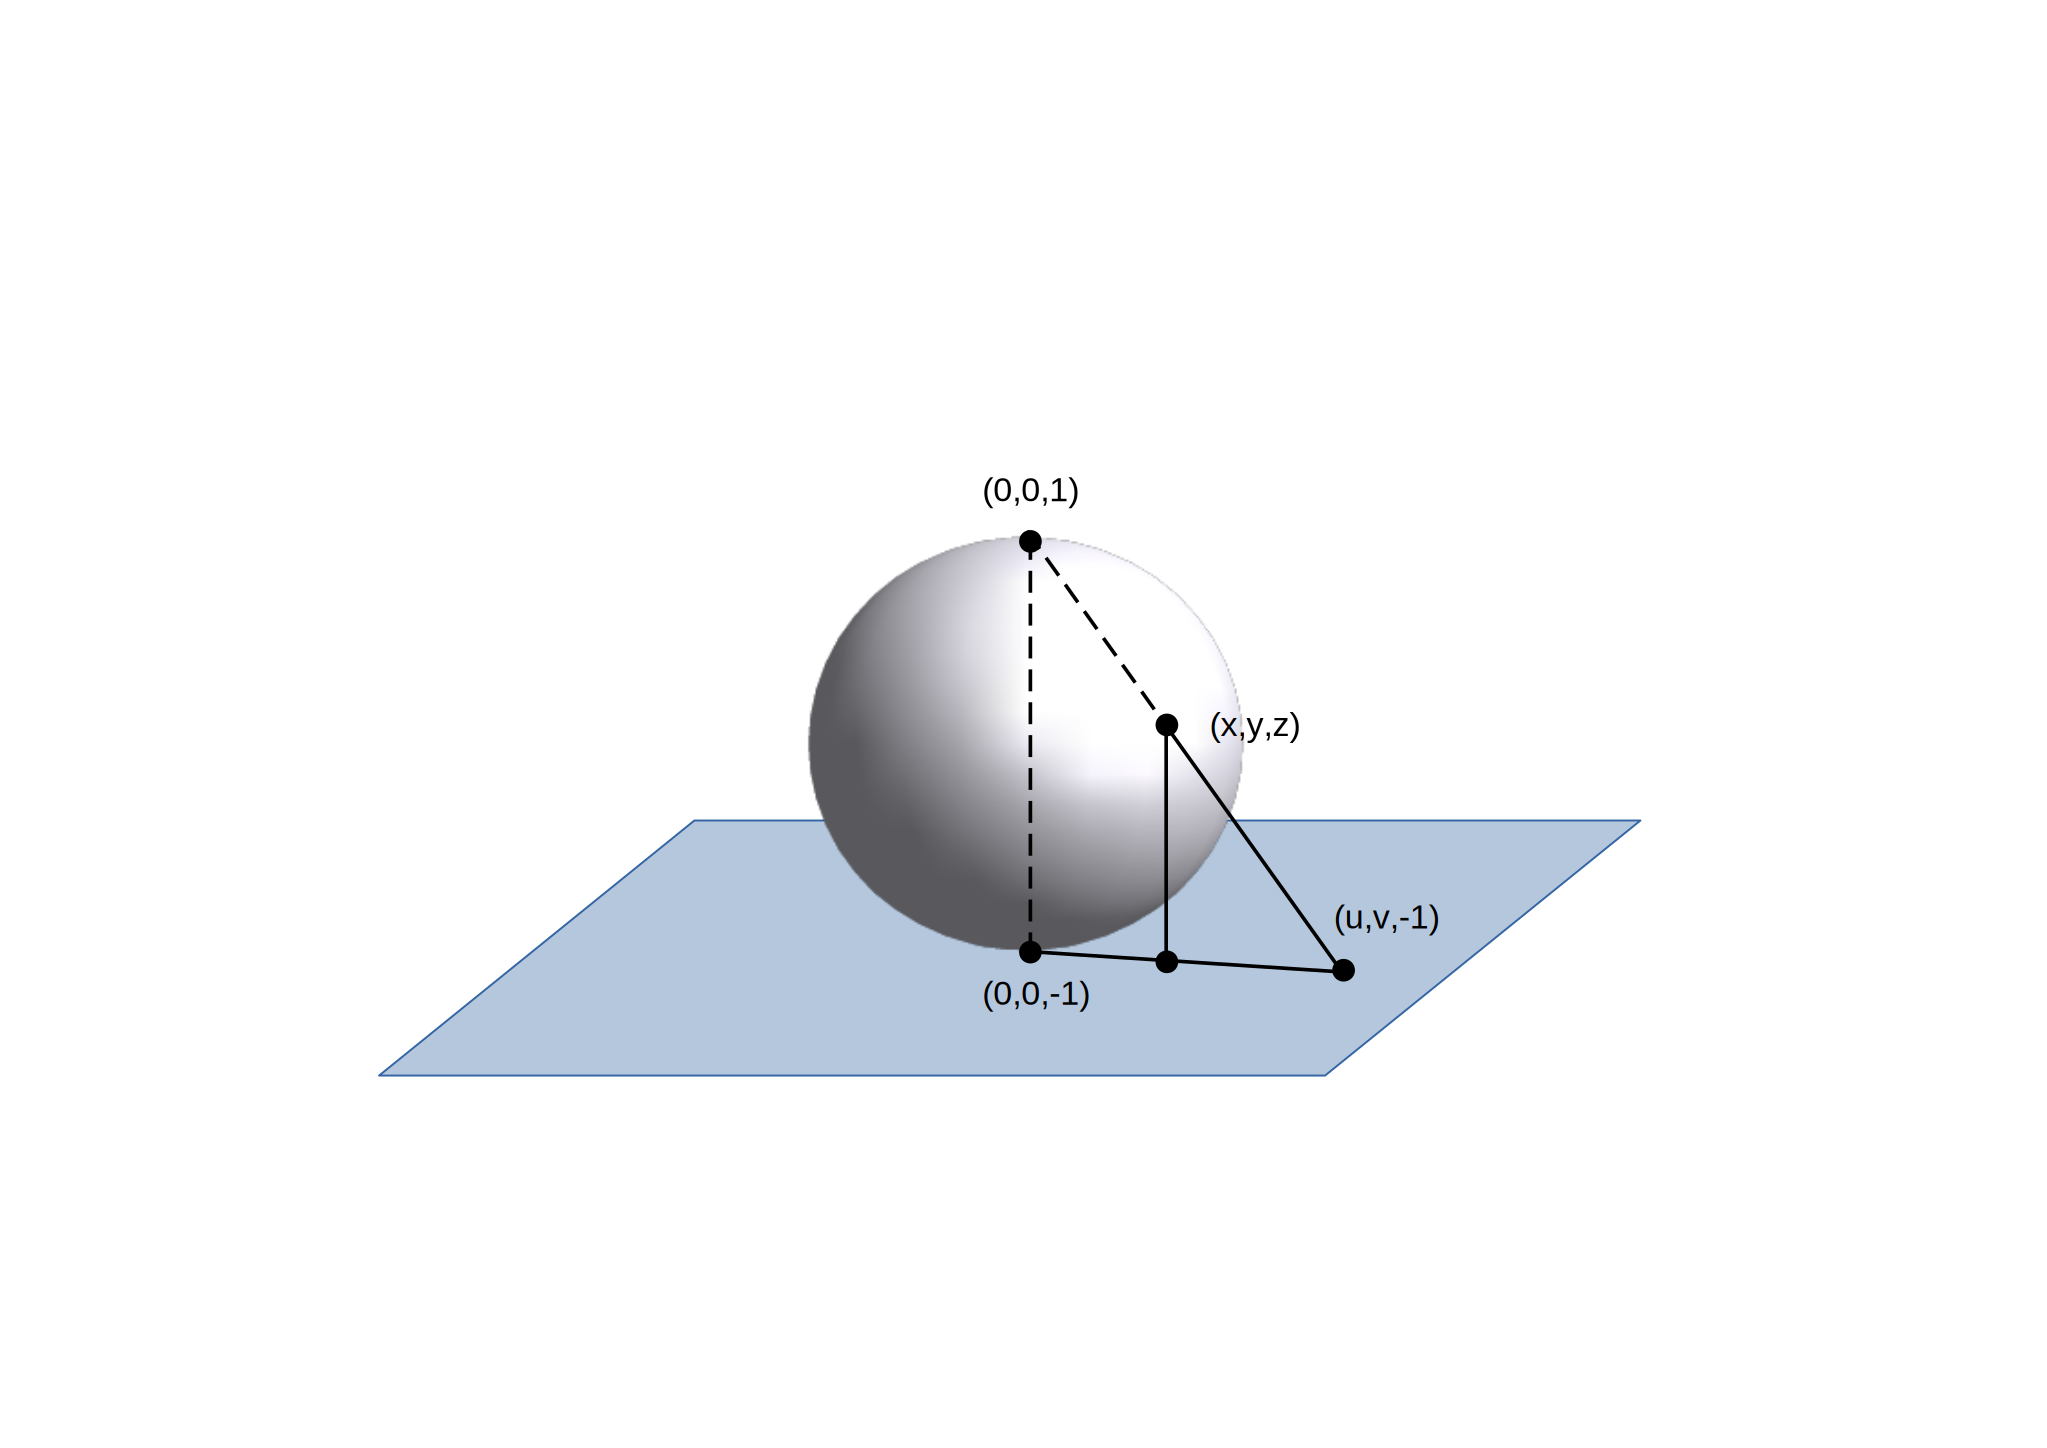
\includegraphics[scale=0.5]{stereo.png}
\end{center}
\caption{Projection stéréographique}
\end{figure}
Pour obtenir un homéomorphisme (i.e. une application bijective continue dont l'inverse est continue) entre $\overline{\C}$ et $\mathbb{S}^2$, il est courant d'avoir recours à une transformation particulière appelée projection stéréographique, qui est également utilisée en géographie pour établir des cartes des régions polaires. Son principe, qui consiste associer de façon univoque un point du plan à un point de la sphère $\mathbb{S}^2$, est résumé en figure \ref{fig:stereo}. Une application immédiate du théorème de Thalès permet d'obtenir les relations suivantes qui définissent la projection:
\begin{equation}
\label{eq:stereo}
x = \frac{2 \mu}{1-\xi} , \, y = \frac{2 \nu}{1-\xi}
\end{equation}
La projection inverse s'obtient tout aussi simplement en utilisant à nouveau Thalès pour obtenir la relation:
\[
x^2 + y^2 = \frac{4}{(1-\xi)^2}\left(\mu^2+\nu^2\right) = \frac{4}{(1-\xi)^2}\left(1-\xi^2\right) = 4 \frac{1+\xi}{1-\xi}
\]
d'où l'on déduit:
\[
\xi = \frac{\left(\frac{r}{2}\right)^2 -1}{\left(\frac{r}{2}\right)^2 +1}, \, r^2 = x^2 + y ^2
\]
puis:
\[
\mu = \frac{x}{\left(\frac{r}{2}\right)^2 +1}, \, \nu = \frac{x}{\left(\frac{r}{2}\right)^2 +1}
\]
En interprétant le plan de projection comme le plan complexe, le point $z = x + i y$ sera transformé en:
\[
\phi(z) = \left(\frac{x}{\left(\frac{|z|}{2}\right)^2 +1}, \frac{y}{\left(\frac{|z|}{2}\right)^2 +1},\frac{\left(\frac{|z|}{2}\right)^2 -1}{\left(\frac{|z|}{2}\right)^2 +1}\right)
\]
En faisant tendre $|z|$ vers $+\infty$ dans l'expression précédente, on remarque que l'on tend vers le point de coordonnées $(0,0,1)$. Ceci permet d'étendre la projection stéréographique inverse à $\overline{\C}$ en posant $\phi(\omega) = (0,0,1)$, établissant ainsi un homéomorphisme entre $\overline{\C}$ et $\mathbb{S}^2$. Du point de vue topologique, ces deux objets sont donc indiscernables. 
\subsection{Connexité}
Intuitivement, une partie connexe est d'un seul tenant: elle ne peut pas être séparée en deux sous-ensembles disjoints à l'aide d'ouverts. Il s'agit d'une notion très fréquemment utilisée dans la théorie des fonctions de la variable complexe. 
\begin{fdefn}
On dira qu'une partie $A$ de $\C$ est connexe s'il n'existe pas deux ouverts $U,V$ de $\C$ tels que $A\cap U \neq \emptyset, A \cap V \neq \emptyset$, $A = (A \cap U) \cup (A \cap V)$ et $(A\cap U)\cap(A \cap V) = \emptyset$.
\end{fdefn}
On montre que cette définition équivaut à la suivante :

\begin{fdefn}
Une partie $A$ de $\C$ est connexe si les seules parties de $A$ à la fois ouvertes et fermées sont $A$ et $\emptyset$
\end{fdefn}

La notion de connexité formalise le fait intuitif d'être d'un seul tenant. Les disques ouverts (resp. fermés) de $\C$ sont des parties connexes. Ceci est la conséquence d'un résultat plus général, donné ci-dessous. 
\begin{fdefn} Un ouvert $U$ de $\C$ est dit \textbf{étoilé} par rapport au point $z_0 \in U$, si pour tout point appartenant à  $U$, le segment de droite joignant $z_0$ à ce point est contenu dans $U$. 
\end{fdefn}


\begin{fprop}
Tout ouvert étoilé de $\C$ est connexe.
\end{fprop}
\begin{proof}
Soit $W$ un ouvert de $\C$ étoilé par rapport au point $z_0$. Supposons qu'il existe deux ouverts $U,V$ tels que $A\cap U \neq \emptyset$, $A \cap V \neq \emptyset$, $U \cap V \cap W = \emptyset$ et $W \subset U \cup V$. Tout point de $W$ appartient donc exclusivement soit à $U$, soit à $V$. Supposons que $z_0 \in U$. Il existe $z_1 \in V \cap W$ et $W$ étant étoilé, le segment: $[z_0,z_1] = \{ (1-t)z_0 + t z_1, \, t \in [0,1]$ appartient à $W$. Soit $\eta = \sup \{ t \in [0,1[ \, \forall u \in [0,t], \,(1-u)z_0 + u z_1 \in U\}$. Si $z_\eta = (1-\eta)z_0 + \eta z_1 \in U$, alors, $U$ étant ouvert, il existe un disque ouvert $D(z_\eta, \epsilon), \epsilon > 0$ inclus dans $U$. Le point $(1-\eta-\epsilon/(2|z_1-z_0|))z_0 + (\eta + \epsilon / (2|z_1-z_0|))z_1$ appartient à $U$, mais aussi à $V$ par définition du $\sup$, ce qui est une contradiction. Le même raisonnement s'applique si $z_\eta \in V$, prouvant ainsi la proposition. 
\end{proof}
La connexité se comporte bien vis-à-vis d'opérations usuelles. En particulier, un produit d'espace connexes est connexe. La proposition suivante est très importante en pratique:
\begin{fprop}
Soit $A$ une partie connexe et $f \colon \C \to \C$ une application continue. Alors la partie $f(A)$ est connexe.
\end{fprop}
\begin{proof}
Supposons l'existence de deux ouverts $U,V$ tels que $f(A)\cap U \neq \emptyset$,$f(A)\cap V \neq \emptyset$, $f(A)\cap U\cap V = \emptyset$ et $f(A) \subset U \cup V$. $f$ étant continue, $f^{-1}(U), f^{-1}(V)$ sont des ouverts tels que: $f^{-1}(U)\cap A \neq \emptyset, f^{-1}(V)\cap A \neq \emptyset$, $f^{-1}(U)\cap f^{-1}(V)\cap A = \emptyset$ et $A \subset f^{-1}(U)\cup f^{-1}(V)$, ce qui est une contradiction, $A$ étant supposée connexe. 
\end{proof}

Enfin, bien que la réunion de parties connexes ne soit généralement pas connexe, ceci est cependant vrai dans le cas où leur intersection n'est pas vide.
\begin{fprop}
\label{prop:union_connexes}
Soit $A_i, i \in I$ une famille quelconque de parties connexes telle que $\bigcap_{i \in I} A _i \neq \emptyset$. Alors $\bigcup_{i \in I} A_i$ est connexe.
\end{fprop}
\begin{proof}
Soient deux ouverts $U,V$ tels que:
\[
U \cap \bigcup_{i \in I} A_i \neq \emptyset, \, V \cap \bigcup_{i \in I} A_i \neq \emptyset, \, U \cap V \cap \bigcup_{i \in I} A_i , \, \bigcup_{i \in I} A_i \subset U \cup V
\]
Soit $x \in \bigcap_{i \in I} A_i$. Par hypothèse $x \in U$ ou $x \in V$. Supposons que $x \in U$ et soit $y \in V \cap \bigcup_{i \in I} A_i $. Il existe $A_k$ tel que: $x \in A_k, \, y \in A_k$. On a donc $U \cap A_k \neq \emptyset, \, V \cap A_k \neq \emptyset$, mais aussi $U \cap V \cap A_k = \emptyset, A_k \subset U \cup V$ ce qui est impossible, $A_k$ étant connexe.
\end{proof}
L'ensemble des parties connexes incluses dans une partie et contenant un point donné vérifie les hypothèses de la proposition précédente. On peut donc parler de plus grande partie connexe contenant un point. Ceci permet d'énoncer le résultat suivant.
\begin{fprop}
Soit $A$ une partie de $\C$. Il existe une partition de $A$ en parties connexes que l'on appelle composantes connexes de $A$.
\end{fprop}
\begin{proof}
Chaque point de $A$ est contenu dans une plus grande partie connexe. En vertu de la proposition \ref{prop:union_connexes}, ces parties sont disjointes car maximales au sens de l'inclusion et forment donc une partition de $A$.
\end{proof}
\begin{rem}
Dans un ouvert $U$ de $\C$, toute composante connexe est ouverte. Soit en effet $x \in U$ et soit $A$ la composante connexe de $U$ le contenant. $U$ étant ouvert, il existe un disque ouvert $D(x,\epsilon)$ contenu dans $U$, mais un disque ouvert étant un ouvert étoilé, il est connexe et est donc inclus dans $A$. On en déduit que $A$ est voisinage de chacun de ses points, donc ouvert.
\end{rem}
\begin{rem}
La remarque précédente montre également que tout ouvert de $\C$ est réunion dénombrable d'ouverts connexes. C'est une conséquence directe de la densité des complexes à coordonnées rationnelles dans $\C$. 
\end{rem}
\subsection{Chemins et connexité par arcs}
\begin{fdefn}
Un chemin de $\C$ est une application continue $\gamma \colon [a,b] \to \C$.
Le point $\gamma(a)$ (resp. $\gamma(b)$) est appelé origine du chemin (resp. extrémité).
\end{fdefn}
\begin{fdefn}
On dira qu'une partie $A$ de $\C$ est connexe par arcs si pour tout couple $(z_0,z_1)$ de points de $A$, il existe un chemin $\gamma \colon [a,b]\to A$ tel que $\gamma(a) = z_0, \gamma(b)=z_1$.
\end{fdefn}
La connexité par arcs est une propriété plus forte que la connexité simple. 
\begin{fprop}
\label{prop:ouvert_connexe}
Toute partie connexe par arcs est connexe et tout ouvert connexe de $\C$ est connexe par arcs. 
\end{fprop}
\begin{proof}
Soit $A$ une partie connexe par arcs et soient $U,V$ deux ouverts de $\C$ tels que $A \cap U \neq \emptyset, A \cap V \neq \emptyset$ et $A \subset U \cup V, A \cap U \cap V = \emptyset$. Soit $z_0 \in U, z_1 \in V$. Par hypothèse, il existe un chemin $\gamma \colon [a,b] \to A$ tel que $\gamma(a) = z_0, \gamma(b)= z_1$. Soit $\eta = \sup \{ t \in [0,1], \gamma([0,t]) \in U\}$. Soit $D(\gamma(\eta),r), r >0$ un disque ouvert contenu dans $U\cup V$. Par continuité de $\gamma$, il existe $\epsilon > 0$ tel que $\gamma(]\eta-\epsilon, \eta +\epsilon[) \subset D(\gamma(\eta),r)$. $D(\gamma(\eta),r)\cap U \neq \emptyset$ car $\gamma([0,t]) \in U$ si $t < \eta$ et $D(\eta,r) \cap V \neq \emptyset$ car par définition du $\sup$, il existe des points de $V$ appartenant à $\gamma([\eta,\eta + \epsilon/2])$. Or $\eta \in U$ ou $\eta \in V$ et $U,V$ sont des ouverts, il devrait donc exister un rayon $r^\prime > 0$ tel que $D(\gamma(\eta),r^\prime)\subset U$ ou $D(\gamma(\eta),r^\prime)\subset V$, ce qui est contradictoire. 

La seconde partie de la proposition, que l'on peut voir comme une réciproque partielle, utilise un très important argument basé sur la connexité simple que l'on retrouvera un peu plus loin dans le cours. Soit $U$ un ouvert connexe de $\C$ et $z_0$ un point de $U$. L'ensemble $A=\{ z \in U , \, \exists \gamma \colon [a,b] \to U, \gamma(a)=z_0, \gamma(b) = z\}$ est un ouvert. En effet, soit $z \in A$. $U$ étant ouvert, il existe $D(z, \epsilon), \epsilon > 0$ tel que $D(z,\epsilon) \subset U$. Soit $u \in D(z,\epsilon)$. Par hypothèse, il existe un chemin $\gamma$ d'origine $z_0$ et d'extrémité $z$. D'autre par, le segment $[z,u]$ appartient à $D(z, \epsilon)$, donc à $U$ et le chemin obtenu concaténant $\gamma$ avec $[z,u]$ est continu, d'où $u \in A$. $U-A$ est également un ouvert. En effet, soit $z \in U-A$.Il existe $\epsilon > 0$ tel que $D(z,\epsilon) \subset U$. $D(z,\epsilon)$ ne peut contenir aucun point de $A$ sans quoi il existerait un chemin joignant $z_0$ à $z$. On a donc $D(z,\epsilon) \subset U-A$. Les ouverts $A,U-A$ sont disjoints, d'union $U$. Comme $A$ n'est pas vide car contenant au moins $z_0$, on doit avoir $U-A=\emptyset$ par connexité de $U$, ce qui termine la démonstration.
\end{proof}
La connexité par arcs est préservée par les applications continues.
\begin{fprop}
Soit $A \subset \C$ une partie connexe par arcs et $f \colon \C \to \C$ une application continue. Alors $f(A)$ est connexe par arcs.
\end{fprop}
\begin{proof}
Soient $z_0,z_1 \in f(A)$. Il existe $p,q \in A$ tels que $f(p) =z_0, f(q)=z_1$. $A$ étant connexe par arcs, il existe $\gamma \colon [a,b] \to A$ tel que $\gamma(a) = p, \gamma(b) = q$. L'application $f \circ \gamma$ est un chemin reliant $z_0,z_1$, prouvant ainsi la connexité par arcs de $f(A)$.
\end{proof}
\begin{exercice}
    Montrer que $\C$ et $\R$ ne sont pas homéomorphes. 
    
    \textbf{Indication:} Montrer que si $\phi \colon \C \to \R$ est un homéomorphisme, alors $\Phi\left(\C-\{0\}\right)$ n'est pas connexe.    
\end{exercice}
\begin{fdefn} Un sous ensemble $\Omega$ du plan complexe est un \textbf{domaine} si $\Omega$ est un ouvert non vide connexe. 
\end{fdefn}
\begin{rem}
En vertu de la proposition \ref{prop:ouvert_connexe}, il équivalent de vérifier que $\Omega$ est connexe par arcs, ce qui est souvent plus simple.
\end{rem}

Un disque ouvert de rayon non nul est un domaine, de même qu'une couronne ouverte définie comme:
\[
\mathcal{C}(z;r_1,r2) =  \{ z : 0<r_1 <\lvert z-z_0 \rvert <r_2\}. 
 \]
 Tout ouvert étoilé non vide est un domaine.


\begin{figure}[H]
\begin{center}
\shorthandoff{!}\shorthandoff{:}
\begin{tikzpicture}
\clip(-3,-3) rectangle (10,3);
\begin{scope}[xshift=7 cm]
 \tikzstyle{point}=[circle,thick,draw=black,fill=black,inner sep=0pt,minimum width=4pt,minimum height=4pt]
    \fill[color=gray!40] (-2,0) -- (-1,0.5) -- (0,2) -- (1,0.5) -- (2,0) -- (1,-0.5) -- (0,-2) -- (-1,-0.5) -- cycle;
    \node (a)[point,label=$z_0$] at (0,0) {};
\end{scope}
\fill[color=gray!40,even odd rule] (0,0) circle(1) circle(2);
\end{tikzpicture}
\shorthandon{!}\shorthandoff{:}
\caption{Exemples de domaines : anneau et ouvert étoilé par rapport à $z_0$. Notons que l'anneau n'est étoilé par rapport à aucun de ses points.}\label{fig:domaines}
\end{center}
\end{figure}
 Dans la suite, nous désignerons par $U$ les ouverts de $\C$ et par $\Omega$ les domaines de $\C$. Les domaines joueront un rôle important dans la théorie de l'intégration d'une fonction de la variable complexe le long d'un chemin.



\begin{fdefn}
Soit $U$ un ouvert de $\C$. Un chemin de classe $C^k$ par morceaux dans $U$ est une application continue $\gamma$ d'un intervalle réel $[a,b]$ dans $U$ telle qu'il existe une subdivision $a=t_0 < t_1 < \dots < t_N = b$ pour laquelle $\gamma$ est de classe $C^k$ sur chaque intervalle $]t_i,t_{i+1}[, \, i=0 \dots N$. Nous dirons que $\gamma$ est un chemin joignant les points $\gamma(a)$ (l'origine) et $\gamma(b)$ (l'extrémité) dans $U$.
\end{fdefn}
Dans toute la suite, le terme \og chemin \fg{} désignera de façon implicite un chemin de classe $C^k$ par morceaux, l'indice de régularité $k$ étant précisé lorsque cela est nécessaire. 

L'ensemble image $\lvert\gamma \rvert:=\gamma([a, b])\subset U$ est appelé \emph{trace} du chemin. Comme $\gamma$ est continue, $\lvert\gamma \rvert$ est un ensemble compact. Il convient de noter qu'un chemin est plus que sa simple trace ; cette dernière étant traversée selon la loi $\gamma(t)$. En particulier :

\begin{fdefn}
Soit $\gamma \colon [a,b] \to U$ un chemin. Soit $\phi \colon [c,d] \to [a,b]$ un difféomorphisme de classe $C^k$. Le chemin $\gamma \circ \phi$ sera dit obtenu à partir de $\gamma$ par changement de paramètre. Un changement de paramètre $\phi$ strictement croissant sera dit préservant l'orientation.
\end{fdefn}
La trace d'un chemin obtenu par changement de paramètre est semblable à celle du chemin initial. Son sens de parcours n'est pas modifié si le changement de paramètre préserve l'orientation. Dans toute la suite, les grandeurs associées aux chemins seront invariantes par changement de paramètre préservant l'orientation: on pourra donc choisir de façon arbitraire l'intervalle de définition d'un chemin de telle sorte que les calculs soient les plus simples possible. Pour les définitions qui vont suivre, on se placera sur l'intervalle $[0,1]$ afin d'alléger les écritures. Nous utiliserons également la notation $\gamma$ pour définir le chemin et sa trace.


\begin{exem}
\begin{enumerate}
\item Un chemin $\gamma$ est appelé chemin \textbf{nul}, si la fonction $\gamma$ est constante. La trace est alors constituée d'un seul point. Un tel chemin est continument différentiable.
\item Le segment $[z_0, z_1]$ est le chemin continument différentiable défini par
\[\gamma(t) := (1 - t)z_0 + tz_l, \quad t \in [0,1].\]
\item Soit $c \in \C$, et $r > 0$. La fonction 
\[\gamma(t) := c + r e^{it}, \quad t \in [a,b],\]
avec $0 \leq a < b \leq 2 \pi$ est continument différentiable. Le chemin $\gamma$ correspondant est un arc circulaire situé sur la frontière du disque $B(c;r)$. Lorsque $a=0$ et $b=2 \pi$, le chemin $\gamma$ est le cercle centré en $c$ et de rayon $r$.  
\end{enumerate}
\end{exem}



\begin{fdefn}
Un chemin $\gamma$ est dit \textbf{simple} si $\gamma(s) \neq \gamma(t)$ quand $s\neq t$. Un chemin est appelé \textbf{lacet} si son origine coïncide avec son extrémité, donc si $\gamma(0)=\gamma(1)$. Un \textbf{lacet simple} est un lacet tel que $ \gamma(s)\neq \gamma(t)$ pour $0 \leq s<t<1$. 
\end{fdefn}


\begin{figure}[H]
\begin{center}
\shorthandoff{!}\shorthandoff{:}
\begin{tikzpicture}
\tikzset{
    on each segment/.style={
        decorate,
        decoration={
            show path construction,
            moveto code={},
            lineto code={
                \path [#1]
                (\tikzinputsegmentfirst) -- (\tikzinputsegmentlast);
            },
            curveto code={
                \path [#1] (\tikzinputsegmentfirst)
                .. controls
                (\tikzinputsegmentsupporta) and (\tikzinputsegmentsupportb)
                ..
                (\tikzinputsegmentlast);
            },
            closepath code={
                \path [#1]
                (\tikzinputsegmentfirst) -- (\tikzinputsegmentlast);
            },
        },
    },
}
    \begin{scope}[scale=2]
        \node[label=below:$A$] (A) at (0,0) {};
        \node[label=below:$B$] (B) at (2,0.25){};
        \draw[blue] plot [smooth,tension=1]
        coordinates {(A) (1,0) (1.14,-0.6) (0.5,-0.5) (0.5,0.5) (1.5,0) (B)}[postaction={on each segment={draw,-{stealth[red,bend]}}}];
        \draw (1, -1) node {chemin quelconque};
        \draw [fill=black] (A) circle (1pt);
    \draw [fill=black] (B) circle (1pt);
    \end{scope}
    \begin{scope}[scale=2,xshift= 3 cm]
        \node[label=below:$A$] (A) at (0,0) {};
        \node[label=below:$B$] (B) at (2,0.25){};
        \draw[blue] plot [smooth,tension=1]
        coordinates {(A)  (0.5,0.5) (1.5,0) (B)}[postaction={on each segment={draw,-{stealth[red,bend]}}}];
        \draw (1, -1) node {chemin simple};
        \draw [fill=black] (A) circle (1pt);
    \draw [fill=black] (B) circle (1pt);
    \end{scope}
\begin{scope}[scale=2,xshift= 6 cm]
        \node[label=below:$A$] (A) at (0,0) {};
       % \node[label=below:$B$] (B) at (2,0.25){};
        \draw[blue] plot [smooth,tension=1]
        coordinates {(A)  (0.5,0.5) (1.5,0.25) (1.5,-0.25) (0.5,-0.5) (A)}[postaction={on each segment={draw,-{stealth[red,bend]}}}];
        \draw (1, -1) node {lacet simple};
        \draw [fill=black] (A) circle (1pt);
   
    \end{scope}    
    
    
\end{tikzpicture}

\shorthandon{!}\shorthandoff{:}

\end{center}
\end{figure}



\begin{fdefn}
Soient $\gamma_1, \gamma_2$ deux chemins de $[0,1]$ dans un ouvert $U$ de $\C$ tels que $\gamma_1(1) =
\gamma_2(0)$. Le chemin $\gamma_2 + \gamma_1$, somme de $\gamma_1$ et
$\gamma_2$, est défini par :
\[(\gamma_2 + \gamma_1)(t) = \left \{
\begin{array}{cc}
\gamma_1(2t) & \text{ si } t \in \left[0,\frac{1}{2}\right] \\
\gamma_2(2t-1) & \text{ si } t \in \left]\frac{1}{2},1\right]
\end{array}
\right.
\]
\end{fdefn}

Le chemin $\gamma_1 + \gamma_2 + \cdots + \gamma_n$ somme d'un nombre fini des chemins $\gamma_1,\gamma_2,\cdots, \gamma_n$ (dont les origines et extrémités sont appropriées) est défini de la même façon. On vérifie que la somme des chemins est une opération associative, elle n'est pas commutative. Notons qu'il est toujours possible d'écrire de décomposer un chemin $C^k$ par morceaux en une somme de chemins $C^k$. 


\begin{fdefn}
Soit $\gamma$ un chemin de $[0,1]$ dans un ouvert $U$ de $\C$. Le chemin opposé, noté
$-\gamma$, est défini par:
\[(-\gamma)(t) = \gamma(1-t), \quad t \in [0,1]
\]
\end{fdefn}
Le chemin opposé est obtenu par le changement de paramètre $\phi(t)=1-t$ qui ne préserve pas l'orientation. Le chemin opposé possède donc la même image, mais est \og parcouru dans la direction opposée \fg{}.
Les opérations sur les chemins sont résumées figure \ref{ch8:fig1}.
%\begin{figure}[ht]
%\includegraphics[scale=0.4]{images/chemins.pdf}
%\caption{Chemins composé et inverse}\label{ch8:fig1}
%\end{figure}
\begin{figure}[ht]
\begin{center}
\shorthandoff{!}\shorthandoff{:}
\begin{tikzpicture}
\tikzset{
    on each segment/.style={
        decorate,
        decoration={
            show path construction,
            moveto code={},
            lineto code={
                \path [#1]
                (\tikzinputsegmentfirst) -- (\tikzinputsegmentlast);
            },
            curveto code={
                \path [#1] (\tikzinputsegmentfirst)
                .. controls
                (\tikzinputsegmentsupporta) and (\tikzinputsegmentsupportb)
                ..
                (\tikzinputsegmentlast);
            },
            closepath code={
                \path [#1]
                (\tikzinputsegmentfirst) -- (\tikzinputsegmentlast);
            },
        },
    },
}
    
     
    
  \begin{scope}[scale=2]
        \node[label=below:$\gamma(0)$] (A) at (0,0) {};
        \node[label=above:$\gamma(1)$] (B) at (2,0.25){};
        \draw[blue] plot [smooth,tension=1]
        coordinates {(A)  (0.5,0.5) (1.5,0) (B)}[postaction={on each segment={draw,-{stealth[red,bend]}}}];
       \draw [fill=black] (A) circle (1pt);
    \draw [fill=black] (B) circle (1pt);
  \end{scope}    
    
  \begin{scope}[scale=2, yshift=-1cm]     
      \node[label=below:$-\gamma(1)$] (A) at (0,0) {};
        \node[label=above:$-\gamma(0)$] (B) at (2,0.25){};
        \draw[blue] plot [smooth,tension=1]  
    coordinates {(B)  (1.5,0) (0.5,0.5)  (A)}[postaction={on each segment={draw,-{stealth[red,bend]}}}];
       \draw [fill=black] (A) circle (1pt);
    \draw [fill=black] (B) circle (1pt);    
    \end{scope}
  
  \begin{scope}[scale=2, xshift = 3cm]
        \node[label=below:$\gamma_1(0)$] (A) at (0,0) {};
        \node[label=above:{$\gamma_1(1)=\gamma_2(0)$}] (B) at (2,0.25){};
        \draw[blue] plot [smooth,tension=1]
        coordinates {(A)  (0.5,0.5) (1.5,0) (B)}[postaction={on each segment={draw,-{stealth[red,bend]}}}];
       \draw [fill=black] (A) circle (1pt);
    \draw [fill=black] (B) circle (1pt);
       \node[label=below:$\gamma_2(1)$] (C) at (3.5,0.25){};
        \draw[blue] plot [smooth,tension=1]
       coordinates {(B)  (2.5,-0.5) (3,0) (C)}[postaction={on each segment={draw,-{stealth[red,bend]}}}];
      \draw [fill=black] (C) circle (1pt);
   \end{scope}     
    
        
\end{tikzpicture}

\shorthandon{!}\shorthandoff{:}
\caption{Chemins inverse et composé.}\label{ch8:fig1}
\end{center}
\end{figure}


Il est possible de définir la longueur d'un chemin en l'approchant par des chemins polygonaux: c'est Archimède qui semble-t-il est le premier à avoir eu cette idée. La proposition suivante résume ce procédé.
\begin{fprop}
Soit $\gamma \colon [a,b] \to \C$ un chemin de classe $C^k$, $k \geq 1$. Pour toute subdivision $\mathcal{S} = \{a=t_0 < t_1 \dots < t_n = b\}$ de l'intervalle $[a,b]$, on pose :
\[
l(\mathcal{S}) = \sum_{i=0}^{n-1} \lvert \gamma(t_{i+1}) - \gamma(t_i) \rvert.
\]
La borne supérieure de l'ensemble $\{l(\mathcal{S})\}$ où $\mathcal{S}$ parcourt les subdivisions de $[a,b]$ est finie et vaut :
\[
l(\gamma) = \int_a^b \lvert\gamma^\prime(t)\rvert \diff t.
\]
la valeur $l(\gamma)$ est appelée longueur du chemin $\gamma$.
\end{fprop}
\begin{proof}
On remarque tout d'abord, en vertu du théorème des accroissements finis que :
\[
\lvert \gamma(t_{i+1}) - \gamma(t_i) \rvert  = \left\lvert \int_{t_i}^{t_{i+1}} \gamma^\prime(s) \diff s \right\rvert \leq \int_{t_i}^{t_{i+1}}\left\lvert \gamma^\prime(s) \right\rvert\diff s .\]
On en déduit que pour toute subdivision $\mathcal{S}$ :
\[
l(\mathcal{S}) \leq  \int_a^b \left\lvert \gamma^\prime(s) \right\rvert \diff s,\]
et par conséquent la borne supérieure de l'ensemble $\{l(\mathcal{S})\}$ où $\mathcal{S}$ parcourt les subdivisions de $[a,b]$ est donc finie. Soit maintenant $\epsilon > 0$, l'application $\gamma$ étant de classe $C^1$, sa dérivée est continue sur le compact $[a,b]$, donc uniformément continue. Il existe donc $\eta>0$, telle que pour toute subdivision $\mathcal{S} = \{a=t_0 < t_1 \dots < t_n = b\}$  dont le pas, $\delta :=\sup_{i=0}^{n-1}(t_{i+1}-t_i)$, est tel que $\delta<\eta$, on ait, pour tout $i=0, \cdots, n-1$, l'inégalité 
\[
\lvert \gamma^\prime(s) - \gamma^\prime(t_i)\rvert < \epsilon, \quad s \in [t_i, t_{i+1}].
\]
Ceci implique que pour tout $i=0,\dots,n-1$:
\begin{align*}
\Bigl \lvert\int_{t_i}^{t_{i+1}} (\gamma^\prime(s) - \gamma^\prime(t_i)) \diff s \Bigr \rvert & = \lvert \gamma(t_{i+1}) - \gamma(t_i) - \gamma^\prime(t_i) (t_{i+1}- t_i) \rvert \\& < \epsilon (t_{i+1}-t_i),
\end{align*}
soit finalement :
\[
\Bigl \lvert \lvert\gamma(t_{i+1}) - \gamma(t_i)\rvert -  \lvert\gamma^\prime(t_i) \rvert(t_{i+1}-t_i)\Bigr \rvert < \epsilon (t_{i+1}-t_i).
\]
On en déduit par sommation sur $i$ et application de l'inégalité triangulaire :
\[
\Bigl \lvert l(S) - \sum_{i=0}^n  \lvert\gamma^\prime(t_i) \rvert(t_{i+1}-t_i)\Bigr \rvert < \epsilon (b-a).
\]
Par une propriété connue des intégrales de Riemann, il existe un $\eta^\prime$ tel que si $\delta< \eta^\prime$, alors :  
\[
\Bigl  \lvert \int_a^b \lvert\gamma^\prime(s)\rvert ds -  \sum_{i=0}^n  \lvert\gamma^\prime(t_i) \rvert(t_{i+1}-t_i) \Bigr \rvert  < \epsilon .\]
En choisissant $\eta_0=\min (\eta, \eta^\prime)$, pour toute subdivision de pas $\delta<\eta_0$, 
\[ \Bigl \lvert l(\mathcal{S}) - \int_a^b \lvert\gamma^\prime(s)\rvert \diff s \Bigr \rvert < \epsilon(1 + (b-a)),\]
ce qui termine la preuve.
\end{proof}
Lorsque le chemin est de classe $C^k$ par morceaux, on définit sa longueur par sommation. 
\begin{fdefn}
Soit $\gamma \colon [a,b] \to \C$ un chemin de classe $C^k$ sur chacun des intervalles $]t_i,t_{i+1}[$, où $\{a=t_0 < t_1 \dots < t_n = b\})$ est une subdivision de l'intervalle $[a,b]$. Sa longueur est définie par:
\[
l(\gamma) = \sum_{i=0}^{n-1} \int_{t_i}^{t_{i+1}} \lvert \gamma^\prime(t) \rvert \diff t
\]
\end{fdefn}
La proposition suivante établit le fait que la longueur d'un chemin est un invariant géométrique qui ne dépend que de sa trace et non de sa paramétrisation. Cette proposition se prouve en utilisant la formule du changement de variable dans les intégrales. 
\begin{fprop}
La longueur d'un chemin de classe $C^k$ par morceaux est invariante par changement de paramétrage.
\end{fprop}
\begin{rem}
Le procédé d'approximation par des chemins polygonaux permet de définir la longueur de chemins simplement continus, mais celle-ci peut être infinie. C'est par exemple le cas de courbe fractale comme la courbe de Koch. Cette dernière s'obtient à partir d'un segment de droite en modifiant récursivement chaque segment de droite de la façon suivante : 
1) on divise le segment de droite en trois segments de longueurs égales, 2) on construit un triangle équilatéral ayant pour base le segment médian de la première étape, 3) on supprime la base du triangle de la deuxième étape (cf. figure~\ref{fig:Koch}). On peut montrer qu'à l'étape $n$, la longueur de la courbe obtenue est supérieure à $(4/3)^n$. Lorsque la longueur d'un chemin est finie, on dit que le chemin est \textbf{rectifiable}. L'absence de formule de calcul utilisable dans le cas général fait qu'en pratique, on se restreint aux chemins de classe $C^k$ par morceaux.
\begin{figure}[ht]
\includegraphics[scale=0.8]{courbe_Koch}
\caption{Courbe de Von Koch : les quatre premières étapes}\label{fig:Koch}
\end{figure}
 
\end{rem}
\section{Exercice complémentaire}
\begin{exer}[\textbf{Projection stéréographique}]
Le but de cet exercice est d'établir une formule explicite connectant le point $z = x +i y \in \C$ et sa projection $\hat{z}$ sur $\Sigma$. Soit $(X,Y,Z)$ les coordonnées cartésiennes de $\hat{z}$, où l'axe $Z$ passe par $N$ et les axes $X$ et $Y$ coïncident avec les axes $x,y$ de $\C$.  Soit $z' = X+i Y$ le pied de la perpendiculaire à $\C$ passant par $\hat{z}$. 

\begin{figure}[ht]
\begin{center}
\shorthandoff{!}\shorthandoff{:}
\begin{tikzpicture}[line cap=round,line join=round,>=triangle 45,x=9.999999999999998cm,y=10.0cm, scale=0.3]
\clip(-1.0204444716563346,-1.1991274885913612) rectangle (2.500817665540407,1.2986943169702587);
\draw[fill opacity=0.10000000149011612] (0.055454528631341884,0.6249841873023777) -- (0.05545452863134189,0.6804387159337196) -- (0.,0.6804387159337196) -- (0.,0.6249841873023777) -- cycle; 
\draw[fill opacity=0.10000000149011612] (0.055454528631341884,0.) -- (0.05545452863134189,0.05545452863134188) -- (0.,0.055454528631341884) -- (0.,0.) -- cycle; 
\draw[fill opacity=0.10000000149011612] (0.8360919384587128,0.) -- (0.8360919384587128,0.05545452863134188) -- (0.7806374098273708,0.055454528631341884) -- (0.7806374098273708,0.) -- cycle; 
\draw(0.,0.) circle (10.cm);
\draw (0.,1.)-- (2.081611983804011,0.);
\draw (0.,0.)-- (0.7806374098273708,0.6249841873023777);
\draw (0.5519676853769542,-0.8697443933524662) node[anchor=north west] {$\Sigma$};
\draw (-0.09895605045228752,-0.010995609336775847) node[anchor=north west] {$O$};
\draw (-0.11464095974937767,1.1849787245663546) node[anchor=north west] {$N$};
\draw (0.8225323707517594,0.7850135374905536) node[anchor=north west] {$\hat{z}$};
\draw (2.0930100238160625,0.13016857433703627) node[anchor=north west] {$z$};
\draw [line width=0.4pt] (0.,0.6249841873023777)-- (0.7806374098273708,0.6249841873023777);
\draw [line width=0.4pt] (0.7806374098273708,0.6249841873023777)-- (0.7806374098273708,0.);
\draw (0.7558715062391264,-0.003153154688230729) node[anchor=north west] {$z'$};
\draw (0.573525732429403,0.38112712309048) node[anchor=north west] {$Z$};
\draw (-0.14993200566783055,0.5732672619798354) node[anchor=north west] {$1$};
\draw [domain=-1.0204444716563346:2.500817665540407] plot(\x,{(-0.-0.*\x)/-2.081611983804011});
\draw (0.,1.)-- (0.,0.);
\begin{scriptsize}
\fill [color=pblue] (0.,0.) circle (5pt);
\fill [color=pblue] (0.,1.) circle (5pt);
\fill [color=pblue] (0.7806374098273708,0.6249841873023777) circle (5pt);
\fill [color=pblue] (2.081611983804011,0.) circle (5pt);
\fill [fill=pblue] (0.,0.6249841873023777) circle (5pt);
\fill [color=pblue] (0.7806374098273708,0.) circle (5pt);
\end{scriptsize}
\end{tikzpicture}

\shorthandon{!}\shorthandoff{:}
\caption{Projection stéréographique}\label{fig8}
\end{center}
\end{figure}

Alors $z'$ et $z$ sont dans la même direction, ainsi
\[z=\frac{\lvert z \rvert}{\lvert z' \rvert} z'.\]
\begin{MYenumerate}
\item En observant la figure~\ref{fig8}, qui représente la section verticale de la sphère et de $\C$ passant par $N$ et $\hat{z}$, que les triangles rectangles d'hypoténuse $N \hat{z}$ et $Nz$ sont semblables, en déduire que 
\[\frac{\lvert z \rvert}{\lvert z' \rvert} = \frac{1}{1-Z}.\]
\item Obtenir la première formule
\[x+iy = \frac{X+i Y}{1-Z},\]
puis l'inverser pour trouver les coordonnées de $\hat{z}$ en fonction des coordonnées de $z$.
\item Une cercle sur $\Sigma$ passant par le point $N=(0,0,1)$ est l'intersection du plan d'équation $a X + b Y +c(Z-1)=0$ avec $\Sigma$. En déduire que les images $z$ vérifient une équation de la forme
\[\bar{\alpha} z + \alpha \bar{z}=k \]
avec $\alpha  \in \C^\ast$ et $k \in \R$ que l'on exprimera en fonction des constantes réelles $a,b,c$. Montrer que l'on obtient l'équation d'une droite dans $\C$.
\item Si le cercle ne passe pas par $N$, en raison de la symétrie de la sphère, une simple rotation permet de considérer le cercle comme l'intersection du plan $Z=k$ avec $\Sigma$ (avec $k>0$). Montrer alors que $\lvert z\rvert ^2$ est constant et donc que l'image est un cercle centré à l'origine.  
\end{MYenumerate}
Il existe des démonstrations purement géométriques de ces résultats, par exemple dans l'excellent livre \cite{hilbert1983geometry}.
\end{exer}
%%%%%%%%%%%%%%%%%%%%%%%%%%%%%%%%%%%%%%%%%%%%
%%%%%%%%%%%%%%%%%%%%%%%%%%%%%%%%
\chapter{Holomorphie}
La notion de dérivée d'une fonction dans le plan complexe est définie dans ce chapitre. Il sera montré plus loin qu'une application différentiable dans $\C$ possède des propriétés très particulières.

\section{Fonction d'une variable complexe}
Une fonction d'une variable complexe se définit de manière assez similaire à une fonction d'une variable réelle. Si $D$ est un domaine de $\C$, une fonction $f$ sur $D$ assigne à chaque $z \in D$ un nombre complexe $w$ appelé image de $z$ par $f$. On peut écrire $w = f(z) = u+iv$

\section{Rappels de calcul différentiel}

\subsection{Différentiabilité d'une application entre deux espaces vectoriels}

De façon générale, la différentiabilité en un point $x_0$ d'une application $f$ entre espaces vectoriels normés se traduit par l'existence d'un modèle affine continu approchant $f$ au voisinage de $x_0$.
\begin{defn}
Soient $E,F$ deux espaces vectoriels normés et soit $x_0$ un point de $E$. On dira que deux couples $(U,f),(V,g)$, avec $U,V$ voisinages ouverts de $x_0$ et $f\colon U \to F$,$g \colon V \to F$ applications continues, ont même germe en $x_0$ si et seulement si il existe un ouvert $W \subset U \cap V$ tel que $f\rvert_{W}=g\rvert_{W}$.
\end{defn}
\begin{prop}
La relation $(U,f) \sim_{x_0} (V,g)$ si et seulement si les deux couples ont même germe en $x_0$ est une relation d'équivalence. L'ensemble quotient $\{(U,f)\} / \sim_{x_0}$ est appelé ensemble des germes d'applications continues en $x_0$ à valeurs dans $F$ 
\end{prop}
\begin{defn}
Soit $E$ un espace vectoriel normé et $x_0$ un point de $E$. Soit $(U,g)$ un germe d'application continue en $x_0$ à valeurs dans $\R^+$ . On dira qu'un germe en $x_0$ $(V,f)$ à valeurs dans $F$, espace vectoriel normé,  est négligeable devant $(U,g)$ si pour tout $\epsilon > 0$, il existe un voisinage ouvert $W$ de $x_0$ inclus dans $U\cap V$ et tel que:
\[
\forall x \in W, \, \|f(x)\| < \epsilon g(x)
\]
L'ensemble des germes négligeables devant $(U,g)$ est noté $o_{x_0}(g)$.
\end{defn}
\begin{rem}
Il est important de bien prendre garde au fait que la notation $o$ désigne en réalité un ensemble de germes d'applications. On omet le plus souvent l'ouvert $U$ qui est implicite. \end{rem}
\begin{fdefn}
Soient $E,F$ deux espaces vectoriels normés sur un corps $\mathbb{K}$
 et soit $U$ un ouvert de $E$. On dira que $f \colon U \to F$ est différentiable en $x_0 \in U$ si il existe une application continue $L \colon E \to F$ et un voisinage ouvert $V$ de $x_0$ tels que:
 \[
 \forall x \in U \cap V, \, f(x) = f(x_0) + L(x-x_0) + o(\|x-x_0\|_E)
 \]
\end{fdefn}
\begin{rem}
La continuité de $L$ n'est pas une conséquence de la linéarité comme en dimension finie. 
\end{rem}
L'application $ x \mapsto f(x_0) + L(x-x_0)$ est appelée application affine tangente à $f$ en $x_0$.
\begin{prop}
Lorsqu'elle existe, l'application linéaire $L$ est unique.
\end{prop}
\begin{proof}
Supposons l'existence de deux applications linéaires  $L_1, L_2$ vérifiant la relation de définition. On pose $L =  L_1 - L_2$.Pour tout $\epsilon > 0$, il existe un ouvert $W \subset U \cap V$ tel que:
\[
\forall x \in W, \|L(x-x_0)\|_F < \epsilon \| x-x_0 \|_E
\]
Par linéarité, ceci implique:
\[
\forall v \in F, \|v\|_E = 1 \Rightarrow \|L v \|_F < \epsilon 
\]
et donc par passage à la limite:
\[
\forall v \in F, \|v\|_E = 1 \Rightarrow \|L v \|_F = 0
\]
prouvant ainsi que $L$ est l'application nulle.
\end{proof}
\subsection{Différentiabilité d'une application de $\R^2$ dans $\R^2$}
\begin{fdefn}\label{def:1.2}
Soit $U \subset \R^2$ un ouvert et soit une application $f \colon U \to \R^2$.
On dira que $f$ est différentiable en $z_0 \in U$ si il existe une application $\R$-linéaire $ L \colon \R^2 \to \R^2$ telle que :
\[f(z)=f(z_0) + L(z-z_0) + o(\|z-z_0\|_E),\]
\end{fdefn}


%On a nécessairement $A(x_0)=f(x_0)$. En effet, par définition de l'ensemble $o(\|x-x_0\|)$, il existe un voisinage $U$ de $x_0$ tel que:
%\[
%\forall x \in U, \, \|f(x)-A(x)\| \leq \|x-x_0\|
%\]
%et la propriété s'ensuit en prenant $x=x_0$.



%On fait le plus souvent l'abus de notation consistant à confondre \textbf{l'ensemble} $ o(\|x-x_0\|)$ avec un de ses éléments, pour écrire la relation entre $f$ et $H$  au voisinage de $x_0$ sous la forme:
%\[
%f(x) = f(x_0) + H(x-x_0) + o(\|x-x_0\|)
%\]
%Cette notation est la plus courante, mais se révèle parfois source d'erreurs: il faut toujours garder à l'esprit
%que le terme $o(\|x-x_0\|)$ est en fait une \textbf{fonction} négligeable devant $\|x-x_0\|$ au voisinage de $x_0$.
On notera le plus souvent $L$ par $Df(z_0)$ ou $f^\prime(z_0)$ ; il faut garder à l'esprit que ces notations désignent des applications linéaires.
%
%Lorsqu'une application est différentiable en un point, elle y est bien représentée par une application linéaire et hérite de certaines de ses propriétés, dont la continuité, comme le montre la proposition ci-dessous:
\begin{fprop}\label{prop:1.1}
Si $f \colon U \to \R^2$ est différentiable en $z_0$, alors $f$ est continue en $z_0$.
\end{fprop}
\begin{proof}
Soit $\epsilon > 0$. Il existe un $\delta >0$ tel que :
\[ \forall z \in D(z_0,\delta), \, \lvert f(z) - f(z_0) -Df(z_0)\cdot(z-z_0) \rvert \leq \epsilon \|z-z_0\|.\]
Par un argument classique,
\[\lvert f(z) -f(z_0)\rvert \leq \left(\epsilon + \|Df(z_0)\| \right)\lvert (z-z_0) \rvert,\]
où $\|Df(z_0)\|$ est la norme de l'application linéaire, c.-à-d. 
\[ \|Df(z_0)\| = \sup_{v \neq 0} \frac{\|Df(z_0) \cdot v\|}{\|v\|}.\]
\end{proof}

Lorsqu'une application est différentiable en tout point d'un ouvert $U$, on dit plus simplement qu'elle est différentiable sur $U$. Il est alors d'usage de noter l'application linéaire tangente à $f$ en $z$ par $f^\prime(z)$. On définit ainsi, une application $z \mapsto f^\prime(z)$, que nous noterons simplement $f^\prime$ : 
\[ f^\prime \colon  U \mapsto \mathcal{L}(\R^2 ; \R^2)\]
de l'ouvert $U$ dans l'ensemble $\mathcal{L}(\R^2 ; \R^2)$ des endomorphismes linéaires de $\R^2$. C'est par définition, \textit{l'application dérivée} de $f$. Il est alors possible d'étudier la continuité de $f^\prime$ en munissant l'espace vectoriel des endomorphismes de $\R^2$ de la norme d'opérateur définie ci-dessus.


\begin{fdefn}
L'application $f \colon U \to \R^2$ est dite continûment différentiable sur $U$, ou de classe $C^1$ si
\begin{enumerate}
\item $f$ est différentiable dans $U$, c.-à-d. différentiable en tout point de $U$ ;
\item l'application dérivée $f^\prime \colon U \to \mathcal{L}(\R^2 ; \R^2)$ est continue.
\end{enumerate}  
\end{fdefn}

Pour conclure cette section, mentionnons une propriété importante d'un domaine $\Omega$
\begin{fprop} Soit $f$ une application qui est $C^1$ sur un domaine $\Omega \subset \C$. Si sa dérivée $f^\prime$ est identiquement nulle dans $\Omega$, alors $f$ est constante.
\end{fprop}

Si un ouvert $U$ n'est pas connexe, par exemple la réunion de deux ouverts connexes non-vides et disjoints $U_1$ et $U_2$, alors une fonction $C^1$ constante sur chacune des composantes connexes, mais avec des valeurs différentes, aura sa dérivée nulle sur $U$. En quelque sorte, il est toujours possible de considérer de façon indépendante, le comportement d'une fonction sur chacune des composantes connexes de son ouvert de définition. 


%\subsection{Interprétation géométrique}
%
%Un endomorphisme de $\R^2$ se représente comme une transformation du plan. Étant linéaire, elle agira sur un segment de droite pour donner un autre segment de droite. La figure \ref{fig:trlin} donne un exemple de l'action d'un endomorphisme du plan sur une grille uniforme ; on notera en particulier que la déformation préserve les parties droites.
%\begin{figure}[ht]
%\centering
%\begin{subfigure}[b]{0.45\textwidth}
%\includegraphics[width=\textwidth]{images/ima1.png}
%\caption{Grille initiale}
%\label{fig:uni_mesh}
%\end{subfigure}
%\begin{subfigure}[b]{0.45\textwidth}
%\includegraphics[width=\textwidth]{images/ima2.png}
%\caption{Grille Transformée}
%\label{fig:trlin_mesh}
%\end{subfigure}
%\caption{Transformation linéaire}\label{fig:trlin}
%\end{figure}
%A contrario, une application quelconque de $\R^2$ dans lui-même pourra donner des résultats notablement différents, tel  que celui présenté en figure \ref{fig:trnlin}
%\begin{figure}[ht]
%\centering
%\begin{subfigure}[b]{0.45\textwidth}
%\includegraphics[width=\textwidth]{images/ima1.png}
%\caption{Grille initiale}
%\label{fig:uni_mesh}
%\end{subfigure}
%\begin{subfigure}[b]{0.45\textwidth}
%\includegraphics[width=\textwidth]{images/ima3.png}
%\caption{Grille Transformée}
%\label{fig:trnlin_mesh}
%\end{subfigure}
%\caption{Transformation non linéaire}\label{fig:trnlin}
%\end{figure}
%
%Dans le cas d'une application différentiable en un point, on peut d'une certaine façon faire coïncider localement la transformation non linéaire et l'endomorphisme qui lui est tangent en un point. Ceci est représenté sur la figure \ref{fig:diffapprox} où l'on remarque une très bonne coïncidence au voisinage du point où la différentielle est calculée.
%
%\begin{figure}[ht]
%\centering
%\includegraphics[width=0.5\textwidth]{images/ima4.png}
%\caption{Approximation par une application affine}\label{fig:diffapprox}
%\end{figure}
%
\subsection{Inversion locale}

\begin{fdefn}\label{def:diffeo}
Soient $U$ et $V$ deux ouverts de $\R^2$. On dit que $f \colon U \to V$ est un difféomorphisme de classe $C^1$ (ou $C^1$-difféomorphisme) 
si $f$ est bijective, de classe $C^1$ et si en outre l'application réciproque $g=f^{-1} \colon V \to U$ est de classe $C^1$
\end{fdefn}

\emph{Attention} : une application de classe $C^1$ peut être un homéomorphisme sans être un difféomorphisme de classe $C^1$ ; autrement dit l'application réciproque n'est pas nécessairement de classe $C^1$.

Il résulte du théorème de différentiation des applications composées que pour tout point $a \in U$ et $b=f(a)$, on a $g^\prime(b) \circ f^\prime(a)=f^\prime(a) \circ g^\prime(b) = \text{Id}_{\R^2}$ de sorte que les applications linéaires $g^\prime(b)$ et $f^\prime(a)$ sont inverses l'une de l'autre, donc des isomorphismes d'espaces vectoriels. En fait,nous avons un résultat plus fort :

\begin{fprop}
  \label{prop:homeo_diffeo}
   Soient $U$ et $V$ deux ouverts de $\R^2$, et $f \colon U \to V$ un homéomorphisme de classe $C^1$. Pour que $f$ soit un difféomorphisme de classe $C^1$, il faut et il suffit que, pour tout $x \in U$, $f^\prime(x)$ soit un isomorphisme d'espaces vectoriels.
\end{fprop}

Il est possible de s'affranchir de l'hypothèse imposant à $f$ d'être un homéomorphisme sous réserve de raisonner localement et 
d'introduire une notion de différentiabilité plus forte.

% \begin{fthm}
% Soit $U$ un  ouvert de $\R^2$ et soit $f \colon U \to \R^2$ une application de classe $C^1$. Supposons que, en un point $a \in U$, l'application dérivée $f^\prime(a)$ est un isomorphisme. Alors il existe un voisinage ouvert $W$ de $a$ ($W \subset U$) et un voisinage ouvert $V$ de $b=f(a)$, tels que $f$ soit un $C^1$-difféomorphisme de $W$ sur $V$.
% \end{fthm}
% Les propriétés de l'application linéaire tangente ne reflètent pas toujours celles de l'application initiale:
%   l'application $x \in \R \mapsto x^3$ est inversible sur $\R$ tout entier,
%   mais que sa dérivée en 0 est 0, donc non inversible. 
%   Pour obtenir une meilleure adéquation entre le comportement de l'application et de son modèle local, 
%   on imposera souvent une condition plus forte que la différentiabilité simple. 

\begin{fdefn}\label{def:strict_diff}
Soit $f \colon \Omega \to \R^2$. On dira que $f$ est strictement différentiable en $x_0 \in \Omega$ si l'on peut trouver un voisinage $V$ de $x_0$ et une application linéaire $H$ tels que:
\[
\forall (x,y) \in V^2, \, f(y) = f(x) + H(y-x) + o_{x_0}\left(\|y-x\|\right)
\]
\end{fdefn}

La différentiabilité stricte implique la différentiabilité simple, il suffit pour cela de considérer des couples de la forme $(x,x_0)$, mais la réciproque est fausse. L'intérêt majeur d'introduire cette notion réside dans le théorème suivant, dit d'inversion locale.

\begin{fthm}
Soit $f \colon \Omega \to \R^2$ une application strictement différentiable en $x_0 \in \Omega$. 
Si $f^\prime(x_0)$ est inversible, alors il existe un voisinage ouvert $U$ de $x_0$ et un voisinage ouvert $W$ de $f(x_0)$ 
tels que $f$ soit un homéomorphisme de $U$ sur $W$. De plus, $f^{-1}$ est strictement dérivable en $f(x_0)$ et on 
a $\left( f^{-1} \right)^\prime(f(x_0)) = \left(f^{\prime}\right)^{-1}(x_0)$.
\end{fthm}
La preuve est très classique. Elle est détaillée ci-dessous en raison de son caractère constructif qui fournit un algorithme numérique permettant d'inverser en un point une application. Un résultat intermédiaire fondamental, le théorème du point fixe, va être maintenant rappelé en préliminaire à la preuve proprement dite.

\begin{fthm} \label{thm:pt_fixe}
Soit $E$ un espace de Banach (i.e. espace vectoriel normé complet pour la topologie induite par la norme). Soit $f$ une application de $E$ dans $E$ telle qu'il existe un réel $1 > k > 0$ vérifiant:
\[
\forall (x,y) \in E, \, \|f(x)-f(y)\| \leq k \|x-y\|
\]
alors il existe un unique $x_0 \in E$ tel que $f(x_0)=x_0$.
\end{fthm}
Une application vérifiant l'hypothèse de majoration ci-dessus est dite contractante. Il est important de bien noter que le réel $k$ doit être strictement inférieur à 1. 
\begin{proof}
Soit $x$ un point quelconque de $E$. On pose, pour tout entier $n$: $x_0 = x, x_{n+1}=f(x_n)$. Pour tout entier $n \geq 1$, on a:
\[
\left\| x_{n+1}-x_n \right \| = \left\| f(x_n)-f(x_{n-1}) \right \| \leq k \left\| x_n-x_{n-1} \right \|
\leq k^n \left\| x_1-x_0 \right \| 
\]
on en déduit que pour tout couple d'entiers $1 \leq p < q$:
\[
\left\| x_q - x_p \right \| \leq \sum_{i=p}^{q-1} \left\| x_{i+1} - x_i \right \| \leq \sum_{i=p}^{q-1} k^i \left\| x_1-x_0 \right \| \leq \frac{k^p}{1-k} \left\| x_1-x_0 \right \|
\]
Prouvant ainsi que la suite $(x_n)_{n \in \N}$ est de Cauchy. Comme $E$ est un espace complet, elle admet une limite $x^*$ dans $E$. $f$ est Lipschitzienne, donc continue. On a ainsi:
\[
x^* = \lim_{n \to +\infty } x_{n+1} = \lim_{n \to +\infty} f(x_n) = f\left( \lim_{n \to +\infty} x_n \right)
=f(x^*)
\]
montrant que $x^*$ est un point fixe de $f$. L'unicité s'obtient facilement en supposant l'existence de deux points fixes distincts $x^*, x^{*\prime}$. La majoration vérifiée par $f$ donne:
\[
\|x^* - x^{*\prime}\|= \|f(x^*) - f(x^{*\prime})\| \leq k \|x^* - x^{*\prime}\|
\] 
ce qui est impossible car $k < 1$.
\end{proof}
\begin{rem}
Le théorème du point fixe présente deux aspects remarquables: 
\begin{itemize}
\item La convergence a lieu indépendamment du point de départ. 
\item La suite d'approximation du point fixe donne un algorithme explicite de calcul.
\end{itemize}
\end{rem}
On peut maintenant revenir à la preuve du théorème d'inversion locale qui sera, elle aussi, constructive.
\begin{proof}
L'idée principale est d'utiliser pour l'inversion le modèle linéaire fourni par la différentielle en $x_0$ en lieu et place de l'application $f$. 
Soit $V$ un voisinage de $x_0$ dans lequel l'application $f$ vérifie la condition de stricte différentiabilité:
\[
\forall (p,q) \in V, \, f(p)=f(q) +Df(x_0)(p-q) + o_{x_0}\left(\|p-q\|\right)
\]
avec~:
\[
 \left\|o_{x_0}\left(\|p-q\|\right)\right\| \leq \frac{\|Df(x_0)\|}{2} \|p-q\|
\]
Soit $y \in f(V)$. On pose, pour tout $x \in V$:
\[
\Theta_y(x) = x + Df^{-1}(x_0)\left(y-f(x)\right)
\]
On notera que $\Theta_y$ modifie $x$ de telle façon que l'on aurait $y=f(\Theta_y(x))$ si $f$ était une application affine. On espère ici que le modèle linéaire donné par la différentielle sera suffisamment bon pour que $f(\Theta_y(x))$ soit plus proche de $y$ que ne l'était $x$. L'application $\Theta_y$ est contractante. Pour tout couple $(x,z)$ de points de $V$ on a:
\begin{align*}
\left\|\Theta_y(x) - \Theta_y(z)\right\| &  = \left\|z-x + Df^{-1}(x_0)\left(f(x)-f(z)\right) \right \| \\
& = \left\|Df^{-1}(x_0)\left( Df(x_0)(z-x) + f(x)-f(z)\right) \right \| \\
& \leq \|Df^{-1}(x_0)\|  \left\|o_{x_0}\left(\|z-x\|\right)\right\| \leq \frac{1}{2} \|z-x\|
\end{align*}
De plus, pour $x \in V$:
\begin{align*}
&\left\| \Theta_y(x) - x_0 \right \|  = \left \| x-x_0 + Df^{-1}(x_0)\left(y-f(x)\right) \right \| \\
& \leq \left \| x-x_0 + Df^{-1}(x_0)\left(f(x_0)-f(x) \right) \right \| + \left\| Df^{-1}(x_0)\left(y-f(x_0)\right)\right\| \\
& \leq \frac{\|x-x_0\|}{2} + \|Df^{-1}(x_0)\|\|y-f(x_0)\|
\end{align*}
d'où l'on déduit que si l'on choisi $x$ dans une boule $B(x_0,r) \subset V$, $\Theta_y(x)$ sera encore dans cette boule sous réserve que $y$ appartienne à la boule de centre $f(x_0)$ et de rayon $\eta=\|Df(x_0)\|r/2$. Sous ces conditions, le théorème du point fixe montre qu'il existe $z$ tel que $\Theta_y(z)=z$, qui équivaut à $f(z)=y$. En choisissant comme domaine de départ une boule ouverte $B(x_0,r\prime)$ contenue dans l'ouvert $B(x_0,r) \cap f^{-1}(B(f(x_0,\eta)))$, on assure que $f$ réalise une bijection sur $f(B(x_0,r\prime))$.

Soient $y,z$ deux points de $f(B(x_0,r\prime))$. En remarquant que:
\[
\Theta_y(f^{-1}(y))=f^{-1}(y), \Theta_z(f^{-1}(z))=f^{-1}(z)
\]
il vient:
\begin{align*}
& \|f^{-1}(y) - f^{-1}(z) \| \leq \\ &
\| \Theta_z(f^{-1}(z)) -\Theta_y(f^{-1}(z)) \| + \| \Theta_y(f^{-1}(z))-\Theta_y(f^{-1}(y)) \| \\
& \leq  \| \Theta_z(f^{-1}(z)) -\Theta_y(f^{-1}(z)) \|  + \frac{1}{2} \|f^{-1}(y) - f^{-1}(z) \|
\end{align*}
d où l'on tire:
\[
\frac{1}{2} \|f^{-1}(y) - f^{-1}(z) \| \leq  \| \Theta_z(f^{-1}(z)) -\Theta_y(f^{-1}(z)) \| 
\]
Comme:
\[
\| \Theta_z(f^{-1}(z)) -\Theta_y(f^{-1}(z)) \|  = \| Df^{-1}(x_0) (z-y) \| \leq \| Df^{-1}(x_0)\| \|(z-y) \| 
\]
on a:
\[
\|f^{-1}(y) - f^{-1}(z) \| \leq  2 \| Df^{-1}(x_0)\| \|(z-y) \| 
\]
prouvant le caractère lipschitzien de $f^{-1}$.

Enfin:
\begin{align*}
& \|f^{-1}(z)-f^{-1}(y) +Df^{-1}(x_0)(y-z)\| \leq \\
& \| Df^{-1}(x_0)\| \| y-z+Df(x_0)\left(
f^{-1}(z) - f^{-1}(y)\right) \|
\end{align*}
Le terme $y-z+Df(x_0)\left(f^{-1}(z) - f^{-1}(y)\right)$ est dans $o_{x_0}(\|f^{-1}(z)-f^{-1}(y)\|)$, mais aussi 
dans $o_{f(x_0)}(\|z-y\|)$, $f^{-1}$ étant lipschitzienne. On en déduit la stricte différentiabilité de $f^{-1}$, avec une différentielle en $f(x_0)$ égale à $Df^{-1}(x_0)$.
\end{proof}
% \begin{rem}
% Le théorème d'inversion locale est vrai dans le cadre beaucoup plus général des espaces de Banach.
% \end{rem}

La proposition suivante permet d'utiliser le théorème d'inversion locale dans le cadre des applications de classe $C^1(U)$,
 $U$ ouvert, qui sont plus aisées à caractériser.
\begin{fprop}
Une application de classe $C^1(U)$ est strictement différentiable en tout point de $U$.
\end{fprop}
\begin{proof}
Soit $x_0\in U$ et soit $\epsilon > 0$. Par continuité de $f^\prime$, il existe un voisinage $V_\epsilon$ de 
$x_0$ tel que pour tout $y$ dans $V_\epsilon$:
\[
\left\| f^{\prime}(y)-f^\prime(x_0) \right\| \leq \frac{\epsilon}{2} 
\]
Pour tout couple de points $(y,z)$ de $V_\epsilon$:
\begin{align*}
f(z)-f(y)-f^\prime(x_0)(z-y) & = \left(f(z)-f(y)-f^\prime(y)(z-y) \right)  \\
& + \left(f^\prime(y)-f^\prime(x_0)\right)(z-y)
\end{align*}
Le premier terme du membre de droite est dans $o(\|z-y\|)$ en vertu de la différentiabilité de $f$ et quitte à réduire $V_\epsilon$, 
on peut supposer dans perte de généralité qu'il est majoré par $\epsilon \|z-y\| /2$. 
Le second terme est majoré par la même quantité, on a donc:
\[
\left\|f(z)-f(y)-f^\prime(x_0)(z-y)\right \| \leq  \epsilon \|z-y\|
\]
montrant la stricte différentiabilité de $f$ en $x_0$.
\end{proof}
La proposition précédente est locale: on peut supposer la différentiabilité au voisinage de $x_0$ et la 
continuité de $f^\prime$ en ce point pour assurer la strict différentiabilité en $x_0$.



\subsection{Calcul différentiel en coordonnées cartésiennes}

Les définitions et résultats énoncés ci-dessus sont intrinsèques, car ils ne ne dépendent pas du choix 
d' une base de $\R^2$, et peuvent être étendus aux espaces de Banach (espaces vectoriels normés complets).
Cependant, le calcul explicite de l'application dérivée se fera presque toujours en utilisant des coordonnées, ce qui motive
la définition suivante. 

\begin{defn}
Soit une application $f \colon U \to \R^2$. Soit $a$ un point de $U$ et soit $v$ un vecteur de $\R^2$. L'application $t \mapsto f(a+t v)$ est définie sur un ouvert de $\R$ contenant l'origine et à valeurs dans $\R^2$. Nous dirons que $f$ est \textit{dérivable dans la direction} du vecteur $v$, si la limite 
\[\lim_{t \rightarrow 0, t \neq 0} \frac{f(a+tv)-f(a)}{t}\]
existe. Lorsqu'elle existe, cette limite est appelée \textit{dérivée directionnelle} de $f$ au point $a$ dans la direction du vecteur $v$, et notée $L_v f(a)$. Lorsque $f$ est différentiable en $a$, alors
\[L_v f(a)=f^\prime(a) \cdot v.\]
\end{defn}


Une application peut avoir des dérivées directionnelles dans toutes les directions, sans être pour autant différentiable au point considéré. L'exemple classique est l'application $f \colon \R^2 \to \R$ définie par
\[f(x,y) = \begin{cases} \frac{x(x^2-3 y^2)}{x^2 + y^2} & \text{si} (x,y) \neq (0,0) \\
0 &  \text{si} (x,y)= (0,0).
\end{cases}\]
En effet, pour tout vecteur $v=(v_x, v_y)$, nous obtenons que $D_v f(0,0) = f(v_x,v_y)$. Mais comme cette fonction n'est pas une forme linéaire, elle ne peut pas s'écrire sous la forme $f^\prime(0,0) \cdot v$, et donc $f$ n'est pas différentiable en l'origine. 

Soit $(x_1,x_2)$ un système de coordonnées cartésiennes sur $\R^2$ et soit $U$ un ouvert de $\R^2$. On note $(e_1, e_2)$ la base canonique de $\R^2$. Une application $f \colon U \to \R^2$ peut donc se noter comme une application de deux variables $(x_1,x_2) \mapsto f(x_1,x_2)$. La \textit{dérivée partielle} de $f$ par rapport à sa première variable, ou par rapport à $x_1$, au point $a$ est la dérivée directionnelle de $f$ au point $a$ dans la direction du vecteur $e_1$. Elle est notée  $f^\prime_{x_1} (a)$ ou $\partial_{x_1} f (a)$. De même, on définit la dérivée partielle de $f$ par rapport à sa seconde variable, ou par rapport à $x_2$, au point $a$, par la dérivée directionnelle de $f$ au point $a$ dans la direction du vecteur $e_2$. 

On dira qu'une dérivée partielle de $f$ existe sur un ouvert $U$, si elle existe en tout point de $U$. Pour dériver par rapport à une variable, on considère que toutes les autres sont des constantes et on dérive, comme on a l'habitude, par rapport à la variable qui nous intéresse.

\begin{prop}
Si l'application $f \colon U \to \R^2$ est différentiable au point $a=(a_1,a_2) \in U$, alors toutes les dérivées partielles de $f$ existent au point $a$ et pour tout $v = (v_1,v_2) \in \R^2$ on a
\[f^\prime (a) \cdot v = \partial_{x_1}f(a) v_1 + \partial_{x_2}f(a)v_2.\]
Autrement dit :
\[f^\prime (a) = \partial_{x_1}f(a) e^\ast_1 + \partial_{x_2}f(a)e^\ast_2.\]
où $(e_1^\ast, e_2^\ast)$ est la base duale de la base canonique. 
\end{prop}

Il importe de noter que $f^\prime_{x_1} (a)$ et $f^\prime_{x_2} (a)$ appartiennent à $\mathcal{L}(\R, \R^2)$. Or, en raison de l'isomorphisme canonique entre $\mathcal{L}(\R, \R^2)$ et $\R^2$ \footnote{L'isomorphisme consiste à associer à un vecteur $v \in \R^2$, l'application linéaire $\lambda \mapsto \lambda v$ de $\R$ dans $\R^2$.}, ces différentielles s'identifient à un vecteur de $\R^2$. Plus précisément, la fonction $f$ peut s'écrire comme le couple $f=(f_1,f_2)$ où les $f_i$ sont des fonctions de $U$ dans $\R$. Dans ce cas, les dérivées partielles s'identifient à des nombres réels qui ne sont autres que des dérivées classiques de fonctions réelles. On définit donc en chaque point $a \in U$ et pour $i=1,2$, un vecteur $(\partial_{x_1} f_i (a),\partial_{x_2} f_i (a)) \in \R^2$, appelé le gradient de $f_i$ en $a$ et noté $\nabla f(a)$.   

\begin{definition}	Soit $U \subset \R^2$ un ouvert et soit $f \colon U \to \R^2$ une application différentiable en $a$. On appelle \textit{matrice jacobienne} de $f$ en $a$ la matrice de l'application linéaire $f^\prime(a)$ dans les bases canoniques de $\R^2$ :
\[\text{Jac} f(a) = \left( \partial_{x_j} f_i(a) \right)_{1 \leq i,j \leq 2}= \begin{pmatrix} \partial_{x_1} f_1(a) &\partial_{x_2} f_1(a) \\ \partial_{x_1} f_2(a) &\partial_{x_2} f_2(a).
\end{pmatrix}\]
\end{definition}

La proposition suivante est souvent utilisée pour prouver la différentiabilité. 

\begin{fprop} Si les dérivées partielles $\partial_{x_i} f(x)$ existent en tout point $x=(x_1,x_2) \in U$ et
   si les applications $\partial_{x_i}f \colon U \to \mathcal{L}(\R, \R^2) \simeq \R^2$ sont continues au point $a$,
    alors $f$ est différentiable au point $a$.
\end{fprop}

\begin{fprop}
Soit $f \colon U \to \R^2$. Si les dérivées partielles de $f$ existent et sont continues, alors $f$ est de classe $C^1(U)$.
\end{fprop}


Toutes ces notions et notations s'étendent immédiatement aux fonctions $f \colon U \subset \R^n \to \R^m$. 
% Pour plus de détails, la définition des dérivées secondes et successives et le théorème des fonctions implicites, 
% le lecteur est prié de se reporter à \cite{cartan1977} par exemple. 

\section{Holomorphie}
\begin{fdefn}
Une fonction complexe $f$ est dite \textbf{holomorphe} en $z_0$ si le quotient
\[\frac{f(z) - f(z_0)}{z - z_0}\]
admet une limite quand $z \rightarrow z_0$. Cette limite, appelée dérivée complexe de $f$ en $z_0$, est notée $f^\prime(z_0)$. Ainsi
\[f^\prime(z_0) = \lim_{z \rightarrow z_0}\frac{f(z) - f(z_0)}{z - z_0}.\]  
\end{fdefn}

Une définition équivalente est :
\begin{fdefn}
Une fonction complexe $f$ est dite \textbf{holomorphe} en $z_0$ si il existe $a \in \C$ tel que :
\[f(z)=f(z_0) + a(z-z_0) + o(\|z-z_0\|_E),\] pour $z \in V$ voisinage ouvert de $z_0$.
\end{fdefn}



\begin{exem}
La fonction puissance $f(z)=z^m$ a pour dérivée en tout point $z$, la fonction $f^\prime (z)=m z^{m-1}$. \end{exem}
\begin{exem}
 La fonction $f(z)=\overline{z}$ n'est dérivable en aucun point $z$. En effet, pour $h \in \C$,
\[\frac{f(z + h) - f(z)}{h}= \frac{\overline{h}}{h}.\]
Si $h$ est réel, le quotient vaut $1$, alors que si $h$ est imaginaire, le quotient vaut $-1$ ; par conséquent ce quotient n'admet pas de limite quand $h \rightarrow 0$. 
\end{exem}

La définition de l'holomorphie signifie que la fonction $f(z)$ est tangente en $z_0$ à l' application $\C$-affine:
\begin{equation}
  \label{eq:app_c_tangente}
  g_{z_0} \colon z \mapsto f(z_0) + f^\prime(z_0)(z-z_0).
\end{equation} 
$g_{z_0}$ s'écrit comme une composition:
\begin{equation}
  g = T_{f(z_0)}\circ H_{f^\prime(z_0)} \circ T_{z_0}^{-1}
\end{equation} 
où, pour $a \in \C$,  $T_a$ désigne la translation par $a$ et $H_a$ l'application $\C$-linéaire $z \mapsto H_a(z) = az.$ Cette dernière 
transformation est elle-même la composée d'une homothétie de rapport $\lvert a \rvert$ et d'une rotation de centre $0$ et d'angle $\theta$ 
si $a=\lvert a \rvert e^{i \theta} .$ 
On en déduit que $g_{z_0}$ conserve les angles et multiplie les longueurs par un facteur $\lvert a \rvert.$
La même propriété est vérifié en $z_0$ par $f$ au sens suivant:
\begin{fprop}
  \label{prop:fprime_confo}
Soit $z_0 \in \C$, $f$ holormorphe en $z_0$ et soient $\gamma_1, \gamma_2 \colon ]-\epsilon, \epsilon [  \to \C, \, \epsilon > 0$ deux chemins de $\C$
de classe $C^1$ tels que $\gamma_1(0) = \gamma_2(0) = z_0.$ En posant $v_1= \gamma_1^\prime(0), v_2 = \gamma_2^\prime(0)$, on a: 
\begin{equation}
  \langle f^\prime(z_0) v_1, f^\prime(z_0),v_2 \rangle = \lvert f^\prime(z_0) \rvert^2 \langle v_1, v_2 \rangle
\end{equation}
où la notation $\langle \cdot, \cdot, \rangle$ désigne le produit scalaire euclidien de $\R^2.$
\end{fprop}
\begin{proof}
  Un calcul immédiat montre la propriété suivante:
  \begin{equation}
    \overline{v_1}v_2 = \langle v_1, v_2 \rangle + i \det \left( v_1, v_2 \right).
  \end{equation}
  Or:
  \begin{equation}
    \overline{f^\prime(z_0)v_1}f^\prime(z_0)v_2 = \lvert f^\prime(z_0) \rvert^2 \overline{v_1}v_2.
  \end{equation}
  La proposition s'en déduit alors en considérant les parties réelles.
\end{proof}
\begin{rem}
La proposition \ref{prop:fprime_confo} ne permet pas de conclure que le signe de l'angle entre les vecteurs $v_1,v_2$ est préservé. Ceci 
est toutefois vrai, car la preuve ci-dessus montre aussi que:
\begin{equation}
  \det\left( f^\prime(z_0)v_1,f^\prime(z_0)v_2 \right) = \lvert f^\prime(z_0) \rvert^2 \det\left( v_1,v2 \right).
\end{equation}
\end{rem}

Cette remarquable propriété, appelée conformité, n'est généralement par vérifiée par une fonction différentiable  
quelconque (cf. Figure~\ref{fig:nonholo}).

\begin{figure}[H]
\begin{center}
\shorthandoff{!}\shorthandoff{:}
\begin{tikzpicture}[line cap=round,line join=round,>=triangle 45,x=1.0cm,y=1.0cm, scale=0.22]
\clip(-15.093060716910394,0) rectangle (66.05423675849708,20);
\draw(10.,10.) circle (6.0229939275697255cm);
\draw [->,double distance=2pt,line width=0.5pt] (10.,10.) -- (14.450570388087627,5.941813327085688);
\draw [->] (10.,10.) -- (6.963521968330053,4.798437060389676);
\draw [->] (10.,10.) -- (9.059295023295197,15.949078079698115);
\draw [->,decorate,decoration={snake,amplitude=.4mm,segment length=2mm,post length=1mm}] (18,10) -- (25,10);
\draw [rotate around={43.337528513243676:(32.9136283378966,10.029232445533966)}] (32.9136283378966,10.029232445533966) ellipse (7.357654888453477cm and 3.919931190180329cm);
\draw [->,double distance=2pt,line width=0.5pt] (32.19368519771536,10.772399557979098) -- (38.84025582410203,13.922410528066017);
\draw [->] (32.19368519771536,10.772399557979098) -- (30.667497261883312,13.281485260282889);
\draw [->] (32.19368519771536,10.772399557979098) -- (30.438002710589707,4.309065433318341);
\begin{scriptsize}
\draw [color=black] (10.,10.) circle (5pt);
\draw[color=black] (10.59539099227846,10.84207147477083) node[font=\large] {$z$};
\draw [color=black] (32.19368519771536,10.772399557979098) circle (5pt);
\draw[color=black] (34,9.77376875063094) node[font=\large]  {$f(z)$};
\draw [fill=blue] (30.438002710589707,4.309065433318341) circle (2.5pt);
\end{scriptsize}
\end{tikzpicture}
\shorthandon{!}\shorthandoff{:}
\caption{Fonction différentiable mais non holomorphe : dilatation et rotation différentes pour des vecteurs attachés à un point de base $z$.}\label{fig:nonholo}
\end{center}
\end{figure}

\begin{rem}
Certains auteurs utilisent le mot \textit{analytic} (que l'on peut traduire en français par "analytique") pour désigner une fonction holomorphe. 
Cette terminologie deviendra sera justifiée plus loin dans le cours.
\end{rem}

\subsection{Conditions de Cauchy-Riemann}
Soit $f \colon U \subset \C \to C$ une application différentiable en $z_0=x_0 +i y_0$. En écrivant $f=u + i v$, la dérivée $f^\prime (x_0,y_0)$ est une application linéaire de matrice jacobienne la matrice
\[\begin{pmatrix} \partial_x u &  \partial_y u \\ \partial_x v &  \partial_y v \end{pmatrix} \]
qui se décompose en la somme d'une application $\C$-linéaire et $\C$-antilinéaire. Pour être holomorphe, la partie antilinéaire de sa dérivée doit s'annuler. D'après la propiété \ref{prop:endomorphisme_c}, cela implique une matrice jacobienne de la forme suivante : $\begin{pmatrix} a &  -b  \\ b &  a \end{pmatrix}$. Ceci conduit aux conditions dites de Cauchy-Riemann $\partial_x u=\partial_y v$ et $\partial_y u=-\partial_x v$.

\begin{fprop}\label{prop:hol_1}
Pour que $f=u + i v$ soit holomorphe en $z_0$, il faut et il suffit que~:
\begin{MYenumerate}
\item $f$ soit différentiable en $z_0$ en tant qu'application de $\mathbb{R}^2$ dans $\mathbb{R}^2$ ;
\item $f$ satisfait aux conditions de Cauchy-Riemann~:
\[\begin{cases}
\partial_x u(z_0) &= \partial_y v(z_0)  \\
\partial_y u(z_0) &= - \partial_x v(z_0).
\end{cases}\]
\end{MYenumerate}
Dans ce cas, 
\[f^\prime(z_0)=\partial_x u(z_0) + i \partial_x v(z_0) = \partial_x f(z_0)=-i \partial_y f(z_0).  \]
\end{fprop}

\begin{fdefn}
Une application holomorphe en tout point d'un ouvert $U$ est dite holomorphe dans cet ouvert. L'ensemble des fonctions holomorphes dans $U$ sera notée $H(U)$.
\end{fdefn}


\paragraph{Opérateurs $\partial_z$ et $\partial_{\bar{z}}$} :  Nous introduisons les deux opérateurs différentiels suivants :
\[\partial_z = \frac{1}{2} \left(\partial_x -i \partial_y \right), \qquad \partial_{\bar{z}} = \frac{1}{2} \left(\partial_x + i \partial_y \right),\]
qui seront plus adaptés au calcul différentiel dans $\C$ que les classiques opérateurs $\partial_x$ et $\partial_y$. 

Ces opérateurs peuvent s'interpréter comme la dérivation par rapport aux variables $z$ et $\bar{z}$ respectivement, puisque 
\[\partial_z z=1, \; \partial_z \bar{z}=0, \; \text{ et } \;  \partial_{\bar{z}} z=0, \;\partial_{\bar{z}}\bar{z}=1.\]

Nous avons vu que si $f \colon U \to \C$ est différentiable en tant qu'application de $\R^2$ dans lui-même, alors
\begin{align*}
f(z)  = f(z_0) &+ \frac{1}{2} \left[(\partial_x u(z_0)-i \partial_y u(z_0)) + (\partial_x v(z_0) + i \partial_y v(z_0))\right](z-z_0) \\  &+  \frac{1}{2} \left[(\partial_x u(z_0) + i \partial_y u(z_0)) + (- \partial_y v(z_0) + i \partial_x v(z_0))\right]\overline{(z-z_0)} + o(\lvert z-z_0 \rvert) \\
=f(z_0) &+ \partial_z f(z_0) (z-z_0) + \partial_{\bar{z}} f(z_0) \overline{(z-z_0)} + o(\lvert z-z_0 \rvert).
\end{align*}
Cette expression traduit que lorsque $f$ est différentiable en $z_0$ en tant qu'application dans $\R^2$, son application dérivée est la somme de l'application $\C$-linéaire $\partial_z f(z_0)$ et de l'application $\C$-antilinéaire $ \partial_{\bar{z}} f(z_0)$. Ceci permet de reformuler la proposition \ref{prop:hol_1}:
\begin{fprop}
Pour que $f$ soit holomorphe en $z_0$, il faut et il suffit que :
\begin{MYenumerate}
\item $f$ soit différentiable en $z_0$ en tant qu'application de $\mathbb{R}^2$ dans $\mathbb{R}^2$ ;
\item $ \partial_{\bar{z}}f(z_0)=0$.
\end{MYenumerate}
Dans ce cas, $f^\prime(z_0)=\partial_z f(z_0)$.
\end{fprop}

Dans certains cas, il est nettement
plus simple de vérifier les conditions d'holomorphie à partir de cette forme. Il
suffit en effet de considérer dans l'expression de $f$ les variables
$z$ et $\overline{z}$ comme indépendantes et de calculer les dérivées partielles
correspondantes : si le terme antilinéaire est nul, la dérivée partielle par
rapport à $z$ donne directement $f^\prime(z_0)$.

\begin{exem} Soit $f(z)=\lvert z\rvert^2$, alors $\partial_z f(z)=\bar{z}$ et $ \partial_{\bar{z}} f(z)=z$, ainsi cette fonction n'est pas holomorphe. 

\end{exem}

La plupart des propriétés usuelles de la dérivation des fonctions de la variable réelle passent au cas complexe. 
\begin{fprop} 
Si $f \in H(U)$ et $g \in H(U)$, alors $f+g$ et $fg$ appartiennent aussi à $H(U)$ de sorte que $H(U)$ est un anneau auquel les règles usuelles de différentiation s'appliquent. 

La composée de deux fonctions holomorphes est holomorphe : si $f \in H(U)$, si $f(U) \subset U_1$, si $g \in H(U_1)$ et si $h=g \circ f$, alors $h \in H(U)$ et $h^\prime$ peut se calculer par la règle
\[h^\prime(z_0) =  g^\prime (f(z_0)) f^\prime (z_0), \quad (z_0 \in U).\]
  
Si $f \in H(U)$ et ne s'annule pas dans $U$, alors $(1/f) \in H(U)$ et : 
\[\left(\frac{1}{f}\right)^\prime (z_0)  = - \frac{f^\prime(z_0)}{f^2(z_0)}, \quad (z_0 \in U).\]
\end{fprop}

\begin{rem}[inversion locale]
Soit $\Omega$ un domaine de $\C$, et $f =u +i v$ holomorphe dans $\Omega$. Nous pouvons considérer $\Omega$ comme un domaine dans $\R^2$ et $f$ comme une application de $\Omega$ dans $\R^2$ de composantes $(u(x,y), v(x,y))$. Supposons $f  \in C^1(\Omega)$,  propriété qui ne découle pas, a priori, de l'holomorphie ; nous verrons ultérieurement qu'en fait si $f \in H(\Omega)$, alors $f \in C^\infty(\Omega)$. La matrice jacobienne de cette application est 
\[J_f=\begin{pmatrix}
\partial_x u & \partial_y u\\
\partial_x v &\partial_x v 
\end{pmatrix}\]
et le déterminant de cette matrice est
\[\det J_f=\partial_x u \partial_y v - \partial_y u \partial_x v.\]
L'utilisation des conditions de Cauchy-Riemann donne l'expression suivante~:
  \[\det J_f=(\partial_x u)^2 + (\partial_x v)^2=\lvert \partial_x u + i \partial_x v \rvert ^2.\]
Nous avons donc montré que si $f \in H(\Omega)$ alors le déterminant de sa matrice jacobienne (comme application de $\R^2$ dans $\R^2$) a pour déterminant $\det J_f(z)=\lvert f^\prime(z)\rvert^2$.

Nous pouvons donc utiliser le théorème d'inversion locale  pour obtenir :  soit $f \in H(\Omega)$, $z_0 \in \Omega$, et $f^\prime(z_0) \neq 0$, alors il existe un (petit) disque $U \subset \Omega$ contenant $z_0$ tel que $f(z)$ est bijective sur $U$, l'image $V=f(U)$ de $U$ est ouvert, et la fonction inverse 
\[ f^{-1} \colon V \to U\]
est holomorphe et satisfait
\[(f^{-1})^\prime (f(z))=1/f^\prime(z), \quad z \in U.\]
Notons que la propriété, importante, d'holomorphie de l'inverse ne découle pas du théorème d'inversion locale et doit être vérifiée.  
\end{rem}


\subsection{Fonctions harmoniques}

Soit $f$ une fonction de $\mathbb{R}^2 \to \mathbb{R}^2$. On dira que
$f$ est de classe $C^2$ dans un domaine $\Omega \subset \mathbb{R}^2$
si ses dérivées partielles secondes existent et sont continues dans
$\Omega$. Dans ce cas, on a $\partial_x \partial_y f= \partial_y \partial_x f$ et par conséquent
\[\partial_x^2 f + \partial_y^2 f=4 \partial_z  \partial_{\bar{z}}f.\]

C'est le laplacien de $f$, noté $\Delta f$. 

\begin{defn}
Une fonction $f$ de $\R^2$ dans $\R^2$ de classe $C^2$ est dite \textbf{harmonique} dans un domaine $\Omega$, si son laplacien est nul en tout point du domaine. 
\end{defn}

Soit $f \in H(\Omega)$ telle que les parties
réelle $u$ et imaginaire $v$ sont de classe $C^2$, alors du fait que $\partial_{\overline{z}} f =0$, ces applications réelles $u$ et $v$ sont harmoniques dans $\Omega$. En fait, nous verrons ultérieurement que lorsque $f=u + iv$ est holomorphe elle est nécessairement infiniment dérivable et donc $u$ et $v$ sont harmoniques. 

Si $u$ est une fonction réelle harmonique dans un domaine $\Omega$, et si $v$ est une fonction harmonique telle que la fonction $f=u + iv$ est holomorphe dans $\Omega$, nous dirons que $v$ est la fonction \textbf{harmonique conjuguée} de $u$. Cette fonction est unique, à une constante additive près, dans le sens où si $u + i v_0$ est aussi holomorphe, alors la différence $i(v-v_0)$ est holomorphe et $v-v_0$ est constante sur $\Omega$. Nous avons le résultat suivant~:   

\begin{theorem}
Soit $u(x,y)$ une application harmonique sur un domaine étoilé $\Omega$ de $\R^2$ dans un domaine étoilé $\Omega$ de $\mathbb{R}^2$. Alors, il existe une application harmonique $v(x,y)$ sur $\Omega$ telle que la fonction $f=u + iv$ est holomorphe sur $\Omega$. La fonction harmonique conjuguée est unique, à une constante additive près.   
\end{theorem}

La notion de fonction harmonique s'étend à toutes fonctions définies sur un ouvert de $\R^n$ ; ce sont les fonctions $f$ solution de l'équation, dite de Laplace, $\Delta f \equiv 0$, où $\Delta$ est l'opérateur laplacien $\sum_{i=1}^n \partial^2_{x_i^2}$. Ces fonctions jouent un rôle crucial dans de nombreux domaines tels que la physique, les mathématiques et les sciences de l'ingénieur. En particulier, les potentiels des principaux champs de vecteurs considérés en physique sont des fonctions harmoniques, et toute fonction harmonique, du point de vue de la physique, peut être représentée comme le potentiel d'un certain champ de vecteurs. C'est pour cette raison, que les fonctions harmoniques sont souvent appelées \textit{potentiels} et la théorie des fonctions harmoniques \textit{théorie du potentiel}. Ces fonctions jouissent de très nombreuses propriétés, qui sont partagées par les fonctions holomorphes ; pour plus de détails sur les fonctions harmoniques, se reporter à \cite{axler2013harmonic, rudin1988analyse}.

%\begin{proof}
%L'application $f$ recherchée sera de la forme~:
%$f = P + i Q$, différentiable en tout point de $\Omega$ et vérifiant
%les conditions de Cauchy. On pose~:
%\[
%\omega = - \frac{\partial P}{\partial y} dx + \frac{\partial P}{\partial
%  x} dy
%\]
%on a:
%\[
%d \omega = \left(\frac{\partial^2 P}{\partial x^2} + \frac{\partial^2
%P}{\partial y^2} \right)dx \wedge dy 
%\]
%Par hypothèse on a~:
%\[
%\frac{\partial^2 P}{\partial x^2} + \frac{\partial^2 P}{\partial y^2} = 0  
%\]
%on en déduite que $d\omega=0$. L'ouvert $\Omega$ étant étoilé, le théorème de Poincaré
%permet d'affirmer l'existence d'une application $Q$ (forme de degré 0, définie
%à une constante additive près) telle que $\omega = d Q$.
%En identifiant les expressions de $\omega$, on vérifie les conditions de Cauchy:
%\[
%\frac{\partial P}{\partial x} = \frac{\partial Q}{\partial y} ,\quad
%\frac{\partial P}{\partial y} = - \frac{\partial Q}{\partial x}
%\]
%montrant que $Q$ est bien la partie imaginaire recherchée.
%
%\end{proof}
%
\vspace*{1cm}

\begin{exercice}
Soit $\Omega$ un \textbf{domaine} non vide de $\mathbb{C}$ et soit $f \in H(\Omega)$. Montrer que les conditions suivantes sont équivalentes~:
%\renewcommand{\theenumi}{\alph{enumi}}
\begin{MYenumerate}
\item $f$ est constante sur $\Omega$ ;
\item $\text{Re}(f)$ est constante sur $\Omega$ ;
\item $\text{Im}(f)$ est constante sur $\Omega$ ;
\item $\lvert f \rvert$ est constante sur $\Omega$.
\end{MYenumerate}
\end{exercice}
\begin{exercice}
Soit $\Omega$ un ouvert de $\C$ ne contenant pas $0.$ Soit $f=P + i Q \colon \Omega \to \C$ une application $\R$ dérivable. Montrer, en posant $z=re^{i\theta}$ pour $z \in \Omega$, que les conditions de Cauchy en un point $z_0 = r_0 e^{i \theta_0}$ sont équivalentes à:
\[
\begin{cases}
    \frac{\partial P}{\partial r}\vert_{r_0,\theta_0} = \frac{1}{r}\frac{\partial Q}{\partial \theta}\vert_{r_0,\theta_0} \\
    \frac{\partial P}{\partial \theta}\vert_{r_0,\theta_0} =- r\frac{\partial Q}{\partial r}\vert_{r_0,\theta_0}
\end{cases}
\]
\end{exercice}
%\marginpar{\includegraphics[scale=0.4]{images/k-word-icon.png}}


\section{Fonctions définies par des séries entières}
De nombreuses fonctions usuelles de la variable complexe s'obtiennent comme 
sommes de séries entières. Dans la suite du cours, nous verrons que cette
situation est générale pour des applications holomorphes dans un domaine de
$\mathbb{C}$. 

\subsection{Rayon de convergence}
Le résultat suivant est bien connu, et a été vu en classes préparatoires~: 

\begin{fprop}\label{prop:ray_cvg}
\`{A} chaque série entière:
\[\sum_{n \geq 0} a_n (z-z_0)^n \quad (a_n \in \C)\]
correspond un nombre $R \in [0, \infty]$, tel que la série converge absolument et uniformément dans le disque fermé $\overline{B}(z_0 ; r)$, pour tout $r<R$, et diverge si $z \notin \overline{B}(z_0 ; R)$. Le \textbf{rayon de convergence} $R$ est donné par la formule de Cauchy-Hadamard 
\[\frac{1}{R}=\limsup_{n \to \infty} \lvert a_n\rvert^{\frac{1}{n}}.\]
\end{fprop}



\begin{figure}[H]
\begin{center}
\shorthandoff{!}\shorthandoff{:}
\begin{tikzpicture}[line cap=round,line join=round,>=triangle 45,x=1.0cm,y=1.0cm]
\clip(-8,-2.3) rectangle (10,2.6);
\draw(0.,0.) circle (2.0084820138602186cm);
\draw(0.,0.) circle (1.6313184851524243cm);
\draw (0.,0.)-- (1.58,1.24);
\draw (0.,0.) node[anchor=north] {$z_0$};
\draw (0.4542148760330616,1.2748009015777618) node[anchor=north west] {$R$};
\draw (2.467738542449291,2.597114951164537) node[anchor=north west] {diverge};
\draw (2.6630803906837013,0.40845980465815337) node[anchor=north west] {converge};
\draw (2.2874229902329124,-0.6635912847483065) node[anchor=north west] {converge uniformément};
\draw (2.6480540946656697,1.5603005259203609) node[anchor=north west] {on ne sait pas};
\draw [->] (2.3775807663411017,2.2468519909842217) -- (1.476003005259208,2.2468519909842217);
\draw [->] (2.572922614575512,1.195011269722014) -- (1.8115098257343312,0.8674284704043167);
\draw [->] (2.6029752066115748,0.17322314049586957) -- (1.1454244928625135,0.17322314049586957);
\draw [->] (2.1371600300525966,0.17322314049586957) -- (1.8216078136739338,-0.11227648384672961);
\draw [->] (2.1822389181066915,-0.9988279489105902) -- (0.7096619083395983,-1.0138542449286219);

\end{tikzpicture}
\shorthandon{!}\shorthandoff{:}
\caption{Rayon de convergence d'une série entière.}
\end{center}
\end{figure}

x
\begin{proof}
On suppose que: 
\[
0 < \alpha = \limsup_{n \to +\infty} |a_n|^{\frac{1}{n}} <
+\infty
\]
Si $|z|<\alpha^{-1}$, il existe $\epsilon > 0$ tel que $|z|\leq
(\alpha+\epsilon)^{-1}$. Par définition de la limite sup, il existe un entier
$N$ tel que pour tout $n \geq N$:
\[
|a_n|^{\frac{1}{n}} < \alpha + \frac{\epsilon}{2}
\]
et donc, pour tout $n \geq N$:
\[
\left|a_nz^n\right|< \left(\frac{\alpha + \frac{\epsilon}{2}}{\alpha +
\epsilon}\right)^n
\]
Le terme $|a_nz^n|$ est borné par le terme général d'une série géométrique
convergente, on  en déduit l'absolue convergence de la série entière.
De même, si $|z|> \alpha^{-1}$, le même raisonnement montre que la série de terme général
$\left|a_nz^n\right|$ est divergente. Si $\alpha = +\infty$, il existe pour tout
réel $K>0$ et tout entier $N$ un entier $n$ tel que $|a_n|>K^n$, et donc aucun
rayon de convergence non nul ne peut exister pour la série entière. Enfin, si
$\alpha = 0$, pour tout $\epsilon > 0$, il existe un entier $N$ tel que pour
tout $n \geq N$, $|a_n|<\epsilon^n$: la série converge absolument dans tout
disque ouvert centré en 0.
\end{proof}
La formule de Cauchy-Hadamard n'est pas d'un emploi très aisé pour calculer le rayon de convergence. Le critère de d'Alembert ci-dessous est le plus couramment employé pour déterminer le rayon de
convergence ; il n'est néanmoins pas équivalent au critère de Cauchy-Hadamard.
\begin{fprop}
Soit $\sum_{n \geq 0}a_n (z-z_0)^n$ une série entière. Si la limite
\[\frac{1}{R} = \lim_{n \to \infty}\frac{\lvert a_{n+1}\rvert}{ \lvert a_{n} \rvert}
\]
existe, alors $R$ est le rayon de convergence de la série.
\end{fprop} 
Les opérations usuelles de combinaison linéaire et produit sont définies pour les séries entières convergentes.
\begin{fprop}
Soient $f \colon \sum_{n \neq 0}a_n(z-z_0)^n$ et $g \colon \sum_{n \geq 0} b_n (z-z_0)^n$ deux séries entières de rayons de convergence respectifs $r_1,r_2$. Pour tout $\lambda \in \C$, la série entière:
\[
h \colon z \mapsto \sum_{n \geq 0} (\lambda a_n + b_n) (z-z_0)^n
\]
a un rayon de convergence $r$ supérieur ou égal à $\inf(r_1,r_2)$. De plus, pour tout $z \in D(z_0,r), \, h(z) = \lambda f(z) + g(z)$.
\end{fprop}
\begin{proof}
Soit $z \in D(z_0, \inf(r_1,r_2)$. Pour tout $p \in \N$, on a:
\[
\sum_{n=0}^p \lvert \lambda a_n + b_n \lvert |z-z_0|^n \leq  \lvert \lambda\rvert  \sum_{n=0}^p \lvert a_n \lvert |z-z_0|^n + \sum_{n=0}^p \lvert b_n \lvert |z-z_0|^n 
\]
Les deux termes en partie de droite de l'inégalité ont une limite finie lorsque $p$ tend vers l'infini, prouvant ainsi que la série entière $h$ converge. La limite d'une série étant la limite de ses sommes partielles, on a immédiatement $h(z) = \lambda f(z) + g(z)$ par linéarité.
\end{proof}
\begin{fprop}
Soient $f \colon \sum_{n \neq 0}a_n(z-z_0)^n$ et $g \colon \sum_{n \geq 0} b_n (z-z_0)^n$ deux séries entières de rayons de convergence respectifs $r_1,r_2$. 
Pour tout $n \geq 0$, on pose:
\[
c_n = \sum_{k=0}^n a_k b_{n-k}
\]
La série entière:
\[
h \colon z \mapsto \sum_{n \geq 0} c_n (z-z_0)^n
\]
a un rayon de convergence $r$ supérieur ou égal à $\inf(r_1,r_2)$ et pour tout $z \in D(z_0,r), \, h(z) = f(z).g(z)$.
\end{fprop}
\begin{proof}
Soit $n \in N$. On a:
\[
\lvert \sum_{k=0}^n a_k b_{n-k} (z-z_0)^n\rvert \leq \sum_{k=0}^n \lvert a_k\rvert\lvert z- z_0\rvert^k \lvert b_{n-k}\rvert \lvert|z-z_0|^{n-k}
\]
On en déduit, pour $p \in \N$:
\[
\sum_{n = 0}^p  \sum_{k=0}^n \lvert a_k b_{n-k} (z-z_0)^n\rvert \leq \sum_{n=0}^p |a_n| |z-z_0|^n \sum_{m=0}^p |b_m||z-z_0|^m
\]
Par passage à la limite, on en déduit la convergence de la série $h$ si $|z-z_0| < \inf(r_1,r_2)$. L'écriture des sommes partielles donne directement $h(z)=f(z).g(z)$.
\end{proof}
\begin{fthm}
Soit $f$ une application définie par une série entière de rayon de
convergence $R$~:
\begin{equation}\label{eq:serie1}
f(z) = \sum_{n =0}^\infty a_n (z-z_0)^n,
\end{equation}
alors $f$ est holomorphe dans le disque ouvert $B(z_0 ; R)$ et l'on a~:
\begin{equation}\label{eq:serie2}
f^\prime(z) = \sum_{n = 1}^\infty n a_{n} (z-z_0)^{n-1}.
\end{equation}
\end{fthm}
\begin{proof}{(Preuve tirée de \cite{rudin1988analyse}).}
Selon le critère de Cauchy-Hadamard, si la série~(\ref{eq:serie1}) converge dans $B(z_0,r)$, alors la série~(\ref{eq:serie2}) y converge aussi. 
Prenons, $z_0=0$, sans perte de généralité, et notons par $g(z)$ la somme de la série~(\ref{eq:serie2}). Fixons $w \in B(0 ; R)$ et choisissons $r$ tel que $\lvert w \rvert < r <R$. Si $z \neq w$, alors
\[\frac{f(z) - f(w)}{z-w}-g(w)=\sum_{n=2}^\infty a_n \left[  \frac{z^n-w^n}{z-w} - n w^{n-1}\right].\]
L'expression entre crochets vaut
\[\sum_{k=1}^n w^{k-1}z^{n-k} - n w^{n-1} = (z-w) \sum_{k=1}^{n-1} k w^{k-1}z^{n-k-1}.\]
Si $\lvert z \rvert <r$, la valeur absolue de la somme précédente est inférieure à $\left(n(n-1)/2\right) r^{n-2}$
d'où
\[\Bigl | \frac{f(z) - f(w)}{z-w}-g(w) \Bigr |  \leq \lvert z-w \rvert \sum_{n=2}^\infty n^2 \lvert a_n \rvert r^{n-2}.\]
Comme $r<R$, la dernière série converge, donc le terme de gauche tend vers $0$ quand $z \to w$, d'où $f^\prime(w)=g(w)$. 
\end{proof}

Par récurrence immédiate, l'application $f$ sera indéfiniment dérivable dans son disque ouvert de convergence. Les coefficients de la série sont données par
\[a_n=\frac{1}{n!}f^{(n)}(z_0).\] 


\begin{rem}
Le rayon de convergence d'une série entière $\sum_{n=0}^\infty a_n z ^n$ est la distance du centre à la plus proche singularité (ce terme sera défini plus précisément au chapitre 5). Par exemple, le rayon de convergence de la série
$\sum_{n=0}^\infty z^n$ est $R=1$, puisque cette série ne converge pas en $z=1$. Notons que cette série représente la fonction $f(z)=1/(1-z)$, qui est définie pour tout $z \in \C \setminus \{1\}$ ; nous pouvons prolonger la fonction, définie par la série, à travers tous les points de la frontière du disque de convergence, sauf au point $z=1$. Le comportement sur le bord du disque de convergence peut être beaucoup plus compliqué. Considérons la série, dite lacunaire, $f(z)=\sum_n z^{2^n}$, exemple tiré de \cite{greene2006function} ; son rayon de convergence est $R=1$ car du fait que
\[\sum_n \lvert z^{2^n} \rvert < \sum_n \lvert z^{n} \rvert = \frac{1}{1-\lvert z \rvert},\]
nous en déduisons que cette série est absolument convergente pour tout $\lvert z \rvert <1$, et de plus elle diverge pour $z=1$.

Étudions la valeur de $f^\prime(z)$ au point $z=r \omega$ pour $0< r <1$ avec $\omega$ un point du cercle unité tel que $\omega^{2^N}=1$ pour un certain $N$. Alors
\begin{align*}
f^\prime(r \omega)&=\sum_{n=1}^{N-1} 2^n r^{2^n-1} \omega^{2^n-1} + \sum_{n=N}^{\infty} 2^n r^{2^n-1} \omega^{2^n-1} \\
&=\sum_{n=1}^{N-1} 2^n r^{2^n-1} \omega^{2^n-1} + \frac{1}{\omega}\sum_{n=N}^{\infty} 2^n r^{2^n-1} \cdot 1.
\end{align*}
Mais la série de droite diverge en $r=1$, donc $\lim_{r \to 1^-} \lvert f^\prime(r \omega) \rvert=\infty$ ; en outre l'ensemble des points $\omega$ satisfaisant les critères précédent est dense dans le cercle unité. Par conséquent, dans le voisinage de tout point du cercle unité, $f^\prime$ n'est pas bornée.

\end{rem}





\subsection{Fonctions analytiques}

\begin{fdefn}
On dit qu'une fonction $f$ définie dans un domaine (ou ouvert) $\Omega$ de $\mathbb{C}$, est \textbf{analytique} en $z_0 \in \Omega$, s'il existe un disque ouvert $B(z_0 ; r) \subset \Omega$ et une série entière
$\sum_{n \geq 0}a_n (z -z_0)^n$ de rayon de convergence supérieur $R>r$ tels que :
\[f(z) = \sum_{n =0}^\infty a_n(z-z_0)^n,\]
pour tout $z \in B(z_0 ; r)$. 

On dira que $f$ est \textbf{analytique} dans $\Omega$, si elle est analytique en tout
point de $\Omega$.
\end{fdefn}

Le fait d'être analytique est extrêmement contraignant pour une application ; elle doit au minimum être $C^\infty$, mais cela ne suffit pas. Par exemple, l'application
\[f \colon x \in \mathbb{R} \mapsto \left\{
\begin{array}{cc}
0 & \text{ si } x \notin ]-1,+1[ \\
\exp\left(\frac{-1}{1-x^2}\right) &  \text{ si } x \in ]-1,+1[
\end{array}
\right.
\]
est $C^\infty$, mais ne peut être analytique (ses dérivées aux points $-1,+1$
sont identiquement nulles).
En revanche, tout polynôme est analytique dans $\mathbb{C}$, car égal à son
développement en série de Taylor (qui est fini). 

De même, l'application $z
\mapsto z^{-1}$ est analytique dans $\mathbb{C}-\{0\}$. Soit $z \neq 0$, alors pour
tout $w \in \mathbb{C}$ tel que $|w|<|z|$, on peut écrire:
\[(z+w)^{-1}=  \frac{1}{z}\frac{1}{1+\frac{w}{z}} = \frac{1}{z} \sum_{n=0}^\infty (-1)^n \left( \frac{w}{z} \right)^n,\]
et le résultat est prouvé. 


L'exercice suivant permet de clarifier les points mentionnés ci-dessus.
\begin{exercice}
    Soit $\Omega$ un ouvert de $\C$ contenant l'origine et $f \colon \Omega \to \C$ une application développable en
    série entière au voisinage de $0$, de rayon de convergence $R > 0$. On dira que $z_0 \in \Omega$ est un point singulier de $f$ si $f$ n'est développable en série entière dans aucune boule ouverte de centre $z_0$ et de rayon non nul.
    \begin{itemize}
        \item Montrer qu'il ne peut exister aucun point singulier dans la boule ouverte $B(0,R).$
        \item Montrer qu'il existe au moins un point singulier sur $\partial B(0,R) = \Bar{B}(0,R)-B(0,R).$ 
    \end{itemize}
    Indice pour la deuxième question : on admettra la propriété suivante, qui est démontrée dans le chapitre sur les séries de Laurent : Une application holomorphe dans un domaine $\Omega$ est développable en série entière dans tout disque ouvert contenu dans $\Omega.$ 
     
\end{exercice}

\paragraph{Développement en série au point à l'infini.} Nous dirons qu'une fonction $f$ est analytique en $z_0=\infty$, si $g(z)=f(1/z)$ est analytique en $=0$. Ceci revient à considérer la fonction sur le plan complexe étendu $\overline{\C}$ ou encore sur la sphère de Riemann. Donc si $f$ est analytique en $\infty$, alors $g(z)$ admet le développement en série entière $g(z)=\sum_{n=0}^\infty a_n z^n$, pour $\lvert z \rvert <\rho$, où $\rho$ est le rayon de convergence de cette série. Par conséquent, $f$ admet le développement en puissance de $z$ suivant :
\[f(z)=\sum_{n=0}^\infty \frac{a_n}{z^n}, \qquad \lvert z \rvert > \frac{1}{\rho}.\]
Cette série converge absolument pour $\lvert z \rvert > \frac{1}{\rho}$ et pour tout $r>1/ \rho$, cette série converge uniformément pour $\lvert z \rvert \geq r$.

\begin{exem} Si $n \geq 0$, la fonction $f(z)=1/z^n$ est analytique en $z=\infty$, car $g(w)=w^n$ est analytique en $w=0$. 
\end{exem}


\paragraph{Les zéros d'une fonction analytique}
Soit $f$ une fonction analytique en $z_0$, et supposons que $f(z_0)=0$ mais que $f(z)$ ne soit pas identiquement nulle. Nous dirons que $f(z)$ a un \textbf{zéro d'ordre $N$}  en $z_0$, si $f(z_0)=f^\prime(z_0) = \cdots = f^{(N-1)}(z_0)=0$ et $f^{(N)}(z_0) \neq 0$. Le développement en série entière de $f$ en $z_0$ a la forme suivante : 
\[f(z)=a_N(z-z_0)^N + a_{N+1} (z-z_0)^{N+1} + \cdots,\]
avec $a_N \neq 0$. Nous pouvons mettre le terme $(z-z_0)^N$ en facteur et écrire 
\[f(z)=(z-z_0)^N h(z)\]
avec $h(z)$ analytique en $z_0$ et $h(z_0)\neq 0$. 

Nous dirons qu'un point$z_0 \in E$ est un \textbf{point isolé} de l'ensemble $E \subset \C$, s'il existe un $\rho>0$ tel que $\lvert z-z_0\rvert  \geq \rho$ pour tout autre point $z \in E$. En d'autre termes, $z_0$ est un point isolé de $E$, s'il est à une distance non nulle de tout point de $E \setminus \{z_0\}$. Si $E$ est un ensemble tel que chaque point de $E$ est un point isolé de $E$, nous dirons que les points de $E$ sont isolés. 

\begin{exem} Si $E=[-1,0] \bigcup \{1/n : n \geq 1\}$, chacun des points $1/n$ sont isolés dans $E$, à la différence des points de l'intervalle $[-1,0]$ qui ne le sont pas.
\end{exem}

Une conséquence importante de l'analycité est le résultat suivant connu sous le nom du théorème des zéros isolés :
\begin{fthm}(Théorème des zéros isolés)
Si $f$ est une application analytique non identiquement nulle dans un domaine
$\Omega$, alors les zéros de $f$ sont des points isolés.
\end{fthm}
\begin{proof}
La difficulté majeure du théorème vient de son caractère global. On va tout
d'abord prouver un résultat local au voisinage d'un zéro, puis conclure grâce à la connexité du domaine. 

Soit $z_0 \in \Omega$ un zéro d'ordre $N$ de $f$. Nous pouvons alors factoriser $f$ sous la forme $f(z)=(z-z_0)^N h(z)$, avec $h(z)$ une fonction analytique en $z_0$ telle que $h(z_0) \neq 0$. Alors pour $r>0$ suffisamment petit, nous avons $h(z) \neq 0$ pour tout $z \in B(z_0 ;r)$, d'où $f(z) \neq 0$ pour $0 < \lvert z-z_0 \rvert <r$. Ainsi, $f$ n'admet pas d'autre zéro a une distance plus petite que $r$ de $z_0$, et donc $z_0$ est un point isolé.

Le passage au global se fait par un argument de connexité. Pour cela, considérons l'ensemble $\mathcal{O}$ des $z$ tels que $f^{(m)}(z)=0$ pour tout $m \geq 0$ (c'est à dire l'ensemble des zéros non isolés).
\begin{itemize}
    \item[$\bullet$] Si $z_0 \in \mathcal{O}$, alors son développement en série $f(z)=\sum a_n (z-z_0)^n$ est tel que $a_n=f^{(n)}(z_0)/n!=0$ pour tout $n \geq 0$. Donc $f(z)=0$ pour tout $z$ dans un disque centré en $z_0$, et tous les points de ce disque appartiennent à $\mathcal{O}$. Ceci prouve que $\mathcal{O}$ est ouvert dans $\Omega$.
    \item[$\bullet$] Si $z_0 \in \Omega \setminus \mathcal{O}$, alors il existe un $n$ tel que $f^{(n)}(z_0) \neq 0$, d'où par continuité $f^{(n)}(z) \neq 0$ dans un disque centré en $z_0$. Ce disque est donc contenu dans $\Omega \setminus \mathcal{O}$, ce qui implique que $\mathcal{O}$ est fermé dans $\Omega$.
\end{itemize}
Comme par hypothèse $\Omega$ est connexe, nous avons soit $\mathcal{O}=\Omega$, soit $\mathcal{O}$ est vide (sinon $\Omega$ serait la réunion des deux ouverts disjoints $\mathcal{O}$ et son complémentaire dans $\Omega$). Nous avons supposé $f$ non identiquement nulle, donc $\mathcal{O}=\emptyset$. Nous en concluons que tous les zéros de $f$ sont d'ordre fini.
\end{proof}

\begin{rem}
Attention, le théorème des zéros isolés n'exclut pas l'existence de zéros non isolés dans $\C \setminus \Omega$ ; en particulier , une application analytique non constante sur un ouvert $U$ peut avoir des zéros s'accumulant sur la frontière $\partial U$. Par ex. la fonction $f(z)=\sin(1/(1-z))$ sur le disque unité (la fonction $\sin(z)$ est décrite ci-dessous) admet pour zéros les points $1-(n\pi)^{-1}$ qui s'accumulent sur le point frontière $1$. 
\end{rem}


\begin{fprop}
Soit $f$ analytique dans un domaine $\Omega$. Le développement en série entière
de $f$ au voisinage de chaque point de $\Omega$ est unique.
\end{fprop}


%On notera également que l'ensemble des zéros de $f$ dans un compact $K$ donné ne
%peut être que de cardinal fini si $f$ n'est pas identiquement nulle.

En appliquant le théorème des zéros isolés à $f(z)-g(z)$, nous obtenons le résultat suivant, d'un usage important~:
\begin{fprop}(Prolongement analytique) \label{prop:prolongement}
Si deux applications $f$ et $g$ sont analytiques dans un domaine $\Omega$ et si $f(z)=g(z)$ pour tout $z$ appartenant à un ensemble ayant un point non isolé, alors $f(z)=g(z)$ pour tout $z \in \Omega$.
\end{fprop}




 
\section{Fonctions élémentaires}

Un grand nombre d'applications réelles usuelles s'étendent en une fonction analytique définie sur $\C$, nous en verrons les plus classiques dans la suite. Ce prolongement à $\C$ ne peut se faire que d'une seule façon puisque par application de la proposition~\ref{prop:prolongement}, si $f$ et $g$ sont des fonctions analytiques sur $\C$ et si $f(x)=g(x)$ pour tout $x \in \R$, alors $f=g$. Une fonction analytique définie sur $\C$ est dite \textbf{fonction entière}.

Nous verrons que des fonctions apparemment différentes, lorsque considérées comme des fonctions réelles, présentent en fait des relations lorsqu'elles sont vues comme des fonctions définies sur $\C$. Citons à ce propos Paul Painlevé (1863-1933) \og \emph{entre deux vérités du domaine réel, le chemin le plus facile et le plus court passe bien souvent par le plan complexe}\fg{}.

\subsection{Fonction exponentielle}
C'est l'application entière, notée $e^z$ et
définie par la série entière de rayon de convergence infini~:
\[
e^z = \sum_{n= 0}^\infty \frac{z^n}{n!}.\]
Pour les $z=x$ réels cette fonction coïncide avec la définition ordinaire de l'exponentielle.

La formule connue de dérivation est conservée : 
\[(e^z)^\prime=e^z.\]
 
La propriété fondamentale de l'exponentielle est conservée : pour $z_1,z_2 \in \mathbb{C}$, on a
\[e^{z_1+z_2} = e^{z_1} e^{z_2}.\]
Ceci découle des calculs suivants :
\begin{align*}
e^{z_1+z_2} & = \sum_{n \geq 0} \frac{(z_1+z_2)^n}{n!} = 
\sum_{n \geq 0} \frac{1}{n!}\sum_{k=0}^n \binom{n}{k} z_1^k z_2^{n-k} \\
& = \sum_{n \geq 0} \sum_{k=0}^n \frac{z_1^k}{k!} \frac{z_2^{n-k}}{(n-k)!} = \Bigl(\sum_{k=0}^\infty  \frac{z_1^k}{k!}\Bigr)\Bigl(\sum_{m=0}^\infty  \frac{z_2^m}{m!}\Bigr)\\
&=e^{z_1} e^{z_2}.
\end{align*}
On en déduit aisément que $e^{-z}=1/e^z$.

Considérons la fonction $f(y)=e^{iy}$ avec $y \in \R$; son développement en série entière en zéro est donné par :
\begin{align} \label{eq:exposerie}
e^{iy} &= 1+\frac{iy}{1!} +  \cdots + \frac{(iy)^n}{n!} + \cdots \\
&=1-\frac{y^2}{2!} + \frac{y^4}{4!} + \cdots + i \Bigl( y- \frac{y^3}{3!} + \frac{y^5}{5!} + \cdots \Bigr).
\end{align}
Nous reconnaissons dans le premier terme de droite le développement en série entière de la fonction $\cos y$ et dans le deuxième terme, le développement en série entière de la fonction $\sin y$. Nous en déduisons la formule connue
\[\exp^{x + i y} = e^x (\cos y + i \sin y).\]

\begin{figure}[hbt]
\begin{center}\includegraphics[scale=0.55]{images/complexexp3.png}
\end{center}
\caption{\small Fonction $f(z)=e^z$ : Les droites $y=y_0$ sont transformées en les rayons $\theta_0=y_0$ (on remarque que les images des droites $y=-\pi$ et $y=\pi$ se recouvrent) et les segments $x=x_0$, $0 \leq y < 2 \pi$, en les circonférences $r=e^{x_0}$.}\label{fig:expo}
\end{figure}
En particulier, la fonction exponentielle ne s'annule jamais, puisque $\lvert e^z\rvert = e^x$ qui n'est jamais nul. D'autre part, la fonction exponentielle d'une variable complexe possède aussi une propriété spécifique : elle est périodique de période purement imaginaire $2 \pi i$. En effet, pour tout entier $k$
\[e^{z + 2 k \pi i}=e^z e^{2 k \pi i}=e^z.\]

En vertu de cette périodicité, l'étude de la fonction $e^z$ dans tout le plan se ramène à son étude dans la bande $0 \leq y < 2 \pi$ (cf. figure~\ref{fig:expo}). 



\subsection{Fonctions trigonométriques et hyperboliques}
Les fonctions trigonométriques et hyperboliques s'expriment simplement à l'aide de la fonction exponentielle. Le développement en série~(\ref{eq:exposerie}) de $e^{i z}$ conduit à définir les fonctions trigonométriques
\[\cos z = \frac{1}{2}\left(e^{i z} + e^{-iz}\right), \quad \sin z=\frac{1}{2 i} \left(e^{i z} - e^{-iz}\right).\]
Ces fonctions coïncident pour $z=x$ réel aux fonctions trigonométriques réelles et sont analytiques dans tout le plan $\C$. Elles vérifient les formules ordinaires de dérivation :
\[(\sin z)^\prime=\cos z, \quad (\cos z)^\prime=-\sin z ;\]
sont périodiques de période réelle $2 \pi$ et vérifient les relations trigonométriques
\[\cos^2 z+\sin^2 z =1, \quad \sin 2 z = 2 \sin z \cos z.\]

% \begin{figure}[hbt]
% \begin{center}\includegraphics[scale=0.9]{sinus}
% \end{center}
% \caption{\small Image de la bande $\{-\pi \leq x < \pi, 0\leq y < 2\}$ par la fonction $f(z)=\sin z$. La familles des rayons $x=x_0$ et des segments $y=y_0$ se transforment respectivement en les familles des hyperboles et des ellipses homofocales ; la bande $-\pi/2 < x<\pi/2, y>0$ se transforme dans le demi-plan supérieur.}\label{fig:sin}
% \end{figure}

Nous voyons que dans le domaine complexe, $\cos$ et $\sin $ \textbf{ne sont pas bornées}. Par exemple pour $\sin$, si $x=\pm \pi/2$, $y>0$, elle prend  des valeurs réelles supérieures en module à l'unité et, en général, aussi grandes que l'on veut.

\begin{figure}[hbt]
\begin{center}\includegraphics[scale=0.46]{images/complexsin3.png}
\end{center}
\caption{\small Image de droites par la fonction $f(z)=\sin z$. Les droites $x=x_0$ et $y=y_0$ se transforment respectivement en les familles des hyperboles et des ellipses homofocales ; la bande $-\pi/2 < x<\pi/2, y>0$ se transforme dans le demi-plan supérieur.}\label{fig:sin}
\end{figure}

Les fonctions $\tan z$ et $\cot z$ sont définies par les formules
\[\tan z= \frac{\sin z}{\cos z}, \quad \cot z =  \frac{\cos z}{\sin z}.\]
La fonction $\tan z$ est partout analytique excepté aux points annulant $\cos z$, c'est-à-dire aux points $z_k=\frac{\pi}{2} + k\pi$ ($k=0, \pm 1, \pm 2, \cdots$). Il en est de même de la fonction $\cot z$ et des points $z_k= k\pi$ ($k=0, \pm 1, \pm 2, \cdots$).

On a \[ (\tan z)' = \frac{1}{\cos^2 z} \]

Les \textbf{fonctions hyperboliques} dans le plan complexe sont définies par
\[\sh z= \frac{e^z-e^{-z}}{2}, \quad \ch z= \frac{e^z+e^{-z}}{2},\]
et
\[\th z=\frac{\sh z}{\ch z}, \quad \cth z=\frac{\ch z}{\sh z}.\]
Fait remarquable, ces fonctions s'expriment très simplement à l'aide des fonctions trigonométriques
\[\begin{cases}
\sh z= - i \sin iz, & \ch z=\cos iz,\\
\th z= -i \tan i z, & \cth z=i \cot iz.
\end{cases}\]

Ces fonctions vérifient les formules ordinaires : 
\[\ch ^2 z-\sh^2 z = 1, \quad (\ch z)^\prime= \sh z, \quad, (\sh z)^\prime=\ch z.\] 
$\ch$ et $\sh$ sont holomorphes dans $\C$, et $\th$ est holomorphe dans $\C \setminus \big\{ i\left( \frac{n+1}{2} \right) \pi \big\}$

\begin{exercice}
Montrer que 
\[\frac{e^z}{1+z}=1+\frac{1}{2}z^2 - \frac{1}{3}z^3 + \frac{3}{8}z^4 -\frac{11}{30}z^5 + \cdots.\]
Montrer que le terme général de la série est donné par
\[a_n=(-1)^n \left[\frac{1}{2!} - \frac{1}{3!} + \cdots + \frac{(-1)^n}{n!}\right], \quad n \geq 2.\]

Quel est le rayon de convergence de la série ?
\end{exercice}

\begin{exercice} \label{ex:log}
Soit la série entière :
\[f(z)= \sum_{n >0}(-1)^{n-1}\frac{(z-1)^n}{n}
\]
\begin{itemize}
  \item déterminer son rayon de convergence ;
  \item montrer que pour tout réel $x \in ]0,2[$, $f(x)=\log(x)$;
  \item en déduire que $f$ est l'unique application analytique prolongeant le
  logarithme réel sur le disque ouvert $B(1 ; 1)$;
  \item vérifier que pour tout $z \in B(1 ;1)$, on a $\exp^{f(z)}=z$.
\end{itemize}
\end{exercice}






\subsection{Fonction logarithme}

Nous introduisons dans cette partie, la fonction logarithme complexe, en suivant l'approche de \cite{remmert1991theory}. La difficulté réside dans le fait que la fonction exponentielle $e^z$ n'est pas injective, car étant périodique de période $2 i \pi$. Elle ne peut être bijective qu'en considérant, par exemple, la bande $\{ -\pi < y <\pi\}$. 

\begin{fdefn}
Une fonction analytique $\ell \colon  \Omega \to \C$, sur un domaine $\Omega \subset \C$, est appelée \textbf{fonction logarithme} sur $\Omega$ si $\exp(\ell( z)) = z$ pour tout $z \in \Omega$. 
\end{fdefn}
Si nous disposons d'une fonction logarithme $\ell$, alors toutes les autres s'en déduisent. Plus particulièrement,
\begin{prop}
Soit $\ell \colon \Omega \to \C$ une fonction logarithme sur $\Omega$. Les propositions suivantes concernant une fonction $\hat{\ell} \colon \Omega \to \C$ sont équivalentes :
\begin{MYenumerate}
\item $\hat{\ell}$ est une fonction logarithme sur $\Omega$ ;
\item $\hat{\ell} = \ell + 2 \pi i n$ pour un certain $n \in \Z$.
\end{MYenumerate}
\end{prop}

\begin{proof}
$i)\implies ii)$ Nous avons $\exp(\hat{\ell}(z))=\exp(\ell (z))$, d'où $\exp (\hat{\ell}(z)-\ell(z))=1$ pour tout $z \in \Omega$. Donc $\hat{\ell}(z)-\ell(z) \in 2 \pi i \Z$ pour tout $z \in \Omega$. La fonction $\frac{1}{2 \pi i}(\hat{\ell} -\ell)$ doit être continue et à valeurs entières sur un domaine, d'où constante et donc égale à un certain $n \in \Z$.

$ii) \implies i)$ $\hat{\ell}$ est analytique dans $\Omega$ et vérifie $\exp(\hat{\ell}(z))=\exp(\ell(z)) \exp(2 \pi i n)=\exp (\ell(z))=z$
pour tout $z \in \Omega$. n 
\end{proof}
Les fonctions logarithmes sont caractérisées par leur première dérivée

\begin{prop}
Les assertions suivantes sur une fonction $\ell$ analytique sur $\Omega$ sont équivalentes :
\begin{MYenumerate}
\item $\ell$ est une fonction logarithme sur $\Omega$ ;
\item $\ell^\prime(z)=1/z$ sur $\Omega$ et $\exp(\ell(a))=a$ pour au moins un $a \in \Omega$.
\end{MYenumerate}
\end{prop}

\begin{proof}
$i) \implies ii)$ Il suffit de dériver la relation $\exp(\ell(z))=z$ pour obtenir l'identité fonctionnelle $1=\ell^\prime(z) \exp (\ell(z))=\ell^\prime(z) z$ et donc $\ell^\prime(z)=1/z$.

$ii) \implies i)$ La fonction $g(z) := z \exp(-\ell(z))$, $z \in \Omega$, est analytique dans $\Omega$ et vérifie $g^\prime(z)=0$ pour tout $z \in \Omega$. Il s'ensuit que $g =c \in \C \setminus\{0\}$ ; d'où $c \exp(\ell(z))=z$ dans $\Omega$. Puisque $\exp(\ell(a))=a$, alors $c=1$.
\end{proof}

L'exercice~\ref{ex:log} montre l'existence d'une fonction logarithme sur $B(1;1)$, à savoir la fonction
\[\log z := \sum_{n=1}^\infty  \frac{(-1)^{n-1}}{n}(z-1)^n.\]
Il est alors aisé de transférer cette existence à tout autre disque $B(a ;\lvert a \rvert)$ avec $a \in \C^\ast$ en considérant la fonction $\ell_a(z) : =\log(z a^{-1}) + b,$ où $b$ est un logarithme de $a$. En effet,
\[\exp(\ell_a(z))=\exp(\log(z a^{-1})) \exp(b)=z a^{-1}a=z.\]

Nous pouvons construire une fonction logarithme dans $\Omega_0 := \C \setminus ]-\infty,0]$ qui est le plan $\C$ coupé selon l'axe des $x$ négatifs. Nous partons de la fonction réelle $\log \colon \R^+ \to \R$ qui à $r>0$ associe $\log r$. Nous prolongeons cette fonction à tout $z \in \Omega_0$, en prenant la représentation $z=\lvert z\rvert e^{i  \varphi}$ où $\lvert z\rvert>0$ et $-\pi< \varphi < \pi$. Nous avons

\begin{fprop}
La fonction $\log \colon  \Omega_0 \to \C$, $z=\lvert z\rvert e^{i  \varphi} \mapsto \log \lvert z\rvert + i \varphi$ ($-\pi< \varphi < \pi$) est une fonction logarithme sur $\Omega_0$. Dans $B(1 ; 1)$, elle coïncide avec la fonction définie par le développement en série $\sum_1^\infty \frac{(-1)^{n-1}}{n}(z-1)^n$. Cette fonction est appelée \textbf{détermination principale} du logarithme dans $\Omega_0$ et $\varphi$ l'\textbf{argument principal} de $z$.
\end{fprop}
\begin{proof}
La continuité de la fonction est prouvée grâce à un argument de compacité (sous suite convergent) et le fait que l'argument principal interdit deux arguments séparés de plus de $2 \pi$. Ensuite
\[\exp(\log z)=e^{\log \lvert z \rvert} e^{i \varphi}=  \lvert z \rvert e^{i \varphi}=z,\]
pour tout $z\in \Omega_0$. Par ailleurs, la fonction $\sum_1^\infty \frac{(-1)^{n-1}}{n}(z-1)^n$ est une fonction logarithme définie sur $B(1;1)\subset \Omega_0$, elle diffère donc de $\log z$ sur un ensemble connexe, d'une constante, et cette constante est nulle car les deux fonctions coïncident en $z=1$.  
\end{proof}


La détermination principale du logarithme prend les valeurs suivantes :
\[\log (i)=i \frac{\pi}{2}, \; \log (1)=0,\; \log(-i)=-i \frac{\pi}{2},\; \log(-\sqrt{3} -i)=\log 2 -i\frac{5 \pi}{6}.\]
Notons que lorsque l'on s'approche du point $-1$, situé sur la coupure, la valeur de $\log z$ converge vers $i \pi$ ou $-i \pi$ , selon par que l'on y arrive par le \og haut \fg{} (donc avec $\varphi=\pi$) ou par le \og bas \fg{} (donc avec $\varphi=-\pi$) ; notons que le saut est égal à $2 i \pi$.

On pourrait choisir une autre détermination du logarithme, en choisissant la coupure $[0,\infty[$, dans ce cas par exemple la valeur du logarithme en $z=-i$ serait égale à $i (3 \pi)/2$. Attention, il n'existe aucune fonction logarithme définie dans $\C^\ast$. 


\paragraph{Sur les identités $\boldsymbol{\log(w z)=\log w + \log z}$ et $\boldsymbol{\log(\exp z)=z}$.} Pour pouvoir appliquer la détermination principale du logarithme au produit $w z$, il faut considérer son argument principal. Soit $w, z, w z \in \Omega_0$, avec $w=\lvert w \rvert e^{i \varphi}$, $z = \lvert z \rvert e^{i \psi}$ et $w z =\lvert w z \rvert e^{i \chi}$ où $\varphi, \psi, \chi \in ]-\pi, \pi[$. Il existe $\eta \in \{-2 \pi, 0, 2\pi \}$ tel que $\chi=\varphi + \psi + \eta$. Il en découle que
\[\log(w z) = \log (\lvert w \rvert\lvert z \rvert) + i \chi =  (\log (\lvert w \rvert) + i \varphi) + (\log (\lvert z \rvert) + i \psi) + i\eta = \log w + \log z + i\eta.\]
En particulier, nous avons l'identité $\log(w z)=\log w + \log z$ que si $\varphi + \psi \in ]-\pi, \pi[.$ Ceci sera vérifié lorsque $\text{Re } w>0$ et $\text{Re } z>0$, d'où
\[\log(w z)=\log w + \log z, \text{ pour tout } w, z \in \C, \text{ avec } \text{Re } w>0, \text{Re } z>0.\]

Soit $z \in \C$, l'expression $\log(\exp z)$ n'est pas définie lorsque $\exp z \in ]-\infty, 0]$. Posons $z=x + iy$, alors $e^z=e^x \cos y + i e^x \sin y$ et $e^z \in ]-\infty, 0]$ si et seulement si $e^x \cos y \leq  0$ et $\sin y=0$, donc lorsque $y=(2n+1)\pi$, pour $n \in \Z$. Introduisons les ensembles
\[G_n = \{z \in \C : (2n-1) \pi < \Im z < (2n +1) \pi \}\]
qui sont des bandes horizontales de largeur $2 \pi$ (pour rappel, la fonction exponentielle est périodique de période $2 i \pi$). Alors $\log \circ \exp$ est bien définie dans le domaine
\[B : = \bigcup_{n \in \Z} G_n.\]
Pour $z =x + iy \in G_n$, nous devons soustraire de $y$ la constante $2 n \pi$, pour obtenir l'argument principal de $e^z$, d'où
\[\log (\exp z)= \log e^x + i(y-2 n \pi),\]
d'où pour chaque $z \in G_n$
\[\log(\exp z) = z - i 2 n \pi.\]
Ainsi, l'identité $\log (\exp z)= z$ n'est vraie que pour $z \in G_0 = \{z \in \C : - \pi < \text{Im } z < \pi \}$.

\begin{rem}
Les mêmes phénomènes existent avec les applications racines nièmes $z \mapsto z^{\frac{1}{n}}$
\end{rem}



\section{Exercices complémentaires}
Les exercices sont tirés de \cite{gamelin2001complex,remmert1991theory}

\begin{exer}
Montrer que $f \colon z \mapsto e^z$ est holomorphe en écrivant les conditions de Cauchy-Riemann réelles (avec $\partial_x$ et $\partial_y$)
\end{exer}

\begin{exer}
Montrer que $u(x,y) = xy$ est harmonique. Trouver une fonction $v$ harmonique conjuguée pour $u$. En déduire la fonction complexe $f = u+iv$ que l'on écrira comme une fonction de $\C$ dans $\C$. 
\end{exer}

\begin{exer}
Montrer que $\lvert \cos z\rvert^2=\cos^2 x + \sh^2 y$, où $z=x+i y$. Trouver les zéros et les périodes de $\cos z$. 
\end{exer}

\begin{exer}
Trouver les zéros et les périodes de $\ch z$ et $\sh z$. 
\end{exer}


\begin{exer}
Les nombres de Bernoulli $B_n$ sont définis par le développement en série
\[g(z)=\frac{z}{e^z -1} = \sum_{n=0}^\infty \frac{B_n}{n!} z^n.\]
\begin{itemize}
\item Montrer que le rayon de convergence de cette série est $R=2 \pi$.
\item Exprimer la somme $g(z) + \frac{1}{2}z$ à l'aide de la fonction $\cot$ où de la fonction $\coth$ et en déduire que $g(z)+\frac{1}{2}z$ est une fonction paire.
\item Montrer que $B_1=-\frac{1}{2}$ et $B_{2n+1} =0$ pour tout $n\geq 1$.
\item Donner les développements en séries de $\frac{z}{2}\cot(z/2)$ et $\frac{z}{2}\coth(z/2)$ pour $\lvert z \rvert < 2 \pi$.
\end{itemize}
\end{exer}

\begin{exer}
Définissons la fonction $J_n(z)$, pour $n \geq 0$ fixé, par le développement en série
\[J_n(z)=\sum_{k=0}^\infty \frac{(-1)^k z^{n+2 k}}{k!(n+k)! 2^{n+2k}}.\]
\begin{itemize}
\item Montrer que $J_n(z)$ est une fonction entière.
\item Montrer que $J_n(z)$ est solution de l'équation différentielle
\[f^{\prime \prime}(z) + \frac{1}{z}f^\prime (z) + \left(1-\frac{n^2}{z^2}\right) f(z)=0.\]
\end{itemize}
La fonction $J_n(z)$ est appelée \textbf{fonction de Bessel} d'ordre $n$.
\end{exer}

\begin{exer}
Montrer que 
\[\tan^{-1} z= \frac{1}{2 i} \log \left(\frac{1 + i z}{1-iz}\right),\]
c'est-à-à dire que $\tan w=z$, si et seulement si $2 i w$ est l'une des valeurs du logarithme de droite.
\end{exer}

\begin{exer}
Soit $S$ la coupure du plan complexe le long de l'axe imaginaire de $i$ à $+i\infty$ et de $-i$ à $-i \infty$. Montrer que $(1+iz)/(1-iz)$ appartient à l'axe des réels négatifs $]-\infty, 0]$ si et seulement si $z \in S$. Montrer que la branche principale 
\[\tan^{-1} z= \frac{1}{2 i} \log \left(\frac{1 + i z}{1-iz}\right)\]
transforme bijectivement $\C \setminus S$ sur la bande $\{-\pi < w <\pi \}$.
\end{exer}

\newpage 
\subsection*{Un peu d'histoire \dots}

%\begin{tabular}{ll}
%\multicolumn{2}{l}{\textbf{Gottfried Wilhelm von Leibniz}} \\[10pt]
%\begin{minipage}{0.2\linewidth}
%\includegraphics[scale=0.3]{images/Gottfried_Wilhelm_von_Leibniz.jpg}
%\end{minipage}
%&
%\begin{minipage}{0.65\linewidth}
%Né le  1 juillet 1646 à Liepzig, mort le 14 novembre 1716 à Hanovre, Gottfried Liebniz est un esprit universel,
%philosophe, mathématicien, logicien, juriste et diplomate. Il partage avec Isaac Newton la paternité du calcul différentiel et intégral, une controverse sur l'antériorité de la découverte ayant opposé les deux hommes. La notation de Liebniz $\partial f$ est celle qui a été retenue par les mathématiciens, de même que le symbole $\int$ pour l'intégrale.
%\end{minipage}\\
%\multicolumn{2}{l}{\textbf{Isaac Newton}} \\[10pt]
%\begin{minipage}{0.2\linewidth}
%\includegraphics[scale=0.3]{images/isaac_newton.jpg}
%\end{minipage}
%& 
%\begin{minipage}{0.65\linewidth}
%Né le  4 janvier 1643 à Woolsthorpe, mort le 31 mars 1727 à Kensington est un scientifique et philosophe anglais surtout connu pour sa loi de la gravitation universelle. Il a apporté de nombreuses contributions dans le domaine des mathématiques, en particulier la formule du binôme et l'algorithme de recherche des zéros d'une fonction qui porte son nom. Ses travaux sur le calcul infinitésimal on été publiés postérieurement à ceux de Liebniz ce qui a donné lieu à son époque à une dispute sur l'attribution de cette découverte. On lui doit également de nombreux travaux en optique.
%\end{minipage}\\
%
%\multicolumn{2}{l}{\textbf{Stefan Banach}} \\[10pt]
%\begin{minipage}{0.2\linewidth}
%\includegraphics[scale=0.3]{images/banach.jpg}
%\end{minipage}
%& 
%\begin{minipage}{0.65\linewidth}
%Né le 30 mars 1892 à Ostrowsko, mort le 31 août 1945 à Lviv. Banach est un mathématicien fécond, fondateur de l'analyse fonctionnelle. Ses travaux sur les espaces vectoriels topologiques le conduisent à définir les espaces qui portent maintenant son nom. On lui doit également le théorème du point fixe pour les applications contractantes, ainsi que le célèbre paradoxe de Banach-Tarski.
%\end{minipage}
%
%
%\\
%\multicolumn{2}{l}{\textbf{Paul Painlevé}} \\[10pt]
%\begin{minipage}{0.2\linewidth}
%\includegraphics[scale=0.3]{images/painleve.jpg}
%\end{minipage}
%& 
%\begin{minipage}{0.65\linewidth}
%Né le 5 décembre 1863 Paris, mort le 29 octobre 1933 à Paris. Mathématicien et homme politique français né à Paris, Paul Painlevé est aussi un théoricien de l'aviation dont il soutint le développement par son action politique \cite{borel1911aviation}. Les contributions essentielles de Painlevé concernent les équations différentielles ; il résout notamment des équations qui avaient résisté à Poincaré et Picard en introduisant de nouvelles fonctions qui portent désormais le nom de fonctions de Painlevé. Painlevé est également un passionné d'aéronautique : il effectue son baptême de l'air en 1908 comme passager de Wilbur Wright alors que ce dernier bat le record de durée de vol. La carrière politique de Painlevé commence avec l'affaire Dreyfus, dont il est un des plus farouches défenseurs. Il entre au gouvernement en 1915 comme ministre de l'Instruction Publique. Ministre de la guerre en mars 1917, puis Président du conseil en septembre de la même année. Après la fin de la guerre, il anime le cartel des gauches, et préside un temps la chambre des députés. Candidat malheureux à l'élection à la Présidence de la République face à Gaston Doumergue en 1924, il est à nouveau Président du Conseil de 17 avril au 22 novembre 1925. Il est ensuite ministre de la guerre et le premier ministre de l'air. À l'occasion de son décès en octobre 1933, des funérailles nationales sont organisées, et Painlevé est inhumé au Panthéon.
%\end{minipage}
%
%
%
%\end{tabular}


\begin{minipage}{0.2\linewidth}
\begin{center}\includegraphics[width=2cm]{images/Gottfried_Wilhelm_von_Leibniz.jpg}\end{center}
\end{minipage}
\begin{minipage}{0.8 \linewidth}
\small{\paragraph*{Gottfried Wilhelm von Leibniz :} Né le 1 juillet 1646 à Liepzig (Electorat de Saxe, Saint-Empire romain germanique), mort le 14 novembre 1716 à Hanovre, Gottfried Liebniz est un esprit universel, philosophe, mathématicien, logicien, juriste et diplomate. Il partage avec Isaac Newton la paternité du calcul différentiel et intégral, une controverse sur l'antériorité de la découverte ayant opposé les deux hommes. La notation de Liebniz $\partial f$ est celle qui a été retenue par les mathématiciens, de même que le symbole $\int$ pour l'intégrale.}
\end{minipage}

\vfill
\begin{minipage}{0.2\linewidth}
\begin{center}\includegraphics[width=2cm]{images/isaac_newton.jpg}\end{center}
\end{minipage}
\begin{minipage}{0.8\linewidth}
\small{\paragraph*{Isaac Newton :} Né le  4 janvier 1643 à Woolsthorpe (Comté de Lincolnshire, Angleterre), mort le 31 mars 1727 à Kensington (Londres, Angleterre) est un scientifique et philosophe anglais surtout connu pour sa loi de la gravitation universelle. Il a apporté de nombreuses contributions dans le domaine des mathématiques, en particulier la formule du binôme et l'algorithme de recherche des zéros d'une fonction qui porte son nom. Ses travaux sur le calcul infinitésimal on été publiés postérieurement à ceux de Liebniz ce qui a donné lieu à son époque à une dispute sur l'attribution de cette découverte. On lui doit également de nombreux travaux en optique.}
\end{minipage}

\vfill
\begin{minipage}{0.2\linewidth}
\begin{center}\includegraphics[width=2cm]{images/banach.jpg}\end{center}
\end{minipage}
\begin{minipage}{0.8\linewidth}
\small{\paragraph*{Stefan Banach :} Né le 30 mars 1892 à Ostrowsko (Pologne), mort le 31 août 1945 à Lviv (U.R.S.S.). Banach est un mathématicien fécond, fondateur de l'analyse fonctionnelle. Ses travaux sur les espaces vectoriels topologiques le conduisent à définir les espaces qui portent maintenant son nom. On lui doit également le théorème du point fixe pour les applications contractantes, ainsi que le célèbre paradoxe de Banach-Tarski.}
\end{minipage}
\vfill


\begin{minipage}{0.2\linewidth}
\begin{center}\includegraphics[width=2cm]{images/painleve.jpg}\end{center}
\end{minipage}
\begin{minipage}{0.8\linewidth}
\small{\paragraph*{Paul Painlevé :}Né le 5 décembre 1863 à Paris, mort le 29 octobre 1933 à Paris. Mathématicien et homme politique français né à Paris, Paul Painlevé est aussi un théoricien de l'aviation dont il soutint le développement par son action politique \cite{borel1911aviation}. Les contributions essentielles de Painlevé concernent les équations différentielles ; il résout notamment des équations qui avaient résisté à Poincaré et Picard en introduisant de nouvelles fonctions qui portent désormais le nom de fonctions de Painlevé. Painlevé est également un passionné d'aéronautique : il effectue son baptême de l'air en 1908 comme passager de Wilbur Wright alors que ce dernier bat le record de durée de vol. La carrière politique de Painlevé commence avec l'affaire Dreyfus, dont il est un des plus farouches défenseurs. Il entre au gouvernement en 1915 comme ministre de l'Instruction Publique. Ministre de la guerre en mars 1917, puis Président du conseil en septembre de la même année. Après la fin de la guerre, il est à nouveau Président du Conseil de 17 avril au 22 novembre 1925. Il est ensuite ministre de la guerre et le premier ministre de l'air. À l'occasion de son décès en octobre 1933, des funérailles nationales sont organisées, et Painlevé est inhumé au Panthéon.}
\end{minipage}
\vfill
\chapter[Intégration complexe]{Intégration des fonctions d'une variable complexe}
Le sujet de l'intégration d'une fonction dans le plan complexe peut être abordé de plusieurs manières, notamment à l'aide des sommes de Riemann. Par contre, une question se pose : si nous intégrons une fonction le long d'un chemin $\gamma$ à partir d'un point $\gamma(a)$ vers un point $\gamma(b)$, la valeur de l'intégrale dépend-elle uniquement des points de départ et d'arrivée de $\gamma$ (auquel cas on peut faire le parallèle avec le cas réel $\int_a^b f(x) dx = F(b) - F(a)$, $F$ étant une primitive de $f$), ou dépend-elle de $\gamma(a)$, $\gamma(b)$ \textbf{et} de $\gamma$ ? Nous aurons la réponse dans ce chapitre avec notamment les formules de Cauchy.

\section{Intégration le long d'un chemin}



% \begin{defn}
% Si $E$ est un espace vectoriel, une forme linéaire (ou covecteur) est une application linéaire de $E$ dans $\R$ ou $\C$
% \end{defn}

% \begin{defn}
% Si $E$ est un espace vectoriel, l'ensemble des formes linéaires sur $E$ est un espace vectoriel appelé dual de $E$, noté $E^*$ 
% \end{defn}

% \begin{defn}
% Si $E$ est un espace vectoriel de dimension finie et $U$ un ouvert de $E$, une forme différentielle de degré 1 (appelée aussi 1-forme) et de classe $C^\infty$ est une application $\omega \colon U \to E^*$ de classe $C^\infty$
% \end{defn}

% Une forme différentielle de degré 1 peut être vue comme un champ de formes linéaires : à chaque point d'un ouvert $U$, on fait correspondre une forme linéaire.


% Toute application continue $f \colon U \to \C$, définit deux formes différentielles de degré $1$ : $f \diff z$ et $f \diff \bar{z}$. Néanmoins, selon la définition d'une $1$-forme, il faut supposer $f$ de classe $C^\infty$. En fait, il est toujours possible de définir des formes différentielles de classe $C^k$, pour un $k$ suffisamment grand sans changer les résultats précédents. %(il faudra par exemple $k \geq 1$, si l'on veut calculer la différentielle extérieure d'une $0$ ou d'une $1$-forme).

\begin{fdefn}
\label{def:integration_chemin}
Soit $U$ un ouvert de $\C$ et $f \colon U \to \C$ une application continue. Soit $\gamma \colon [a,b] \to U$ un chemin de classe $C^1$. 
L'intégrale de $f$ le long de $\gamma$ sera définie comme:
\[
\int_{\gamma}f \diff z = \int_{[a,b]}f\left(\gamma(t)\right)\gamma^\prime(t)\diff t
\]
\end{fdefn}
\begin{rem}
On peut également définir l'intégrale par rapport à $\diff \bar{z}$ comme:
\[
\int_{\gamma}f \diff \bar{z} = \int_{[a,b]}f\left(\gamma(t)\right)\overline{\gamma^\prime(t)} \diff t
\]
\end{rem}

Nous allons appliquer cette définition pour calculer une intégrale très simple : celle de la fonction inverse sur le cercle unité.
\begin{exercice} \label{ex:int_1surz}
Soit la fonction :
\[f(z)= \frac{1}{z}
\]
Calculer son intégrale sur le cercle unité $C(0,1) = \{ z \in \C \, | \, \| z \| = 1 \}$ que l'on pourra par exemple paramétrer par
\begin{align*}
    \gamma \colon [0;1] & \to \C \\
                     t  & \mapsto e^{2 \pi i t}
\end{align*}
Plus généralement, calculer l'intégrale de $f$ sur $\gamma_R = \{ z \in \C \, | \, \| z \| = R \}$ avec $R > 0$. Que remarque-t-on ?

Enfin, calculer l'intégrale de $f$ sur le contour $- \gamma : t \in [0;1] \mapsto e^{-2 \pi i t}$
\end{exercice}

Un autre point de vue consiste à traduire l'intégrale $\int_{\gamma}f \diff z$ en se ramenant aux notions physiques de \textbf{flux} et de \textbf{travail}.
Si $f=u + i v$ et $\gamma(t)=x(t) + i y(t)$, alors
\[\int_{\gamma}f \diff z =\int_{[0,1]} \left(\, u(\gamma(t))\, x^\prime(t) - v(\gamma(t))\, y^\prime(t)\, \right) \diff t + i \int_{[0,1]} \left(\, u(\gamma(t))\, y^\prime(t) + v(\gamma(t))\, x^\prime(t)\, \right) \diff t.\]

Introduisons le repère mobile, sur le chemin $\gamma$, constitué du vecteur tangent unitaire $T$ et du vecteur normal unitaire $N$, orienté vers la droite lorsque l'on parcourt le chemin (cf. figure~\ref{fig:repere}) ; plus précisément
\[T(t)=\frac{\gamma^\prime(t)}{\lvert\gamma^\prime(t)\rvert} = \frac{1}{\lvert\gamma^\prime(t)\rvert}\begin{pmatrix} x'(t) \\ y'(t) \end{pmatrix}, \quad T(t)=i \, N(t), \text{ donc } N(t) = \frac{1}{\lvert\gamma^\prime(t)\rvert}\begin{pmatrix}y'(t) \\ -x'(t)\end{pmatrix}\]


\begin{figure}[ht]
\begin{center}
\begin{tikzpicture}[line cap=round,line join=round,>=triangle 45,x=1.0cm,y=1.0cm, scale=0.8]
  \tikzset{
  % style to apply some styles to each segment of a path
  on each segment/.style={
    decorate,
    decoration={
      show path construction,
      moveto code={},
      lineto code={
        \path [#1]
        (\tikzinputsegmentfirst) -- (\tikzinputsegmentlast);
      },
      curveto code={
        \path [#1] (\tikzinputsegmentfirst)
        .. controls
        (\tikzinputsegmentsupporta) and (\tikzinputsegmentsupportb)
        ..
        (\tikzinputsegmentlast);
      },
      closepath code={
        \path [#1]
        (\tikzinputsegmentfirst) -- (\tikzinputsegmentlast);
      },
    },
  },
  % style to add an arrow in the middle of a path
  mid arrow/.style={postaction={decorate,decoration={
        markings,
        mark=at position .5 with {\arrow[#1]{stealth}}
      }}},
}   
 
\node (A) at (1.86,-3.1) {};
\node (B) at (3.9,0.52){};
\node (C) at (4.36, 3.4){}; 
\draw[blue] plot [smooth,tension=1]  
    coordinates {(A)  (B) (C)}[postaction={on each segment={draw,-{latex[red]}}}];
\draw [->,line width=1.2pt] (B) -- (4.8096345814716885,2.9879293140889756) node[near end, right=0.1] {{\large $T$}};
\draw [->,line width=1.2pt] (B) -- (6.343272843835928,-0.3805466477650137)node[near end, above ] {{\large $N$}};
%\draw [->,line width=1.2pt] (B) -- (2.230,1.4)node[near end, above ] {{\large $n$}};
\draw [fill=blue] (B) circle (2.5pt);
\end{tikzpicture}
\caption{Repère mobile sur un chemin.} \label{fig:repere}
\end{center}
\end{figure}

Associons à la fonction $f = u + i v$, le champ de vecteurs $H=(u,-v)$ ($H$ est appelé champ de vecteurs de \textit{Pólya}), alors 
\begin{align*}
\int_{\gamma}f \diff z &= \int_0^1 \langle \, H(\gamma(t)), T(t) \, \rangle \, \lvert\gamma^\prime(t)\rvert\diff t +  i \int_0^1 \langle \, H(\gamma(t)), N(t) \, \rangle \, \lvert\gamma^\prime(t)\rvert\diff t \\
%&= \int_0^1 \langle \, H(\gamma(t)), T(t) \, \rangle \, \lvert\gamma^\prime(t)\rvert\diff t +  i \int_0^1 \langle \, H(\gamma(t)), N(t) \, \rangle \, \lvert\gamma^\prime(t)\rvert\diff t
\end{align*}

Nous reconnaissons :
\begin{itemize}
    \item[$\bullet$] dans le premier terme de droite, le travail du champ $H$ le long du chemin $\gamma$ (assimilable au travail d'une force, par exemple)
    \item[$\bullet$] dans le second terme de droite, le flux du champ $H$ à travers $\gamma$ (assimilable au flux d'un fluide ou d'un champ électrique)
\end{itemize} 

Ainsi, l'intégrale complexe regroupe ces deux termes très utilisés en physique. Notons aussi l'interprétation possible d'une fonction complexe en termes de champ de vecteurs dans $\R^2.$
\begin{fprop}[Changement de variable]
\label{prop:changement_variable}
Soit $U$ un ouvert de $\C$, $\gamma \colon [a,b] \to U$ un chemin de classe $C^1$ et $\phi$ un $C^1$-difféomorphisme de $U$ sur $\phi(U)$. Pour $f$ application continue définie sur $\phi(U)$ on a:
\[
\int_{\phi(\gamma)} f(z) dz = \int_{\gamma} f \circ \phi (z) \phi^\prime(z) dz
\]
\end{fprop}
\begin{proof}
    Par définition:
    \[
\int_{\gamma} f \circ \phi (z) \phi^\prime(z) dz = \int_a^b f \circ \phi \left( \gamma(t) \right) \phi^\prime\left(
\gamma(t) \right) \gamma^\prime(t) dt
    \]
    Or $ \phi^\prime\left(
\gamma(t) \right) \gamma^\prime(t) = \left( \phi \circ \gamma \right)^\prime(t)$, d'où:
\[
\int_{\gamma} f \circ \phi (z) \phi^\prime(z) dz = \int_a^b f \circ \phi \left( \gamma(t) \right)\left( \phi \circ \gamma \right)^\prime(t) dt = \int_{\phi \circ \gamma} f(z) dz
    \]
\end{proof}

\begin{fprop}
Soit $U$ un ouvert de $\C$ et soit $F \colon U \to \C$ une application holomorphe de dérivée continue $f$. Soit $\gamma \colon [a,b] \to U$ un chemin de classe $C^1$. On a:
\[
\int_\gamma f(z) dz = F(\gamma(b)) - F(\gamma(a))
\]
\end{fprop}
\begin{proof}
Il suffit de remarquer que:
\[
\frac{d}{dt}F\circ \gamma(t) = f(\gamma(t)) \gamma^\prime(t)
\]
et d'appliquer la formule de la définition \ref{def:integration_chemin}.
\end{proof}
\begin{rem}
L'application $F$ est appelée une primitive de $f$. Elle est définie à une constante additive près. On remarque que lorsqu'une application continue admet une primitive, son intégrale sur tout lacet contenu dans $U$ est nulle. 
\end{rem}
En analyse complexe, il est commode d'introduire la longueur d'arc infinitésimale $ds = \lvert \diff z \rvert =\lvert\gamma^\prime(t)\rvert\diff t$ de sorte que
\[\int_ \gamma f(z) \lvert \diff z \rvert = \int_{[0,1]} f(\gamma(t)) \lvert\gamma^\prime(t)\rvert \diff t .\]
\begin{fprop}[Inégalité triangulaire et inégalité ML]
Soit $\gamma$ un chemin de classe $C^1$ par morceaux et soit $f$ une application  intégrable le long de $\gamma$. Alors~:
\[
\Bigl \lvert\int_{\gamma} f(z) dz\Bigr \rvert \leq \int_{\gamma} \lvert f(z) \rvert \lvert dz \rvert.
\]
De plus si $\gamma$ a pour longueur $L$ et $\lvert f(z) \rvert \leq M$ sur $\gamma$ (qui est compact), alors
\[
\Bigl \lvert\int_{\gamma} f(z) dz\Bigr \rvert \leq M L.
\]
\end{fprop}
On peut obtenir facilement ce résultat en utilisant les sommes de Riemann-Stieltjes.
Cette majoration est utilisée pour obtenir un résultat très utile en
pratique~: le lemme de Jordan.

%\begin{fprop}(Lemme de Jordan)\label{prop:jordan}
%Soit $\gamma_r$ le chemin formé d'un arc de cercle de rayon $r$, de centre $z_0$ parcouru
% dans le sens trigonométrique, d'angle initial $\alpha_0$ et d'angle final
% $\alpha_1$. Soit $f$ une application continue sur $\gamma_r$, pour
% tout $r>0$. Si la borne supérieure de l'application $\lvert (z-z_0)f(z)\rvert$ ($z \in \gamma_r$) tend vers $0$ lorsque $r \to 0$ 
% (resp. $r \to +\infty$), alors~:
%\[
%\lim_{\substack{r \to 0^+ \\(\text{resp.} r \to  +\infty)}} \int_{\gamma_r} f(z) dz = 0.
%\]
%\end{fprop}
%
%
%\begin{proof}
%\ 
%
%\begin{minipage}{0.3\linewidth}
%\begin{center}
%\begin{tikzpicture}[line cap=round,line join=round,>=triangle 45,x=1.0cm,y=1.0cm, scale=0.5]
%\clip(-0.5,-0.7) rectangle (7,7.);
%\draw [shift={(0.,0.)},line width=1.2pt,color=gray,fill=gray,fill opacity=0.10000000149011612] (0,0) -- (0.:0.66) arc (0.:18.43494882292201:0.66) -- cycle;
%\draw [shift={(0.,0.)},line width=1.2pt,color=gray,fill=gray,fill opacity=0.10000000149011612] (0,0) -- (0.:0.66) arc (0.:71.56505117707799:0.66) -- cycle;
%\draw [color=pblue, shift={(0.,0.)},line width=1.2pt]  plot[domain=0.32175055439664224:1.2490457723982544,variable=\t]({1.*6.324555320336759*cos(\t r)+0.*6.324555320336759*sin(\t r)},{0.*6.324555320336759*cos(\t r)+1.*6.324555320336759*sin(\t r)});
%\begin{scriptsize}
%\draw[color=black] (4.665636363636368,4.813) node {{\normalsize $\gamma_r$}};
%\draw[color=blue] (1.5,0.204) node {{\normalsize$\alpha_0$}};
%\draw[color=blue] (1.2,1) node {{\normalsize $\alpha_1$}};
%\draw [fill=pblue] (0,0) circle (2.5pt);
%\draw (0,-0.5) node {{\normalsize $z_0$}};
%\draw (0,0) -- (6,2);
%\draw (0,0) -- (2,6);
%\draw (0,0) -- (6,0);
%\end{scriptsize}
%\end{tikzpicture}
%\end{center}
%\end{minipage}
%\begin{minipage}{0.70\linewidth}
%Pour $r$ fixé, le chemin $\gamma_r$ s'exprime par:
%\[
%\gamma_r \colon t \in [0,1] \mapsto z_0 + r e^{i \left(\alpha_0 +
%t (\alpha_1 - \alpha_0)\right)}
%\]
%On a donc $\lvert \diff z \rvert= (\alpha_1-\alpha_0) r \diff t$, d'où :
%\[
%\left|\int_{\gamma_r} f(z) dz\right| \leq (\alpha_1-\alpha_0) r  \int_0^1
%\lvert f(\gamma_r(t))
%\rvert \diff t 
%\]
%On remarque par ailleurs que $|(z-z_0)f(z)|=r|f(z)|$ pour $z$ appartenant à
%l'image de $\gamma_r$. La conclusion du théorème s'obtient alors directement.
%\end{minipage}
%\end{proof}
%
%Une formulation du lemme de Jordan, très utile dans le calcul des intégrales complexes est la suivante~:
\begin{fprop}(Lemme de Jordan)\label{prop:jordan}
Soit $\gamma_r =\{r e^{i \theta} : \theta \in [0,\pi]\}$ le demi-cercle de rayon $r$, centré en zéro, situé dans le demi-plan supérieur. Soit $f$ une application continue sur $\gamma_r$ de la forme 
\[f(z)=g(z) e^{i a z}, \quad z \in \gamma_r,\]
avec $a$ un réel strictement positif. Soit $M_r=\max_{\theta \in [0, \pi]} \lvert g\left(re^{i\theta}\right)\rvert$, alors
\[\Bigl \lvert\int_{\gamma_r} f(z) \diff z \Bigr \rvert \leq \frac{\pi}{a}M_r.\] 
\end{fprop}
\begin{rem}
En particulier, si $f$ est continue sur $\gamma_r$ pour tout $r>0$ et si $\lim_{r \to \infty} M_r=0$ (resp. $\lim_{r \to 0} M_r=0$), alors
\[\lim_{\substack{r \to \infty \\(\text{resp.} r \to  0)}} \int_{\gamma_r} f(z)\diff z =0.\]
\end{rem}
\begin{proof}
D'après les hypothèses, nous avons 
\[\Bigl \lvert\int_{\gamma_r} f(z) \diff z \Bigr \rvert \leq r M_r \int_0^\pi e^{- a r \sin \theta} \diff \theta = 2 r M_r \int_0^{\pi/2} e^{- a r \sin \theta} \diff \theta.\]
La fonction $\sin$ étant concave sur $[0,\pi/2]$, son graphe est au-dessus du segment rejoignant les extrémités, d'où $\sin \theta \geq 2 \theta/\pi$. Nous en déduisons que 
\[ \Bigl \lvert\int_{\gamma_r} f(z) \diff z \Bigr \rvert \leq 2 r M_r \int_0^{\pi/2} e^{-2 a r \theta/\pi} \diff \theta
=\frac{\pi}{a} (1-e^{-a r}) M_r \leq \frac{\pi}{a}M_r.\]
\end{proof}

\section{Primitives locales}

Les résultats de cette section sont fondamentaux pour la suite. Ils vont
permettre en particulier d'établir que toute application holomorphe dans un
domaine y est en fait analytique.

\subsection{Quelques considérations sur les domaines du plan}
Rappelons qu'un domaine $\Omega \subset \C$ est un ouvert connexe non vide de $\C$ (donc connexe par arcs en vertu de la proposition \ref{prop:ouvert_connexe}).  Le disque unité $B(0 ;1)$ privé de l'origine est un domaine du plan qui se distingue du disque unité par la présence d'un \og trou \fg{}. La différence jouera un rôle très important dans le calcul des intégrales complexes. La notion d'homotopie donne un cadre formel permettant de caractériser la topologie des domaines du plan.

\begin{fdefn}(Homotopie)
Soit $\Omega \subset \mathbb{C}$, $\gamma_1, \gamma_2$ deux chemins de $\Omega$ et $I$ une partie de $[0,1]$ telle que $\forall t \in I, \, \gamma_1(t) = \gamma_2(t)$. On dira que $\gamma_1$ et $\gamma_2$ sont homotopes relativement à $I$ s'il existe une application continue:
\[
H \colon [0,1] \times [0,1] \to \Omega
\] 
telle que:
\begin{itemize}
\item $\forall t \in [0,1], \, H(0,t) = \gamma_1(t), \, H(1,t) = \gamma_2(t)$
\item $\forall s \in [0,1], \, \forall t \in I, H(s,t) = \gamma_1(t)$
\end{itemize}
\end{fdefn}
\begin{rem}
Le cas le plus fréquemment rencontré est $I=\{0,1\}$. On parle alors d'homotopie à extrémités fixées.
\end{rem}
On définira également la notion d'homotopie entre lacets.
\begin{fdefn}(Homotopie de lacets)
Soit $\Omega \subset \mathbb{C}$ et  $\gamma_1, \gamma_2$ deux
lacets de $\Omega$. Soit $I$ une partie de $[0,1]$ telle que $\forall t \in I, \, \gamma_1(t)=\gamma_2(t)$.
On dira que $\gamma_1$ et $\gamma_2$ sont homotopes relativement à $I$ s'il existe une application continue:
\[
H \colon [0,1] \times [0,1] \to \Omega
\] 
telle que:
\begin{itemize}
\item $\forall t \in [0,1], \, H(0,t) = \gamma_1(t), \, H(1,t) = \gamma_2(t)$
\item $\forall s \in [0,1], \, H(s,0) = H(s,1)$
\item $\forall t \in I, \forall s \in [0,1], \, H(s,t)=\gamma_1(t)$
\end{itemize}
\end{fdefn}
Pour chaque $s\in [0,1]$, l'application $\gamma_s(t)=H(s,t)$ est un chemin d'extrémités $\gamma_1(0)$ et $\gamma_1(1)$ d'image incluse dans $\Omega$. Pour $t$ fixé, on passe continûment de $\gamma_1(t)$ à $\gamma_2(t)$ par l'application $H(\cdot, t) \colon s \mapsto H(s,t)$, tel que représenté en figure \ref{fig:exemple_homotopie}.
\begin{figure}[h]

\begin{center}
\shorthandoff{!}\shorthandoff{:}
\begin{tikzpicture}
\clip(5,0) rectangle (15,5);
 \tikzset{
  % style to apply some styles to each segment of a path
  on each segment/.style={
    decorate,
    decoration={
      show path construction,
      moveto code={},
      lineto code={
        \path [#1]
        (\tikzinputsegmentfirst) -- (\tikzinputsegmentlast);
      },
      curveto code={
        \path [#1] (\tikzinputsegmentfirst)
        .. controls
        (\tikzinputsegmentsupporta) and (\tikzinputsegmentsupportb)
        ..
        (\tikzinputsegmentlast);
      },
      closepath code={
        \path [#1]
        (\tikzinputsegmentfirst) -- (\tikzinputsegmentlast);
      },
    },
  },
  % style to add an arrow in the middle of a path
  mid arrow/.style={postaction={decorate,decoration={
        markings,
        mark=at position .5 with {\arrow[#1]{stealth}}
      }}},
}   
 
  %\node at (0,0) {$F : I \times I \rightarrow X$};
  \node  (x1) at (6,0)  {$\bullet$};
  \node  (x0) at (9,4)  {$\bullet$}; 
  \draw[line width=1.2pt,color=blue,postaction={on each segment={mid arrow=red}}] (x1.center) to [out=5,in=-90]++(2.8,1.8) to[out=90,in=-95](x0.center);
  \node  at (9.3,2)  {$\gamma_1$} ;
   \node  at (6.2,2)  {$\gamma_2$} ;
    \node  at (8,2)  {$\gamma_s$} ;
  \draw[postaction={on each segment={mid arrow=red}}] (x1.center) to [out=10,in=-110]++(2.6,2) to[out=70,in=-103](x0.center); 
  \draw[postaction={on each segment={mid arrow=red}}] (x1.center) to [out=15,in=-105](x0.center);
  \draw[postaction={on each segment={mid arrow=red}}] (x1.center) to [out=30,in=-150](x0.center);
  \draw[postaction={on each segment={mid arrow=red}}] (x1.center) to [out=45,in=-170](x0.center); 
  \draw[postaction={on each segment={mid arrow=red}}] (x1.center) to [out=50,in=-105]++(1.2,3)to [out=75,in=-172](x0.center); 
  \draw[postaction={on each segment={mid arrow=red}}] (x1.center) to [out=55,in=-100]++(1.0,3) to[out=80,in=-175](x0.center); 
  \draw[line width=1.2pt,color=black!60!green,postaction={on each segment={mid arrow=red}}] (x1.center) to [out=60,in=-90]++(0.8,3) to[out=90,in=-180] (x0.center);
 
 
%\begin{scope}[scale=1.5]
 \node  (A) at (12,2)  {$\bullet$};

\foreach \t in {1,2,3,4,5} \draw[postaction={on each segment={mid arrow=red}}] (A) to [out=-90,in=30, loop, distance=\t cm](A);
%\end{scope} 
 
  
%  \begin{scope}[every node/.style={draw, anchor=text, rectangle split,
%    rectangle split parts=7,minimum width=2cm}]
%    \node (R) at (2,4){ \nodepart{two} \nodepart{three}
%    \nodepart{four}$I\times I$\nodepart{five}\nodepart{six}\nodepart{seven}};
%  \end{scope}
%  \draw[decorate,decoration={brace,mirror,raise=6pt,amplitude=10pt}, thick]
%    (R.north west)--(R.south west) ;
%  \draw[decorate,decoration={brace,raise=6pt,amplitude=10pt}, thick]
%    (R.north east)--(R.south east); 
%  \draw[->] ($(R.west)+(-20pt,0)$) to[out=-180,in=240] ++(0,2)
%    to [out=60,in=120]node[above,midway]{$F(0,t_2)$}(x0) ; 
%  \draw[->] ($(R.north)+(0,10pt)$) to [out=60,in=120]
%    node[above,midway]{$\beta \simeq \alpha$} ++(4.5,-1) ; 
%  \draw[->] ($(R.east)+(20pt,0)$)  to [out=0,in=140]
%    node[right,midway]{$F(1,t_2)$}(x1) ; 
%  \draw[->] ($(R.south)+(0,-20pt)$)  to [out=-85,in=-30]
%    node[below,midway]{$\alpha$}++(7,0) ;    
\end{tikzpicture}
\shorthandon{!}\shorthandoff{:}
\end{center}
\caption{Homotopies entre chemins et lacets}
\label{fig:exemple_homotopie}
\end{figure}
L'homotopie relativement à une partie $I \subset [0,1]$ donnée est une relation d'équivalence $\sim_I$ sur l'ensemble des chemins (resp. lacets) coïncidant sur $I$.
\begin{fprop}
\label{prop:groupe_fondamental}
Soit $\Omega \subset \C$ et soit $x_0$ un point de $\Omega$. L'ensemble des classes d'équivalence relativement à $\sim_{\{0\}}$ des lacets $\gamma$ de $\Omega$ vérifiant $\gamma(0)=x_0$ peut être muni d'une structure de groupe en posant:
\begin{itemize}
\item[GF1] $[x_0]=e$ avec, par abus de notation, $x_0$ le lacet constant $t \in[0,1] \mapsto x_0.$
\item[GF2] $[\gamma]^{-1}=[-\gamma].$
\item[GF3] $[\gamma_1].[\gamma_2] = [\gamma_1 + \gamma_2].$
\end{itemize}
\end{fprop}
\begin{proof}
Soit $\gamma$ un lacet de $\Omega$ tel que $\gamma(0)=x_0$ et soit $x_0$ le lacet constant. $x_0+\gamma$ est le lacet:
\[
t \in [0,1] \mapsto 
\begin{cases}
\gamma(2t) & t \in[0, 1/2] \\
x_0 & t \in ]1/2,1]
\end{cases}
\]
Il est homotope à $\gamma$ par l'homotopie:
\[
H \colon (t,s) \in [0,1] \times [0,1] \mapsto 
\begin{cases}
\gamma\left(s \frac{2}{t+1}\right) & s \in \left[0, \frac{t+1}{2}\right] \\
x_0 & s \in ]\frac{t+1}{2},1]
\end{cases}.
\]
On a donc:
\[
[x_0+\gamma]=[\gamma]
\]
De même, par un calcul similaire:
\[
[\gamma+x_0]=[\gamma]
\]
L'homotopie:
\[
H \colon (t,s) \in [0,1] \times [0,1] \mapsto 
\begin{cases}
\gamma\left(2s(1-t)\right) & s \in [0,1/2] \\
\gamma \left(2(1-s)(1-t)\right) & s \in ]1/2,1]
\end{cases}
\]
montre que $[\gamma-\gamma]=[x_0]=e$. Pour prouver l'associativité, on notera que si $\phi \colon [0,1] \to [0,1]$ est un homéomorphisme croissant, alors pour tout $t \in [0,1]$, $ \phi_t \colon  s\in [0,1] \mapsto (1-t)\phi(s) + ts$ est un homéomorphisme croissant et $\phi_1 \colon s \mapsto s$. On en déduit que $[\gamma \circ \phi]=[\gamma]$. Il suffit alors de remarquer que pour trois lacets $\gamma_1,\gamma_2,\gamma_3$ vérifiant les hypothèses de la proposition, $(\gamma_1+\gamma_2)+\gamma_3$ et $\gamma_1+(\gamma_2+\gamma_3)$ ne différent que par un difféomorphisme croissant.
\end{proof}
\begin{fdefn}
Le groupe fondamental de $\Omega$ en $x_0$ est celui défini par la proposition \ref{prop:groupe_fondamental}. Il est noté $\pi_1(\Omega;x_0)$.
\end{fdefn}
\begin{rem}
Si $\Omega$ est un domaine, alors les groupes fondamentaux en deux points distincts $x_0,y_0$ sont isomorphes. Cela peut se montrer en remarquant qu'à une classe $[\gamma]$ de $\pi_1(\Omega;y_0)$ on peut associer $[(-\eta)+\gamma+\eta] \in \pi_1(\Omega;x_0)$, avec $\eta$ chemin d'origine $x_0$ et d'extrémité $y_0$, puis en vérifiant que les opérations de groupe sont préservées par cette opération. 
\end{rem}

\begin{fdefn}
Soit $\Omega$ un domaine de $\C$. On dira qu'il est $n$-connexe si le groupe fondamental en un point $x_0 \in \Omega$ possède $n-1$ générateurs. 
\end{fdefn}
\begin{rem}
On peut se donner une idée intuitive de la $n$-connexité comme étant le nombre de \og trous \fg{} plus 1.
\end{rem}

\begin{figure}[H]
\begin{center}
\shorthandoff{!}\shorthandoff{:}
\begin{tikzpicture}[scale=3]
\clip(-1,-1) rectangle (2,1);
 \tikzset{
  % style to apply some styles to each segment of a path
  on each segment/.style={
    decorate,
    decoration={
      show path construction,
      moveto code={},
      lineto code={
        \path [#1]
        (\tikzinputsegmentfirst) -- (\tikzinputsegmentlast);
      },
      curveto code={
        \path [#1] (\tikzinputsegmentfirst)
        .. controls
        (\tikzinputsegmentsupporta) and (\tikzinputsegmentsupportb)
        ..
        (\tikzinputsegmentlast);
      },
      closepath code={
        \path [#1]
        (\tikzinputsegmentfirst) -- (\tikzinputsegmentlast);
      },
    },
  },
  % style to add an arrow in the middle of a path
  mid arrow/.style={postaction={decorate,decoration={
        markings,
        mark=at position .5 with {\arrow[#1]{stealth}}
      }}},
}   


\draw[black, fill=gray!30] plot [smooth,tension=1]
        coordinates {(0,0)  (0.5,0.5) (1.5,0.25) (1.5,-0.25) (0.5,-0.5) (0,0)};
        \draw[pblue, fill=white] (1,0) circle(0.1);

\draw [fill=black] (0.7, 0) circle (1pt);    
\draw[pblue, postaction={on each segment={mid arrow=red}}] (0.7, 0) to [out=-35,in=35, loop, distance=1 cm](0.7, 0); 
\draw[color=black!60!green, postaction={on each segment={mid arrow=red}}] (0.7, 0) to [out=115,in=-115, loop, distance=1 cm](0.7, 0);    
\end{tikzpicture}
\shorthandon{!}\shorthandoff{:}
\caption{ \small Domaine $2$-connexe : deux classes d'équivalences pour l'homotopie des lacets. Le lacet vert est homotope dans $\Omega$ au lacet constant à la différence du lacet bleu, qui entoure le \og trou \fg{}.}\label{fig:homotopie}
\end{center}
\end{figure}

Par exemple (cf. figure~\ref{fig:homotopie}) dans un domaine $2$-connexe, il existe des lacets homotopes à un lacet constant et des lacets non homotopes à un lacet constant, ceux entourant un \og trou \fg{}. De plus, un lacet entourant un \og trou \fg{} ne pourra pas être homotope à un lacet entourant un autre \og trou \fg{} (tout en conservant le même point de base). Cette façon d'étudier les domaines du plan est le point de départ de la topologie algébrique, théorie ayant démarré avec Henri Poincaré en 1895 par l'introduction du groupe fondamental d'une surface (cf. \cite{fulton1997algebraic} pour plus de détails).


\begin{figure}[H]
\begin{center}
\shorthandoff{!}\shorthandoff{:}
\begin{tikzpicture}
\tikzset{
    on each segment/.style={
        decorate,
        decoration={
            show path construction,
            moveto code={},
            lineto code={
                \path [#1]
                (\tikzinputsegmentfirst) -- (\tikzinputsegmentlast);
            },
            curveto code={
                \path [#1] (\tikzinputsegmentfirst)
                .. controls
                (\tikzinputsegmentsupporta) and (\tikzinputsegmentsupportb)
                ..
                (\tikzinputsegmentlast);
            },
            closepath code={
                \path [#1]
                (\tikzinputsegmentfirst) -- (\tikzinputsegmentlast);
            },
        },
    },
}
    
\begin{scope}[scale=2]

        \draw[pblue, fill=gray!60] plot [smooth,tension=1]
        coordinates {(0,0)  (0.5,0.5) (1.5,0.25) (1.5,-0.25) (0.5,-0.5) (0,0)};
         \draw (1, -1) node {domaine simplement connexe};
 %       \draw [fill=black] (A) circle (1pt);
   \end{scope}    
    
  \begin{scope}[scale=2,xshift= 3 cm]

        \draw[pblue, fill=gray!60] plot [smooth,tension=1]
        coordinates {(0,0)  (0.5,0.5) (1.5,0.25) (1.5,-0.25) (0.5,-0.5) (0,0)};
        \draw[pblue, fill=white] (1,0) circle(0.1);
        \draw (1, -1) node {domaine $2$-connexe};
 %       \draw [fill=black] (A) circle (1pt);
   \end{scope}  
   
    \begin{scope}[scale=2,xshift= 6 cm]
        \draw[pblue, fill=gray!60] plot [smooth,tension=1]
        coordinates {(0,0)  (0.5,0.5) (1.5,0.25) (1.5,-0.25) (0.5,-0.5) (0,0)};
        \draw[pblue, fill=white] (0.5,0) circle(0.1);
        \draw[pblue, fill=white] (1,0.2) circle(0.15);
        \draw (1, -1) node {domaine $3$-connexe};
 
   \end{scope}        
\end{tikzpicture}

\shorthandon{!}\shorthandoff{:}

\end{center}
\end{figure}

Un domaine $n$-connexe borné aura $n$ frontières disjointes, que nous supposerons continues. Ceci découle du théorème de Jordan suivant~:
\begin{theorem}
Soit $\gamma$ un lacet simple continu (encore appelé courbe de Jordan), alors son complément $\C \setminus \gamma$ possède deux composantes connexes, dont l'une est bornée et l'autre est non bornée. De plus, tout voisinage d'un point quelconque de $\gamma$ rencontre les deux composantes.
\end{theorem}

Malgré son apparente simplicité ce théorème est délicat à prouver en raison de l'hypothèse très faible de continuité (par ex. courbe fractale, cf. figure~\ref{fig:serpinsky})
\begin{figure}[ht]
 \begin{center}
\includegraphics[scale=0.5]{serpinsky.jpg} \end{center}
\caption{Exemple de courbe de Jordan, la courbe de Serpinsky. Le point rouge est-il dans la composante connexe bornée ou non bornée?}\label{fig:serpinsky}
\end{figure}

Une autre façon de décrire un domaine $n$-connexe est la notion de coupures c'est-à-dire une chemin à l'intérieur du domaine reliant les bords de $\Omega$ (cf. figure~\ref{fig:Riemann}). Un domaine borné dans lequel il est possible de trouver $(n-1)$ coupures sans séparer le domaine en deux ou plusieurs composantes connexes sera $n$-connexe. Nous voyons aussi que tout domaine borné $n$-connexe se transforme en un domaine simplement connexe par $(n-1)$ coupures (imaginer le domaine sur tracé sur une feuille de papier dans lequel effectue des découpes au ciseau le long des coupures).

\begin{figure}[ht]
 \begin{center}
\includegraphics[scale=1]{3_connected_RiemannBis}\hspace*{0.2cm}\end{center}
\caption{Coupures $q_1$, $q_2$ dans un domaine $3$-connexe : image extraite des mathématiques de Riemann.}\label{fig:Riemann}
\end{figure}

Nous observons également dans la figure~\ref{fig:Riemann} que l'adjonction des courbes $a_1$ et $a_2$ forme un encadrement complet du domaine.

La proposition suivante, qui découle du fait qu'un homéomorphisme préserve les classes d'homotopie, montre que le groupe fondamental est caractéristique de la topologie d'un domaine.
\begin{fprop}
Deux domaines homéomorphes ont des groupes fondamentaux isomorphes. En particulier, si l'un est $n$-connexe, l'autre l'est aussi.
\end{fprop}


%La preuve de ce théorème, qui est essentiellement une application de la formule
%de Stokes, va être détaillée à l'aide de deux lemmes fondamentaux.
%\begin{lemma}
%Soit $\gamma \colon [0,1] \to \mathbb{C}$ un lacet simple régulier de
%classe $C^1$. Il existe un nombre fini de couples $(U_i, \theta_i)_{i=1\dots N}$ avec $U_i$
%ouvert de $\mathbb{R}^2$ et $\theta_i$ difféomorphisme de classe $C^1$ de $U_i$
%dans $\mathbb{R}^2$ vérifiant les assertions suivantes:
%\begin{enumerate}
%  \item la famille $(U_i)_{i=1\dots N}$ forme un recouvrement ouvert de l'image
%  de $\gamma$.
%  \item l'image de $\gamma([0,1])\cap U_i$ par $\theta_i$ est un segment de
%  l'axe des abscisses.
%\end{enumerate}
%\end{lemma}
%\begin{proof}
%Soit $\gamma(t_0)$ un point de l'image de $\gamma$. On a, par régularité de
%$\gamma$,  $\gamma^\prime(t_0) \neq 0$. 
%Soit l'application:
%\[
%(t,s) \to \gamma(t) + s v
%\]
%définie pour $t$ assez proche de $t_0$. Sa dérivée en $(t_0,0)$ a pour matrice
%jacobienne:
%\[
%\left(
%\gamma^\prime(t_0), v
%\right)
%\]
%qui est inversible. Le théorème d'inversion locale montre alors qu'il existe un
%voisinage ouvert $U_{t_0}$ contenant $\gamma(t_0)$ et un difféomorphisme
%$\theta_{t_0}$ de classe $C^1$ défini sur $U$ tel que $\theta_{t_0}(U_{t_0})$
%contienne un pavé $]t_0-\epsilon, t_0+\epsilon[ \times ]-\eta, \eta[$ avec
%$\epsilon >0, \eta > 0$. Pour tout $t \in ]t_0-\epsilon, t_0+\epsilon[$, on a
%$\theta^{-1}(t,0)=\gamma(t)$ par construction. En revanche, il peut exister des
%couples $(t,s), s \neq 0$ tels que $\theta^{-1}(t,s)=\gamma(\tilde{t})$, et dans
%ce cas $\tilde{t} \notin ]t_0-\epsilon, t_0+\epsilon[$. Soit $\Delta$ l'ensemble
%de ces couples. Il existe un pavé $]t_0-\epsilon_1, t_0+\epsilon_1[ \times
%]-\eta_1, \eta_1[$ avec $\epsilon_1 > 0$, $\eta_1 > 0$ et ne rencontrant pas
%$\Delta$. Supposons cette propriété fausse. Il existe alors une suite de points
%$(t_i,s_i)$, $s_i \neq 0$ de limite $(t_0,0)$. Pour tout entier $i$, soit
%$\tilde{t}_i$ un point tel que $\gamma(\tilde{t}_i)=\theta^{-1}(t_i,s_i)$. La
%suite $\tilde{t}_i, i\in \mathbb{N}$ appartient au compact $[0,1]$ et admet un point
%d'accumulation $\tilde{t} \notin ]t_0-\epsilon, t_0+\epsilon[$. Par continuité
%de $\gamma$, $\gamma(\tilde{t})=\gamma(t_0)$, ce qui contredit le fait que
%$\gamma$ soit un homéomorphisme. On peut donc choisir l'ouvert $U_{t_0}$ de
%telle sorte que l'image de $\gamma([0,1]\cap U_{t_0})$ soit un segment de l'axe
%des abscisses.
%La preuve du lemme se déduit directement de cette propriéte et de la compacité
%de $\gamma([0,1])$: La famille $(U_t)$ forme un recouvrement ouvert de
%$\gamma([0,1])$, on peut donc en extraire une sous-famille finie qui répond aux
%conditions du lemme.
%\end{proof}
%% Ce lemme permet d'obtenir une forme affaiblie de théorème de Jordan.
%%Pour ce faire, on va montrer qu'il existe une partition de $\mathbb{R}^2$ en points
%%d'indice nul et points d'indice égal à $\pm 1$ (le signe étant toujours le
%%même). On se donne une courbe de Jordan régulière $\gamma$ de classe $C^1$.
%%Soit $x \in \mathbb{R}^2$ et soit $v$ un vecteur quelconque non nul. Si la
%%demi-droite de sommet $x$ et de vecteur directeur $v$ a une intersection vide
%%avec l'image de $\gamma$, l'indice de $x$ est 0: en effet, les points de la
%%demi-droite suffisamment loin de l'origine sont d'indice nul et par continuité
%%de l'indice, $x$ doit aussi avoir un indice nul. Sinon, il existe un nombre fini
%%de domaines $u_i$ dans lesquels une intersection a lieu. En modifiant
%%éventuellement $v$, il est toujours possible de supposer que les intersections 
%%sont réduites à un point. On raisonne de la façon suivante: en partant d'un
%%point de la demi-droite d'indice 0, on chemine vers $x$ (i.e. selon la
%%direction $-v$) jusqu'au premier point d'intersection $x_1$. Après
%%transformation par le difféomorphisme $\theta_1$ correspondant à l'ouvert $U_1$
%%contenant $x_1$, on compare le sens de parcours du chemin et celui du parcours
%%de la demi-droite. Si les deux vecteurs sont en sens direct, on augmente d'une
%%unité l'indice des points placés après l'intersection, sinon on le diminue d'une
%%unité. Cette procédure est schématisée figure \ref{fig:jordan} et s'explique très
%%facilement: dans un cas le chemin s'enroule en sens trigonométrique autour des points situés
%%après l'intersection, l'indice doit donc augmenter, dans l'autre cas il doit
%%diminuer. On répète l'opération de proche en proche jusqu'à atteindre le point
%%$x$. Trois cas uniquement peuvent se présenter: l'index de $x$ vaut $0$
%% s'il y a eu un nombre pair d'intersections, et $+1$ ou $-1$ s'il y en a eu un
%% nombre impair (les signes aux intersections doivent en effet s'alterner, sans
%% quoi on ne pourrait avoir un lacet simple). Pour la même raison, il n'est pas
%% possible d'avoir à la fois des points d'indice $+1$ et $-1$. L'ensemble des
%% points d'indice non nul forme un domaine de $\mathbb{R}^2$, de bord l'image de
%% $\gamma$ et ceux d'indice nul un domaine non borné, ce qui est précisément la
%% conclusion du théorème de Jordan.
%% \begin{figure}[ht]
%%\includegraphics[scale=0.3]{images/jordan.pdf}
%%\caption{Franchissement d'un lacet}\label{fig:jordan}
%%\end{figure}
%%On peut utiliser de façon pratique le procédé précédent pour déterminer
%%rapidement si un point appartient au domaine intérieur à une courbe de Jordan;
%%c'est un algorithme que l'on rencontre couramment dans les logiciels de dessin
%%ou de conception assistée par ordinateur, en concurrence avec celui basé sur un
%%calcul de l'indice par intégration que nous verrons plus loin.
%%
%%On notera la latitude laissée dans le choix de la direction $v$ utilisée dans
%%la preuve du lemme. En particulier, si $U$ est le domaine intérieur à $\gamma$,
%%on pourra toujours choisir les difféomorphismes $\theta_i$ de telle façon 
%%que l'image de  $U \cap U_i$ par $\theta_i^{-1}$ soit contenue dans le
%%demi-espace $\mathbb{R}\times \mathbb{R}^+$. La portion de courbe $\gamma$,
%%forme un segment de l'axe des abscisses et sera parcouru soit dans le sens des 
%%abscisses croissantes, soit dans le sens des abscisses décroissantes. 
%%Dans le premier cas, l'indice devra être +1 pour les points intérieurs
%%et donc -1 dans le second cas. 
%%L'indice étant constant, on en déduit que le sens de parcours sera le même dans
%%tous les morceaux obtenus par applications des $\theta_i^{-1}$. On dira que $\gamma$ est
%%orientée en sens positif si l'indice des points intérieurs est +1, en sens
%%négatif s'il vaut -1. L'orientation d'une courbe de Jordan est toujours
%%possible, mais ceci ne reste plus vrai en dimension supérieure, même pour des
%%surfaces très régulières: des exemples de surfaces $C^\infty$ non orientables
%%peuvent facilement être obtenus.
%
%Le lemme peut être étendu à un chemin de classe $C^1$ par morceaux:
%\begin{lemma}
%Soit $\gamma$ un lacet simple régulier de classe $C^1$ par morceaux. Il
%existe pour tout point $t_0$ où la dérivée de $\gamma$ est discontinue un voisinage ouvert
%$U$ de $\gamma(t_0)$ dans $\mathbb{C}$,un voisinage ouvert $V$ de $(t_0,0)$ dans
%$\mathbb{R}^2$ et un difféomorphisme $\theta$ de classe $C^1$ de $U$ dans $V$
%tels que l'image de $\gamma([0,1]) \cap U$ soit la réunion d'un segment du
%demi-axe des abscisses négatif et d'un segment de l'axe du demi-axe des
%ordonnées positif.
%\end{lemma}
%\begin{proof}
%La démonstration est semblable à celle du lemme précédent. On notera $\gamma^-$
%(resp. $\gamma^+$) la portion de l'image du lacet $\gamma$ formée des points
%$\gamma(t), t < t_0$ (resp. $\gamma(t),t > t_0$). On peut compléter $\gamma^+,
%\gamma^-$ dans un voisinage de $t_0$ de telle façon que le chemin ainsi obtenu
%soit de classe $C^1$:on peut par exemple prolonger par un segment de droite de
%vecteur directeur la limite à gauche (resp. à droite) de la dérivée de $\gamma$
%en $t_0$. On continuera à désigner $\gamma^+, \gamma^-$ les chemins ainsi
%prolongés. Dans un voisinage de $(t_0,t_0)$, on définit l'application:
%\[
%(t,s) \mapsto \gamma(t) + \gamma(s) - \gamma(t_0)
%\]
%Sa matrice Jacobienne en $(t_0,t_0)$ est:
%\[
%\left(
%\gamma^\prime(t_0^-), \gamma^\prime(t_0^+) 
%\right )
%\]
%qui est de rang maximal si $t_0$ est un point de discontinuité de la dérivée. 
%Le théorème d'inversion locale permet alors de conclure.
%\end{proof}
% Il est maintenant possible de procéder à la preuve du
%théorème.
%\begin{proof}
%On posera $f = P + i Q$. Soit $U$ le domaine intérieur bordé par le lacet simple régulier $\partial \Omega$. Soient enfin $U_i, i=1\dots N$ les ouverts
%donnés par le premier ou le second lemme selon que l'on est ou non au voisinage
%d'un point de discontinuité de la dérivée. Le recouvrement ouvert $U \cup
%\bigcup_{i=1}^N U_i$ admet une partition de l'unité $\alpha_i, i=0\dots N$ subordonnée 
%(on note $\alpha_0$ le terme associé à $U$). Considérons les formes différentielles continues de
%degré 1:
%\[
%\omega_1 = P dx - Q dy, \quad \omega_2= Qdx + Pdy 
%\]
%on a:
%\[
%d\omega_1 = -\left(\frac{\partial P}{\partial y}+\frac{\partial Q}{\partial
%x}\right )dx \wedge dy
%\]
%et
%\[
%d\omega_2 = \left(\frac{\partial P}{\partial x}-\frac{\partial Q}{\partial
%y}\right )dx \wedge dy
%\]
%L'intégrale:
%\[
%\int_{U} \alpha_0 d\omega_1 = - \int_{U}\alpha_0(x,y) \left(\frac{\partial
%P}{\partial y}(x,y)+\frac{\partial Q}{\partial x}(x,y)\right )dxdy
%\]
%vaut $0$, le support de $\alpha_0$ se trouvant dans $U$. La même propriété
%est vraie pour $d\omega_2$. Soit maintenant un des ouverts $U_i, i=1\dots N$ et
%$\theta_i^{-1}$ le difféomorphisme de classe $C^1$ associé (on choisit de
%travailler avec $\theta_i^{-1}$ pour simplifier les notations). On remarquera
%tout d'abord (le vérifier !) que $\theta_i^*\left(\alpha_i d \omega_1\right) =
%\alpha_i\circ \theta_i d \theta_i^* \omega_1$. On a donc:
%\[
%\int_{U_i} \alpha_i d \omega_1  = \int_{\theta_i(U_i)} \alpha_i\circ \theta_i d
%\theta_i^* \omega_1
%\]
%La formule de Stokes élémentaire (qui s'étend très facilement dans le
%cas des images d'ouverts contenant une singularité) appliquée à l'ouvert
%$\theta_i(U_i)$ montre que l'intégrale précédente vaut $\int_{\theta_i(\gamma[0,1]\cap U_i)} 
%\left (\alpha_i \circ \theta_i\right) \theta_i^*(\omega_i)$ qui s'identifie à
%l'intégrale de la partie réelle de $f$ sur la portion de chemin appartenant à
%$U_i$. Un raisonnement similaire peut se faire sur $\omega_2$: on en déduit le
%théorème par sommation sur les $U_i$.
%\end{proof}


%  le domaine par des coupures et des ch n'est pas valable pour des domaines présentant des trous, tels celui de la figure \ref{fig:domaine_trois_connexe}.
%\begin{figure}[ht]
%\includegraphics[scale=0.3]{images/domaine_trois_connexe.pdf}
%\caption{Domaine 3-connexe}\label{fig:domaine_trois_connexe}
%\end{figure}
%Si le bord est formé d'une union disjointe de lacets simples réguliers de classe $C^1$, on peut néanmoins continuer à appliquer le théorème en prenant garde à orienter en sens direct le contour extérieur et en sens rétrograde les lacets internes. 

%\begin{figure}[H]
%\begin{center}
%\shorthandoff{!}\shorthandoff{:}
%\begin{tikzpicture}
%\tikzset{
%    on each segment/.style={
%        decorate,
%        decoration={
%            show path construction,
%            moveto code={},
%            lineto code={
%                \path [#1]
%                (\tikzinputsegmentfirst) -- (\tikzinputsegmentlast);
%            },
%            curveto code={
%                \path [#1] (\tikzinputsegmentfirst)
%                .. controls
%                (\tikzinputsegmentsupporta) and (\tikzinputsegmentsupportb)
%                ..
%                (\tikzinputsegmentlast);
%            },
%            closepath code={
%                \path [#1]
%                (\tikzinputsegmentfirst) -- (\tikzinputsegmentlast);
%            },
%        },
%    },
%     mid arrow/.style={postaction={decorate,decoration={
%        markings,
%        mark=at position .5 with {\arrow[#1]{stealth}}
%      }}},
%}
%    
%
%    \begin{scope}[scale=4]
%        \draw[pblue, fill=gray!60] plot [smooth,tension=1]
%        coordinates {(0,0)  (0.5,-0.5) (1.5,-0.25) (1.5,0.25)  (0.5,0.5)    (0,0)}[postaction={on each segment={draw,-{latex[red]}}}];
%        \draw[pblue, fill=white] (0.5,0) circle(0.1)[postaction={on each segment={draw,-{latex[red]}}}];
%        \draw[pblue, fill=white,postaction={on each segment={mid arrow=red}}] (1,0.2) circle(0.15);
%     
% 
%   \end{scope}        
%\end{tikzpicture}
%
%\shorthandon{!}\shorthandoff{:}
%
%\end{center}
%\end{figure}

%\begin{figure}[H]
%\begin{center}
%\shorthandoff{!}\shorthandoff{:}
%\begin{tikzpicture}[line cap=round,line join=round,>=triangle 45,x=1.0cm,y=1.0cm, scale=0.5]

% \clip(0,-8) rectangle (15,5);
% \draw [rotate around={-0.1578392137018885:(7.63,-2.01)},line width=1.2pt,color=pblue,fill=gray!60] (7.63,-2.01) ellipse (6.0030616253714175cm and 4.781186973755255cm);
% \draw [->,line width=1.2pt,color=red] (4.843684536671036,2.2277812530546623) -- (3.7161360857926025,1.6192210028084606);
% \draw [rotate around={34.28687697720894:(5.3,-3.08)},line width=1.2pt,color=pblue, fill=white] (5.3,-3.08) ellipse (1.6499992990844683cm and 1.260197479357598cm);
% \draw [rotate around={-37.647620640107654:(10.05,0.19)},line width=1.2pt,pblue, fill=white] (10.05,0.19) ellipse (1.520903173802141cm and 0.7446787656979887cm);
% \draw [->,line width=1.2pt,color=red] (2.3544469454010093,0.2767507959517612) -- (4.452721092020469,-2.1406480215607453);
% \draw [->,line width=1.2pt,color=red] (6.590412502340801,-3.5265753913741547) -- (6.1495589441687315,-4.017514015411874);
% \draw [->,line width=1.2pt,color=red] (4.210387657702547,-2.369374149876248) -- (2.18,0.);
% \draw [->,line width=1.2pt,color=red] (5.574171034883071,-6.500008723492629) -- (6.86501766619565,-6.751443315622627);
% \draw [->,line width=1.2pt,color=red] (12.437764207761877,-4.877899122285109) -- (13.06827265799081,-4.04009189652059);
% \draw [->,line width=1.2pt,color=red] (10.976430622084985,1.956011041629362) -- (10.223489836526179,0.9727657697766641);
% \draw [->,line width=1.2pt,color=red] (9.950092242322414,1.1184639373638194) -- (10.698285458294508,2.0963876646929642);
% \draw [->,line width=1.2pt,color=red] (9.967860540261333,-0.6458868355720401) -- (9.33023650232943,-0.17002180107179365);
% \end{tikzpicture}
% \shorthandon{!}\shorthandoff{:}
% \caption{Chemin d'intégration dans un domaine $3$-connexe, expliquant les orientations choisies sur les bords.}
% \end{center}
% \end{figure}



% \begin{figure}[ht]
%\includegraphics[scale=0.3]{images/contour_gauss.pdf}
%\caption{Contour $\gamma_r$}\label{fig:contour3}
%\end{figure}


\subsection{Théorème de Goursat}
 Nous avons vu précédemment que si une application continue définie sur un ouvert admet une primitive, son intégrale le long d'un chemin de classe $C^1$ est simple à calculer. Il est donc important de disposer d'un critère premettant de savoir si l'on se trouve dans ce cas.

En général une fonction, même analytique dans un domaine $\Omega$ n'admet pas nécessairement de primitive dans $\Omega$, par ex. la fonction $1/z$ dans le disque unité privé de l'origine. Cependant, si la série entière 
\[f(z)=a_0 + a_1 (z-z_0) +\cdots + a_n (z-z_0)^n + \cdots\]
est convergente dans le disque $\lvert z-z_0 \rvert <r$, alors la série entière
\[F(z)=a_0 (z-z_0) + \frac{a_1}{2} (z-z_0)^2 +\cdots + \frac{a_n}{n+1} (z-z_0)^{n+1} + \cdots\]
est convergente dans ce disque et $F$ y est une primitive de $f$.

Nous allons maintenant énoncer une condition suffisante pour l'existence d'une primitive locale. 

\begin{fdefn}
Le triangle $T(z_0,z_1, z_2)$ de sommets $z_0,z_1,z_2$ est l'ensemble des points $\lambda_0 z_0 + \lambda_1 z_1 + \lambda_2 z_2$ avec $\lambda_i \in [0,1]$, $i=1,2,3$ et $\lambda_0 + \lambda_1 + \lambda_2 =1$. Son bord $\partial T$ est appelé lacet triangulaire de sommets $z_0,z_1,z_2$, c'est un lacet simple de
classe $C^1$ par morceaux. Ce lacet s'obtient en considérant les points du triangle pour lesquels l'un des $\lambda_i=0$.
\end{fdefn}

Ce type de chemins joue un rôle particulier en théorie de l'intégration. La
propriété suivante est simple, mais fondamentale.

\begin{fthm}(Morera)
Soit $\Omega$ un domaine de $\mathbb{C}$ et $f \colon \Omega \to \mathbb{C}$ une
application continue. Si l'intégrale de $f$ le long de tout lacet triangulaire
de $\Omega$ est nulle, alors au voisinage de tout point $z_0 \in \Omega$, il
existe une application holomorphe $F$ de dérivée égale à $f$. $F$ est appelée \textbf{primitive locale}.
\end{fthm}

\begin{proof}
Soit $z_0 \in \Omega$ et soit $D_{z_0}$ un disque ouvert centré en $z_0$ et
contenu dans $\Omega$. Pour tout $z \in D_{z_0}$, on désigne par $[z_0 ; z]$ le segment reliant $z_0$ à $z$ (chemin $\gamma(t)=z_0 + t(z-z_0)$), et on définit la fonction $F$ par
\[ F(z) = \int_{[z_0 ; z]} f(w) \diff w.
\]
\begin{figure}[ht]
 \begin{center}
\includegraphics[scale=0.3]{images/morera.pdf}
\caption{Lacet triangulaire}\label{fig:morera}
\end{center}
\end{figure}
Soit $z \in D_{z_0}$ et soit $h \in \mathbb{C}$ tel que
$z+h \in D_{z_0}$. On considère le lacet triangulaire de sommets $z_0,z,z+h$ (cf. figure~\ref{fig:morera}) inclus dans $D_{z_0}$ et on obtient par hypothèse que~:
%\[F(z) + \int_{[z ; z+h]} f(\omega) \diff \omega - F(z+h)=0,\]
%d'où
\[F(z+h)-F(z) = \int_{[z ; z+h]} f(w) \diff w.\]
Puisque $z$ est fixé, la valeur $f(z)$ est constante, d'où
\[F(z+h)-F(z) - h f(z)= \int_{[z ; z+h]} (f(w)-f(z)) \diff w.\]
En divisant par $h$ et en utilisant l'inégalité ML, nous obtenons
\[ \left \lvert \frac{F(z+h)-F(z)}{h} - f(z)\right\rvert \leq M_\epsilon, \quad h<\epsilon \]
où $M_\epsilon$ est le maximum de $\lvert f(w)-f(z)\rvert$ pour tout $w$ tel que $\lvert z -w \rvert <\epsilon$.
Par continuité de $f(w)$ en $z$, $M_\epsilon$ tend vers $0$, lorsque $\epsilon \to 0$, d'où $F(z)$ est holomorphe, et $F'(z)=f(z)$. Ceci est vérifié en tout point de
$D_{z_0}$. 
\end{proof}
% \begin{figure}[ht]
% \begin{center}
%\includegraphics[scale=0.3]{images/morera.pdf}
%\caption{Lacet triangulaire}\label{fig:morera}
%\end{center}
%\end{figure}
On notera que si $F$ est une primitive locale, il en est de même pour $F+c$ où
$c$ est un complexe quelconque.

On souhaite maintenant définir une primitive globale le long d'un chemin $\gamma$. L'idée est de recouvrir l'image du chemin dans $\C$ (qui est compact) par un nombre fini de disques dans chacun desquels existera une primitive locale. Il suffira alors de recoller ces primitives locales pour définir une primitive globale. 

\begin{fprop}(Primitive le long d'un chemin)
\label{prop:primitive_chemin}
Soit $\Omega$ un \textbf{domaine} de $\mathbb{C}$ et soit $f$ vérifiant les hypothèses
de la proposition précédente. Soit $\gamma$ un chemin de $\Omega$. Il existe
alors une application continue $\theta_\gamma \colon [0,1] \to \mathbb{C}$ telle 
que pour tout $t \in [0,1]$, il existe un voisinage $V_t$ de $\gamma(t)$
dans $\Omega$, une application $F_t$, holomorphe de classe $C^1$ sur $V_t$, de
dérivée égale à $f$ et vérifiant $\theta_\gamma(u)=F_t(\gamma(u))$ au voisinage de $t$. La fonction $\theta_\gamma$ est appelée primitive de $f$ le long de $\gamma$ et on aura
\[\int_{\gamma} f(z) \diff z = \theta_\gamma(1)-\theta_\gamma(0).\]
\end{fprop}

\begin{proof}
On va montrer par un procédé constructif la possibilité d'obtenir $\theta_\gamma$. L'image de $\gamma$ est
un compact, on peut donc la recouvrir par un nombre fini de disques ouverts
$D_i, i=1\dots N$ sur lesquels on peut obtenir, par la proposition
précédente, une primitive $F_i$ de $f$. Sur $D_i \cap D_{i+1}$, on a $\left(F_{i+1}(z) -F_i(z)\right)^\prime=f(z)-f(z)=0$, donc par connexité, $F_{i+1} = F_i +c$, avec $c$ une constante que l'on peut choisir égale à $0$. 


 
\begin{figure}[ht]
\begin{center}
\shorthandoff{!}\shorthandoff{:}
\begin{tikzpicture}
\tikzset{
    on each segment/.style={
        decorate,
        decoration={
            show path construction,
            moveto code={},
            lineto code={
                \path [#1]
                (\tikzinputsegmentfirst) -- (\tikzinputsegmentlast);
            },
            curveto code={
                \path [#1] (\tikzinputsegmentfirst)
                .. controls
                (\tikzinputsegmentsupporta) and (\tikzinputsegmentsupportb)
                ..
                (\tikzinputsegmentlast);
            },
            closepath code={
                \path [#1]
                (\tikzinputsegmentfirst) -- (\tikzinputsegmentlast);
            },
        },
    },
}
    
\begin{scope}[scale=2]
        \node (A) at (0,0) {};
        \node (B) at (2,0.25){};
        \draw[blue] plot [smooth,tension=1]
        coordinates {(A) (0.5,0.5) (1.5,0) (B)}[postaction={on each segment={draw,-{stealth[red,bend]}}}];
       \draw [fill=black] (A) circle (1pt);
    \draw [fill=black] (B) circle (1pt);
\draw  (A) circle(0.3) ;
\draw  (B) circle(0.3) ;
\draw (0.5,0.5) circle(0.3) ; 
\draw (0.25, 0.32) circle(0.3) ; 
\draw (0.85, 0.38) circle(0.3) ; 
\draw (1.2, 0.13) circle(0.3) ; 
\draw (1.6, 0) circle(0.3) ; 



\draw [fill=black] (0.25, 0.32) circle (1pt);
\draw [fill=black] (0.5, 0.5) circle (1pt);
\draw [fill=black] (0.85, 0.38) circle (1pt);
\draw [fill=black] (1.2, 0.13) circle (1pt);
\draw [fill=black] (1.6, 0) circle (1pt);
  \end{scope}    
    
\end{tikzpicture}
\shorthandon{!}\shorthandoff{:}
%\caption{}
\end{center}
\end{figure}
 
Quitte à réordonner la numérotation des boules $D_i$,
on peut obtenir une subdivision $0=t_0 < t_2 < \dots < t_N = 1$ de $[0,1]$
telle que $\gamma([t_{i-1},t_i])\subset D_i, i =1\dots N$. On peut choisir $F_1$ de telle sorte que
$F_1(\gamma(0))=\theta_\gamma(0)$, puis pour $i=2, \cdots, N$, on pose pour $u \in [t_{i-1},t_i]$,
$\theta_\gamma(u)=F_i(\gamma(u))$. La fonction $\theta_\gamma$ ainsi obtenue est bien définie et 
\[\int_{\gamma([t_{i-1}, t_i])} f(z) \diff z = F_i(\gamma(t_i)) - F_i(\gamma(t_{i-1})) = \theta_\gamma(t_i) - \theta_\gamma(t_{i-1}),\]
d'où
\[\int_\gamma f(z) \diff z = \sum_{i=1}^N \left(\theta_\gamma(t_i) - \theta_\gamma(t_{i-1})\right)=\theta_\gamma(1) - \theta_\gamma(0).\]
%Supposons obtenue $\theta$ jusqu'à $t_i$. Sur le domaine $B_i \cap B_{i+1}$, la
%différence entre $F_i,F_{i+1}$ est de dérivée nulle, donc cette différence est
%constante. On peut choisir $F_{i+1}$ de telle sorte qu'elle soit nulle, ce qui
%définit $\theta$ de proche en proche.
\end{proof}

Dans le cas où une application vérifie les hypothèses de la proposition
précédente, l'existence d'une primitive locale $\theta_\gamma$, le long de $\gamma$, permet d'écrire~:
\[
\int_{\gamma} f(z) \diff z = \theta_\gamma(1)-\theta_\gamma(0).
\] 

Cette intégrale dépend du chemin $\gamma$ et en particulier n'est pas nécessairement nulle si le chemin est un lacet. La différence provient de l'impossibilité de satisfaire deux conditions de recollement pour le dernier disque recouvrant $\gamma(0)=\gamma(1)$. On a néanmoins une
invariance par déformation continue du chemin en laissant les extrémités fixées : c'est la notion d'homotopie, très importante pour la suite.


Nous avons vu comment calculer (du moins en théorie) l'intégrale d'une fonction continue et d'intégrale nulle sur tout chemin triangulaire, et nous avons noter que cette intégrale dépend du chemin reliant deux extrémités fixées. L'homotopie apporte un éclairage sur cette dépendance, car nous avons résultat important suivant :

\begin{fthm}(Invariance par homotopie)\label{the:invar}
Soit $\Omega$ un domaine de $\mathbb{C}$ et soient $\gamma_1, \gamma_2$ deux
chemins de $\Omega$, homotopes à extrémités fixées. Soit $f \colon
\Omega \to \mathbb{C}$ continue et dont l'intégrale le long de tout lacet
triangulaire de $\Omega$ s'annule. Alors:
\[
\int_{\gamma_1} f(z) \diff z = \int_{\gamma_2} f(z) \diff z
 \]
\end{fthm}

\begin{proof}
Soit $\gamma_1$ et $\gamma_2$ deux chemins reliant $p$ à $q$ et homotopes dans un domaine $\Omega$. Soit $f \colon \Omega \to \C$ une application continue et d'intégrale nulle le long de tout lacet triangulaire. Alors $f$ admet une primitive locale en tout point. Soit $H$ l'homotopie entre entre $\gamma_1 = H(0,\cdot)$ et $\gamma_2=H(1,\cdot)$ ; l'image par $H$ du carré $[0,1]\times [0,1]$ est un compact de $\Omega$, elle peut donc être recouverte par un nombre fini de disques ouverts $\Delta_{hk}$ dans lesquels la fonction $f$ admet une primitive locale (il suffira de choisir un rayon suffisamment petit). Soit alors un découpage de $[0,1]\times [0,1]$ en carrés $R_{hk}$ de telle façon que $H(R_{hk}) \subset  \Delta_{hk}$ (cf. figure~\ref{fig:proofhomotopy}). Cela revient à trouver deux subdivisions $0=t_0 <t_1\cdots <t_n=1$ et $0=s_0 <s_1\cdots <s_m=1$ telles que $R_{hk} = [s_k,s_{k+1}] \times [t_h, t_{h+1}]$.




% Soit $H$ l'homotopie entre $\gamma_1$ et $\gamma_2$. Pour tout
%point $H(t,s)$, il existe une boule ouverte $B$ centrée sur ce point et contenue
%dans $\Omega$ qui est ouvert. Par continuité de $H$, on en déduit l'existence
%d'un pavé $]t_1,t_2[\times ]s_1,s_2[$ contenant $(t,s)$ et dont l'image est dans
%$B$. La collection de ces pavés forme un recouvrement du compact
%$[0,1]\times[0,1]$, il en existe donc une famille finie $\mathcal{S}$ qui
%constitue aussi un recouvrement. Comme $\mathcal{S}$ est finie, on peut
%construire une subdivision de $[0,1]\times[0,1]$ sous la forme de pavés
%$\Delta_{ij}=[t_i, t_{i+1}]\times [s_j,s_{j+1}], \, i=0\dots N-1, j=0,\dots M-1$
%avec $t_0=s_0=0$, $t_N=s_M=1$ tels que pour tout couple $(i,j)$,
%$H(\Delta_{ij})$ est inclus dans un des membres de la famille $\mathcal{S}$. 
%L'intégrale de $f$ étant nulle le long de tout lacet triangulaire, elle admet
%une primitive dans chacune des boules de la famille $\mathcal{S}$ (reprendre la
%démonstration précédente) et donc l'intégrale de $f$ le long du bord de
%$\Delta_{ij}$ est nulle (différence de la primitive en deux points identiques).
%De proche en proche, on en déduit que l'intégrale de $f$ le long des chemins $s \mapsto
%H(t_i,s)$ est constante, soit finalement que l'intégrale de $f$ le long de
%$\gamma_1$ est égale à celle le long de $\gamma_2$.
%

\begin{figure}[H]
\begin{center}
\shorthandoff{!}\shorthandoff{:}
\begin{tikzpicture}
  [decoration={markings,mark=at position 0.5 with {\arrow{>}}},
   witharrow/.style={postaction={decorate}},
   dot/.style={draw,fill,circle,inner sep=1.5pt,minimum width=0pt}
  ]

  % rectangle
  \begin{scope}[scale=2]
     \draw[thick]
       (0,0) coordinate (a1) -- node[left]     {$p$} (0,2) coordinate (d1)
       (2,0) coordinate (b1) -- node[right](q1){$q$} (2,2) coordinate (c1);
     \draw[xstep=1/3,ystep=1/3] (a1) grid (c1);
     \draw[thick,witharrow, red] (d1) -- node[above]    {$\gamma_2$}(c1);
     \draw[thick,witharrow, pblue] (a1) -- node[below](f1){$\gamma_1$}(b1);
     \draw[thick,witharrow, color=black!60!green] (0,1-1/3) -- node[below](f1){}(2,1-1/3);
     \draw[thick,witharrow, color=magenta] (0,1) -- node[below](f1){}(2,1);
     \draw[pattern=north west lines, pattern color=black!60!green] (1,1-1/3) rectangle (1+1/3,1);
  \end{scope}


  % ellipse
  \begin{scope}[shift={(6,0.5)}, scale=1.5]
    \node[dot,label={[left] $p$}] (a3) at (0,0) {};
    \node[dot,label={[right]$q$}] (b3) at (4,0) {};
    \draw[name path=red,thick,witharrow, red] (a3) to[out=50,in=150]node[above]{$\gamma_2$} (b3);
    \foreach \o/\i in {40/160,30/170,20/180,10/190,-10/200}
       \draw (a3) to[out=\o,in=\i]  (b3);
    \draw[name path=blue,thick,witharrow, pblue] (a3) to[out=-20,in=-130]node[below]{$\gamma_1$} (b3);
    \draw ($0.5*(a3)+0.5*(b3)$) circle[x radius=2.5,y radius=1.5];
    \node at ($(a3)+(0.5,0.8)$) (X3) {$\Omega$};
    \draw[name path=vert, thick,color=black!60!green] (a3) to[out=10,in=190]  (b3) ;
    \draw[name path=magenta,thick,color=magenta] (a3) to[out=20,in=180]  (b3);
  %  \draw (a3)++(0:2) node[red]{$\bullet$};
  \draw[name path=delta] (a3)++(3:2) circle (0.4);
\path[name path=red1] (a3) circle(1.75cm);
\path[name path=red2] (a3) circle(2.25cm);
\fill[name intersections={of=vert and red1, by=u}] (u) ;
 \fill[name intersections={of=vert and red2, by=v}] (v) ; 
 \fill[name intersections={of=blue and red1, by=w}] (w) ;
 \fill[name intersections={of=blue and red2, by=x}] (x) ; 
 \fill[name intersections={of=red and red1, by=y}] (y) ;
 \fill[name intersections={of=red and red2, by=z}] (z) ; 
 \fill[name intersections={of=magenta and red1, by=t}] (t);
 \fill[name intersections={of=magenta and red2, by=s}] (s) ; 

 \draw plot [smooth,tension=1]
        coordinates {(y) (t) (u)  (w)};
\draw plot [smooth,tension=1]
        coordinates {(z) (s) (v)  (x)};

\filldraw[draw=black,pattern=north west lines, pattern color=black!60!green]
plot [smooth,tension=1]
        coordinates {(u)  (v)} plot [smooth,tension=1]
        coordinates {(v)  (s)} -- plot [smooth,tension=1] coordinates {(s) (t)} -- plot [smooth,tension=1] coordinates {(t) (u)};
%  \fill[color=gray]
%  
%  
%  cycle;

\path[name path=arr] (2,-1) -- (t) ;
\fill[name intersections={of=delta and arr, by=d}] (d) ;
\draw (1.5,-1.7) edge[bend right, ->] (d);
\draw (1.5,-1.7) node[below] {$\Delta_{h,k}$};
  \end{scope}

  % connecting arrows
 
  \draw[-stealth,shorten >=4mm] (q1) -- node[above]{$H$} (X3);
\draw (1.5,-1)  edge[bend right, ->]  (2.5,1.3);
\draw (1.7,-1) node[below] {$R_{h,k}$};
 
%
%\draw (1.7,-1) node[below] {$R_{h,k}$};





\end{tikzpicture}
\shorthandon{!}\shorthandoff{:}
\caption{}\label{fig:proofhomotopy}
\end{center}
\end{figure}

Comme $f$ admet une primitive locale dans $\Delta_{hk}$, son intégrale le long du lacet $\gamma_{h,k} + \beta_{h+1,k} - \gamma_{h,k+1}- \beta_{h,k}$ est nulle. Par conséquent
\[\int\limits_{\beta_{h,k}} f +  \int\limits_{\gamma_{h,k+1}} f = \int\limits_{\gamma_{h,k}} f  + \int\limits_{\beta_{h+1,k}} f.\] 

\begin{figure}[H]
\begin{center}
\shorthandoff{!}\shorthandoff{:}
\begin{tikzpicture}[line cap=round,line join=round,>=triangle 45,x=1.0cm,y=1.0cm, scale=0.5]

\clip(0,-5.5) rectangle (13,5);
\draw [line width=1.2pt] (6.48,-0.22) circle (4.241179081340471cm);
\draw [->,color=blue,line width=1.2pt] (4.56,1.96) -- (8.42,1.7);
\draw [->,color=blue,line width=1.2pt] (4.3,-1.88) -- (8.16,-2.4);
\draw [->,line width=1.2pt] (4.56,1.96) -- (4.3,-1.88);
\draw [->,line width=1.2pt] (8.42,1.7) -- (8.16,-2.4);
\draw [line width=1.2pt] (0.56,1.46)-- (4.56,1.96);
\draw [line width=1.2pt] (0.36,-1.78)-- (4.3,-1.88);
\draw [line width=1.2pt] (8.42,1.7)-- (13.,1.);
\draw [line width=1.2pt] (8.16,-2.4)-- (11.5,-4.14);
\begin{scriptsize}
\draw[color=black] (4.4,-5) node[right] {\normalsize $\Delta_{hk}$};
\draw [fill=blue] (4.56,1.96) circle (4pt);
\draw [fill=blue] (8.42,1.7) circle (4pt);
\draw [fill=blue] (8.16,-2.4) circle (4pt);
\draw [fill=blue] (4.3,-1.88) circle (4pt);
\draw[color=black] (7.09,2) node[above left] {\normalsize $\gamma_{h,k}$};
\draw[color=black] (6.5,-1.84) node {\normalsize $\gamma_{h,k+1}$};
\draw[color=black] (4.5,0.26) node[left] {\normalsize $\beta_{h,k}$};
\draw[color=black] (8.2,-0.12) node[right] {\normalsize $\beta_{h+1,k}$};
\end{scriptsize}
\end{tikzpicture}
\shorthandon{!}\shorthandoff{:}

\end{center}
\end{figure}

En additionnant ces expressions pour $h=0,\cdots, n-1$, on obtient
\[\int\limits_{\beta_{0,k}} f  + \int\limits_{\sum_h \gamma_{h,k+1}} f = \int\limits_{\sum_h \gamma_{h,k}} f + \int\limits_{\beta_{n,k}} f.\]
Or, $\sum_h \gamma_{h,k+1} = \gamma_{k+1}$ et $\sum_h \gamma_{h,k} = \gamma_{k}$, où $\gamma_k$ désigne le chemin $H(s_{k+1}, \cdot)$ reliant $p$ et $q$. Par ailleurs $\beta_{0,k}$ se réduit au point $p$ et $\beta_{n,k}$ au point $q$, donc les intégrales correspondantes sont nulles. Il en découle l'égalité
\[ \int\limits_{\gamma_{k+1}} f = \int\limits_{\gamma_{k}} f,\]
valable pour tout $k$ et donc par récurrence l'égalité des intégrales prises respectivement sur $\gamma_1$ et $\gamma_2$.
\end{proof}

L'invariance par homotopie montre en particulier que l'intégrale d'une fonction, satisfaisant les conditions du théorème~\ref{the:invar}, le long d'un lacet homotope à un lacet constant est nulle. Cela sera le cas en particulier dans un domaine simplement connexe. Ceci montre l'importance de la topologie du domaine dans le calcul de ces intégrales. Le théorème suivant montre que les fonctions holomorphes satisfont les conditions du théorème~\ref{the:invar}.

%\begin{fdefn}
%Soit $\Omega$ un domaine de $\mathbb{C}$. On appelle triangle de $\Omega$ de
%sommets $z_1,z_2,z_3$ une partie $T \subset \Omega$ formée des combinaisons
%barycentriques $\alpha_1 z_1 + \alpha_2 z_2 + \alpha_3 z_3$ où les
%$\alpha_1,\alpha_2,\alpha_3$ appartiennent à $[0,1]$ et
%$\alpha_1+\alpha_2+\alpha_3=1$.
%\end{fdefn}
%
%Le bord d'un triangle est un lacet triangulaire.

\begin{fthm}(Goursat) \label{ThGoursat}
Soit $\Omega$ un domaine de $\mathbb{C}$ et soit $f$ une application holomorphe
dans $\Omega$. Alors pour tout triangle $T$ inclus dans $\Omega$, l'intégrale de 
$f$ sur le lacet triangulaire $\partial T$ est nulle.
\end{fthm}

\begin{proof}
Le théorème de Goursat utilise un argument de division d'un triangle $T_0$ en $4$ triangles identiques (à rotation près), selon la procédure illustrée en figure~\ref{fig:sub_triang} ; nous noterons $T_1$, le triangle générique. Par un procédé itératif, nous construisons ainsi une suite $(T_n)$ de 
triangles de $\Omega$.

\begin{figure}[ht]
 \begin{center}
\includegraphics[scale=0.3]{images/subdivision_triangle.pdf}
\caption{Passage de $T_0$ à $T_1$ par subdivision}\label{fig:sub_triang}
\end{center}
\end{figure}

Si $L$ est le périmètre du triangle $T_0$, alors le périmètre du triangle $T_1$ est $L/2$, et par récurrence : à l'étape $n$ il y a $4^n$ triangles de périmètre $L/2^n$. Soit $d$ le diamètre du triangle $T_0$ (diamètre du cercle circonscrit) alors le diamètre de $T_n$ est $d/2^n$.
Alors,
\[J=\int_{\partial T_0} f(z) \diff z= \sum_{i=1}^{4^n} \int_{\partial T_{n,i}} f(z) \diff z,\] 
où $T_{n,i}$ désigne un des $4^n$ triangles de la subdivision obtenue à la $n$\ieme{} étape. Il existe donc un $i_n$ tel que 
\[\Bigl \lvert \int_{\partial T_{i_n}} f(z) \diff z \Bigr \rvert \geq \frac{\lvert J \rvert}{4^n}.\]

On construit ainsi une suite décroissante de triangles emboîtés 
\[T_0 \supset T_{i_1} \supset \cdots \supset T_{i_n} \supset \cdots.\]
C'est une suite décroissante de compacts non vides dans le compact $T_0$, donc l'intersection est non vide ; soit $a$ un point dans cette intersection. 

Notons que ce point appartient à $\Omega$ et donc $f$ est dérivable en $a$, par hypothèse d'holomorphie. D'où pour $\epsilon > 0$, il existe $r >0$ tel que :
\[
\forall z \in D(a;r), \quad \lvert f(z)-f(a)-f^\prime(a)(z-a)\rvert  < \epsilon \lvert z-a\rvert
.\]

En choisissant $N$ suffisamment grand pour que $d/2^n <r$ pour tout $n \geq N$, tous les triangles $T_{n,i}$ sont inclus dans $D(a;r)$ d'où en notant que l'application  $z \mapsto f(a)+f^\prime(a)(z-a)$ est une fonction polynomiale en $z$,
donc admet une primitive globale. Son intégrale est donc nulle sur le
bord de chaque triangle de $T_n$ et on peut écrire :
\begin{align*}
 \left \lvert
\int_{\partial T_n} f(z) \diff z
\right \rvert & \leq  \int_{\partial T_n}  \lvert f(z)-f(a)-f^\prime(a)(z-a)\rvert \lvert \diff z \rvert+ \left \lvert \int_{\partial T_n} f(a)+f^\prime(a)(z-a) \diff z \right\rvert   \\
& \leq \int_{\partial T_n}  \lvert f(z)-f(a)-f^\prime(a)(z-a)\rvert \lvert \diff z\rvert\\
& \leq  \epsilon d L/4^n.
\end{align*}

On en conclut que $\lvert J \rvert \leq \epsilon  d L$, et comme  
$\epsilon$ est arbitraire, l'intégrale est nulle.
\end{proof}

Le théorème de Goursat est encore vrai si l'on suppose seulement l'holomorphie
sur $\Omega$ privé d'une droite et la continuité sur $\Omega$: si la droite en
question coupe un chemin triangulaire on se ramènera par continuité et
subdivision au cas précédent. Dans un domaine simplement connexe, on a le très important théorème suivant:

\begin{fthm}
Soit $\Omega$ un domaine \textbf{simplement connexe}. Soit $f$ une application \textbf{holomorphe}
dans $\mathbb{C}$. Alors $f$ admet une primitive le long de tout chemin de
$\Omega$ et l'intégrale de $f$ sur tout lacet de $\Omega$ est nulle. On a de plus, une primitive globale $F$ de $f$ dans $\Omega$ donnée, pour tout $z_1 \in \Omega$, par~:
\[F(z_1)= F(z_0) + \int_\gamma f(z) \diff z,\]
où $z_0 \in \Omega$ et $\gamma$ est un chemin,  dans $\Omega$, d'origine $z_0$ et d'extrémité $z_1$. Le choix du point $z_0$ est arbitraire.


\end{fthm}

\begin{proof}
Le théorème de Goursat montre l'existence d'une primitive pour $f$ le long de
tout chemin de $\Omega$. Le domaine étant simplement connexe, tout lacet est
homotope à un lacet constant: l'intégrale de $f$ le long de tout lacet est
nulle.
\end{proof}

Le théorème qui vient d'être énoncé permet de calculer des intégrales de la
variable réelle difficiles à obtenir de façon directe. L'idée est de :
\begin{enumerate}
    \item prolonger $f(x)$ en une application analytique $f(z)$ dans un domaine englobant un intervalle $[-R,R]$ de l'axe réel,
    \item définir un lacet simple contenant cet intervalle et délimitant un domaine ne contenant aucune singularité de $f(z)$ (la composante connexe bornée du théorème de Jordan),
    \item calculer la valeur de l'intégrale sur la partie du lacet autre que l'intervalle, lorsque $R \to \infty$,
    \item enfin, en déduire la valeur de l'intégrale sur l'axe réel en faisant tendre $R \to \infty$.
\end{enumerate}
Notons que l'intégrale ainsi obtenue est une intégrale généralisée de Riemann. 

L'exercice suivant illustre la démarche pour l'évaluation des intégrales de Fresnel, que l'on rencontre assez fréquemment en physique.
\begin{exercice}
Soit l'application $f(z)=\exp\left(i z^2\right)$. 
\begin{itemize}
  \item Montrer que $f$ est holomorphe sur $\mathbb{C}$.
  \item Pour tout réel $r > 0$, le contour $\gamma_r$ est défini selon la figure
  \ref{fig:contour2}. Donner la valeur de l'intégrale:
  \[
  \int_{\gamma_r} f(z) \diff z.
  \]
  \item Écrire cette intégrale sous la forme d'une somme de trois
  intégrales de chemin et montrer que l'intégrale correspondant à l'arc de
  cercle tend vers $0$ lorsque $r \to +\infty$ (utiliser le lemme de Jordan par ex.).
  \item En déduire les valeurs des intégrales généralisées suivantes, dites
  intégrales de Fresnel:
  \[
  \lim_{r \to +\infty} \int_{[-r,r]} \cos(x^2) \diff x, \qquad  \lim_{r \to +\infty}
  \int_{[-r,r]} \sin(x^2) \diff x
  \]
\end{itemize}

\begin{figure}[H]
\begin{center}
\shorthandoff{!}\shorthandoff{:}
\begin{tikzpicture}[line cap=round,line join=round,>=triangle 45,x=1.0cm,y=1.0cm]

 \tikzset{
  % style to apply some styles to each segment of a path
  on each segment/.style={
    decorate,
    decoration={
      show path construction,
      moveto code={},
      lineto code={
        \path [#1]
        (\tikzinputsegmentfirst) -- (\tikzinputsegmentlast);
      },
      curveto code={
        \path [#1] (\tikzinputsegmentfirst)
        .. controls
        (\tikzinputsegmentsupporta) and (\tikzinputsegmentsupportb)
        ..
        (\tikzinputsegmentlast);
      },
      closepath code={
        \path [#1]
        (\tikzinputsegmentfirst) -- (\tikzinputsegmentlast);
      },
    },
  },
  % style to add an arrow in the middle of a path
  mid arrow/.style={postaction={decorate,decoration={
        markings,
        mark=at position .5 with {\arrow[#1]{stealth}}
      }}},
}   
 
\clip(-1,-1) rectangle (4,4);

\draw[->] (0,0) -- (3,0);
\draw (3,0) node[right] {$x$};
\draw [->] (0,0) -- (0,3);
\draw (0,3) node[above] {$y$}; 
\draw [line width=1.2pt,color=pblue, postaction={on each segment={mid arrow=red}}] (0,0) -- (2,0)  ;
\draw[line width=1.2pt,color=pblue, postaction={on each segment={mid arrow=red}}] (2,0) arc(0:45:2) -- (0,0) ;
\draw [fill=black] (0,0) circle (2pt);
\draw (0,0) node[left]{$0$} ;
 \draw [fill=black] (2,0) circle (2pt);
 \draw (2,0) node[below]{$r$} ;
\end{tikzpicture}
\shorthandon{!}\shorthandoff{:}
\caption{Chemin d'intégration pour le calcul des intégrales de Fresnel.}\label{fig:contour2}
\end{center}
\end{figure}



\end{exercice}
% \begin{figure}[ht]
%\includegraphics[scale=0.3]{images/contour_fresnel.pdf}
%\caption{Contour $\gamma_r$}\label{fig:contour2}
%\end{figure}
On utilise fréquemment les techniques d'intégration dans le plan complexe pour
obtenir des transformées de Fourier, c'est à dire calculer pour une fonction $f$ intégrable sur $\R$ au sens de Lebesgue ($f \in L^1(\R)$) l'application 
\[\hat{f}(\omega)= \int_{-\infty}^\infty f(t) e^{- i \omega t} \diff t. \]
L'exercice suivant calcule la transformée de Fourier de $f(x) = e^{-x^2}$. 
\begin{exercice}\label{exerGauss} 
Soit $f(z)=\exp(-z^2)$.
\begin{itemize}
  \item Montrer que $f$ est holomorphe dans $\mathbb{C}$.
  \item En utilisant le contour $\gamma$ donné en figure~\ref{fig:contour3}, déterminer la valeur de l'intégrale:
  \[\int_{\gamma} \exp(-z^2)dz.\]
  \item En faisant tendre $r$ vers $+\infty$ et en faisant un raisonnement
  similaire à celui de l'exercice précédent, déterminer la transformée de
  Fourier de l'application $x \mapsto \exp(-x^2)$.
\end{itemize}

\begin{figure}[H]
\begin{center}
\shorthandoff{!}\shorthandoff{:}
\begin{tikzpicture}[line cap=round,line join=round,>=triangle 45,x=1.0cm,y=1.0cm]

 \tikzset{
  % style to apply some styles to each segment of a path
  on each segment/.style={
    decorate,
    decoration={
      show path construction,
      moveto code={},
      lineto code={
        \path [#1]
        (\tikzinputsegmentfirst) -- (\tikzinputsegmentlast);
      },
      curveto code={
        \path [#1] (\tikzinputsegmentfirst)
        .. controls
        (\tikzinputsegmentsupporta) and (\tikzinputsegmentsupportb)
        ..
        (\tikzinputsegmentlast);
      },
      closepath code={
        \path [#1]
        (\tikzinputsegmentfirst) -- (\tikzinputsegmentlast);
      },
    },
  },
  % style to add an arrow in the middle of a path
  mid arrow/.style={postaction={decorate,decoration={
        markings,
        mark=at position .5 with {\arrow[#1]{stealth}}
      }}},
}   

\clip(-3,-1) rectangle (3,2.5);

\draw[->] (-3,0) -- (3,0);
\draw (3,0) node[right] {$x$};
\draw [->] (0,-0.5) -- (0,2);
\draw (0,3) node[above] {$y$}; 
\draw [line width=1.2pt,color=pblue, postaction={on each segment={mid arrow=red}}] (-2,0) -- (2,0)  ;
\draw[line width=1.2pt,color=pblue, postaction={on each segment={mid arrow=red}}] (2,0)  -- (2,0.8) ;
\draw[line width=1.2pt,color=pblue, postaction={on each segment={mid arrow=red}}] (2,0.8)  -- (-2,0.8) ;
\draw[line width=1.2pt,color=pblue, postaction={on each segment={mid arrow=red}}] (-2,0.8)  -- (-2,0) ;
%\draw [fill=black] (0,0) circle (2pt);
\draw (0,0) node[below left ]{$0$} ;
 \draw [fill=black] (2,0) circle (2pt);
 \draw (2,0) node[below]{$r$} ;
 \draw [fill=black] (-2,0) circle (2pt);
 \draw (-2,0) node[below]{$-r$} ;
 %\draw [fill=black] (0,0.8) circle (2pt);
 \draw (0,0.8) node[above right]{$i \frac{\omega}{2}$} ; 
\end{tikzpicture} 
\shorthandon{!}\shorthandoff{:} 
\caption{Contour $\gamma$ pour le calcul de la TF de $x \mapsto e^{-x^2}$.}\label{fig:contour3} 
\end{center} 
\end{figure} 

\end{exercice} 
 
%Nous avons vu qu'une forme différentielle $f(z) \diff z$ est fermée lorsque $f$ est holomorphe. Pour qu'elle soit exacte, il suffit donc que le domaine, sur laquelle est considérée cette forme, soit simplement connexe.  
 
\section{Formules de Cauchy}

\begin{fdefn}
Soit $\gamma$ un lacet et soit $z_0 \in \mathbb{C}$ n'appartenant pas à l'image
de $\gamma$. L'\textbf{indice} de $\gamma$ par rapport à $z_0$ est :
\[
I(\gamma;z_0) = \frac{1}{i 2 \pi}\int_{\gamma} \frac{1}{z-z_0} \diff z
\]
\end{fdefn}
L'indice d'un lacet compte le nombre de tours effectués par $\gamma$ autour de $z_0$, positivement dans le sens trigonométrique et négativement en sens opposé. Nous avons déjà calculé cette intégrale pour $z_0=0$ et $\gamma$, le cercle unité et obtenu la valeur $1$. Il faut montrer que l'indice est un entier. 

\begin{proof}
La preuve est celle de \cite{rudin1988analyse}. Nous avons
\[I(\gamma;z_0) = \frac{1}{i 2 \pi}\int_{[0,1]} \frac{\gamma^\prime(t)}{\gamma(t)-z_0} \diff t.\]
Or un complexe de la forme $\omega/(2 i \pi)$ est un entier si et seulement si $e^\omega=1$ ; il suffit donc de prouver que $\varphi(1)=1$ où 
\[\varphi(t)=\exp \left \{\int_0^t \frac{\gamma^\prime(u)}{\gamma(u)-z_0} \diff u \right\}.\]
On a $\frac{\varphi^\prime(t)}{\varphi(t)} = \frac{\gamma^\prime(t)}{\gamma(t)-z_0}$ sauf aux points où $\gamma$ n'est pas dérivable, qui sont en nombres finis. Ainsi, la fonction $\varphi(t)/(\gamma(t)-z_0)$ est continue et de dérivée nulle en dehors d'un nombre fini de points, donc $\varphi$ est constante. Par ailleurs, $\varphi(0) =1$, donc pour tout $t$, $ \varphi(t) = (\gamma(t) -z_0)/ (\gamma(0) -z_0)$. Comme $\gamma(1)=\gamma(0)$, nous obtenons que $\varphi(1)=1$.
\end{proof}




% On peut établir cette propriété en raisonnant en deux temps. Sans perte de généralité, on supposera que $z_0 = 0$. On note tout d'abord que si $\gamma$ ne passe pas par 0, il existe une boule fermée $B(0,r)$ ne rencontrant pas $\gamma$. L'application:
%\[
%H \colon (s,t) \in [0,1] \times [0,1] \mapsto s \frac{r \gamma(t)}{|\gamma(t)|} + (1-s) \gamma(t)
%\] 
%établit une homotopie dans $C^*$ entre $\gamma$ et un lacet $\tilde{\gamma} = H(1,\bullet)$ dont l'image appartient au cercle $\mathcal{C}_r$ de centre 0 et de rayon $r$. En vertu du théorème d'invariance homotopique, l'indice de $\tilde{\gamma}$ est le même que celui de $\gamma$. Au voisinage de $\mathcal{C}_r$, l'application:
%\[
%\ln \left(z = |z|\exp(i \theta) \right) = \ln |z| + i (\theta+ 2 k \pi), \theta \in [0, 2 \pi [ , k \in \Z
%\]
%définit une primitive locale de l'application $z^{-1}$ et la conclusion s'ensuit (faire un dessin et propager les écarts angulaires \dots). 


L'invariance par homotopie de l'intégrale montre que si $\gamma_1$ et $\gamma_2$ sont deux lacets homotopes dans $\C \setminus \{z_0\}$, alors $I(\gamma_1 ; z_0) = I(\gamma_2 ; z_0)$.

On peut également fixer $\gamma$ et faire varier le point $z_0$. La représentation de l'indice comme une intégrale, montre que l'indice dépend analytiquement du point $z_0 \in \C \setminus \gamma$ ; l'indice étant un entier, il est donc constante sur chaque composante connexe de $\C \setminus \gamma$. Comme l'intégrale tend vers $0$  lorsque $z_0 \to  \infty$, l'entier $I(\gamma ; z_0)$ est nul sur la composante connexe non bornée (cf. figure~\ref{fig:windingnumber}).

\begin{figure}[H]
\begin{center}
\shorthandoff{!}\shorthandoff{:}
\begin{tikzpicture}
%\tikzset{
%    on each segment/.style={
%        decorate,
%        decoration={
%            show path construction,
%            moveto code={},
%            lineto code={
%                \path [#1]
%                (\tikzinputsegmentfirst) -- (\tikzinputsegmentlast);
%            },
%            curveto code={
%                \path [#1] (\tikzinputsegmentfirst)
%                .. controls
%                (\tikzinputsegmentsupporta) and (\tikzinputsegmentsupportb)
%                ..
%                (\tikzinputsegmentlast);
%            },
%            closepath code={
%                \path [#1]
%                (\tikzinputsegmentfirst) -- (\tikzinputsegmentlast);
%            },
%        },
%    },
%     % style to add an arrow in the middle of a path
%  mid arrow/.style={postaction={decorate,decoration={
%        markings,
%        mark=at position .5 with {\arrow[#1]{stealth}}
%      }}},
%}
[decoration={markings,mark=at position 0.5 with {\arrow{>}}},
   witharrow/.style={postaction={decorate}},
   dot/.style={draw,fill,circle,inner sep=1.5pt,minimum width=0pt}
  ] 
 \begin{scope}[scale=2]   
\draw[witharrow,closed hobby, blue] plot coordinates {(0,0) (1,1) (0,1) (.5,.3) (.5,.7) (0,0)};    
 
  \draw [fill=black] (-1,0.5) circle (1pt);
 \draw (-1,0.5) node[below]{$z_0$} ;
 
 \draw [fill=black] (0.3,0.5) circle (1pt);
 \draw (0.3,0.5) node[below]{$z_2$} ;
 
 \draw [fill=black] (0.7,0.5) circle (1pt);
 \draw (0.7,0.5) node[below]{$z_1$} ;
 
 \end{scope}
    
    
\end{tikzpicture}

\shorthandon{!}\shorthandoff{:}

\caption{Les indices du chemin par à $z_0, z_1, z_2$ sont respectivement, $0,1$ et $2$.}\label{fig:windingnumber}
\end{center}
\end{figure}

\begin{fthm}(Première formule de Cauchy)\label{the:formcauchy}
Soit $\Omega$ un domaine simplement connexe de $\mathbb{C}$ et $f$ holomorphe
dans $\Omega$. Soit $\gamma$ un lacet de $\Omega$ et $z_0$ n'appartenant pas à
l'image de $\gamma$. On a:
\[
I(\gamma; z_0)f(z_0) = \frac{1}{2 \pi i}\int_{\gamma} \frac{f(z)}{z-z_0} \diff z.
\]
\end{fthm}
\begin{proof}
Soit l'application:
\[
F \colon z \mapsto \left \{
\begin{array}{cc} 
\frac{f(z)-f(z_0)}{z-z_0} & z \neq z_0 \\
f^\prime(z_0) & z = z_0
\end{array}
\right.
\]
$F$ est holomorphe dans $\Omega \setminus \{z_0\}$ et continue sur $\Omega$: le théorème
de Goursat (forme étendue) montre que l'intégrale de $F$ le long de $\gamma$ est
nulle, la conclusion est obtenue avec la proposition établie sur le calcul de
l'indice par intégrale curviligne.
\end{proof}

% La formule de Cauchy peut également s'énoncer dans le cas d'un domaine dont le
% bord est un lacet simple régulier de classe $C^1$ par morceaux:

% \begin{fprop}
% Soit $\Omega$ un domaine simplement connexe de bord $\partial \Omega$ un lacet simple de classe $C^1$ par morceaux et soit $f$ une application holomorphe dans $\Omega$ et continue sur $\Omega \cup \partial \Omega$. Pour tout point $z_0 \in \Omega$ on a :
% \[
% \frac{1}{2 \pi i} \int_{\partial \Omega} \frac{f(z)}{z-z_0} \diff z = f(z_0)
% \]
% \end{fprop}
 
% La preuve est similaire au cas précédent, mais utilise le théorème basé sur la
% formule de Stokes.
%  La formule de Cauchy se généralise immédiatement au cas d'un domaine
%  $n$-connexe dont le bord est constitué d'une union finie de lacets simples rectifiables, en se ramenant à un ouvert simplement connexe. On prendra
% garde néanmoins au sens de parcours du lacet.

\begin{rem} Exprimons l'intégrale de Cauchy pour $\gamma(t)=z_0 + r e^{i 2 \pi t}$ : le cercle de rayon $r$ centré en $z_0$, avec $r$ suffisamment petit de sorte que le support de $\gamma$ soit dans contenu dans $\Omega$. Nous obtenons  
\[f(z_0) = \frac{1}{2 \pi} \int\limits_{-\pi}^\pi f(z_0 + r e^{i \theta}) \diff \theta.\]
Ainsi $f(z_0)$ est la moyenne des valeurs de $f$ prises sur un cercle centré en $z_0$ ; cette propriété de la moyenne est une propriété caractéristique des fonctions harmoniques. Cette propriété, connue sous le nom de propriété de la valeur moyenne, s'étend aux fonctions harmoniques dans $\R^n$, pour $n$ quelconque. Elle implique en particulier le principe du maximum, qui stipule que le maximum (resp. le minimum) d'une fonction harmonique dans un domaine ne peut être atteint qu'en un point de la frontière de domaine \cite{axler2013harmonic}. 
\end{rem}

 \begin{fthm}(Seconde formule
de Cauchy) Sous les même hypothèses que celles du théorème~\ref{the:formcauchy}, on a~:
\[
I(\gamma; z_0) f^\prime(z_0) = \frac{1}{2 \pi i} \int_{\gamma}
\frac{f(z)}{(z-z_0)^2}\diff z.
\]
\end{fthm}

\begin{proof}
On supposera l'indice du lacet $\gamma$ égal à 1 pour simplifier les écritures.
Formons le rapport~:
\[
\frac{f(z_0+h)-f(z_0)}{h} = \frac{1}{2
\pi i}\int_{\gamma}\frac{f(z)}{(z-z_0)(z-z_0-h)} \diff z
\]
avec $h$ tel que $z_0+h \in \Omega$. En passant à la limite $|h|\to 0$, on
obtient le résultat par convergence dominée.
\end{proof}

Par récurrence, on obtient les dérivées d'ordre supérieur~:
\[
I(\gamma; z_0) f^{(n)}(z_0) = \frac{n!}{2 \pi i} \int_{\gamma}
\frac{f(z)}{(z-z_0)^{n+1}} \diff z.
\]
% Enfin, il est possible d'obtenir une formulation utilisant la formule de Stokes
% (la démonstration n'est pas détaillée).

% \begin{fthm}
% Soit $f$ holomorphe dans un domaine simplement connexe $\Omega$ dont le bord est un lacet simple de classe $C^1$ par morceaux. Si $f$ est continue sur
% $\partial \Omega$, elle est indéfiniment dérivable en tout $z_0 \in \Omega$ et~:
% \[
% f^{(n)}(z_0) =  \frac{n!}{2 \pi i} \int_{\partial \Omega} \frac{f(z)}{(z-z_0)^{n+1}} \diff z.
% \]
% \end{fthm}

Les formules intégrales de Cauchy montrent qu'une application holomorphe dans un
domaine y est indéfiniment dérivable. 

\begin{fcor}
Si $f(z)$ est holomorphe dans un domaine $\Omega$, alors $f$ est indéfiniment dérivable, et ses dérivées complexes successives, $f^\prime, f^{(2)}, \cdots$ sont aussi holomorphes dans $\Omega$.
\end{fcor}



\begin{exercice}
Soit $a>0$ réel et 
\[f(z) = \frac{e^{iaz}}{1+z^2}.\] 
\begin{itemize}
  \item En utilisant la première formule de Cauchy, évaluer l'intégrale de $f$
  le long du contour donné figure \ref{fig:contour_ex1}, sous l'hypothèse
  $R>1$ (pourquoi cette hypothèse ?).
  \item Par passage à la limite $R \to +\infty$, en déduire la transformée de
  Fourier de l'application $x \mapsto (1+x^2)^{-1}$.
\end{itemize}

\begin{figure}[H]
\begin{center}
\shorthandoff{!}\shorthandoff{:}
\begin{tikzpicture}[domain=0:4]

\tikzset{
  % style to apply some styles to each segment of a path
  on each segment/.style={
    decorate,
    decoration={
      show path construction,
      moveto code={},
      lineto code={
        \path [#1]
        (\tikzinputsegmentfirst) -- (\tikzinputsegmentlast);
      },
      curveto code={
        \path [#1] (\tikzinputsegmentfirst)
        .. controls
        (\tikzinputsegmentsupporta) and (\tikzinputsegmentsupportb)
        ..
        (\tikzinputsegmentlast);
      },
      closepath code={
        \path [#1]
        (\tikzinputsegmentfirst) -- (\tikzinputsegmentlast);
      },
    },
  },
  % style to add an arrow in the middle of a path
  mid arrow/.style={postaction={decorate,decoration={
        markings,
        mark=at position .5 with {\arrow[#1]{stealth}}
      }}},
}

\draw [<->, very thick] (0,4) node (yaxis) [above] {$y$}
    |- (-4,0) node (zaxis) [left] {}
    |- (4,0) node (xaxis) [right] {$x$}
    ;
   \path [color=blue,draw=black, ultra thick, postaction={on each segment={mid arrow=black}}] (3,0) arc (0:180:3cm)
    (-3,0) -> (3,0) ;
    \draw (-3,0) node[below]{$-R$};
    \draw (3,0) node[below]{\normalsize $R$};
%    (-1,0) arc (180:0:1cm) % changed starting point and swapped arc bounding angles
%    (-3,0) -> (-1,0) ; % swapped coordinates here



\end{tikzpicture}

\shorthandon{!}\shorthandoff{:}

\caption{Contour d'intégration}\label{fig:contour_ex1}
\end{center}
\end{figure}




\end{exercice}
%\begin{figure}[ht]
%\includegraphics[scale=0.3]{images/contour_ex1.pdf}
%\caption{Contour d'intégration}\label{fig:contour_ex1}
%\end{figure}
\begin{exercice}
    En utilisant la première formule de Cauchy, calculer la valeur de l'intégrale:
    \[
    \int_0^{2\pi} \frac{1}{2 + \sin x} dx
    \]
    \leftline{\textbf{Indication:}}
    Écrire le sinus sous la forme:
    \[
\sin x =\frac{e^{ix}-e^{-ix}}{2i}
    \]
    et vérifier que l'intégrale précédente est une intégrale sur un lacet dans le plan
    complexe.
\end{exercice}

Supposons la fonction $f$ holomorphe dans un domaine contenant le disque fermé $\{\lvert z-z_0 \rvert \leq \rho \}$. Par la formule intégrale de Cauchy pour $f^{(n)}$,
\[ f^{(n)}(z_0) =  \frac{n!}{i 2 \pi} \int\limits_{\lvert z-z_0 \rvert = \rho } \frac{f(z)}{(z-z_0)^{n+1}} \diff z.
\]
Par paramétrisation du cercle frontière : $z=z_0 + \rho e^{i \theta}$, $\diff z = i \rho e^{i \theta} \diff \theta$, nous obtenons
\[f^{(n)}(z_0) =  \frac{n!}{\rho^n} \int_0^{2 \pi} f(z_0 + \rho e^{i \theta}) e^{-i n  \theta} \frac{\diff \theta}{2 \pi},\]
d'où la majoration suivante~:
\[\lvert f^{(n)}(z_0)\rvert \leq  \frac{n!}{\rho^n} \int_0^{2 \pi} \lvert f(z_0 + \rho e^{i \theta})\rvert  \frac{\diff \theta}{2 \pi}.\]
Ceci conduit aux inégalités de Cauchy suivantes :
\begin{prop}
Supposons que la fonction $f$ soit holomorphe dans un domaine contenant le disque fermé $\{\lvert z-z_0 \rvert \leq \rho \}$. Si $\lvert f(z) \rvert \leq M$ pour $\lvert z-z_0 \rvert =\rho $, alors
\[\lvert f^{(n)}(z_0)\rvert \leq \frac{n!}{\rho^n} M, \quad n \geq 0.\]
\end{prop}

Une application importante de ces inégalités est le théorème de Liouville
\begin{theorem}[Liouville]
Soit $f$ une fonction holomorphe dans $\C$ (donc une fonction entière). Si $f$ est bornée, alors $f$ est constante.
\end{theorem}
\begin{proof}
Supposons $f$ bornée par $M$ pour tout $z \in \C$. En appliquant l'inégalité de Cauchy sur un disque centré en $z_0$ quelconque et pour tout rayon $\rho$, on obtient que $\lvert f^\prime(z_0)\rvert \leq \frac{M}{\rho}$.
Lorsque $\rho$ tend vers $+\infty$, nous obtenons que $f^\prime(z_0)=0$, identité valable pour tout $z_0$, donc $f$ est constante.
\end{proof}
%\subsection{Calcul numérique}
%Le théorème de Stokes complexe peut être utilisé pour calculer 
%numériquement la surface du domaine $\Omega$ entouré par un lacet polygonal $\gamma$. Si 
%l'on se donne ce dernier par une liste de sommets $(z_i), \, i=0 \dots N-1$ on peut paramétrer le chemin liant le sommet $i$ au sommet $i+1$ comme:
%\[
%\gamma_i \colon t \in [0,1] \mapsto z_i + t\left(z_{i+1}-z_i\right)
%\]
%Sur cette partie du lacet, on formera l'intégrale:
%\[
%\int_{\gamma_i}\overline{z}dz = \int_{[0,1]}\left(\overline{ z_i}+t \overline{\left(z_{i+1}-z_i\right)}\right)\left(z_{i+1}-z_i\right) dt=
%\frac{\overline{z_{i+1}}+\overline{z_i}}{2}\left(z_{i+1}-z_i\right)
%\]
%et par la formule de Stokes complexe:
%\[
%\sum_{i=0}^{N-1}\frac{\overline{z_{i+1}}+\overline{z_i}}{2}\left(z_{i+1}-z_i\right) = - \int_{\Omega} dz d\overline{z}
%\]
%Comme:
%\[
%\int_{\Omega} dz d\overline{z} = - 2 i \int_{\Omega} dx dy
%\]
%on en déduit que la surface de $\Omega$ est égale à:
%\[
%- i \sum_{i=0}^{N-1}\frac{\overline{z_{i+1}}+\overline{z_i}}{4}\left(z_{i+1}-z_i\right)
%\]
%En développant, on obtient:
%\[
%- \frac{i}{4} \sum_{i=0}^{N-1} \left(\left|z_{i+1}\right|^2 - \left|z_i \right|^2 + 2 i \Im \left(z_{i+1}\overline{z_i} \right)
%\right)
%\]
%On peut vérifier sans difficultés que les termes en module carré se simplifient deux à deux dans la somme (se rappeler que $z_N = z_0$). La surface est donc en final:
%\[
%\frac{1}{2} \sum_{i=0}^{N-1} \Im \left(z_{i+1}\overline{z_i} \right)
%\]
%Enfin, on remarque que pour tout couple $(z_1=x_1+iy_1, z_2=x_2+iy_2)$ le produit $z_2 \overline{z_1}$ a pour partie réelle le produit scalaire des vecteurs $(x_1,y_1)$ et $(x_2,y_2)$ et pour partie réelle leur déterminant. Ceci donne une interprétation géométrique à la formule de sommation précédente, le déterminant de deux vecteurs orientés en sens direct s'identifiant à la surface du parallélogramme qu'ils définissent. Le code python ci-dessous implémente le calcul de surface tel qu'il vient d'être énoncé. 
%\begin{verbatim}
%# -*- coding: utf8 -*-
%import math
%
%
%# classe point
%class Point:
%    def __init__(self,x=0.0,y=0.0):
%        self.x=x
%        self.y=y
%# classe lacet
%class Lacet:
%    # constructeur. La liste de points est initialement vide
%    def __init__(self):
%        self.point_list=[]
%    # ajoute un point à la liste définissant le lacet
%    # p : point
%    def add(self,p):
%        self.point_list.append(p)
%    # calcule la surface entourée par le lacet
%    # return: réel
%    def surface(self):
%        surf = 0.0
%        n = len(self.point_list)-1
%        for i in range(n):
%            surf = surf-self.point_list[i+1].x*self.point_list[i].y\
%             + self.point_list[i+1].y * self.point_list[i].x
%        	surf = surf - self.point_list[0].x*self.point_list[n].y\
%        	 + self.point_list[0].y*self.point_list[n].x
%        return 0.5 * surf
%# test
%gamma=Lacet()
%gamma.add(Point(1.0,0.0))
%gamma.add(Point(0.0,1.0))
%gamma.add(Point(-1.0,0.0))
%gamma.add(Point(0.0,-1.0))
%
%print(gamma.surface())
%
%gamma=Lacet()
%gamma.add(Point(1.0,1.0))
%gamma.add(Point(-1.0,1.0))
%gamma.add(Point(-1.0,-1.0))
%gamma.add(Point(1.0,-1.0))
%
%print(gamma.surface())
%\end{verbatim}
%A titre d'exercice, améliorer le code pour inclure des lacets définis par des segments de droites et des arcs de cercle. 

\section{Exercices complémentaires}

\begin{exer}
L'objectif de cet exercice, extrait de \cite{lax2011complex}, est de prouver le théorème fondamental de l'algèbre qui affirme que tout polynôme non constant
\[p(z)=a_n z^n + a_{n-1}z^{n-1} + \cdots + a_0\]
avec des coefficients complexes doit s'annuler quelque part dans le plan complexe. On supposera dans la suite que $n \geq 1$ et $a_n \neq 0$.
\begin{MYenumerate}
\item Montrer que pour $\lvert z \rvert$ suffisamment grand, 
\[\lvert p(z)  \rvert  \geq  \lvert z^n  \rvert \left(\lvert a_n  \rvert -\lvert a_{n-1}\rvert/\lvert z\rvert  - \cdots -  \lvert a^{0}\rvert/\lvert z\rvert^n \right)> \frac{\lvert a_n\rvert}{2} \lvert z^n  \rvert.\]
En déduire que $\lim_{R \to \infty} \lvert p(R e^{i \theta}) \rvert = \infty$ uniformément en $\theta$.
\item Supposons que $p$ ne s'annule pas dans $\C$. Considérez la fonction $q=1/p$ et expliquer pourquoi elle est holomorphe dans $\C$ et que $q(0)  \neq 0$.
\item Appliquer la première formule de Cauchy à la fonction $q$ sur le cercle centré en $0$ et de rayon $R$, pour tout $R >0$. Puis faire tendre $R \to \infty$ pour aboutir à une contradiction.
\end{MYenumerate}
\end{exer}

\begin{exer}
\begin{MYenumerate}
\item Montrer que si $\gamma$ est un lacet simple entourant l'origine, alors 
\[\binom{n}{k} = \frac{1}{2 \pi i} \int_\gamma \frac{(1+z)^n}{z^{k+1}} \diff z.\]
\item En prenant pour lacet, le cercle unité, en déduire que 
\[\binom{2 n}{n} \leq 4^n.\]
\end{MYenumerate}
\end{exer}

\newpage 
\subsection*{Un peu d'histoire \dots}

\begin{minipage}{0.2\linewidth}
\begin{center}\includegraphics[width=2cm]{images/Cauchy.jpg}\end{center}
\end{minipage}
\begin{minipage}{0.80 \linewidth}
\small{\paragraph*{Augustin Louis Cauchy :} né le  né à Paris le 21 août 1789 et mort à Sceaux (Hauts-de-Seine) le 23 mai 1857. C'est un des mathématiciens les plus productifs connus (800 publications à son actif). Ses travaux ont concerné la plupart des domaines des mathématiques de son époque: analyse, algèbre, géométrie, probabilités. On lui doit le critère qui porte son nom pour les suites et est à l'origine de la théorie de l'intégration complexe.}
\end{minipage}

\vfill


\begin{minipage}{0.2\linewidth}
\begin{center}\includegraphics[width=2cm]{images/Jordan.jpg}\end{center}
\end{minipage}
\begin{minipage}{0.80\linewidth}
\small{\paragraph*{Camille Jordan :} né à Lyon le 5 Janvier 1838 et mort à Paris le 22 Janvier 1922. Ingénieur de formation, il enseigne les mathématiques à l'école polytechnique et au collège de France. On lui doit un remarquable cours d'analyse, ainsi que de nombreuses contributions en théorie des groupes.}
\end{minipage}
\vfill


\begin{minipage}{0.2\linewidth}
\begin{center}\includegraphics[width=2cm]{images/Stieltjes.jpg}\end{center}
\end{minipage}
\begin{minipage}{0.80\linewidth}
\small{\paragraph*{Thomas Joannes Stieltjes :} né le 29 décembre 1856 à Zwolle (Pays-Bas), mort le 31 décembre 1894 à Toulouse. Il travaillera sur les fractions continues, les formules de quadratures de Gauss et généralisera l'intégrale de Riemann.}
\end{minipage}

\vfill

\begin{minipage}{0.2\linewidth}
\begin{center}\includegraphics[width=2cm]{images/Goursat.jpg}\end{center}
\end{minipage}
\begin{minipage}{0.80 \linewidth}
\small{\paragraph*{Edouard Goursat :} né le 21 mai 1858 à Lanzac (Lot) et mort le 25 novembre 1936 à Paris. Il travailla sur les fonctions de la variable complexe et prouva le lemme qui porte son nom. Son cours d'analyse a été longtemps une référence.}
\end{minipage}

\vfill

\begin{minipage}{0.2\linewidth}
\begin{center}\includegraphics[width=2cm]{images/poincare.jpg}\end{center}
\end{minipage}
\begin{minipage}{0.80 \linewidth}
\small{\paragraph*{Henri Poincaré :} né le 29 avril 1854 à Nancy et mort le 17 juillet 1912 à Paris. Henri Poincaré fut le plus grand homme de sciences de la fin du XIX\ieme{} et du début du XX\ieme{} siècle, il est aussi le dernier à pouvoir comprendre l'ensemble des mathématiques de son époque et d'être en même temps un penseur philosophique (publication de la \og science et l'hypothèse\fg{} en 1902). Poincaré est le fondateur de la topologie algébrique. Ses principaux travaux mathématiques ont eu pour objet la géométrie algébrique, les fonctions dites\og automorphes \fg{} (il découvre les fonctions fuchsiennes et kleinéennes), les équations différentielles. Il étudie le problème des trois corps dans le cadre d'un concours organisé par Gosta Mittag-Leffler, Poincaré démontre qu'il n'y a pas de solutions générales et pose les prémisses de la théorie du chaos. Une conjecture posée en 1904 par Poincaré, et qui porte son nom, a été démontré par Grigori Perelman en 2003 ; elle concernait la sphère de dimension $3$. }
\end{minipage}
\chapter{Théorème des résidus}
L'objectif de ce chapitre est d'étendre la formule de Cauchy à des domaines $n$-connexes, c'est-à-dire à considérer des applications holomorphes dans un domaine privé d'un nombre fini de points.
\section{Développement en série de Laurent}

\subsection{Série de Taylor d'une application holomorphe}

Nous avons vu que toute fonction $f$ holomorphe dans un domaine $\Omega$ de bord $\partial \Omega$, une courbe de Jordan régulière de classe $C^1$ par morceaux, et continue sur $\overline{\Omega}=\Omega \cup \partial \Omega$, y est indéfiniment dérivable. Montrons qu'une telle fonction est analytique dans $\Omega$.

Soit $z_0 \in \Omega$, le domaine étant ouvert, il existe $r>0$ tel que le disque ouvert $D(z_0 ;r) \subset \Omega$. La 
fonction $f$ étant holomorphe dans $D(z_0 ;r)$ et continue sur le bord du disque, nous pouvons appliquer la formule de Cauchy, qui donne pour tout $z \in D(z_0 ; r)$~:
\[f(z)=\frac{1}{2 \pi i}\int\limits_{\lvert z_0- u \rvert =r} \frac{f(u)}{u-z} \diff u.\]

%\begin{figure}
%\scalebox{.68}{\includegraphics{images/taylor.pdf}}
%\caption{Domaine D}\label{Fi:Taylor}
%\end{figure}
Soit, en faisant intervenir le point $z_0$~:
\[
f(z) = \frac{1}{2\pi i}\int\limits_{\lvert z_0- u \rvert =r} \frac{f(u)}{(u-z_0)-(z-z_0)} \diff u =
\frac{1}{2\pi i}\int\limits_{\lvert z_0- u \rvert =r}
\frac{f(u)}{u-z_0}\frac{1}{1-\frac{z-z_0}{u-z_0}} \diff u.
\]
Pour un entier $N$ fixé, on a aussi~:
\[
\frac{1}{1-\frac{z-z_0}{u-z_0}} = \sum_{n=0}^N \left (\frac{z-z_0}{u-z_0}\right )^n + \left ( \frac{z-z_0}{u-z_0}
\right )^{N+1} \frac{(u-z_0)}{(u-z_0)-(z-z_0)}.
\]
L'application $f$ étant, par hypothèse, continue sur le cercle $\lvert z_0- u \rvert =r$ qui est compact, elle y est majorée en module par un réel $M>0$. Nous en déduisons la majoration de l'intégrale~:
\[
J=\int\limits_{\lvert z_0- u \rvert =r} \left ( \frac{z-z_0}{u-z_0}
\right )^{N+1} \frac{f(u)}{(u-z_0)-(z-z_0)} \diff u 
\]
par~:
\[\vert J \rvert \leq 2 \pi \left (\frac{\lvert z-z_0 \rvert}{r}
\right )^{N+1} \frac{Mr}{r-\lvert z-z_0 \rvert},
\]
car $\lvert z-z_0 \rvert <r$ (nous avons utilisé l'inégalité classique $\lvert z_1-z_2 \rvert \geq \bigl \lvert \lvert z_1\rvert-\lvert z_0 \rvert \bigr \rvert$). On en déduit la convergence de la série $f(z) = \sum_{n=0}^\infty a_n (z-z_0)^n$, avec 
\[a_n= \frac{1}{2 \pi i}\int\limits_{\lvert z_0- u \rvert =r} \frac{f(u)}{(u-z_0)^{n+1}}  \diff u. \]
Par application de la formule de Cauchy, nous obtenons que
\[a_n= \frac{f^{(n)}(z_0)}{n!}\]
d'où un développement en série de Taylor de $f$ en tout
point $z \in D(z_0;r)$~:
\[
f(z)= \sum_{n=0}^\infty \frac{f^{(n)}(z_0)}{n!} (z-z_0)^n.\]

Il est clair que ce développement en série de Taylor de $f$ est
unique. On en déduit également que toute fonction holomorphe dans un domaine $\Omega$ de bord convenable, et continue sur $\overline{\Omega}$ est analytique dans $\Omega$.

\subsection{Série de Laurent d'une application holomorphe dans une couronne}

La série de Taylor est adaptée pour représenter les fonctions analytiques dans des disques. Lorsque la fonction est holomorphe le voisinage d'un point $z_0$, excepté ce point, il est nécessaire de considérer des domaines annulaires de la forme $r< \lvert z-z_0 \rvert <R$, avec $r>0$ et $R \leq \infty$. 

\begin{figure}[H]
\begin{center}
\shorthandoff{!}\shorthandoff{:}
\begin{tikzpicture}
\clip(-2,-2) rectangle (2,3);
%\begin{scope}[xshift=7 cm]
% \tikzstyle{point}=[circle,thick,draw=black,fill=black,inner sep=0pt,minimum width=4pt,minimum height=4pt]
%    \fill[color=gray!40] (-2,0) -- (-1,0.5) -- (0,2) -- (1,0.5) -- (2,0) -- (1,-0.5) -- (0,-2) -- (-1,-0.5) -- cycle;
%    \node (a)[point,label=$z_0$] at (0,0) {};
%\end{scope}
\fill[color=gray!40,even odd rule] (0,0) circle(1) circle(2);
\draw [fill=black] (0,0) circle (1pt);
 \draw (0,0) node[below]{$z_0$} ;
 \draw (0.,0.)-- ++(60:2);
 \draw (0.,0.)-- ++(30:1);
 \draw (0.,0.)++(60:1.6) node[left] {$R$};
  \draw (0.,0.)++(30:0.8) node[below] {$r$};
\end{tikzpicture}
\shorthandon{!}\shorthandoff{:}
%\caption{}
\end{center}
\end{figure}


L'anneau ainsi considéré a pour contour la réunion des deux cercles centrés en $z_0$ et de rayons respectifs $r$ et $R$. Le cercle $\lvert z-z_0\rvert =R$ sera orienté positivement en sens
trigonométrique, le cercle $\lvert z-z_0\rvert =r$ sera orienté en sens inverse
trigonométrique (le bord reçoit ainsi son orientation canonique). Par
application de la formule de Cauchy et en tenant compte des orientations, on obtient pour tout $z$ dans la couronne~:
\[
f(z) = \frac{1}{2 \pi i} \int\limits_{\lvert u-z_0\rvert =R} \frac{f(u)}{u-z} \diff u - \frac{1}{2
\pi i} \int\limits_{\lvert u-z_0\rvert =r} \frac{f(u)}{u-z} \diff u
.\]
La première intégrale de la partie droite se développe de la même façon que
précédemment et l'on obtient une série de la forme $\sum_{n=0}^\infty a_n(z-z_0)^n$, avec~:
\[
a_n = \frac{1}{2\pi i} \int\limits_{\lvert u-z_0\rvert =R}  \frac{f(u)}{(u-z_0)^{n+1}} \diff u
\]
\begin{rem}
Bien prendre garde à ne pas écrire $a_n=f^{(n)}(z_0)/n!$ car $f$ n'est
pas supposée holomorphe au voisinage de $z_0$.
\end{rem}
Pour la seconde intégrale, on utilisera l'expression suivante~:
\[
\frac{1}{z-u} = \frac{1}{z-z_0}\frac{1}{1-
\frac{u-z_0}{z-z_0}} =\frac{1}{z-z_0} + \frac{(u-z_0)}{(z-z_0)^2} + \cdots + \frac{(u-z_0)^{n-1}}{(z-z_0)^n} + \cdots,
\]
série qui converge uniformément puisque $\vert (u-z_0)/(z-z_0)\rvert <1$. En procédant de façon analogue à l'expression de la première intégrale, on obtient l'expression suivante pour le deuxième terme de gauche~:
\[
- \frac{1}{2 \pi i} 
\int\limits_{\lvert u-z_0\rvert =r} \frac{f(u)}{u-z} \diff u = \sum_{n \geq 1} b_n(z-z_0)^{-n}\]
avec
\[b_n = \frac{1}{2\pi i} \int\limits_{\lvert u-z_0\rvert =r} (u-z_0)^{n-1}f(u) \diff u, \quad n=1,2,\cdots\]
En réunissant les deux séries, nous obtenons le développement suivant~:
\begin{align*}
f(z) &= \sum_{n=-\infty}^\infty c_n (z-z_0)^n,
\intertext{avec}
c_n& = \frac{1}{2 \pi i}\int_\gamma \frac{f(u)}{(u-z_0)^{n+1}} \diff u, \quad n=0, \pm 1, \pm 2, \cdots,
\end{align*}
où $\gamma = \lvert z-z_0\rvert = \rho$, $r< \rho <R$ est un lacet simple homotope aux deux bords de l'anneau, d'orientation positive pour $n \geq 0$, négative pour $n < 0.$

\begin{fdefn}
Le développement en série ainsi obtenu :
\[ f(z)  = \sum_{n=-\infty}^\infty c_n (z-z_0)^n \] est appelé \textbf{développement de Laurent} de $f$ dans la couronne de centre $z_0$. \\
La série pour $n \geq 0$ est appelée \textbf{partie régulière} et la série pour $n \leq -1$ est appelée \textbf{partie principale}. \\ 
Ce développement est valable en tout point de la couronne d'analyticité.
\end{fdefn}

Tout comme le développement en série de Taylor, le développement en série de Laurent est unique, ses coefficients s'exprimant par une intégrale de chemin. 
 \begin{exercice}
 Déterminer le développement en série de Laurent en $0$ et en $i$ de l'application:
 \[
 z \mapsto \frac{e^z}{z^2+1}
 \]
 \end{exercice}

\section{Points singuliers}

Un point $a \in \C$ est appelé \textbf{point singulier isolé} d'une fonction $f$, s'il existe un voisinage ouvert $0< \lvert z-a \rvert <R$ de ce point dans lequel $f$ est holomorphe. Par exemple, le point $z=0$ est un point singulier non isolé pour la fonction $\log z$, qui n'est définie dans aucun disque centré en $0$ et privé de ce point.

On distingue trois types de points singuliers isolés~:
\begin{enumerate}
\item $a$ est un point singulier \textbf{artificiel} si $\lim_{z \to a} f(z)$ existe et est finie;
\item $a$ est un \textbf{pôle} si $\lim_{z \to a} \lvert f(z) \rvert = + \infty$;
\item $a$ est un point singulier \textbf{essentiel} si $\lim_{z \to a} f(z)$ n'existe pas. 
\end{enumerate}

Si $a$ est un point singulier isolé d'une fonction $f$, il existe alors un développement en série de Laurent dans le voisinage $0< \lvert z-a \rvert <R$, dont la nature varie en fonction de la catégorie du point singulier.

\begin{fprop}\label{prop:riemann}Pour qu'un point $a$ soit un point singulier artificiel d'une fonction $f$, il faut et il suffit que le développement en série de Laurent de $f$ au voisinage de $a$ ne contienne pas de partie principale.
\end{fprop}
\begin{proof}
Si la série de Laurent de $f$ au voisinage de $a$ ne contient pas de partie principale, alors $a$ est un point singulier artificiel ; la valeur de $f$ en ce point est $c_0$. Réciproquement, si $a$ est artificiel, alors $\lim_{z \to a} f(z)$ existe et est finie, donc $f$ est bornée en module dans un voisinage de $a$ par une constante $M$. Les inégalités de Cauchy montrent que $\lvert c_n \rvert \leq M \rho^{-n}$ pour tout $\rho>0$. Pour $n<0$, cette borne tend vers $0$ lorsque $\rho \to 0$, nous en déduisons que $c_n=0$, pour tout $n<0$. 
\end{proof}

\begin{rem} Nous avons en fait montré que si $f$ est bornée dans un voisinage d'un point isolé $a$, alors $a$ est un point singulier artificiel. 
\end{rem}

\begin{fprop} Pour qu'un point $a$ soit un pôle d'une fonction $f$, il faut et il suffit que la partie principale du développement en série de Laurent de $f$ au voisinage de $a$ ne contienne qu'un nombre fini de termes, c'est à dire qu'il existe $N>0$ tel qu'au voisinage de $a$
\[ f(z)=\frac{c_{-N}}{(z-a)^N} + \cdots + \frac{c_{-1}}{(z-a)} + \sum_{n=0}^\infty c_n(z-a)^n.\]
L'entier $N$ est appelé l'\textbf{ordre} du pôle $a$, il est défini par $c_{-N} \neq 0$ et $c_{k} = 0$ pour tout $k <-N$.  
\end{fprop}

\begin{proof}
Si $a$ est un pôle de $f$, alors la fonction $1/f(z)$ tend vers zéro lorsque $z \to a$ ; donc $a$ est un zéro isolé de la fonction $1/f$. Soit $N$ l'ordre du zéro de $1/f$, on en déduit que $f(z)=g(z)/(z-a)^N$ avec $g$ holomorphe en $a$ et $g(a) \neq 0$. La fonction $g$ est développable en série de Taylor au voisinage de $a$
\begin{align*}
g(z)&=c_{-N} + c_{-N+1} (z-a)  + \cdots + c_0(z-a)^N + c_1(z-a)^{N+1} + \cdots,\\
\intertext{d'où}
f(z)&= \frac{c_{-N}}{(z-a)^N} + \frac{c_{-N+1}}{(z-a)^{N-1}} + \cdots + c_0 + c_1 (z-a) + \cdots.
\end{align*}
\end{proof}

Nous en déduisons alors la proposition suivante~:
\begin{prop}
Un point $a$ est un point singulier essentiel d'une fonction $f$, si et seulement si la partie principale de son développement en série de Laurent au voisinage de $a$ contient une infinité de termes.
\end{prop}

Le comportement d'une fonction au voisinage d'un point singulier essentiel est décrit par le théorème suivant
\begin{theorem}
Si $a$ est un point singulier essentiel d'une fonction $f$ holomorphe dans $\Omega \setminus\{a\}$, alors si $r>0$ et et $D(a;r) \subset \Omega$, l'image $f(D(a;r))$ est dense dans le plan complexe. Cela signifie que pour tout nombre complexe $\omega_0$, il existe une suite $z_n  \to_a$ telle que $f(z_n) \to \omega_0$.
\end{theorem}
\begin{proof}
Supposons la proposition fausse, donc qu'il existe un complexe $\omega_0$ qui ne soit pas limite de $f(z_n)$ pour $z_n \to a$. Il existe donc un $\epsilon>0$ petit tel que $\lvert f(z)-\omega_0 \rvert > \epsilon$ pour tout $z$ proche de $a$. Alors la fonction $h(z)=1/(f(z)-\omega)$ est bornée dans un voisinage de $a$. D'après la remarque faisant suite à la proposition~\ref{prop:riemann}, $a$ est un point singulier artificiel. Ainsi, $h(z)=(z-a)^N g(z)$ pour un $N \geq 0$ et une fonction holomorphe $g$ telle que $g(a) \neq 0$. Par conséquent $f(z)-a=(z-a)^{-N}(1/g(z))$ où $1/g(z)$ est holomorphe en $a$. Si $N=0$, alors $f(z)$ s'étend analytiquement en $a$, tandis que si $N>0$, $f(z)$ admet un pôle d'ordre $N$ en $a$.
\end{proof}

\begin{exem}
\begin{MYenumerate}
\item Les fonctions $\sin z/z$, $(1-e^z)/z$ et $(1-\cos z)/z$ ont l'origine pour point singulier artificiel.
\item La fonction $f(z)=1/(\exp(z^2) +1)$ possède des pôles aux points $z_n = \pm \sqrt{(2k+1) \pi i}$, $k=0, \pm 1, \pm 2, \cdots,$. Ils sont tous du premier ordre, puisque la fonction $1/f(z)$ a ces points pour zéros d'ordre $1$.
\item Les fonctions $e^{1/z}$, $\sin(1/z)$, $\cos(1/z)$ ont l'origine pour point singulier essentiel. Notons que $f(z)=e^{1/z}$ :
\begin{itemize}
\item si $z_n=1/n$, alors $f(z_n) \to \infty$ ;
\item si $z_n=-1/n$, alors $f(z_n) \to 0$ ;
\item et enfin, soit $\omega \neq 0$ fini et soit $z_n=1/(\log \omega + 2 n \pi i)$ (avec la détermination principale du logarithme), alors $f(z_n) \to \omega$.
\end{itemize}
Ceci illustre la propriété d'un point singulier essentiel ;
\item $f(z)=1/(\exp(1/z^2) + 1)$ a l'origine comme point singulier non isolé, car ses pôles $z_n = \pm 1/\sqrt{(2k+1) \pi i}$ ont l'origine comme point adhérent.
\end{MYenumerate}
\end{exem}

Une fonction $f(z)$ est dite \textbf{méromorphe} dans un domaine du plan complexe si $f$ y est holomorphe sauf en des points singuliers isolés, chacun d'eux étant un pôle. Plus généralement, les fonctions méromorphes sont localement de la forme $g(z)/h(z)$ avec $g,h$ holomorphes.


\section{Théorème des résidus}
Les résultats de la section précédente permettent de développer une application
$f$ au voisinage d'un point singulier isolé $a$. On notera le lien existant
entre $c_{-1}$ et l'intégrale de l'application sur le cercle intérieur d'une couronne
entourant le point singulier. Ce coefficient, en raison de son importance,
a reçu un nom particulier~: c'est le \textbf{résidu} de $f$ en $a$, noté $\text{Res}(f;a)$. Nous avons la relation importante suivante~:
\[\text{Res}(f;a) = \frac{1}{2 \pi i} \int_\gamma f(z) \diff z,\]
où $\gamma$ est le cercle $\lvert z-a\rvert =\rho$ avec $\rho$ suffisamment petit. Il est possible de remplacer $\gamma$ par tout lacet simple homotope dans le domaine considéré. Si, au lieu de prendre le cercle on considère un lacet entourant plusieurs fois $a$, il faut introduire l'indice du chemin par rapport à $a$.  


Énonçons maintenant le théorème des résidus, un théorème fondamental et à la base du calcul des intégrales de chemin.  

%\begin{fthm}
%Soit $f$ une fonction méromorphe dans un domaine borné et simplement connexe $\Omega$ du plan complexe. Soit $A$ l'ensemble des points de $\Omega$ en lesquels $f$ a un pôle. Soit $\gamma$ un lacet dans $\Omega \setminus A$, alors
%\begin{equation}\label{eq:residu1}
%\frac{1}{2 \pi i} \int_\gamma f(z)\diff z = \sum_{a \in A} \text{Res}(f;a) I(\gamma ; a).
%\end{equation}
%\end{fthm}
%
%\begin{proof}
%Comme $\Omega$ est borné, et comme les points de $A$ sont isolés, on en déduit que $A$ est un ensemble fini et la somme dans~(\ref{eq:residu1}), formellement infinie, est en réalité finie. Soient $a_1, \cdots, a_n$ les points de $A$ et $h_1,\cdots, h_n$ les parties principales de $f$ en $a_1,\cdots, a_n$, posons $g=f-(h_1 + \cdots h_n)$. Alors $g$ a des singularités artificielles en $a_1,\cdots, a_n$ et donc $\int_\gamma g = 0$. Comme le seul pôle de $h_k$ est $a_k$, il s'ensuit que
%\[\frac{1}{2 \pi i} \int_\gamma f(z)\diff z = \sum_{k =1}^n \text{Res}(h_k;a_k) I(\gamma ; a_k),\]
%et comme $f$ et $h_k$ ont même résidus en $a_k$, on obtient~(\ref{eq:residu1}).
%\end{proof}
%
%%\begin{fthm}
%%Soit $\Omega$ un ouvert simplement connexe et soit 
%%$\gamma$ un lacet de $\Omega$ . Soit $f$ une application holomorphe dans 
%%$\Omega-\{z_1, \dots z_n\}$ où les $z_i,i=1\dots n$ sont distincts deux à deux.
%%O~:
%%\[
%%\int_{\gamma} f(z) dz = i 2 \pi \sum_{j=1}^n Res(f;z_i) I(\gamma;z_k)
%%\]
%%\end{fthm}
%%
%%\begin{proof}
%%Il existe pour chaque $z_j$ une
%%couronne ouverte $\mathcal{C}_j$ de centre $z_j$ ne contenant aucun autre point
%%singulier. Le développement en série de Laurent sur chacune de ces couronnes
%%montre que~:
%%\[
%%Res_{z_j}f = \frac{1}{i 2 \pi} \int_{c_j} f(z) dz
%%\]
%%avec $c_j$ cercle intérieur de $\mathcal{C}_j$, orienté en sens
%%trigonométrique. L'application $f$ étant holomorphe dans $\Omega - \cup_{j=1}^n
%%D_j$ avec $D_j$ disque ouvert de centre $z_j$ et de bord $c_j$, on a~:
%%\[
%%\int_{\gamma} f(z) dz - \sum_{j=1}^n \int_{c_j} f(z)dz =0
%%\]
%%et le résultat s'en déduit.
%%\end{proof}
%%\begin{rem}
%%Le calcul pratique des résidus d'une application $f$ peut s'obtenir par
%%développement en série de Laurent. Dans le cas d'un pôle simple en $z_0$, on
%%retiendra que si $f(z)=p(z)/q(z)$, alors~:
%%\[
%%Res_{z_0}f = \frac{p(z_0)}{q^\prime(z_0)}
%%\]
%%Si on a affaire a un pôle d'ordre $p$, on utilisera la formule~:
%%\[
%%Res_{z_0}f = \lim_{z \to z_0} \frac{1}{(p-1)!}
%%\frac{d^{p-1}}{dz^{p-1}}[(z-z_0)f(z)]
%%\]
%%\end{rem}
%
%Il existe une forme du théorème des résidus plus utile au calcul d'une intégrale complexe.

\begin{fthm}
Soit $\Omega$ un domaine simplement connexe. Soit $f$ holomorphe dans $\Omega$, sauf en un nombre fini de points singuliers $z_1, \cdots, z_m$. Alors, pour tout lacet $\gamma$ ne passant par aucun des $z_i, i = 1 \dots m$:
\begin{equation}\label{eq:residu1}
\int_{\gamma} f(z) \diff z = 2 \pi i \sum_{j=1}^m I(\gamma;z_i) \text{ Res}(f ; z_i).
\end{equation}
\end{fthm}

\begin{proof}
Soit $\Omega_\epsilon$ le domaine obtenu à partir de $\Omega$ en retirant des petits disques $D_j$ centrés en $z_j$ et de rayon $\epsilon$ tels que $\gamma$ reste un lacet dans $\Omega_\epsilon$.
\begin{figure}[H]
\begin{center}
\shorthandoff{!}\shorthandoff{:}
\begin{tikzpicture}[line cap=round,line join=round,>=triangle 45,x=1.0cm,y=1.0cm, scale=0.7]
\tikzset{
  % style to apply some styles to each segment of a path
  on each segment/.style={
    decorate,
    decoration={
      show path construction,
      moveto code={},
      lineto code={
        \path [#1]
        (\tikzinputsegmentfirst) -- (\tikzinputsegmentlast);
      },
      curveto code={
        \path [#1] (\tikzinputsegmentfirst)
        .. controls
        (\tikzinputsegmentsupporta) and (\tikzinputsegmentsupportb)
        ..
        (\tikzinputsegmentlast);
      },
      closepath code={
        \path [#1]
        (\tikzinputsegmentfirst) -- (\tikzinputsegmentlast);
      },
    },
  },
  % style to add an arrow in the middle of a path
  mid arrow/.style={postaction={decorate,decoration={
        markings,
        mark=at position .5 with {\arrow[#1]{stealth}}
      }}},
}
\clip(0,-5) rectangle (29.78,4);
\draw [rotate around={0.:(4.5,0.)},line width=1.2pt,postaction={on each segment={mid arrow=black}}, fill=gray!40] (4.5,0.) ellipse (4.144842282494378cm and 2.2202967249341268cm);
\draw [rotate around={61.23235066115617:(2.04,-0.03)},line width=1.2pt, fill=white,decoration={markings, mark=at position 0.3 with {\arrow{stealth reversed}}},
        postaction={decorate}] (2.04,-0.03) ellipse (0.8324871889049981cm and 0.5954283497541448cm);
\draw [rotate around={-52.35237935989236:(6.8,0.02)},line width=1.2pt,fill=white,decoration={markings, mark=at position 0.3 with {\arrow{stealth reversed}}},
        postaction={decorate}] (6.8,0.02) ellipse (1.0041314413829652cm and 0.47610918030830296cm);
\draw [rotate around={0.:(17.63,0.)},line width=1.2pt,postaction={on each segment={mid arrow=black}},fill=gray!40] (17.63,0.) ellipse (4.201522428883097cm and 2.1156301000901205cm);
\draw [rotate around={61.23235066115615:(14.9,-0.23)},line width=1.2pt,fill=white,decoration={markings, mark=at position 0.3 with {\arrow{stealth reversed}}},
        postaction={decorate}] (14.9,-0.23) ellipse (0.8324871889049802cm and 0.595428349754132cm);
\draw [rotate around={-52.352379359892396:(19.66,-0.18)},line width=1.2pt,fill=white,decoration={markings, mark=at position 0.3 with {\arrow{stealth reversed}}},
        postaction={decorate}] (19.66,-0.18) ellipse (1.0041314413828102cm and 0.4761091803082292cm);

\draw [line width=1.2pt, fill=white,decoration={markings, mark=at position 0.3 with {\arrow{stealth reversed}}},
        postaction={decorate}] (16.16,-1.36) circle (0.42755116652863884cm);
\draw [line width=1.2pt, fill=white,,decoration={markings, mark=at position 0.3 with {\arrow{stealth reversed}}},
        postaction={decorate}] (17.3,-0.78) circle (0.45122056690713946cm);
\draw [line width=1.2pt, fill=white,,decoration={markings, mark=at position 0.3 with {\arrow{stealth reversed}}},
        postaction={decorate}] (18.14,0.48) circle (0.4103656905736646cm);
\begin{scriptsize}
\draw [fill=black] (3.3,-1.16) circle (2.0pt);
\draw[color=black] (3.61,-0.78) node {\normalsize $z_1$};
\draw [fill=black] (4.44,-0.58) circle (2.0pt);
\draw[color=black] (4.75,-0.2) node {\normalsize $z_2$};
\draw [fill=black] (5.28,0.68) circle (2.0pt);
\draw[color=black] (5.59,1.06) node {\normalsize $z_3$};
\draw [fill=black] (16.16,-1.36) circle (2.0pt);
\draw [fill=black] (17.3,-0.78) circle (2.0pt);
\draw [fill=black] (18.14,0.48) circle (2.0pt);
\end{scriptsize}
\end{tikzpicture}
\shorthandon{!}\shorthandoff{:}
\end{center}
\end{figure}

La formule de calcul du résidu en $z_j$ donne 
\[\int_{\partial D_j} f(z) \diff z = 2 \pi i \text{ Res}(f ; z_j).\]
Par ailleurs, le théorème de Cauchy et l'invariance par homotopie donne
\[0=\int_{\partial \Omega_\epsilon} f(z) \diff z = \int_{\gamma} f(z)  \diff z - \sum_{j=1}^m I(\gamma;z_i) \int_{\partial D_j} f(z) \diff z.\]
Nous obtenons~(\ref{eq:residu1}) en combinant les deux identités.
\end{proof}

Le théorème des résidus permet de calculer une quantité \og globale\fg{}, qu'est une intégrale de chemin, à partir de quantités locales : les résidus. Par exemple, pour calculer l'intégrale généralisée $\int_{-\infty}^\infty f(x) \diff x$, où $f$ est la restriction à l'axe réel d'une fonction (notée aussi $f$) holomorphe dans un domaine $\Omega$ contenant le demi-plan $\text{Im} z \geq 0$ sauf en un certain nombres de pôles. On considère un contour de la forme ci-dessous, où nous avons supposé l'absence de pôles sur l'axe réel.

\begin{figure}[H]
\begin{center}
\shorthandoff{!}\shorthandoff{:}
\begin{tikzpicture}[domain=0:4]

\tikzset{
  % style to apply some styles to each segment of a path
  on each segment/.style={
    decorate,
    decoration={
      show path construction,
      moveto code={},
      lineto code={
        \path [#1]
        (\tikzinputsegmentfirst) -- (\tikzinputsegmentlast);
      },
      curveto code={
        \path [#1] (\tikzinputsegmentfirst)
        .. controls
        (\tikzinputsegmentsupporta) and (\tikzinputsegmentsupportb)
        ..
        (\tikzinputsegmentlast);
      },
      closepath code={
        \path [#1]
        (\tikzinputsegmentfirst) -- (\tikzinputsegmentlast);
      },
    },
  },
  % style to add an arrow in the middle of a path
  mid arrow/.style={postaction={decorate,decoration={
        markings,
        mark=at position .5 with {\arrow[#1]{stealth}}
      }}},
}

\draw [<->, very thick] (0,4) node (yaxis) [above] {$y$}
    |- (-4,0) node (zaxis) [left] {}
    |- (4,0) node (xaxis) [right] {$x$}
    ;
   \path [color=blue,draw=black, ultra thick, postaction={on each segment={mid arrow=black}}] (3,0) arc (0:180:3cm)
    (-3,0) -> (3,0) ;
    \draw (-3,0) node[below]{$-R$};
    \draw (3,0) node[below]{\normalsize $R$};
%    (-1,0) arc (180:0:1cm) % changed starting point and swapped arc bounding angles
%    (-3,0) -> (-1,0) ; % swapped coordinates here
\draw [fill=black] (-2,0.3) circle (2.0pt);
\draw[color=black] (-1.9,0.5) node {\normalsize $a_1$};
\draw [fill=black] (1,0.5) circle (2.0pt);
\draw[color=black] (1.1,0.7) node {\normalsize $a_2$};
\draw [fill=black] (2,1.5) circle (2.0pt);
\draw[color=black] (2.1,1.7) node {\normalsize $a_3$};
\draw[color=black] (1,3.2) node {\normalsize $\gamma_2$};
\draw[color=black] (1, -0.5) node {\normalsize $\gamma_1$};
\end{tikzpicture}

\shorthandon{!}\shorthandoff{:}


\end{center}
\end{figure}

On applique le théorème des résidus au domaine délimité par le lacet $\gamma=\gamma_1 + \gamma_2$, ce qui conduit à l'identité
\[\int_{-R}^R f(x) \diff x + \int_{\gamma_2} f(z) \diff z = 2 \pi i \sum_{k=1}^n \text{Res}(f;a_k).\]
Si en outre, il est possible de prouver que $\lim_{R \to \infty} \int_{\gamma_2} f(z) \diff z =0$ (par application du lemme de Jordan par exemple), on obtient alors la valeur de l'intégrale généralisée
\[\int_{-\infty}^\infty f(x) \diff x = \lim_{R \to \infty}  \int_{-R}^R f(x) \diff x = 2 \pi i \sum \text{Res}(f;a),\]
où la somme porte sur tous les pôles inclus dans le demi-plan supérieur.

Si l'axe réel contient un pôle (par ex. l'origine), il faudra l'exclure (ou l'inclure) dans le domaine en considérant un contour de la forme ci-dessous

\begin{figure}[H]
\begin{center}
\shorthandoff{!}\shorthandoff{:}
\begin{tikzpicture}[domain=0:4]

\tikzset{
  % style to apply some styles to each segment of a path
  on each segment/.style={
    decorate,
    decoration={
      show path construction,
      moveto code={},
      lineto code={
        \path [#1]
        (\tikzinputsegmentfirst) -- (\tikzinputsegmentlast);
      },
      curveto code={
        \path [#1] (\tikzinputsegmentfirst)
        .. controls
        (\tikzinputsegmentsupporta) and (\tikzinputsegmentsupportb)
        ..
        (\tikzinputsegmentlast);
      },
      closepath code={
        \path [#1]
        (\tikzinputsegmentfirst) -- (\tikzinputsegmentlast);
      },
    },
  },
  % style to add an arrow in the middle of a path
  mid arrow/.style={postaction={decorate,decoration={
        markings,
        mark=at position .5 with {\arrow[#1]{stealth}}
      }}},
}


\draw [<->,  thick] (0,4) node (yaxis) [above] {$y$}
    |- (-4,0) node (zaxis) [left] {}
    |- (4,0) node (xaxis) [right] {$x$}
    ;
   \path [draw=blue, ultra thick, postaction={on each segment={mid arrow=black}}] (3,0) arc (0:180:3cm)
    (1,0) -> (3,0)
    (-1,0) arc (180:0:1cm) % changed starting point and swapped arc bounding angles
    (-3,0) -> (-1,0) ; % swapped coordinates here

    \draw (-3,0) node[below]{$-R$};
    \draw (3,0) node[below]{\normalsize $R$};
   \draw (-1,0) node[below]{\normalsize $-\epsilon$};
    \draw (1,0) node[below]{\normalsize $\epsilon$};

\end{tikzpicture}

\shorthandon{!}\shorthandoff{:}


\end{center}
\end{figure}


\begin{exercice}
\label{ex:int_gen}
Calculer les intégrales généralisées suivantes~:

\begin{align*}
I_1 & = \int_0^{+\infty} \frac{x^2 \cos(ax)}{1+x^4} \diff x , \quad a \in
\mathbb{R}\\
I_2 & = \int_0^{+\infty} \frac{ \sin x}{x}\diff x
\end{align*}

\end{exercice}
%\section{Calcul numérique}
%Les développements en série de Laurent permettent souvent d'approcher numériquement une fonction inconnue ou très difficile à calculer par une fraction rationnelle complexe. Le site:
%\url{http://dlmf.nist.gov/} recense de très nombreuses fonctions, avec des méthodes permettant de les calculer. On y trouvera des expressions sous formes de fractions continues, dont la troncature à un ordre fini donne une fraction rationnelle. Dans certains cas, une approximation rationnelle est beaucoup plus efficace qu'un développement en série de Taylor. 
%
%On supposera dans la suite que la fonction $f$ que l'on souhaite approcher est connue de façon expérimentale, sous la forme d'un échantillon de couples de complexes $(z_i,w_i), i=0 \dots N-1$ avec $w_i = f\left(z_i\right)$. On recherchera une fraction rationnelle:
%\[
%\widetilde{f} \colon z \mapsto \frac{\sum_{k=0}^P a_k z^k}{\sum_{j=0}^Q b_j z^j}
%\]
%qui minimise l'erreur de calcul:
%\[
%\sum_{i=0}^{N-1} \left|w_i - \widetilde{f}(z_i)\right|^2
%\] 
%Sous cette forme, il est assez difficile de trouver le jeu de paramètres optimaux $(a_k),(b_j)$. Le problème sera donc reformulé comme la recherche des coefficients minimisant:
%\[
%\sum_{i=0}^{N-1} \left|w_i \sum_{j=0}^Q b_j z_i^j - 
%\sum_{k=0}^P a_k z_i^k \right|^2
%\] 
%Ce problème est mal posé sous cette forme: rien ne change en effet si l'on multiplie les coefficients  $(a_k),(b_j)$ par un même nombre complexe. On lèvera cette indétermination en fixant un des coefficients à 1, typiquement $a_P$ ou $b_Q$ (on choisit ici de poser $a_P=1$). En se rappelant que la norme carrée d'un vecteur complexe s'écrit comme la somme des modules carrés de ses composantes, le critère précédent admet une formulation algébrique simple: il s'agit de trouver le vecteur complexe $v=(a_0, \dots,a_{P-1},b_0, \dots, b_Q)$ rendant minimum la norme carrée du vecteur:
%\[
%M v - 
%\left(
%\begin{array}{c}
%z_0^P \\
%z_1^P \\ 
%\vdots \\ 
%z_{N-1}^P
%\end{array}
%\right)
%\]
%avec $M$ la matrice:
%\[
%\left(
%\begin{array}{cccccccc}
%-1 & -z_0 & \dots & -z_0^{P-1} & w_0 & w_0 z_0 & \dots & w_0 z_0^Q
% \\
%-1 & -z_1 & \dots & -z_1^{P-1} & w_1 & w_1 z_1 & \dots & w_1 z_1^Q \\
%\vdots & \vdots & \vdots & \vdots &\vdots & \vdots & \vdots & \vdots  \\
%-1 & -z_{N-1} & \dots & -z_{N-1}^{P-1} & w_{N-1} & w_{N-1} z_{N-1} & \dots & w_{N-1} z_{N-1}^Q
%\end{array}
%\right)
%\]
%On reconnaît un classique problème de résolution de système linéaire au sens des moindres carrés. L'objectif du cours n'étant pas l'étude des algorithmes d'algèbre linéaire, on se contentera d'utiliser une routine toute faite, disponible dans le module \texttt{numpy}, qu'il conviendra donc de charger. Voici le code correspondant:
%\begin{verbatim}
%# -*- coding: utf8 -*-
%import math
%import cmath
%import numpy as np
%from numpy.core.multiarray import dtype
%
%#une classe très simple qui stocke des paires
%class Pair:
%    def __init__(self,p,q):
%        self.first = p
%        self.second = q
%
%
%# Approximation d'une fonction par une fraction rationnelle
%# au sens des moindres carrés 
%class RationalSmoother:
%    # constructeur pour l'approximation rationnelle
%    # prend en paramètre les degrés du numérateur et du dénominateur
%    # ainsi que la liste des échantillons, sous la forme de liste 
%    # de paires
%    # p: entier
%    # q: entier
%    # sample: liste de 'objets de type Pair
%    def __init__(self,p,q,sample):
%        self.p = p
%        self.q = q
%        #  creation de la matrice des échantillons
%        m = np.zeros((len(sample),p+q+1),dtype=np.complex)
%        # creation du second membre
%        rhs = np.zeros((len(sample),1),dtype=np.complex)
%        # iteration sur les lignes
%        for i in range(len(sample)):
%            m[i,0] = np.complex(-1.0,0.0)
%            for j in range(p-1):
%                m[i,j+1] = m[i,j] * sample[i].first
%            rhs[i] = m[i,p-1] * sample[i].first
%            m[i,p] = sample[i].second
%            for j in range(q):
%                m[i,p+1+j] = m[i,p+j] * sample[i].first
%        # resolution du système
%        self.coeff = np.linalg.lstsq(m, rhs)[0]
%     # evaluation au point z
%    def __call__(self,z):
%        num = np.complex(1.0, 0.0)
%        for i in range(self.p-1):
%           num = num * z + self.coeff[self.p-i-1]
%        den = self.coeff[p+q]
%        for i in range(self.q):
%           den = den * z + self.coeff[self.p+self.q-i]
%        return num / den
%# test sur la fonction sin
%data = []
%for i in range(20):
%    ang = float(i)*math.pi*0.1
%    z = complex(math.cos(ang),math.sin(ang))
%    data.append(Pair(z,cmath.sin(z)))
%p = 6
%q = 2
%rs = RationalSmoother(p,q,data)
%for i in range(20):
%    ang = float(i)*math.pi*0.1
%    z = complex(math.cos(ang),math.sin(ang))
%    print(cmath.sin(z), rs(z))
%\end{verbatim}

\section{Techniques pour le calcul des résidus}
% identification
La technique la plus simple pour le calcul du résidu en un point utilise l'unicité du développement en série de Laurent. Le cas pratique le plus fréquent est celui où la fonction d'intérêt est la composée d'une application analytique par une fonction holomorphe dans un domaine. Pour illustrer ce propos, considérons l'application $z  \in \C - \{0\} \mapsto \exp z^{-1}.$ L'exponentielle étant analytique dans $\C$, on en déduit que si $z \neq 0$, $\exp z^{-1} = \sum_{n \geq 0} \frac{z^{-n}}{n!}.$ Par unicité du développement en série de Laurent, on en déduit que la partie régulière se limite au seul terme d'ordre $0$ qui vaut $1$ alors que la partie principale est infinie, avec 
$c_{-n} = 1/n!.$ Le résidu est, dans cet exemple, égal à $1.$

En un point singulier artificiel, la partie principale a tous ses coefficients nuls, le résidu vaut donc $0.$ C'est le cas pour l'application $z \to \sin z / z.$ En effet, $\sin$ est analytique dans $\C$, de développement en série de Taylor:
\[
\sin z = \sum_{n \geq 0} (-1)^n \frac{z^{2n+1}}{(2n+1)!}
\]
On a donc, pour $z \neq 0$:
\[
\sin z = \sum_{n \geq 0} (-1)^n \frac{z^{2n}}{(2n+1)!}
\]
Par unicité du développement en série de Laurent, la partie principale est nulle, donc le résidu en $0$ est nul.

Pour un pôle $z_0$ d'ordre $n$, on a:
\[f(z)=\frac{c_{-n}}{(z-z_0)^n} + \cdots + \frac{c_{-1}}{(z-z_0)} + c_0 + c_1(z-z_0) + \cdots ,\]
d'où
\[(z-z_0)^n f(z)=c_{-n} + \cdots + c_1(z-z_0)^{n-1} + c_0 (z-z_0)^n + \cdots.\]
L'application $z \mapsto (z-z_0)^n f(z)$ admet un point singulier artificiel en $z_0$, son développement en série de Laurent se réduit en son développement en série de Taylor, d'où:
\[\lim_{z \to z_0}  \frac{\diff^{n-1}}{\diff z^{n-1}} \Bigl[(z-z_0)^n f(z) \Bigr] = c_{-1}(n-1)!,\]
On en déduit l'expression suivante du résidu en un pôle d'ordre $n$ 
\[\text{Res}(f;z_0) = \frac{1}{(n-1)!}\lim_{z \to z_0}  \frac{\diff^{n-1}}{\diff z^{n-1}} \Bigl[(z-z_0)^n f(z) \Bigr].\]

Cette formule impose le calcul d'une dérivée d'ordre $n-1$,  ce qui peut se révéler assez compliqué en pratique. Elle se simplifie toutefois dans le cas où $n=1$. On peut alors écrire $f(z)=h(z)/g(z)$ avec $h(z_0) \neq 0$. $z_0$ étant un pôle d'ordre $1$, $(z-z_0)/g(z)$ admet une limite en $z_0$,prouvant que $z_0$ est un zéro d'ordre $1$ de $g$. En partant de la formule précédente, nous obtenons (règle de l'Hospital);
\[\text{Res}(f;z_0) = \lim_{z \to z_0} (z-z_0) \frac{h(z)}{g(z)}=\lim_{z \to z_0} \frac{h(z)}{\frac{g(z)-g(z_0}{z-z_0}} = \frac{h(z_0)}{g^\prime(z_0)}.\]

\begin{exem}
La fonction $f(z)=\cot z^2$ a des pôles du premier ordre aux points $\pm \sqrt{\pm k \pi}$, $k=1,2,3,\cdots$ et un pôle du second ordre à l'origine. Les résidus en les pôles $\pm \sqrt{\pm k \pi}$ s'obtiennent, par application de la formule précédente, en considérant les valeurs en ces points de la fonction $1/(2z)$. En $z=0$, on doit calculer
\[\lim_{z \to 0} \frac{\diff}{\diff z}(z^2 \cot z^2) = \lim_{z \to 0} \frac{z \sin(2 z^2)-2 z^3}{\sin^2(z^2)} =  \lim_{z \to 0} \frac{-4/3 z^7 + \cdots}{z^4 + \cdots}=0.\]
\end{exem}
% division selon les puissances croissantes. 
Le calcul des termes de la série de Laurent pour un pôle d'ordre $n$ peut rapidement se révéler complexe, même si l'on ne s'intéresse qu'au résidu. La division selon les puissances croissantes permet parfois un gain de temps considérable. On suppose que la fonction à développer s'écrit sous la forme $f = P/Q$ avec $P,Q$ des applications holomorphes dont on connaît le développement en série de Taylor. Pour simplifier les expressions, nous supposerons dans la suite que le développement s'effectue au voisinage de $0$ qui est un pôle d'ordre $q$ de $f$. 
Soit $P(z) = \sum_{n \geq 0} a_n z^n$ (resp.
$Q(z) = \sum_{n \geq q} b_n z^n$) le développement en série de Taylor de $P$ (resp. $Q$). Soit 
$f(z) = \sum_{n \geq -q} c_n z^n$ le développement en
série de Laurent de $f$. On a, dans une couronne de 
convergence autour de $0$, l'égalité $f(z)Q(z)=P(z)$,
soit:
\[
\sum_{n \geq -q} c_n z^n \sum_{n \geq q} b_n z^n  = 
\sum_{n \geq 0} \left(\sum_{k=0}^n c_{k-q}b_{n+q-k}\right ) z^n
\sum_{n \geq 0} a_n z^n
\]
On obtient donc la relation:
\[
\sum_{k=0}^n c_{k-q}b_{n+q-k} = a_n, n\geq 0
\]
qui permet de calculer les termes $c_n, n \geq -q$ par récurrence:
\[
\begin{cases}
c_{-q} = \frac{a_0}{b_q} \\
c_{1-q}= \frac{a_1-c_{-q}b_{q+1}}{b_q} \\
\dots
\end{cases}
\]
\begin{exercice}
    Calculer les trois premiers termes non nuls du développement en série de Laurent de $\cot z$ au voisinage de l'origine.
\end{exercice}
\section{Quelques intégrales particulières} 
\subsection{Résidu à l'infini}
Soit $f$ une application ne possédant qu'un nombre fini de points singuliers $z_k,k=1\dots n$ et soit $R> \sup \{|z_k|, k=1\dots n\}$. Le théorème des résidus donne:
\[
\int_{\mathcal{C}(0,R)} f(z) dz = i 2 \pi \sum_{k=1\dots n}  \text{Res}_{z_k}f
\]
 L'application $ \phi \colon z \mapsto z^{-1}$ est holomorphe dans $\C - \{0\}$, inversible et d'inverse holomorphe $z \in \C - \{0\} \mapsto z^{-1}.$ 
Par le théorème du changement de variable \ref{prop:changement_variable}, on a:
\[
\int_{\mathcal{C}(0,R)} f(z) dz = \int_{\phi \circ \phi^{-1}( \mathcal{C}(0,R)} 
f(z) dz = \int_{\phi^{-1}(\mathcal{C}(0,R)} \frac{-1}{z^2}f\left(
\frac{1}{z}\right) dz
\]
Le chemin $\phi^{-1}(\mathcal{C}(0,R))$ est un cercle de centre $0$ et de rayon $R^{-1}$, d'orientation négative, noté $\mathcal{C}^-(0,R^{-1})$.
On remarque de plus que les points $z_k, \, k=1\dots n$ sont transformés par $\phi$ en $1/z_k, \, k=1\dots n$, ces derniers se trouvant à l'extérieur du cercle $\mathcal{C}^-(0,R^{-1}).$ On a donc:
\begin{equation}
\label{eq:res_infini}
\int_{\mathcal{C}(0,R)} f(z) dz = -i 2 \pi \text{Res}_0\left( 
-\frac{1}{z^2} f\left(\frac{1}{z}\right)\right) 
\end{equation}
où le signe $-$ traduit l'orientation inverse du cercle $\mathcal{C}^-(0,R^{-1}).$

Le résidu en $0$ de l'application $ z \mapsto -\frac{1}{z^2} f\left(z^{-1}\right)$ est appelé résidu à l'infini de $f$, noté $\text{Res}_{\infty} f .$ La relation \ref{eq:res_infini} s'écrit ainsi plus simplement:
\begin{equation}
\label{eq:res_infini_short}
\int_{\mathcal{C}(0,R)} f(z) dz = -i 2 \pi \text{Res}_\infty f 
\end{equation}
Une conséquence directe de cette équation est la proposition suivante:
\begin{fprop}
Soit $f$ une application ne possédant qu'un nombre fini de points singuliers $z_k,k=1\dots n.$ On a:
\begin{equation}
    \label{eq:somme_residus}
    \text{Res}_\infty f  + \sum_{k=1\dots n}  \text{Res}_{z_k}f = 0
\end{equation}
\end{fprop}
Finalement, si $\gamma$ est un lacet simple ne passant par aucun des $z_k, \, k=1\dots n$, on peut écrire:
\[
\int_\gamma f(z) dz + \int_{\gamma^- \cup \mathcal{C}(0,R)} f(z) dz= \int_{\mathcal{C}(0,R)}f(z)dz = - i 2 \pi \text{Res}_\infty f
\]
soit encore:
\[
\int_\gamma f(z) dz =-  \int_{\gamma^- \cup \mathcal{C}(0,R)} f(z) dz  = \int_{\mathcal{C}(0,R)} f(z)dz - i 2 \pi \text{Res}_\infty f.
\]
La proposition suivante résume cette relation sous une forme simple:
\begin{fprop}
    \label{prop:residus_gen}
    Soit $f$ une application ne possédant qu'un nombre fini de points singuliers $z_k,k=1\dots n$ et $\gamma$ un lacet simple ne passant par aucun des $z_k, \, k=1 \dots n.$ On a:
    \begin{equation}
        \label{eq:residus_gen}
        \int_\gamma f(z) dz = i 2 \pi \sum_{k =1 \dots n} I\left(
        \gamma; z_k
        \right) \text{Res}_{z_k} f + i 2 \pi  I\left(
        \gamma; \infty
        \right)\text{Res}_\infty f
    \end{equation}
    où l'indice est nul pour les points intérieurs à $\gamma$ et négatif pour les points extérieurs, le point à l'infini étant toujours considéré comme extérieur.
\end{fprop}

Cette proposition permet de simplifier le calcul d'une intégrale de chemin si les points extérieurs sont moins nombreux que les points intérieurs ou s'ils correspondent à des pôles d'ordre plus faible. 
\subsection{Intégrales faisant intervenir des fonctions trigonométri\-ques}
On rencontre assez couramment des intégrales s'exprimant sous la forme:
\[
\int_0^{2\pi} f\left(\cos x, \sin x
\right) dx
\]
En écrivant:
\[
\cos{x} = \frac{e^{ix}+e^{-ix}}{2}, \, \sin{x} = \frac{e^{ix}-e^{-ix}}{2i}
\]
on se ramène à une intégrale de chemin sur le cercle unité que l'on peut calculer par le théorème des résidus.
\subsection{Intégrale comportant un pôle simple sur le contour d'intégration}
Dans le cas où un point singulier est présent sur le contour d'intégration, il n'est normalement pas possible de définir l'intégrale de chemin. Toutefois, s'il s'agit d'un pôle simple, le lemme suivant donne un moyen de calcul par passage à la limite.
\begin{lemma}
Soit $f \colon \Omega-\{z_0\} \to \C$ application holomorphe où $\Omega$ est un domaine de $\C$ et $z_0$ est un pôle simple de $f.$ Si $\gamma_r \colon t \in [\alpha_0, \alpha_1] \mapsto z_0 + r \exp i t, \, r > 0$ est un chemin de $\Omega-\{z_0\}$, alors:
\[
\lim_{r \to 0^+}\int_{\gamma_r} f(z) dz = i \left( \alpha_1 - \alpha_0\right) \text{Res}_{z_0} (f)
 \]
\end{lemma}
\begin{proof}
    Comme $z_0$ est un pôle simple, par convergence dominée:
    \[
\lim_{r \to 0^+} i \int_{\alpha_0}^{\alpha_1} r \exp{it} f(r\exp it) dt =
i \left(\alpha_1 - \alpha_0\right) \text{Res}_{z_0} (f)
    \]
    et le résultat est prouvé.
    \end{proof}
On peut, par exemple, l'appliquer directement au cas de l'application $z \mapsto e^{iz} / z$ de l'exercice \ref{ex:int_gen} qui possède un pôle simple en $0$. On obtient directement le fait que sur le demi-cercle intérieur:
\[
\int \frac{e^{iz}}{z} dz =  - i \pi
\]
\subsection{Intégrales faisant intervenir une racine}
L'exemple le plus simple est probablement le calcul de:
\begin{equation}
\label{eq:racine_carree}
\int_{-1}^1 \frac{dx}{\sqrt{1-x^2}} dx
\end{equation}
Le changement de variable $x = \cos t$ permet de ramener le calcul de l'intégrale à:
\[
\int_{0}^\pi dt = \pi
\]
Ce résultat est plus délicat à obtenir à partir d'une intégrale de chemin dans le plan complexe, la première difficulté provenant du fait que la racine carrée ne peut être définie sur $\C$ en tant qu'application holomorphe, ni même sur $\C$ privé d'un nombre fini de points singuliers. La théorie des surfaces de Riemann, qui est brièvement présentée dans le dernier chapitre de ce cours, permet un traitement élégant de ce problème. Il est toutefois possible de s'en dispenser en faisant intervenir une coupure du plan complexe. Le procédé sera illustré à partir de l'intégrale \ref{eq:racine_carree}. On définira tout d'abord la détermination principale de la racine carrée comme étant l'application $\C - \R^- \to \C$ qui à $z = r e ^{i \theta}, \theta \in ]-\pi,\pi[$ associe $\sqrt{z} = \sqrt{r}e^{i \theta/2}.$ On remarque que pour $r>0$ fixé, $\lim_{\theta \to - \pi} r e^{i\theta} = \lim_{\theta \to \pi} r e^{i\theta}=-r$ mais que $\lim_{\theta \to \pi} \sqrt{re^{i\theta}}=i\sqrt{r}, \, \lim_{\theta \to -\pi} \sqrt{re^{i\theta}}=-i\sqrt{r}.$ On peut également supprimer $\R^+$ au lieu de $\R^-$ et dans ce cas $\theta \in ]0, 2 \pi[.$ Si l'on choisit cette dernière détermination, on remarque que l'application $z \mapsto \sqrt{1-z}$ est holomorphe dans $\C - ]-\infty, 1[$ et que $\lim_{y \to 0^+, x < 1}\sqrt{1-(x+iy)} = -\sqrt{1-x}$ (resp. $\lim_{y \to 0^-,x < 1}\sqrt{1-(x+iy)} = \sqrt{1-x}$). En prenant maintenant la détermination principale de la racine carrée, l'application $z \mapsto \sqrt{1+z}$ est holomorphe dans $\C - ]-\infty, -1[$ et $\lim_{y \to 0^+, x < -1}\sqrt{1+(x+iy)} = i\sqrt{1-x}$ (resp. $\lim_{y \to 0^-,x < -1}\sqrt{1+(x+iy)} = -i \sqrt{1-x}$). Bien qu'aucune de ces deux applications ne soient définies sur $]-\infty, -1[$, le produit peut se prolonger par continuité sur ce segment. L'application $z \mapsto 1/\sqrt{1-z^2}$ admet donc un prolongement holomorphe sur $\C -[-1,1].$

On choisira en conséquence le contour $\gamma$ de la figure \ref{fig:racine_carree}.
\begin{figure}
    \centering
    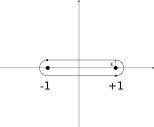
\includegraphics[scale=0.5]{images/racine_carree.png}
    \caption{Contour d'intégration pour la racine carrée.}
    \label{fig:racine_carree}
\end{figure}
En utilisant le résidu à l'infini, on obtient:
\[
\int_{\gamma} = - i 2 \pi \text{Res}_\infty f.
\]
Or:
\[
z\frac{-1}{z^2} \frac{1}{\sqrt{1-z^-2}} = -\frac{1}{\sqrt{z^2-1}}.
\]
En prenant la limite pour $z \to 0$, on en déduit:
\[
\text{Res}_\infty f = -i 2 \pi (i) = 2 \pi.
\]
Finalement, en faisant tendre $\epsilon$ vers $0$, la majoration ML montre que les intégrales sur les arcs de cercle se comportent comme $\sqrt{\epsilon}$ et tendent vers $0$ lorsque $\epsilon$ tend vers $0$. Concernant les intégrales sur les bords horizontaux, on remarque tout d'abord que sur le bord situé dans le demi-plan $\Im(z) < 0$ et avec la détermination choisie pour la racine carrée:
\begin{equation}
    \lim_{y \ to 0^-} \sqrt{1-z^2} \to \sqrt{1-x^2}.
\end{equation}
L'application $z \mapsto 1/\sqrt{1-z^2}$ se prolonge analytiquement dans un voisinage ouvert du segment $]-1,1[.$
En changeant de détermination pour $\sqrt{1-z}$ et pour $\eta>0$ assez petit, en posant $z= 1 + \eta \exp{i \theta},\, \theta \in ]-a,a[, 0 < a < \pi/2$, on peut écrire $\sqrt{1-z} = \sqrt{\eta} e^{i \theta/2}$ qui est bien définie.
L'intégrale le long du contour de la figure \ref{fig:racine_bords} vaut  $0$, l'intégrale sur le bord horizontal inférieur converge donc, pour $\epsilon \to 0^+$, vers:
\[
 \int_{-1}^1 \frac{dx}{\sqrt{1-x^2}}
\]
\begin{figure}
    \centering
    \includegraphics[scale=0.6]{images/contour_racine_bords.png}
    \caption{Bord inférieur de la coupure.}
    \label{fig:racine_bords}
\end{figure}
De même, l'intégral sur le bord supérieur converge vers:
\[
- \int_{-1}^1 \frac{dx}{\sqrt{1-x^2}}.
\] 
En regroupant les termes et en tenant compte de l'orientation, il vient:
\[
\int_{-1}^1 \frac{dx}{\sqrt{1-x^2}} = \pi.
\]
\begin{rem}
La technicité du calcul précédent ne milite pas en faveur de l'intégration dans le plan complexe. Ce n'est plus le cas, toutefois, si l'on s'intéresse à des intégrales de la forme:
\[
\int_0^x \frac{dt}{\sqrt{P(t)}}
\]
où $P$ est une application polynomiale de degré inférieur à $4.$
Toujours en utilisant les techniques présentées plus haut, on peut exprimer ces intégrales à partir des fonctions elliptiques de Jacobi, qui sont aisément calculables numériquement. On les rencontre en particulier lorsque l'on veut déterminer la distance géodésique entre deux points sur un ellipsoïde de révolution.
\end{rem}
\subsection{Intégrales faisant intervenir le logarithme}
Tout comme la racine carrée, le logarithme n'est pas une application holomorphe dans $\C$, il faut introduire une coupure, généralement $\R^-$ ou $\R^+.$ Soit l'application:
\[
f \colon z \mapsto \frac{\ln{z}}{1+z^2}
\]
On choisira de couper le plan complexe par la demi-droite $\R^+$, la détermination étant telle que $\ln(x+iy)_{y \to 0^+, x > 0} \to \ln(x)$ et
$\ln(x+iy)_{y \to 0^-, x > 0} \to \ln(x)+i 2 \pi.$ Sur le contour d'intégration $\gamma$ de la figure \ref{fig:contour_log}, le théorème des résidus donne, pour $R> 1, \epsilon < 1$:
\[
\int_\gamma f(z)dz = i2 \pi \left(
\text{Res}_i f + \text{Res}_{-i} f
\right)
\]
Les deux points singuliers étant des pôles simples, on a directement:
\[
\int_\gamma f(z)dz = i2 \pi \left(
\frac{\ln i}{2 i} + \frac{\ln (-i)}{- 2 i} \right)= (i 2 \pi)\left(- \frac{\pi}{2}\right).
\]
La majoration ML montre que les intégrales sur les deux arcs de cercle tendent vers $0$ pour $R \to +\infty, \epsilon \to O^+$, on en déduit:
\[
\int_{0}^{+\infty}\frac{\ln x}{1+x^2}dx - \int_{0}^{+\infty}\frac{i 2 \pi + \ln x}{1+x^2}dx = - i2 \pi \int_{0}^{+\infty}\frac{dx}{1+x^2}
\]
Soit:
\[
\int_{0}^{+\infty}\frac{dx}{1+x^2} = \frac{\pi}{2}
\]
Par le même procédé, on peut calculer les intégrales:
\[
\int_0^{+\infty} \frac{dx}{1 + x^n}=\frac{\pi}{n\sin{\pi/n}}
\]
En considérant:
\[
g\colon z \mapsto \frac{\ln^2 z}{1+z^n}dz
\]
on obtient également:
\[
\int_0^{+\infty} \frac{\ln x}{1 + x^n} dx = -\frac{\pi^2}{n^2}\frac{\cos{\pi/n}}{\sin^2{\pi/n}}.
\]

Le logarithme est souvent utilisé comme auxiliaire de calcul pour des intégrales sur $\R^+$ ou $\R^-$ ; c'est une technique à connaître.
\begin{figure}
    \centering
    \includegraphics[scale=0.5]{images/contour_log.pdf}
    \caption{Contour d'intégration pour le logarithme complexe.}
    \label{fig:contour_log}
\end{figure}





\section{Exercices complémentaires}

\begin{exer}
Le résidu logarithmique d'une fonction $f(z)$ holomorphe est le résidu de la fonction $f^\prime(z)/f(z)$, dérivée de la fonction $\log f(z)$. 
\begin{MYenumerate}
\item Supposons que $a$ soit un zéro d'ordre $N$ de $f(z)$. Obtenir les premiers termes du développement en série de Laurent de la fonction $f^\prime(z)/f(z)$ et en déduire que $a$ est un pôle du premier ordre de résidu $N$.  
\item Soit $a$ un pôle d'ordre $N$ de $f(z)$. Considérer la fonction $g(z)=-1/f(z)$ et comparer $g^\prime(z)/g(z)$ à $f^\prime(z)/f(z)$. En déduire que $a$ est un pôle du premier ordre de $f^\prime(z)/f(z)$, de résidu $-N$.
\end{MYenumerate}
On a ainsi prouvé qu'aux zéros et aux pôles de $f(z)$, la dérivée logarithmique $f^\prime(z)/f(z)$ possède des pôles du premier ordre. De plus, en un zéro, le résidu logarithmique est égal à l'ordre du zéro, en un pôle à l'ordre du pôle précédé du signe moins.
\end{exer}

\begin{exer}
Soit $f$ une fonction holomorphe dans un domaine borné $\Omega$, sauf en un nombre fini de pôles $b_1,\cdots, b_m$ respectivement d'ordre $p_1, p_2, \cdots, p_m$, continue et ne s'annulant pas sur la frontière de ce domaine. La fonction $f$ a un nombre fini de zéros dans $\Omega$. Désignant par $a_1, a_2, \cdots, a_l$ les zéros respectifs de $f$ d'ordre respectifs $n_1,n_2,\cdots, n_l$.      
\begin{MYenumerate}
\item Appliquer le théorème des résidus à la dérivée logarithmique $f^\prime(z)/f(z)$.
\item En déduire la valeur de $N-P$, où $N$ et $P$ désignent respectivement le nombre de zéros et de pôles de $f$. En outre, chaque zéro et chaque pôle est compté autant de fois que son ordre l'indique.
\end{MYenumerate}
Notons que l'intégrale de la dérivée du logarithme (pour la détermination principale) s'écrit
\[\frac{1}{2 \pi i} \int_\gamma \diff \log f(z)  = \frac{1}{2 \pi i} \int_\gamma \diff \log \lvert f(z)\rvert +\frac{1}{2 \pi i} \int_\gamma \diff \text{arg} f(z).\]
La première intégrale de droite s'annule, tandis que la seconde est la variation totale $\Delta_\gamma \text{arg}f(z)$ de l'argument de $f(z)$, lorsque l'on décrit $\gamma$ divisé par $2 \pi$. Ainsi,
\[N-P=\frac{1}{2 \pi }\Delta_\gamma \text{arg}f(z).\]
\end{exer}

\begin{exer}
Soit $f(z)$ et $g(z)$ deux fonctions holomorphes à l'intérieur d'un contour $C$ donné et continue sur $C$.
\begin{MYenumerate}
\item Montrer que la dérivée logarithmique de $f(z)+g(z)$ est égale à la somme de la dérivée logarithmique de $f(z)$ et de $1+ g(z)/f(z)$.
\item Supposons que $\lvert f(z) \rvert > \lvert g(z) \rvert$ pour tout $z \in C$. En déduire que $\lvert f(z) \rvert > 0$ et $\lvert f(z) + g(z)\rvert >0$ sur $C$.
\item Lorsque $z$ décrit le contour $C$, le point $\omega=1+ g(z)/f(z)$ reste tout le temps dans le cercle $\lvert \omega -1 \rvert <1$. En déduire que le point $\omega$ ne peut faire le tour du point $0$, et donc que 
\[\Delta_C \text{arg}\left\{1 + \frac{g(z)}{f(z)}\right\}=0.\]
\item Conclure que les fonctions $f(z)+g(z)$ et $g(z)$ ont le même nombre de zéros à l'intérieur de $C$ (c'est le théorème de Rouché).
\end{MYenumerate}
\end{exer}


\begin{exer} On souhaite résoudre l'équation $e^z=1+2 z$ dans le disque unité. Une solution évidente est $z=0$, cherchons si il en existe d'autres. Pour cela appliquer le théorème de Rouché avec $f(z)=-2 z$ et $g(z)=e^z-1$.
\end{exer}


\begin{exer}
Le théorème des résidus peut servir à calculer des séries. Par exemple, pour calculer la somme de la série
\[\sum_{n=1}^\infty \frac{x}{n^2 \pi^2-x^2},\]
nous allons étudier l'intégrale 
\[I=\frac{1}{2 \pi i}\int_{C_n} \frac{\cot(w)}{w(w - z)} \diff w,\]
où le contour $C_n$ est le carré de sommets les quatre points $(\pm 1 \pm i)\cdot(n+\frac{1}{2})\cdot\pi$, et $z$ à l'intérieur du contour (donc $n$ assez grand).
\begin{MYenumerate}
\item Déterminer les pôles de la fonction en $w$ intégrée et en calculer les résidus (attention au pôle en zéro).
\item Utiliser le théorème des résidus pour calculer cette intégrale.
\item Majorer le module de $I$ pour $n \gg \lvert z \rvert$, et en déduire que $\lvert I \rvert \to 0$ lorsque $n \to \infty$.
\item En conclure que
\[\sum_{n=1}^\infty \frac{z}{n^2 \pi^2-z^2} = -\frac{1}{2}\cot z + \frac{1}{2 z}.\]
\end{MYenumerate}
\end{exer}

\newpage 
\subsection*{Un peu d'histoire \dots}

\begin{minipage}{0.2\linewidth}
\begin{center}\includegraphics[width=2cm]{images/Laurent.jpg}\end{center}
\end{minipage}
\begin{minipage}{0.80 \linewidth}
\small{\paragraph*{Pierre Alphonse Laurent :} né le 18 juillet 1813 à Paris et mort le 2 septembre 1854 à Paris. Polytechnicien à 19 ans, il commence une carrière militaire et participe aux expéditions de Mascara et de Tlemcen. A son retour, il fut chargé de travaux visant à l'agrandissement du port de Havre. Il exerçait son activité scientifique sur son temps libre. Il contribua en physique à la théorie des ondes et introduisit en analyse complexe le développement en série qui porte son nom.}
\end{minipage}

\vspace*{2cm}


\begin{minipage}{0.2\linewidth}
\begin{center}\includegraphics[width=2cm]{images/Taylor.jpg}\end{center}
\end{minipage}
\begin{minipage}{0.80 \linewidth}
\small{\paragraph*{Brook Taylor :} né à Edmonton (Borough d'Enfield, Londres, Angleterre) le 18 août 1685, et mort à Londres le 29 décembre 1731. Il invente l'intégration par parties et introduit le développement en série des applications différentiables. Il publie en 1715 deux ouvrages fondamentaux : \textit{Methodus incrementorum directa et inversa} dans lequel il aborde le problème des cordes vibrantes ainsi que le calcul des différences finies, et \textit{Linear Perspective}. Cependant, le terme de \textit{série de Taylor} n'apparaîtra qu'en 1786.}
\end{minipage}
\chapter{Transformation de Laplace}
\section{Définition}
Soit $f : \mathbb{R} \to \mathbb{C}$ une application telle que~:
\begin{itemize}
\item $\forall t < 0, \, f(t) = 0$. ($f$ est dite \textit{causale}) 
\item $f$ est intégrable sur tout compact de $\mathbb{R}$.
\item Il existe un réel $x$ tel que l'intégrale~:
\[
\int_{\mathbb{R}^+}e^{-xt} f(t) dt
\]
soit convergente.
\end{itemize}

\begin{fdefn}
Soit $f$ une application vérifiant les conditions précédentes. La
transformée de Laplace de $f$ est l'application $\mathcal{L}(f) : \Omega \subset \mathbb{C} \to
\mathbb{C}$ définie par~:
\[
\mathcal{L}(f)(p) = \int_0^{+\infty}e^{-pt} f(t) dt
\]
$\Omega$ étant l'ensemble des $p$ pour lesquels l'intégrale précédente
est définie.
\end{fdefn}

\begin{fprop}
Si la transformation de Laplace de $f$ est définie pour $p_0$, elle
est également définie pour tout $p$ tel que $\Re(p) > \Re(p_0)$.
\end{fprop} 

La borne inférieure de l'ensemble des $x \in \R$ pour lesquels l'intégrale de
Laplace est convergente pour $\Re(p) = x$ est appelée abscisse de
convergence de la transformation de Laplace. 

On définira de même l'abscisse de convergence absolue, celle de $\vert f \vert$, qui est
supérieure ou égale à l'abscisse de convergence. On remarquera que
chacune de ces bornes peut être $-\infty$.

\begin{fprop}
Soit $p_0$ un complexe tel que la transformée de Laplace $\mathcal{L}(f)(p_0)$ de
$f$ soit définie. Soit $C_{\alpha, p_0}$ l'ensemble des complexes de
la forme $p_0 + r e^{i \theta}$ avec $r \in \mathbb{R}^+$ et $\theta
\in [-\alpha, \alpha]$. L'intégrale de Laplace est uniformément
convergente dans $C_{\alpha, p_0}$ si $\alpha \in ]0, \frac{\pi}{2}[$.
\end{fprop}

\begin{proof}
Soit $\epsilon > 0$ et soit $T > 0$ tel que pour tout $t > T$~:
\[
\lvert \int_T^t e^{-p_0 u}f(u) du \rvert  < \epsilon.
\]
On note $g(t) = \int_T^t e^{-p_0 u}f(u) du$.
Posons $p = p_0 + h$ pour $p \in C_{\alpha, p_0}$ et $h = r e^{i
\theta}$. On a~:
\[
\int_T^t e^{-p u}f(u) du = \int_T^t e^{-hu}g^\prime(u) du.
\]
Une intégration par parties conduit à~:
\[
\int_T^t e^{-hu}g^\prime(u) dt = e^{-ht}g(t) + h \int_T^t e^{-hu}g(u) du.
\]
Pour $t > T$ le premier terme est inférieur en module à $\epsilon$, alors que le
second est borné en module par~:
\[
r \epsilon \int_T^{+\infty} e^{-r u \cos(\alpha)} d u =
\frac{\epsilon}{\cos(\alpha)}.
\]
\end{proof}
La transformation de Laplace est holomorphe dans son domaine de
convergence comme le montre la proposition suivante.

\begin{fprop}
Soit $f$ continue sur $\mathbb{R}^+$ et soit $s$ l'abscisse de
convergence de sa transformée de Laplace $F$. Alors $F$ est
holomorphe dans le demi-plan complexe formé des points de partie
réelle strictement supérieure à $s$.
\end{fprop}

\begin{proof}
Soit $p = x+iy$ avec $x > s$. Soit $p_0 = x_0 + i y$ un point tel
que $s < x_0 < x$. Pour tout $\alpha \in ]0, \frac{\pi}{2}[$, le point
$p$ appartient à $C_{\alpha, p_0}$ et l'intégrale définissant $F$
est uniformément convergente dans $C_{\alpha, p_0}$. De plus,
l'application~:
$
p \mapsto e^{-pt} f(t)
$
est indéfiniment dérivable sur $C_{\alpha, p_0}$ et $t > 0$. On en
déduit alors (dérivation sous le signe somme) que $F(p)$ est
holomorphe dans $C_{\alpha, p_0}$ et que~:
\[
F^{(n)}(p) = (-1)^n \int_0^{+\infty} t^n f(t) e^{-pt} dt.
\] 
\end{proof}
\begin{rem}
La proposition reste vraie si $f$ est seulement continue par morceaux.
\end{rem}
\section{Propriétés}
La transformation de Laplace est de façon évidente linéaire. Son
intérêt principal vient de son comportement vis à vis de la
dérivation.

\begin{fprop}
Soit $f$ continue sur $\mathbb{R}^+$, dérivable. Si elle admet une
transformée de 
Laplace ainsi que sa dérivée, les deux transformées
sont liées par la relation~:
\[
\mathcal{L}(f^\prime)(p) = p \mathcal{L}(f)(p) - f(0^+)
\] 
avec $f(0^+) = \lim_{ t \to 0, \; t > 0} f(t)$
\end{fprop}

\begin{proof}
On a~:
\[
\mathcal{L}(f^\prime)(p) = \lim_{t\to + \infty} \int_0^Tf^\prime(t) e^{-pt} dt.
\]
Une intégration par parties montre que l'intégrale de droite vaut~:
\[
\left [
e^{-pt}f(t)
\right ]_0^T
+ p \int_0^T f(t) e^{-pt} dt.
\]
Qui montre la proposition par passage à la limite.
\end{proof}
Cette proposition s'étend par récurrence pour les dérivées d'ordre
quelconque~:
\[
\mathcal{L}(f^{(n)})(p) = p^n \mathcal{L}(f)(p) - p^{n-1} f(0)
- p^{n-2} f^\prime(0) - \dots f^{(n-1)}(0^+)).
\]
Il est possible de déterminer également la transformée de Laplace de
la primitive d'une application.

\begin{fprop}
Si $f$ admet une transformée de Laplace $F$ et si $\lim_{t \to 0^+}
\frac{f(t)}{t}$ existe, alors~:
\[
\mathcal{L} \left( \frac{f(t)}{t} \right) (p) = \int_p^{+\infty} F(u) du.
\]
\end{fprop} 

\begin{proof}
\[
\int_p^Z F(u) du = \int_p^Z \int_0^{+\infty} e^{-ut}
f(t) dt du
\]
comme l'intégrale de Laplace est uniformément convergente dans un
secteur angulaire, on peut intervertir l'ordre de intégrations et
l'intégrale devient~:
\[
\int_0^{+\infty} e^{-pt} \frac{f(t)}{t} dt - \int_0^{+\infty} e^{-Zt} \frac{f(t)}{t} dt
\] 
La conclusion s'obtient en faisant tendre $Z$ vers l'infini en module.
\end{proof}

\begin{fprop}
Soit $f$ de transformée de Laplace $F$ et soit $s$ l'abscisse de
convergence de cette transformée. Alors l'application~:
\[
\int_0^t f(u) du
\]
admet pour transformée de Laplace $\frac{F(p)}{p}$ et son abscisse de
convergence est strictement supérieure à $\sup(0, s)$.
\end{fprop}

Cette proposition se montre de façon similaire à la précédente.
\begin{fprop}
Soit $f$ admettant une transformée de Laplace $F$ d'abscisse de
convergence $s$. Soit $a \in \mathbb{C}$. Alors l'application
$e^{at}f(t)$ admet pour transformée de Laplace $F(p-a)$, son abscisse
de convergence étant $s + \Re(a)$.
\end{fprop}
\begin{fprop}
Soit $f$ admettant $F$ pour transformée de Laplace. Soit $a \in
\mathbb{R}$. Alors
l'application $g$ telle que $g(t) = 0$ si $t < a$ et $g(t) = f(t-a)$
sinon admet pour transforméee de Laplace $e^{-ap}F(p)$.
\end{fprop}
Ces deux propositions se montrent de manière immédiate.
On peut calculer facilement à partir de ceci la transformée de Laplace
d'une application périodique. Soit $f_1$ une application à support
dans un intervalle réel $[0,T]$ et soit $f$ l'application définie par
périodisation de $f_1$ de période $T$. Si $f$ admet une transformée de
Laplace et si $F_1$ est la transformée de Laplace de $f_1$, alors~:
\[
\mathcal{L}(f)(p) = \frac{F_1(p)}{1-e^{-pT}}.
\]
Ce résultat s'obtient en écrivant $f$ sous la forme d'une somme de
termes de la forme $f_1(t-k T)$ avec $k \in \mathbb{N}$ et en faisant
apparaître une série géométrique.
On a enfin une proposition relative aux changements d'échelle.
\begin{fprop}
Si $f$ admet pour transformée de Laplace $F$ alors, pour $\lambda \in
\mathbb{R^*}$, l'application $f\left( t/\lambda \right)$ admet pour transformée de
Laplace $\lambda F(\lambda p).$
\end{fprop}
\section{Inversion}

\begin{fprop}(Théorème de la valeur finale)
Soit $f$ continue de transformée de Laplace $F$. Si l'abscisse de convergence
$s$ est négative et si $\lim_{t \to +\infty}f(t)$ existe, alors~:
\[
\lim_{p \to 0^+} p F(p) = \lim_{t \to +\infty} f(t).
\]
\end{fprop}

\begin{proof}
Soit $l = \lim_{t \to +\infty} f(t)$. 
\begin{align*}
pF(p) - l & = p \int_0^{+\infty} e^{-pt}f(t) dt - l \\
&= p \int_0^T  e^{-pt}f(t) dt + p  \int_T^{+\infty}e^{-pt}(f(t) -l) dt
\\ &+ l \left (
p \int_T^{+\infty} e^{-pt}dt -1
\right )
\end{align*}
Le premier terme est majoré en module par~:
\[
|p| T M_T
\]
avec $M_T$ borne $\sup$ de $|f|$ sur $[0,T]$.
Le second terme se majore uniformément par définition de la limite de
$f$ en $+\infty$ et la convergence uniforme de l'intégrale. Enfin, le
troisième terme tend vers 0 pour $|p|\to 0^+$, ce qui montre la proposition.
\end{proof}

\begin{fprop}(Théorème de la valeur initiale)
Soit $f$ dérivable, de transforméee de Laplace $F$ et telle que sa
dérivée soit également transformable. Alors~:
\[
\lim_{|p|\to +\infty} p F(p) = f(0^+)
\]
\end{fprop}

\begin{proof}
On a~:
\[
\lim_{|p| \to +\infty} \mathcal{L}(f^\prime)(p) = 0
\]
et $\mathcal{L}(f^\prime)(p) = p F(p) - f(0^+)$.
\end{proof}

\begin{fprop}
Soit $f$ définie par une série entiére convergente $\sum_{n \in
\mathbb{N}} a_n z^n$ de rayon de convergence infini. Alors elle
est transformable et sa transformée s'obtient en transformant terme à terme.
\end{fprop}

\begin{fdefn}
Soit $[a,b]$ un intervalle de $\mathbb{R}$. Soit $f : [a,b] \to \mathbb{R} (\mbox{ resp. } \mathbb{C})$. On dira
que $f$ est à variation bornée si~:
\[
\sup \{ \sum_{i=0\dots N-1} |f(t_{i+1}) - f(t_i)|, \, a = t_0 < t_1, \dots < t_N = b, \, N \in \mathbb{N} \} < + \infty
\]
\end{fdefn}
La définition précédente s'étend immédiatement au cas des intervalles semi-infinis ou infinis.
La proposition suivante est très classique~:
\begin{fprop}(Lemme de Dirichlet)
Soit $f$ à variation bornée sur un intervalle $[0,a]$. On a~:
\[
\lim_{b \to +\infty} \int_{[0,a]} f(x) \frac{\sin bx}{x} d \lambda(x) =
f(0^+) \lim_{T \to +\infty} \int_{[0,T]} \frac{\sin x}{x} d \lambda(x).
\]
\end{fprop}

\begin{fthm}
Soit $F$ la transformée de Laplace d'une application à variation bornée $f$, l'abscisse
de convergence étant $s$. En tout point de continuité $t$ de $f$, on a~:
\[
f(t) = \frac{1}{i 2 \pi} \lim_{b \to + \infty} \int_{a-ib}^{a+ib}
e^{pt} F(p) dp
\]
avec $a > s$.
\end{fthm}

\begin{proof}
Formons~:
\[
f_b(t) = \frac{1}{i 2 \pi}  \int_{a-ib}^{a+ib} e^{pt} \int_0^{\infty}
e^{-pu} f(u) du dp.
\]
La convergence de l'intégrale étant uniforme, on peut écrire, après
interversion des intégrales~:
\[
f_b(t) = \frac{1}{\pi} e^{at} \int_{-t}^{+\infty} f(u+t)e^{-a(u+t)}
\frac{\sin (b u)}{u} du.
\]
Comme par ailleurs $f(t) = 0$ pour $t < 0$, on a~:
\[
f_b(t) = \frac{1}{\pi} e^{at} \int_{-\infty}^{+\infty} f(u+t)e^{-a(u+t)}
\frac{\sin (b u)}{u} du.
\]
Soit encore~:
\[
f_b(t) = \frac{1}{\pi} e^{at} \int_{0}^{+\infty} \left (
f(u+t)e^{-a(u+t)} + f(t-u)e^{-a(t-u)}
\right )
\frac{\sin (b u)}{u} du.
\]
En utilisant~:
\[
\int_0^{+\infty} \frac{\sin (b u)}{u} du = \frac{\pi}{2}
\]
on obtient~:
\[
f_b(t) = f(t)  + \frac{1}{\pi} e^{at} \int_{0}^{+\infty} \left (
f(u+t)e^{-a(u+t)} + f(t-u)e^{-a(t-u)} - 2 f(t)e^{-at}
\right )
\frac{\sin (b u)}{u} du.
\]
Le résultat s'obtient alors en faisant tendre $b$ vers $+\infty$ et en utilisant le lemme de Dirichlet.
\end{proof} 
Il existe une forme réciproque de ce théorème~:

\begin{fthm}(Formule d'inversion de Mellin-Fourier)
Soit une application $F$ analytique dans un demi-plan $\Re(p) > s_0$,
tendant vers 0 pour $|p| \to +\infty$ dans tout demi-plan $\Re(p) > s
> s_0$. Si l'intégrale~:
\[
\int_{s-i \infty}^{s+i \infty} F(p) dp
\]
converge absolument pour $s > s_0$, alors $F$ est la transformée de
Laplace de l'application $f$ définie par~:
\[
f(t) = \frac{1}{i 2 \pi} \int_{s-i \infty}^{s+i \infty} F(p) dp.
\]
On dira que $f$ est l'original de $F.$
\end{fthm}

Le contour de la figure \ref{fig:contour_laplace} (contour de Bromwich-Wagner) est fréquemment employé pour calculer l'original d'une transformée de Laplace par la formule de Mellin-Fourier.
\begin{figure}
    \centering
    \includegraphics[scale=0.8]{images/contour_laplace.png}
    \caption{Contour de Bromwich-Wagner pour la transformée de Laplace inverse.}
    \label{fig:contour_laplace}
\end{figure}
En pratique, on inversera le plus souvent une transformée de Laplace en utilisant des tables, ou un logiciel de calcul formel comme \texttt{Mathematica}.

\begin{exercice}
On veut déterminer l'original de l'application~:
\[
F : p \to \frac{1}{1+p^3}
\]
\begin{itemize}
\item Calculer, en précisant l'abscisse de convergence, la transformée de Laplace de l'application:
\[
f \colon t \mapsto \begin{cases}
    0 & t< 0 \\
    e^{-at} & t \geq 0, a \in \C
\end{cases}
\]
\item Décomposer $F$ en éléments simples et en déduire son original $f.$
\item Retrouver ce résultat par la formule d'inversion de Mellin-Fourier.
\end{itemize}
\end{exercice}

\newpage 
\subsection*{Un peu d'histoire \dots}

\begin{minipage}{0.2\linewidth}
\begin{center}\includegraphics[width=2.9cm]{images/Laplace.jpeg}\end{center}
\end{minipage}
\begin{minipage}{0.8 \linewidth}
\small{\paragraph*{Pierre-Simon, marquis de Laplace :} né le 23 mars 1749 à Beaumont-en-Auge (Calvados) et mort le 5 mars 1827 à Paris, est un mathématicien, astronome, physicien et homme politique français. Il utilisa une notion proche de la transformation portant son nom en 1774 dans le cadre de ses travaux sur la théorie des probabilités. Pour Laplace, la nature est l'essence de la découverte scientifique et les mathématiques ne sont qu'un instrument pour la décrire. Laplace est avant tout un théoricien de l'astronomie, mais sa passion pour cette discipline est le prétexte à de nombreuses études mathématiques, en particulier dans le domaine des équations différentielles et en théorie des probabilités. 

Peu intéressé par les idées révolutionnaires, il reste politiquement neutre. Napoléon entretient de bons rapports avec lui et le nomme Ministre de l'Intérieur en 1799, poste qu'il n'occupera qu'un mois. Plus tard, Napoléon lui reprochant de ne pas citer Dieu dans son \textit{Traité de Mécanique Céleste} (1812), Laplace lui répond : "Je n'ai pas besoin de cette hypothèse".  
}
\end{minipage}

\vfill
\chapter{Surfaces de Riemann}
\section{Un exemple: la racine carrée}
Soit à calculer l'intégrale suivante:
\[
I = \int_{\mathcal{C}(0,1)} \frac{dz}{2 \sqrt{z}}
\]
où $\mathcal{C}(0,1)$ est le cercle unité parcouru une seule fois en sens trigonométrique. La formule donnant l'intégrale d'une application continue le long d'un chemin de classe $C^1$ donne:
\[
I = \frac{1}{2} \int_0^{2\pi} i e^{it}e^{-it/2} dt = \frac{i}{2} \int_0^{2\pi} e^{it/2} dt= -2
\]
Si l'on parcourt maintenant deux fois le même contour, l'application de la même formule conduit à un résultat pour le moins surprenant:
\[
\frac{i}{2} \int_{0}^{4 \pi} e^{it/2} dt= 0 \neq 2 I 
\]
Que s'est-il donc passé ? Une clé de compréhension de ce phénomène est donnée par la proposition suivante:
\begin{prop}
Il n'existe pas d'application continue $f \colon \C \to \C$ telle que $f^2(z) = z$.
\end{prop}
\begin{proof}
Soit $f$ vérifiant pour tout $z\in \C$: $f^2(z)=z$. En écrivant $z$ sous forme polaire, il vient:
\[
f^2\left(r e^{it}\right) = r e^{it}
\]
soit encore:
\[
f\left(r e^{it}\right) = \sqrt{r} e^{it/2} \text{ (détermination positive)}
\]
ou:
\[
f\left(r e^{it}\right) = - \sqrt{r} e^{it/2} \text{ (détermination négative)}
\]
Soit $\gamma \colon t \in [0,2\pi] \mapsto e^{it}$ un paramétrage du cercle unité. On a $f\circ \gamma(0^+)= 1 (\text{resp.} -1) \neq f\circ \gamma(2 \pi^-)= f \circ \gamma(2\pi^-)=-1(\text{resp.} 1)$, prouvant ainsi que $f$ ne peut être continue.
\end{proof}
Un problème similaire avait été rencontré dans le cas du logarithme complexe et se résout classiquement par l'introduction d'une coupure. Dans le cas de la racine carrée, on choisit généralement de supprimer l'axe réel négatif pour conserver la définition usuelle, mais il n'existe que deux déterminations (alors qu'il en existe une infinité pour le log) :
\[
\begin{cases}
&\sqrt{r e^{it}}_+ = \sqrt{r} e^{it/2} \\
&\sqrt{r e^{it}}_- = -\sqrt{r} e^{it/2}
\end{cases}
\]
Cela interdit néanmoins le contour d'intégration $\mathcal{C}(0,1)$, que l'on peut cependant voir comme une intégrale généralisée, avec le paramétrage $\gamma \colon t \in ]-\pi,\pi[ \to e^{it}$:
\[
\frac{i}{2} \int_{-\pi^+}^{\pi^-} e^{it/2} dt = 2i
\]
Le résultat obtenu est différent de celui obtenu pour $I$, ce qui n'est guère satisfaisant. Toute la difficulté réside dans le fait que l'application "racine carrée" n'est pas correctement définie sur $\C$, tout comme d'ailleurs sur $\R$. Si l'on cherche en effet à résoudre l'équation $w^2 = z$ avec $(z,w)\in \C$, on obtient non pas le graphe d'une fonction, mais une surface de $\C^2$, formée des couples $(z=r e^{it},w=\pm \sqrt{r} e^{it/2})$. L'image \ref{fig:sqrt_} correspond à la partie réelle de la coordonnée $w$ de cette surface.
%\footnote{Crédit:  Wlongqi - Own work, CC BY-SA 3.0, \url{https://commons.wikimedia.org/w/index.php?curid=5964270}}

%\begin{figure}[h]
%	\centering
%	\includegraphics[scale=0.3]{Riemann_sqrt.png}
%	\caption{Partie réelle de la surface $w^2=z$}
%\end{figure}

\begin{figure}[hbt]
\begin{center}\includegraphics[scale=0.46]{images/Surf_Riema_sqrt_Re_positive.PNG}
\end{center}
\caption{Partie réelle de la surface $w^2=z$, détermination positive}\label{fig:sqrt_positive}
\end{figure}

\begin{figure}[hbt]
\begin{center}\includegraphics[scale=0.46]{images/Surf_Riema_sqrt_Re.PNG}
\end{center}
\caption{Partie réelle de la surface $w^2=z$}\label{fig:sqrt_}
\end{figure}

L'idée (due à B. Riemann) qui va maintenant être formalisée, consiste à remplacer l'intégration dans $\C$ par une intégration dans $\C^2$ en se restreignant à la surface de Riemann.
\section{Surfaces de Riemann abstraites}
Une surface de Riemann définie de façon générale est une abstraction de la notion de surface concrète dans $\C^2$. Dans la plupart des cas, il sera cependant possible d'en obtenir une image locale sous la forme d'un graphe de fonction. Le point de départ de la théorie est la proposition suivante.
\begin{prop}
	\label{prop:chg_var}
	Soit $\Omega$ un domaine de $\C$ et soit $\phi \colon \Omega ( \subseteq \C) \to \phi(\Omega) (\subseteq \C)$ une bijection holomorphe ainsi que son application réciproque. Pour tout chemin $\gamma \colon [a,b] \to \Omega$ et toute application continue $f \colon \phi(\Omega) \to \C$, on a:
	\[
	\int_{\phi \circ \gamma} f(z)dz = \int_\gamma f \circ \phi(z) \phi^\prime(z)dz
	\]
\end{prop}
\begin{proof}
	Il s'agit d'une application directe du théorème des fonctions composées. On a:
	\[
	\int_{\phi \circ \gamma} f(z)dz = \int_a^b f\left(\phi \circ \gamma(t)\right)\phi^\prime(\gamma(t)) \gamma^\prime(t) dt = \int_\gamma f \circ \phi(z) \phi^\prime(z)dz
	\]
\end{proof}
A partir de ce résultat, on remarque qu'une intégrale de chemin peut se définir soit sur le domaine, soit sur l'image du domaine par un difféomorphisme de $\C$.
\begin{fdefn}
	Une surface de Riemann est un espace topologique connexe $X$ pour lequel il existe une famille d'ouverts $(U_i)_{i \in I}$ recouvrant $X$ et des homéomorphismes $(\phi_i)_{i \in I} \colon U_i \to V_i$ avec $(V_i)_{i \in I}$ ouverts de $\C$ telles que les applications:
	\begin{align*}
	    \psi_i^j \colon \phi_i (U_j\cap U_i) & \longrightarrow  \phi_j (U_i\cap U_j), \,  \forall(i,j) \in I^2, \\
	    z  & \longmapsto \phi_j\circ \phi_i^{-1}(z)
	\end{align*}
	soient holomorphes ainsi que leurs applications réciproques (on dit encore qu'elle sont biholomorphes).
\end{fdefn}
\begin{defn}
Les applications  $\phi_i$ définies ci-dessus sont les \textbf{cartes locales} de $X$, les applications $\psi_i^j$ définies ci-dessus sont les applications de changement de carte.
\end{defn}
\begin{exem}
Soit $\Omega \subset \C$ un domaine. C'est une surface de Riemann avec l'unique carte locale $\phi \colon z \in \Omega \mapsto z$ ($\phi$ est donc l'application identité).
\end{exem}
\begin{exem}
La sphère de Riemann $\overline{\C}$ offre un exemple non trivial de surface de Riemann. Deux cartes locales sont nécessaires:
\[
    \phi_1 \colon z \in \overline{\C} \setminus \{\omega\} \mapsto z \in \C
\]
et
\[
\phi_2 \colon z \in \overline{\C} \setminus \{0\} \mapsto 1/z
\]
avec la convention $1/\omega=0$ assurant la continuité. Les applications de changement de carte sont:
\[
\psi_1^2 =\psi_2^1 \colon z \in \overline{\C} \setminus \{\omega,0\} \mapsto 1/z
\]
qui sont holomorphes sur leur domaine de définition.
\end{exem}
\begin{defn}
	Soit $X$ une surface de Riemann et $\Omega$ un ouvert de $X$. On dira que $f \colon \Omega \to \C$ est continue (resp. holomorphe) si pour tout $i \in I$, $f \circ \phi_i^{-1}$ est continue (resp. holomorphe) sur $\phi_i(U_i \cap \Omega)$.
\end{defn}
On notera que l'on peut définir une application continue (resp. holomorphe) sur $X$ en considérant une famille $f_i \colon V_i \to \C, i \in I$ vérifiant pour tout couple $(i,j)\in I^2$:
\[
\forall z \in \phi_i(U_i \cap \Omega), f_i(z) = f_j \circ \psi_i^j(z)
\]
Il suffit alors de poser $f(z)=f_i \circ \phi_i(z), z \in \Omega \cap U_i$.
\begin{defn}
Soient $X,Y$ deux surfaces de Riemann et $f \colon X \to Y$. On dira que $f$ est continue (resp. holomorphe) si pour tout couple de cartes locales $\phi_i \colon U_i \to \phi(U_i), \phi_j \colon W_j \to \phi(W_j)$, l'application $\phi_j \circ f \circ \phi_i^{-1}$ est continue (resp. holomorphe).
\end{defn}
\begin{rem}
On peut étendre immédiatement cette définition au cas où l'application $f$ est définie seulement sur un ouvert de $X$.
\end{rem}
\begin{prop}
Les applications holomorphes $f \colon \Omega \to \overline{\C}$, avec $\Omega$ ouvert de $\C$ sont les applications holomorphes de $\Omega \to \C$ ou les applications n'admettant que des pôles comme points singuliers. 
\end{prop}
\begin{proof}
    Il est clair que si $f$ est holomorphe de $\C$ dans $\C$, alors elle est holomorphe dans $\overline{\C}$. Sinon, il existe des points où $f$ est non bornée. Au voisinage de l'un ces points, noté $z_0$, l'application lue dans la carte $\phi_2$ est $1/f$ et par continuité on aura $1/f(z_0) = 0$. Comme $1/f$ est holomorphe et n'est pas identiquement nulle, elle s'exprime sous la forme $1/f(z_0) = (z-z_0)^p g(z)$ avec $g$ ne s'annulant pas dans un voisinage de $z_0$. On en déduit immédiatement que $z_0$ est un pôle d'ordre au plus $p$ de $f$. 
\end{proof}
\begin{rem}
Les applications holomorphes de $\C$  dans $\overline{\C}$ sont appelées applications méromorphes.
\end{rem}
\begin{prop}
\label{prop:surface_racine}
L'ensemble $\mathcal{S}$ des couples $(z,w) \in \C^2$ tels que $w^2=z$ est une surface de Riemann.
\end{prop}
\begin{proof}
La topologie induite sur $\mathcal{S}$ est celle pour laquelle une partie $U$ de $\mathcal{S}$ est ouverte si et seulement si elle est l'intersection d'un ouvert de $\C^2$ avec $\mathcal{S}$. On va considérer trois ouverts et les cartes locales associées:
\[
\left \{
%\begin{cases}
\begin{array}{r c l}
\phi_1 \colon  U_1 = \{ (z,w)\in \mathcal{S}\, | \, \Re \text{e}(w) > 0 \}  &\to&  \C \setminus \R^-\\
 (z, w)  &\mapsto&  z \\
\phi_2 \colon  U_2 = \{ (z,w)\in \mathcal{S}\, | \, \Re \text{e}(w) < 0 \} &\to& \C \setminus \R^-\\
 (z, w)  &\mapsto&  z \\
\phi_3 \colon U_3 = \{ (z,w)\in \mathcal{S}\, | \, \Re \text{e}(w) \in ]-2,2[ \} &\to& ]-2,2[ + i \R \\
 (z, w)  &\mapsto&  w \\ 
\end{array}
\right .
%\end{cases}
\]
Les deux applications de changement de carte à considérer sont $\psi_3^1 = \phi_1 \circ \phi_3^{-1}$ et $\psi_3^2 = \phi_2 \circ \phi_3^{-1}$ vérifiant:
\[
\begin{cases}
\begin{array}{rccl}
\psi_3^1 \colon & ]0,2[ + i \R & \longrightarrow  \C \\
& w & \longmapsto  w^2 \\
\psi_3^2 \colon & ]-2,0[ + i \R & \longrightarrow  \C \\
& w & \longmapsto  w^2    
\end{array}

\end{cases}
\]
Leurs domaines respectifs excluant l'axe imaginaire, il s'agit bien d'applications biholomorphes. 
\end{proof}
\begin{defn}
\label{def:forme_degre_un}
Soit $X$ une surface de Riemann dont la famille des cartes locales est $(U_i,\phi_i)_{i \in I}$. Une forme différentielle $f$ de degré un sur un ouvert $\Omega \subset X$ est la donnée d'une famille d'applications continues $f_i \colon \phi_i(U_i \cap \Omega) \to \C, i \in I$ vérifiant la condition:
\[
\forall (i,j)\in I^2, \forall z \in \phi_i\left(U_i\cap U_j \cap \Omega\right), f_j\left(\psi_i^j(z)\right)\left(\partial_z \psi_i^j(z)\right)=f_i(z)
\]
\end{defn}
\begin{rem}
On notera dans la suite $f_i dz$ la forme différentielle dans l'ouvert $\phi_i(U_i\cap \Omega)$. Cette notation est cohérente avec la notion d'intégrale le long d'un chemin qui sera l'objet de la définition suivante. 
\end{rem}
On dira qu'un chemin $\gamma \colon [a,b] \to X$ est de classe $C^1$ si pour toute carte locale $(U_i,\phi_i)$ telle que $U_i \cap \gamma([a,b]) \neq \emptyset$, $\phi_i \circ \gamma$ est de classe $C^1$.
\begin{defn}
\label{def:integrale_chemin_riemann}
Soit $X$ une surface de Riemann dont la famille des cartes locales est $(U_i,\phi_i)_{i \in I}$. Soit $f = \{f_i\}_{i \in I}$ une forme différentielle de degré $1$ sur un ouvert $\Omega \subset X$ et soit pour $j \in I$ fixé, $\gamma \colon [a,b] \to U_j \cap \Omega$ un chemin. On pose:
\[
\int_{\gamma} f_i(z) dz = \int_a^b f_i\left(\phi_i\circ \gamma(t)\right)\frac{d}{dt}\left(\phi_i\circ \gamma\right)(t) dt
\]
\end{defn}
Cette définition est compatible avec le système de cartes locales comme le montre la proposition suivante.
\begin{prop}
\label{prop:invariance_carte}
Soit $(i,j) \in I^2$ fixé. Soit $f_i, i \in I$ une forme différentielle de degré $1$ sur un ouvert $\Omega \subset X$ et $\gamma \colon [a,b] \to U_i \cap U_j \cap \Omega$ un chemin de classe $C^1$. Alors
\[
\int_\gamma f_i(z) dz = \int_\gamma f_j(z) dz
\]
\end{prop}
\begin{proof}
Il s'agit d'une application directe de la formule du changement de variable dans $\R$:
\[
\begin{split}
 \int_{\gamma} f_j(z) dz & = \int_a^b f_j\left(\phi_j\circ \gamma(t)\right)\frac{d}{dt}\left(\phi_j\circ \gamma\right)(t) dt  \\
& = \int_a^b f_i\left(\psi_i^j\circ \phi_j\circ \gamma(t)\right)\frac{d}{dt}\left(\psi_i^j\circ \phi_i\circ \gamma\right)(t) dt  \\
& = \int_a^b f_j\left(\psi_i^j \circ \phi_j\circ \gamma(t)\right)(\partial_z\psi_i^j(z))\frac{d}{dt} \left(\phi_i\circ \gamma\right)(t) dt  =\int_{\gamma} f_i(z) dz
\end{split}
\]
\end{proof}
La proposition \ref{prop:invariance_carte} montre qu'il est possible de définir l'intégrale d'une forme différentielle de degré 1 sur un ouvert de $X$ en sommant les contributions dans chacune des cartes locales. 
\begin{defn}
On dira qu'une forme différentielle de degré $1$ sur un ouvert $\Omega$ admet une primitive locale si pour toute carte  $(U_i,\phi_i)$ vérifiant $U_i\cap \Omega \neq \emptyset$, l'application $f_i$ admet une primitive locale.
\end{defn}
L'existence d'une primitive locale permet de construire une intégrale le long d'un chemin quelconque de $X$ en suivant le procédé de la proposition \ref{prop:primitive_chemin}. On en déduit donc que toute fonction holomorphe (resp. méromorphe) admet une intégrale le long de tout chemin (resp. ne passant pas par les points singuliers). Par ailleurs, le théorème des résidus continuera à s'appliquer dans chaque carte locale, donc globalement en raison des relations de compatibilité. Ceci va permettre de lever les apparentes contradictions rencontrées lors de l'introduction. 

Revenons à l'exemple introductif dans lequel nous cherchions à intégrer $z \mapsto \frac{1}{\sqrt{z}}$. En se plaçant sur la surface de Riemann associée à la racine carrée visualisée sur la figure \ref{fig:sqrt_}, et en choisissant dans la carte $1$ de la proposition \ref{prop:surface_racine}:
\[
f_1 \colon z = r e^{i \theta} (\theta \in ]-\pi, \pi [)  \mapsto \frac{1}{\sqrt{r}}e^{-i \theta / 2} dz
\]
il vient, en appliquant les règles des formes différentielles:
\[
f_3 \colon w \mapsto 2 \frac{w}{w} dw = 2 dw
\]
et, en remarquant que $\psi_2^3(z)=\sqrt{z}_-$;
\[
f_2 \colon z = r e^{i \theta} (\theta \in ]-\pi, \pi [)  \mapsto \frac{-1}{\sqrt{r}}e^{-i \theta / 2} dz
\]
On remarque tout d'abord que le lacet $\gamma \colon t \in [-\pi,\pi] \mapsto e^{it}$ se relève par les cartes $\phi_1^{-1},\phi_3^{-1}$ en un chemin dans la surface de Riemann. En effet, il s'identifie dans $U_1\cap U_3$ à l'application continue:
\[
\gamma \colon t \in [-\pi,\pi] \mapsto
\begin{cases}
&\left(e^{it},e^{i t /2}\right), \, t \in ]-\pi,\pi[ \\
& \left(-1, -i \right), \, t = -\pi \\
& \left(1, i \right),  \, t = \pi \\
\end{cases}
\]
En remarquant que l'on peut exclure les points extrêmes du chemin sans changer la valeur de l'intégrale, on peut se limiter à la partie appartement à $U_1$. Par la formule d'intégration sur $\phi_1(U_1)$ on obtient:
\[
\int_\gamma f_1(z)dz = \int_{-\pi}^{\pi} e^{-it/2} i e^{it} dt = 4i
\]

On peut également choisir de relever $\gamma$ dans $U_2 \cap U_3$ en utilisant $\phi_2^{-1}$, ce qui donne:
\[
\gamma \colon t \in [-\pi,\pi] \mapsto
\begin{cases}
&\left(e^{it},-e^{i t /2}\right), \, t \in ]-\pi,\pi[ \\
& (-1,i) , \, t = -\pi \\
& (-1,-i),  \, t = \pi \\
\end{cases}
\]
On remarque que le chemin obtenu est différent du précédent et est orienté en sens inverse. 
Si l'on s'intéresse maintenant à ce qui se passe dans la carte $f_2$, il vient:
\[
\int_\gamma f_2(z)dz = \int_{-\pi}^{\pi} -e^{-it/2} i e^{it} dt = -4i
\]
Le résultat est cohérent avec l'orientation du chemin et le fait que la concaténation des relèvements dans $U_1\cap U_3$ et $U_2 \cap U_3$ donne un lacet dans la surface de Riemann. 
En reprenant l'exemple introductif, on peut chercher à relever le lacet $\gamma \colon t \in [0, 2\pi] \mapsto e^{it}$. On peut utiliser soit le couple de cartes $(U_1,\phi_1),(U_2,\phi_2)$ en s'assurant de la continuité ou la carte $(U_3,\phi_3$. Dans le premier cas, l'intégrale le long de $\gamma$ se calcule en deux parties:
\[
\int_0^\pi e^{-it/2}i e^{it}dt + \int_{-\pi,0} -e^{-it/2}e^{it} dt
\]
On remarque que $e^{i\pi/2}=-e^{-i\pi/2}$, la continuité est donc garantie. La première intégrale donne $2(i-1)$, la seconde $2(1+i)$, conduisant à un résultat final de $-4$, en adéquation avec ce qui avait été obtenu précédemment. 
Dans la carte $(U_3,\phi_3)$, le relèvement est le chemin:
\[
(e^{i2t},e^{it}), \, t \in [0, \pi]
\]
L'application des règles d'intégration donne:
\[
\int_0^\pi 2 i e^{it} dt = -4
\]
On retrouve comme attendu le même résultat qu'avec le calcul dans les cartes $(U_1,\phi_1),(U_2,\phi_2)$.
Finalement, le lacet $\gamma ([0, 4\pi])$ se relève directement dans la carte $(U_3,\phi_3)$ en un lacet:
\[
(e^{i2t},e^{it}), \, t \in [0, 2\pi]
\]
Il vient donc:
\[
\int_0^{2\pi} 2 i e^{it} dt = 0
\]
L'utilisation de l'intégrale sur une surface de Riemann adéquate lève toutes les ambiguïtés remarquées dans l'introduction. 
\begin{defn}
Une forme différentielle de degré 1 sera dite holomorphe si elle est holomorphe dans toutes les cartes. Une forme différentielle $f$ sera dite méromorphe dans un ouvert $\Omega$ d'une surface de Riemann $X$ si il existe $\{z_1,\dots,z_n\} \subset \Omega$ telle que $f$ soit holomorphe dans $\Omega \setminus \{z_1,\dots,z_n\}$ et que dans chaque carte les points $z_i,i=1\dots n$ soient des pôles. Il est équivalent de dire que la forme différentielle $f$ est holomorphe lorsqu'elle prend ses valeurs dans la sphère de Riemann. 
\end{defn}
\begin{theorem}{(Théorème des résidus)}
\label{thm:residus_riemann}
Soit $X$ une surface de Riemann compacte et $f$ une forme différentielle méromorphe de degré $1$ dont les points singuliers sont $\{z_1,\dots z_n\}$. On a:
\[
\sum_{i=1\dots n} \text{res}_{z_i} f  = 0
\]
le résidu en $z_i$ étant calculé dans l'une quelconque des cartes dont le domaine contient $z_i$.
\end{theorem}
\begin{proof}
Les intégrales relatives aux formes différentielles de degré 1 ne dépendant pas de la carte locale choisie pour la représenter, on se placera dans la suite en coordonnées locales. Soit $z_i, i=1\dots n$. Il existe un disque fermé centré sur $z_i$ de rayon non nul, noté $\overline{D}_i$, entièrement contenu dans l'image d'une carte locale. On peut lui appliquer le théorème des résidus de $\C$ pour obtenir:
\[
\text{res}_{z_i}f = \frac{1}{i 2\pi} \int_{\partial D_i} f(z) dz
\]
Par ailleurs, $X$ étant compacte, $X \setminus \cup_{i=1,\dots,n} \stackrel{\circ}{D_i}$ est aussi compact, donc recouvert par un nombre fini de cartes locales. On peut ainsi trouver un lacet simple $\gamma$ tel que représenté figure \ref{fig:lacet_riemann_compact} sur lequel l'intégrale est nulle. La conclusion s'ensuit par identification des intégrales, en prenant la limite du lacet $\gamma$ lorsque les bords supérieurs et inférieurs des segments tendent vers une valeur commune.
\begin{figure}[ht]
    \centering
    \includegraphics[scale=0.4]{images/lacet_compact.pdf}
    \caption{Lacet dans $X \setminus \cup_{i=1,\dots,n} \stackrel{\circ}{D_i}$}
    \label{fig:lacet_riemann_compact}
\end{figure}
\end{proof}

Un cas particulièrement important en pratique est celui de la sphère de Riemann, dont les application de changement de carte sont toutes deux $z \mapsto 1/z$. Si $f$ est une application méromorphe sur $\C$, elle définit une forme différentielle méromorphe de degré $1$ sur la carte identité et son expression dans la carte $z \mapsto 1/z$ est:
\[
g \colon z \neq 0 \mapsto \frac{-1}{z^2}f\left(\frac{1}{z}\right)
\]
En appliquant le théorème \ref{thm:residus_riemann}, on peut calculer une intégrale de contour en utilisant des points singuliers qui auraient été normalement à l'extérieur du lacet d'intégration. Le résidu en $0$ de l'application $g$ s'appelle résidu à l'infini. De façon générale, il est possible de passer d'une intégrale de contour dans $\C$ à une intégrale de contour dans $\overline{\C}$ en utilisant la transformation $z\mapsto 1/z$, ce qui inverse le sens de parcours du lacet. 
\section{Surfaces de Riemann concrètes}
Des cas similaires à la racine carrée se rencontrent fréquemment en pratique. Les surfaces de Riemann associées sont dites concrètes, car elles se réalisent sous la forme d'une partie de $\C^2$. 
\begin{defn}
Une surface de Riemann concrète est une partie $X \subset \C^2$ si elle peut être munie d'un système de cartes $(U_i,\phi_i)_{i \in I}$ tel que pour tout indice $i$, l'application réciproque $\phi_i^{-1}$ est de l'une des deux formes suivantes:
\[
\begin{cases}
\phi_i^{-1} \colon z \mapsto (z,f_i(z)) \\
\phi_i^{-1} \colon w \mapsto (g_i(w),w)
\end{cases}
\]
avec $f_i$ (resp. $g_i$) des applications holomorphes.
\end{defn}
Si deux cartes $(U_i,\phi_i),(U_j,\phi_j)$ sont telles que $\phi_i^{-1} \colon z \mapsto (z,f_i(z))$, $\phi_j^{-1} \colon w \mapsto (g_j(w),w)$, alors si $U_i \cap U_j \neq 0$, $f_i$ et $g_j$ sont inverses l'une de l'autre sur la partie commune. Ceci donne un procédé pratique de détermination de cartes locales de proche en proche en utilisant le principe du prolongement analytique. 

Les formes différentielles de degré $1$ sur une surface de Riemann concrète $X$ sont faciles à déterminer en utilisant la définition \ref{def:forme_degre_un}. Si l'on connaît l'expression d'une forme $\omega_i, i \in I$ dans une carte $(U_i,\phi_i)$ telle que $\phi_i^{-1} \colon z \mapsto (z,f_i(z))$ et que l'on souhaite l'exprimer sur le domaine commun avec une carte $(U_j,\phi_j)$ telle que $\phi_j^{-1} \colon w \mapsto (g_j(w),w)$, on aura:
\[
\omega_j(w) = \omega_i(z(w)) \partial_z z(w) \omega_i(z(w))
\]
avec $z(w) = \phi_i \circ \phi_j^{-1}(w)$
De façon symétrique, on passera d'une carte en $w$ à une carte en $z$ en posant:
\[
\omega_j(z) = \omega_i(w(z)) \partial_w w(z) \omega_i(w(z))
\]
avec $w(z) = \phi_i \circ \phi_j^{-1}(z)$.
\begin{rem}
Bien qu'elles soient appelées concrètes, les surfaces de Riemann associées à des fonctions usuelles ne sont pas nécessairement simples à déterminer. Il convient de garder à l'esprit qu'il s'agit avant tout d'un changement de variable et qu'il n'a donc d'intérêt que s'il est possible d'exprimer simplement la fonction à intégrer à l'aide de celle servant à construire la surface de Riemann.
\end{rem}
\section{Construction par coupure et recollement}
Une autre approche, plus géométrique et souvent plus facile à interpréter, consiste à partir d'autant de sphères de Riemann qu'il y a de déterminations possible de la fonction à représenter, puis à les recoller le long des coupures choisies. Le cas de l'application $z \mapsto \sqrt{1-z^2}$ servira à illustrer le procédé général. S'agissant d'une application faisant intervenir la racine carrée, qui possède deux déterminations, on partira donc de deux sphères de Riemann. Plusieurs coupures sont possibles, mais la plus simple en considérant les deux complexes $1-z,1+z$ dont les angles polaires, notés respectivement $\theta_1,\theta_2$ appartiennent aux intervalles $]-\pi,\pi[$  et $]0,2\pi[$ (voir figure \ref{fig:cut_angles}).
\begin{figure}[ht]
    \centering
    \includegraphics[scale=0.6]{images/riemann_exemple.pdf}
    \caption{Angles pour la détermination de la coupure}
    \label{fig:cut_angles}
\end{figure}
avec cette convention, il est possible d'obtenir une détermination continue de $z \mapsto \sqrt{1-z^2}$ sur $\C \setminus [-1,+1]$ en posant:
\[
\sqrt{1-z^2}=\sqrt{|1-z^2|}e^{i \theta_1/2}e^{i \theta_2/2}
\]
On remarque en effet que le franchissement du segment $]1,+\infty[$ implique deux changements de signe qui vont se compenser. La construction de la surface de Riemann de $z \mapsto \sqrt{1-z^2}$ se fera à partir de deux sphères coupées $\overline{\C} \setminus [-1,+1]$, dont les bords des coupures seront identifiés selon la figure  \ref{fig:gluing_spheres}.
\begin{figure}[ht]
    \centering
    \includegraphics[scale=0.6]{images/recollement_spheres.pdf}
    \caption{Construction par recollement}
    \label{fig:gluing_spheres}
\end{figure}
L'objet obtenu est homémorphe à une sphère dont l'équateur est la coupure et les pôles les points à l'infini des sphères de Riemann d'origine. 
\begin{figure}[h!]
    \centering
    \includegraphics[scale=0.4]{images/surface_racine.pdf}
    \caption{Surface de $\sqrt{1-z^2}$}
    \label{fig:surface_racine_carre}
\end{figure}
On vérifie immédiatement que la détermination continue 
Les cas plus complexes conduisent à d'autres types de surface comme le montre l'exercice ci-dessous.
\begin{exercice}
Déterminer la surface de Riemann de $z \mapsto \sqrt{(1-z^2)(4-z^2)}$.
\leftline{Indication: On doit obtenir un tore de révolution.}
\end{exercice}
Le théorème des résidus sur les surfaces de Riemann permet de calculer des intégrales faisant intervenir des fonctions telles que la racine carrée. A partir de la construction précédente, on peut en particulier résoudre l'exercice suivant.
\begin{exercice}
Soit $a \in ]0,1[$. Déterminer la valeur de l'intégrale:
\[
\int_{-1}^1 \frac{1}{\sqrt{1-x^2}(1+ax)} dx
\]
\end{exercice}
\leftline{Elements de correction:}
La fonction de la variable complexe que l'on souhaite intégrer sera:
\[
f \colon z \mapsto \frac{1}{\sqrt{1-z^2}(1+az)}
\]
En raison de la présence au dénominateur de $\sqrt{1-z^2}$, on se placera sur la surface de Riemann de cette fonction. Il existe trois points singuliers: $z=-1, z=+1, z=-1/a$. Le contour d'intégration doit les éviter, on choisira celui présenté en figure \ref{fig:contour_riemann}, tel que lu dans une carte locale de la forme $(z,\sqrt{1-z^2})$
\begin{figure}[h!]
    \centering
    \includegraphics[scale=0.4]{images/contour_riemann.pdf}
    \caption{Contour d'intégration}
    \label{fig:contour_riemann}
\end{figure}
Lorsque $\epsilon$ tend vers $0^+$, la majoration ML montre que l'intégrale sur les arcs de cercles tend vers 0, alors qu'elle tend vers:
\[
\pm \int_{-1}^1 \frac{1}{\sqrt{1-x^2}(1+ax)} dx
\]
sur les deux branches horizontales. Au total, l'intégrale sur le long
du chemin tend vers:
\[
2 \int_{-1}^1 \frac{1}{\sqrt{1-x^2}(1+ax)} dx
\]
lorsque $\epsilon$ tend vers $0^+$.
En gardant le contour d'intégration sous l'équateur de la surface de Riemann de $\sqrt{1-z^2}$, on peut utiliser le théorème des résidus dans la demi-sphère. L'indice du point $z=-1/a$ par rapport au lacet n'est pas nul. En effet, l'intégrale :
\[
\frac{1}{i2\pi}\int_{\gamma}\frac{dz}{z+1/a} 
\]
doit se calculer en faisant intervenir le résidu à l'infini qui est le résidu en 0 de:
\[
\frac{-1}{z^2}\frac{1}{1/z +1/a} = \frac{-1}{z}\frac{1}{1+z/a}
\]
qui vaut $-1$.
Le lacet $\gamma$ étant parcouru en sens inverse trigonométrique après le changement de variable $z \mapsto 1/z$, on obtient finalement un indice de 1. 
Le résidu en $z=-1/a$ de l'application à intégrer vaut:
\[
\lim_{z \to -1/a} \frac{(z+1/a)}{\sqrt{1-z^2}(1+az)}
\]
soit:
\[
\frac{1}{a}\frac{1}{\sqrt{1-1/a^2}} = \frac{1}{\sqrt{a^2-1}} = \frac{1}{i\sqrt{1-a^2}} 
\]
Finalement, on doit calculer le résidu à l'infini, soit celui en 0 de:
\[
\frac{-1}{z^2}\frac{\sqrt{1-1/z^2}(1+a/z)} = \frac{-1}{\sqrt{z^2-1}(z+a)}
\]
qui est nul, l'application étant continue en $z = 0$.
En regroupant les termes, on obtient finalement que:
\[
2 \int_{-1}^1 \frac{1}{\sqrt{1-x^2}(1+ax)} dx = i 2 \pi \frac{1}{i\sqrt{1-a^2}}.
\]
Soit:
\[
\int_{-1}^1 \frac{1}{\sqrt{1-x^2}(1+ax)} dx = \frac{\pi}{\sqrt{1-a^2}}.
\]
On notera qu'il est possible de se limiter à une détermination (donc à une seule carte locale) en prenant un contour d'intégration tel que celui de la figure \ref{fig:contour_riemann_infty}. 
\begin{figure}[h!]
    \centering
    \includegraphics[scale=0.4]{images/contour_riemann_infty.pdf}
    \caption{Contour d'intégration}
    \label{fig:contour_riemann_infty}
\end{figure}
L'utilisation des surfaces de Riemann permet cependant d'éviter d'avoir à calculer la limite sur le cercle extérieur, qui sera précisément le résidu à l'infini.

\newpage 
\subsection*{Un peu d'histoire \dots}

\begin{minipage}{0.2\linewidth}
\begin{center}\includegraphics[width=2cm]{images/Riemann.jpg}\end{center}
\end{minipage}
\begin{minipage}{0.80 \linewidth}
\small{\paragraph*{Bernhard Riemann :} né le  17 Septembre 1826 à Breselenz (Basse-Saxe, Allemagne), mort le 20 Juillet 1866 à Semasca (Italie). Riemann est un des mathématiciens les plus importants de son époque et peut être de tous les temps. Durant sa courte carrière, il fonde la géométrie différentielle et contribue puissamment à l'étude des fonctions de la variable complexe. Il formalise la notion d'intégrale à partir de subdivisions de l'intervalle d'intégration.}
\end{minipage}

\vfill
\appendix 
%\addcontentsline{toc}{chapter}{Annexe : le plan complexe}
\chapter{Le plan complexe}

L'objectif de cette partie est de rappeler le lien entre nombres complexes et plan euclidien $\R^2$, et principalement de montrer comment l'usage de ces nombres simplifie les preuves géométriques. Cette particularité provient de la structure d'algèbre sur $\C$ qui permet de remplacer les rotations du plan par la multiplication dans $\C$.

A tout point $A$, de coordonnées $(x,y)$, du plan euclidien $\R^2$ muni d'un repère orthonormé d'origine $O$, nous associons l'affixe $z_A=x+ i y$, avec $i^2=-1$. Pour simplifier les notations, nous utiliserons parfois la notation $a$ pour désigner l'affixe associée au point $A$. Réciproquement, au nombre complexe $z=x+iy$, nous pouvons associer le point $P$ de coordonnées $(x,y)$, ou le vecteur $\stackrel{\longrightarrow}{OP}$ de l'origine à ce point. Il est alors bien connu que l'addition et la soustraction de deux nombres complexes $z_1$ et $z_2$ peuvent être interprétées géométriquement par l'addition et la soustraction des deux vecteurs représentés par $z_1$ et $z_2$. 

Supposons maintenant que les coordonnées du point $P$ sont des fonctions continues d'un paramètre $t$, alors si nous traçons les valeurs correspondantes $z$ dans le plan, pour toutes les valeurs de $t$, nous obtenons une courbe continue d'équation
$$z=f(t),$$
où $f$ est une fonction complexe dépendant du paramètre réel $t$. Tout changement du paramètre $t \rightarrow s$ ne change pas la forme de la courbe, mais seulement l'échelle le long de la courbe. 

Donnons quelques exemples. 
\begin{MYenumerate}
\item $z=1+i t$ correspond à la droite verticale coupant l'axe réel en $x=1$, de même direction que l'axe imaginaire (l'axe des $y$). Elle est parcourue de façon uniforme. L'équation $z=1+i f(t)$ produit la même courbe, mais parcourue de façon non uniforme (attention cependant, si $f$ n'est pas injective le parcours de la courbe peut passer plusieurs fois par le même point).
\item La courbe associée à $z=\exp{i t}$ est le cercle de centre l'origine et de rayon l'unité, parcouru uniformément. Chaque fonction de la forme $\exp{i f(t)}$ représente le même cercle, mais pouvant être parcouru plusieurs fois.  
\item Considérons pour finir, l'équation $z=\sqrt{1+ i t}$. Pour déterminer la courbe, calculons les parties imaginaires et réelles de $z^2$,
$$x^2-y^2 + 2 i xy=1+i t.$$
L'identification des parties réelles montre que la courbe est l'hyperbole d'équation $x^2-y^2=1$; la seconde équation fournie l'échelle le long de la courbe, qui est non-uniforme dans ce cas. Toute fonction de la forme $\sqrt{1+i f(t)}$ décrira la même courbe. 
\end{MYenumerate}

\begin{figure}[ht]
\begin{center}
\shorthandoff{!}\shorthandoff{:}
\begin{tikzpicture}[line cap=round,line join=round,>=triangle 45,x=1.0cm,y=1.0cm]
\draw[->,color=black] (-4.5,0) -- (4.5,0);
\foreach \x in {-4,-3,-2,-1,1,2,3,4}
\draw[shift={(\x,0)},color=black] (0pt,2pt) -- (0pt,-2pt) node[below] {\footnotesize $\x$};
\draw[->,color=black] (0,-4.08) -- (0,4.5);
\foreach \y in {-4,-3,-2,-1,1,2,3,4}
\draw[shift={(0,\y)},color=black] (2pt,0pt) -- (-2pt,0pt) node[left] {\footnotesize $\y$};
\draw[color=black] (0pt,-10pt) node[right] {\footnotesize $0$};
\clip(-4.22,-4.08) rectangle (4.84,4.28);
\draw [shift={(0,0)},color=pblue,fill=pblue,fill opacity=0.1] (0,0) -- (0:0.6) arc (0:63.38:0.6) -- cycle;
\draw [samples=50,domain=-0.99:0.99,rotate around={0:(0,0)}, xshift=0cm,yshift=0cm] plot({1*(1+\x^2)/(1-\x^2)},{1*2*\x/(1-\x^2)});
\draw [samples=50,domain=-0.99:0.99,rotate around={0:(0,0)}, xshift=0cm,yshift=0cm] plot({1*(1+\x^2)/(1-\x^2)},{-1*2*\x/(1-\x^2)});
\draw [samples=50,domain=-0.99:0.99,rotate around={0:(0,0)},xshift=0cm,yshift=0cm] plot ({1*(-1-\x^2)/(1-\x^2)},{1*(-2)*\x/(1-\x^2)});
\draw [samples=50,domain=-0.99:0.99,rotate around={0:(0,0)},xshift=0cm,yshift=0cm] plot ({1*(-1-\x^2)/(1-\x^2)},{-1*(-2)*\x/(1-\x^2)});
\draw(0,0) circle (1cm);
\draw (1,-4.08) -- (1,5.28);
\draw (0,0)-- (0.45,0.89);
\begin{scriptsize}
\draw[color=black] (2.06,1.46) node {$c$};
\draw[color=black] (-0.44,0.62) node {$d$};
\fill [color=pblue] (1,0) circle (1.5pt);
\draw[color=pblue] (1.14,0.28) node {1};
\draw[color=black] (0.74,3.14) node {$a$};
\draw[color=pblue] (0.2,0.22) node {$t$};
\end{scriptsize}
\end{tikzpicture}
\shorthandon{!}\shorthandoff{:}
\caption{}\label{fig:01}
\end{center}
\end{figure}


Considérons deux points $A$ et $B$ du plan, alors le vecteur pointant du point $A$ au point $B$ est représenté par le nombre complexe $z_B-z_A$. Additionner un réel $\lambda$ à $z$ revient à faire glisser l'origine d'une distance de $-\lambda$ l'axe réel (donc à gauche si $\lambda>0$).

\begin{figure}[ht]
\begin{center}
\shorthandoff{!}\shorthandoff{:}
\begin{tikzpicture}[line cap=round,line join=round,>=triangle 45,x=1.0cm,y=1.0cm, scale=1.5]
%\clip(-1.3,-2.16) rectangle (5.28,3.3);
\draw (0,0)-- (1.4,1.94);
\draw (0,0)-- (2.78,0.96);
\draw[->] (1.4,1.94)-- (2.78,0.96);
\begin{scriptsize}
\fill [color=pblue] (1.4,1.94) circle (1.5pt);
\draw[color=pblue] (1.54,2.22) node {$A$};
\fill [color=pblue] (2.78,0.96) circle (1.5pt);
\draw[color=pblue] (2.94,1.24) node {$B$};
\fill [color=pblue] (0,0) circle (1.5pt);
\draw[color=pblue] (-0.1,-0.18) node {$O$};
\draw[color=black] (1.12,0.96) node {$z_A$};
\draw[color=black] (1.68,0.34) node {$z_B$};
\end{scriptsize}
\end{tikzpicture}
\shorthandon{!}\shorthandoff{:}
\caption{}\label{fig:02}
\end{center}
\end{figure}

De façon générale, nous pouvons déplacer l'origine en un point $O'$ en ajoutant la valeur $-z_0$ à tous les valeurs $z$, où $z_0$ est l'affixe du point $O'$. Ainsi, dans toute formule du type
$$z=z_0+f(t),$$ 
la constante $z_0$ peut être ignorée à condition de déplacer l'origine au point d'affixe $z_0$ (translation de la courbe de vecteur $-z_0$).

Pour interpréter la multiplication de deux nombres complexes, notons que tout complexe peut s'écrire sous la forme $z=|z| e^{i \theta}$, où $|z|$ désigne le module du vecteur d'affixe $z$ et $\theta$ est l'angle orienté que fait le vecteur avec l'axe des $x$~; il est appelé \emph{argument} de $z$. Nous choisirons cet argument dans l'intervalle $[0,2 \pi[$, lorsqu'il est orienté positivement, de sorte que $(|z|, \theta)$ corresponde aux coordonnées polaires du point d'affixe $z$. Cette écriture découle de la célèbre formule d'Euler 
$$\exp(i \theta)=\cos \theta + i \sin \theta.$$  

La multiplication de $z$ par un nombre réel correspond à la multiplication du module par ce nombre, et la multiplication par le facteur $e^{i \varphi}$ correspond à l'addition de $\varphi$ à l'argument. Ainsi, toute formule du type
$$z=\exp(i \varphi)f(t),$$
où $\varphi$ est une constante, peut se simplifier en ôtant le facteur $\exp(i \varphi)$. Cela revient à tourner la courbe d'un angle $-\varphi$ autour de l'origine, sans changer sa forme. Par exemple, à la multiplication par $i$ correspond une rotation d'angle $\pi/2$. 

De façon générale, les courbes 
$$z=f(t) \text{ et } z=\{f(t)-z_1\}\exp(i \varphi) + z_2$$
sont similaires (le terme exacte étant congruentes), puisque la seconde se réduit à la première par une translation de l'origine en $z_2$, puis une rotation d'angle $-\varphi$ et enfin à nouveau une translation de l'origine en $-z_1$.   

La multiplication de deux nombres complexes $z_1$, $z_2$ donne
$$|z_1||z_2| \exp\{i(\theta_1+\theta_2)\}.$$
Le module du produit est égal au produit des modules et l'argument est la somme des arguments. Par exemple, la courbe $1-i t$ est la tangente au cercle unité en $(1,0)$ décrite verticalement~; pour une valeur de $t$ positive fixée, nous obtenons un point $A$ sur la tangente à distance $t$ du point $(1,0)$. Le point $C$ d'affixe $(1-it) \exp(it)$ est situé sur la tangente au cercle unité au point d'angle $t$ et à une distance $t$ de ce point. Ainsi, le lieu des points $C$ représenté par l'équation
$$z=(1-i t)\exp(it)$$
décrit la développante du cercle unité (courbe issue de $(1,0)$ dont les normales restent tangentes au cercle). Pensez à la courbe tracée par la main qui déroule une bobine de fil.

\begin{figure}[ht]
\begin{center}
\shorthandoff{!}\shorthandoff{:}
\begin{tikzpicture}[line cap=round,line join=round,>=triangle 45,x=1.0cm,y=1.0cm, scale=0.8]
\draw[->,color=black] (-6.5,0) -- (10,0);
%\foreach \x in {-6,-4,-2,2,4,6,8}
%\draw[shift={(\x,0)},color=black] (0pt,2pt) -- (0pt,-2pt) node[below] %{\footnotesize $\x$};
\draw[->,color=black] (0,-6.67) -- (0,4.5);
%\foreach \y in {-6,-4,-2,2,4}
%\draw[shift={(0,\y)},color=black] (2pt,0pt) -- (-2pt,0pt) node[left] %{\footnotesize $\y$};
\draw[color=black] (0pt,-10pt) node[right] {\footnotesize $0$};
\clip(-7,-6.67) rectangle (10,4.91);
\draw [shift={(0,0)},color=gray!30,fill=gray!30] (0,0) -- (0.08:0.6) arc (0.08:55.1:0.6) -- cycle;
\draw[color=pblue](0,0) circle (1cm);
\draw [smooth,samples=100,domain=0.0:(4*pi), color=pred] plot ({cos(\x r)+ \x*sin(\x r)},{sin(\x r)-\x * cos(\x r)});
\draw (0,0)-- (0.57,0.82);
\draw [domain=-8.94:18.39] plot(\x,{(-1--0.57*\x)/-0.82});
%\draw (1.00,0.95) node[anchor=north west] {t};
\draw [dash pattern=on 2pt off 2pt,domain=-8.94:18.39] plot(\x,{(-3.28--1.76*\x)/-0.43});
\draw [dash pattern=on 2pt off 2pt,domain=-8.94:18.39] plot(\x,{(-1.81-0.43*\x)/-1.76});
\draw [dash pattern=on 2pt off 2pt] (-0.24,0.97)-- (0,0);
\begin{scriptsize}
\fill [color=pblue] (1.52,1.4) circle (1.5pt);
\draw[color=pblue] (1.69,1.69) node {$D$};
\fill [color=pblue] (0.57,0.82) circle (1.5pt);
\draw[color=pblue] (0.73,1.11) node {$B$};
\fill [color=pblue] (1.35,0.28) circle (1.5pt);
\draw[color=pblue] (1.51,0.55) node {$E$};
\draw[color=black] (0.53,0.33) node {t};
\fill [color=pblue] (-0.24,0.97) circle (1.5pt);
\draw[color=pblue] (-0.47,1.21) node {$C$};
\end{scriptsize}
\end{tikzpicture}
\shorthandon{!}\shorthandoff{:}
\caption{Spirale comme développante du cercle, ou cercle comme enveloppée de la spirale.}\label{fig:03}
\end{center}
\end{figure}




La division de deux nombres complexes non nuls est le processus inverse de la multiplication
$$\frac{z_1}{z_2}=\frac{|z_1|}{|z_2|}\exp\{i(\theta_1-\theta_2)\}.$$
Si les deux vecteurs sont parallèles alors $\theta_1-\theta_2=0$ et donc le quotient est réel, la propriété réciproque étant également vraie. Comme la partie imaginaire est nulle, nous obtenons
$$\frac{z_1}{z_2}-\frac{\overline{z_1}}{\overline{z_2}}=0, \text{ ou } z_1 \overline{z_2}-\overline{z_1}z_2=0,$$
relation constituant un critère pour deux vecteurs parallèles.

Par ailleurs, pour deux vecteurs orthogonaux, $\theta_1-\theta_2=\pm \pi/2$ et donc $z_1/z_2$ est un imaginaire pur. Ceci fournit le critère suivant pour l'orthogonalité de deux vecteurs
$$z_1\overline{z_2} + \overline{z_1}z_2=0.$$

Or me diriez vous, nous disposons déjà de deux critères basés sur le produit scalaire et le produit extérieur, puisque deux vecteurs $\bf a$ et $\bf b$ sont orthogonaux si le produit scalaire $\bf a \cdot b=0$ et parallèle si le produit extérieur $\bf a \times b=0$. Rappelons que $(x,y) \times (x',y')=xy'-yx'$~: c'est aussi l'aire signée du parallélogramme délimité par $\bf a$ et $\bf b$ valant $|a| |b|\sin \theta$, où $\theta$ est l'angle $(\bf{a},\bf{b})$. Les deux critères précédents s'obtiennent directement de l'expression suivante 
$$\overline{a}b=\bf{a} \cdot \bf{b} + i (\bf{a}\times \bf{b}).$$


\section{Transformations du plan}

La géométrie du plan est l'étude des transformations du plan et plus particulièrement des transformations qui préservent les formes. Nous entendons par transformation du plan toute bijection du plan euclidien. Dans un premier temps, nous évoquerons les similitudes du plan qui sont les seules transformations du plan euclidien qui préservent les cercles~: l'ensemble des similitudes constitue un groupe qui contient le sous groupe des isométries. En supprimant un seul point du plan, il existe d'autres transformations que les similitudes qui préservent les cercles, ce sont les inversions géométriques que nous introduirons dans une deuxième partie. L'inversion préserve les angles géométriques entre les courbes, mais pas l'orientation. Cependant, la composition des inversions n'est pas immédiates, car nécessite d'ôter du plan plusieurs points. Pour s'affranchir de ce problème, il suffit de compléter le plan euclidien par un point à l'infini et de prolonger l'inversion en une bijection sur cet espace. L'espace ainsi construit est homéomorphe à la sphère, dite sphère de Riemann, via la projection stéréographique. Les transformations de la sphère de Riemann qui préservent les angles sont appelées les transformations de Möbius~: elles forment un groupe de transformations dont la trace sur le plan euclidien, via la projection stéréographique, fournit une transformations du plan privé d'un point, qui préservent les angles. 
 
\subsection{Similitudes du plan}

Une similitude du plan est une transformation bijective qui préserve les formes géométriques, en particulier l'image d'un triangle sera un triangle semblable. Ainsi, une similitude est une application $S$ qui satisfait l'une des propositions équivalentes suivantes :
\begin{enumerate}
\item $S$ multiplie les distances par un réel $k$ strictement positif~;
\item $S$ conserve les rapports des distances~;
\item $S$ conserve les angles géométriques (c'est-à-dire sans tenir compte de l'orientation).
\end{enumerate}
Le \emph{rapport d'une similitude} est le coefficient $k$~: il est déterminé par l'images de deux points distincts $A$ et $B$ d'images respectives $A'$ et $B'$, puisque $k=A'B'/AB$ (où $AB$ désigne la longueur du segment $[AB]$).

Les isométries du plan sont des similitudes de rapport égale à $1$, elles correspondent aux déplacements du plan. Certaines isométries conservent l'orientation des angles (rotations, translations), les autres renversent l'orientation (réflexions, symétries glissées). Cette dichotomie est également valable pour les similitudes~; celles qui conservent l'orientation sont appelées \emph{similitude directes}, les autres étant dénommées \emph{similitudes indirectes}. 

L'ensemble des similitudes forme un groupe non commutatif de transformations pour l'opération de composition. Les isométries et les similitudes directes sont des sous-groupes du groupe des similitudes. 

Une similitude est entièrement déterminée par l'image de deux points distincts~: plus exactement étant donnés quatre points $A,B,A',B'$ tels que $A\neq B$ et $A' \neq B'$, il existe une unique similitude directe et une unique similitude indirecte transformant $A$ et $B$ respectivement en $A'$ et $B'$. Toutes similitudes de rapport différent de $1$ possèdent un unique point invariant $I$, appelé le \emph{centre} de la similitude. Ceci découle du fait que l'ensemble des points $M$ tels que $MA'/MA=k$ pour $A,A'$ et $k$ fixés est un cercle $C_{A,A',k}$ (cf. exercice~\ref{exer:I1}). Pour trouver le point invariant $I$, il suffit de construire les deux cercles $C_{A,A',k}$, $C_{B,B',k}$, où $A \neq B$ et $A'$ et $B'$ sont les images respectives de $A$ et $B$. Alors les deux cercles s'intersectent, en général, en deux points $I_1$, $I_2$ qui sont les centres respectifs de la similitude directe et indirecte associées aux quatre points $(A,B)$, $(A',B')$. Si de plus la similitude est directe, alors l'angle que forme le vecteur $\stackrel{\longrightarrow}{AB}$ avec son image $\stackrel{\longrightarrow}{A'B'}$ est constant~; c'est l'\emph{angle} de la similitude.  

Outre l'identité, les similitudes dites fondamentales sont
\begin{itemize}
\item les translations de vecteur non nul (similitudes directes, de rapport $1$, d'angle nul),
\item les rotations d'angle non nul (similitudes directes de rapport $1$, d'angle égal à l'angle de la rotation),
\item les homothéties de rapport $\lambda$ différent de $1$ (similitudes directes de rapport égal à $|\lambda|$, d'angle nul si $\lambda>0$ et d'angle $\pi$ si $\lambda<0$ ),
\item les réflexions d'axe $d$ (similitudes indirectes de rapport $1$ et sans centre). 
\end{itemize}
Toute similitude est alors soit une similitude fondamentale, soit la composée de deux d'entre elles. Il est alors possibles de choisir ces deux similitudes fondamentales de sorte que la composition soit commutative. En quelque sorte, les similitudes fondamentales engendrent le groupe des similitudes. Nous avons le résultat suivant~:
\begin{fthm}
Une transformation $S$ du plan est une similitude directe si et seulement si son écriture complexe est de la forme $S(z)=az+b$, avec $a \in \C^\ast$, $b \in \C$ fixés.

Une transformation $S$ du plan est une similitude indirecte si et seulement il existe deux complexes $a \neq 0$ et $b$ tels que $S(z)=a \bar{z} + b$.
\end{fthm}

L'expression complexe d'une similitude directe permet d'en déduire ses caractéristiques : son rapport et son angle sont égaux respectivement au module et à l'argument de $a$ et son centre existe si $a \neq 1$, son affixe étant $b/(1-a)$. Si l'on connait deux points distincts $A, B$ d'images respectives $A', B'$, alors 
\[a= \frac{z_{A'}- z_{B'}}{z_{A}-z_{B}}, \quad b=z_{A'} - a z_{A}.\]






Les similitudes sont des applications différentiables de $\R^2$ dans $\R^2$ de matrice jacobienne les matrices carrées de la forme $M$ pour les similitudes directes et $M'$ pour les similitudes indirectes où
$$M=\begin{pmatrix}
\alpha&-\beta\\\beta&\alpha
\end{pmatrix}, \quad M'= \begin{pmatrix}
\alpha&\beta\\\beta&-\alpha
\end{pmatrix}$$               
avec $a=\alpha + i\beta$, $\alpha$ et $\beta$ étant des nombres réels non tous nuls. Nous pouvons aussi remarquer que l'application linéaire tangente d'une similitude est de la forme $a \omega$ pour les similitudes directes (resp. $a\overline{\omega}$ pour les similitudes indirectes), et que celle-ci s'obtient tout simplement comme l'approximation $S(z+\omega)=S(z) + a \omega + o(|\omega|)$. Rappelons que dans le cas général, la matrice jacobienne d'une application différentiable de $\R^2$ dans$\R^2$ dépend de quatre paramètres, alors que pour une similitude elle ne dépend que de deux paramètres ; les parties réelle et imaginaire de $a$. Nous verrons ultérieurement que les transformations conformes sont des applications différentiables du plan dans lui même, dont la matrice jacobienne est une matrice de la forme $M$~: donc localement une application conforme se comportera comme une similitude directe. Cette propriété locale aura en fait des conséquences très importantes sur le comportement global de la fonction.


Mentionnons pour conclure que les similitudes sont les seules transformations du plan (donc bijectives) qui conservent globalement les cercles et les droites. En retirant un seul point du plan, il existe une transformation remarquable par ses propriétés qui préserve également la famille des cercles et des droites : c'est l'inversion géométrique dont l'étude fait l'objet de la section suivante.



\subsection{Inversion géométrique}

L'objectif de cette partie est d'étudier une transformation du plan privé d'un point qui présente de remarquables propriétés. Comme nous le verrons, cette transformation préservera les cercles (une droite étant considérée comme un cercle particulier).

\begin{definition}
L'inversion $\mathcal{I}_{0, k}$ de pôle $O$ et de puissance $k>0$ est la transformation ponctuelle du plan qui à un point $M$, distinct de $O$, fait correspondre le point $M^\prime$ de la droite $(OM)$, situé du même côté que $M$ par rapport au pôle $O$, tel que le produit $OM \cdot OM^\prime = k$.
\end{definition}

Il est possible de définir des inversions pour un $k<0$, en prenant $M'$ sur la droite $(0M)$ mais avec le pôle $O$ intercalé entre les points $M$ et $M'$. Nous ne considèrerons dans la suite que les inversions avec $k>0$ qui présentent la propriété de préserver le cercle $K$ de centre $O$ et de rayon $\sqrt{k}$~: il est nommé \emph{cercle d'inversion} (cf. figure~\ref{fig1}). Bien entendu, le cercle d'inversion détermine complètement l'inversion associée~: si $K$ est le cercle d'inversion, nous noterons parfois l'inversion correspondante $\mathcal{I}_K$. En particulier, les points situés à l'extérieur du cercle sont ramenés en son intérieur, au contraire des points à l'intérieur du cercle (excepté le centre) qui sont transportés à l'extérieur. 
\begin{figure}[ht]
\begin{center}
\shorthandoff{!}\shorthandoff{:}
\begin{tikzpicture}[line cap=round,line join=round,>=triangle 45,x=1.0cm,y=1.0cm, scale=1]
%\clip(-4.3,-7.76) rectangle (24.16,6.3);
\clip(-4.3,-2.16) rectangle (11.02,5.3);
\draw [shift={(2.39,1.23)}] (0,0) -- (-110.88:0.3) arc (-110.88:-27.14:0.3) -- cycle;
\draw [shift={(1.01,-0.31)},line width=0.4pt] (0,0) -- (23.59:0.3) arc (23.59:107.33:0.3) -- cycle;
\draw [shift={(0.18,2.36)},fill=black,fill opacity=0.6] (0,0) -- (-72.67:0.3) arc (-72.67:-27.14:0.3) -- cycle;
\draw [shift={(1.96,0.1)},fill=black,fill opacity=0.6] (0,0) -- (23.59:0.3) arc (23.59:69.12:0.3) -- cycle;
\draw [color=pred] (3.38,0.72) circle (2cm);
\draw (3.38,0.72)-- (0.18,2.36);
\draw (3.38,0.72)-- (1.01,-0.31);
\draw [color=black] (0.95,1.13) circle (1.45cm);
\draw (0.18,2.36)-- (1.01,-0.31);
\draw (2.39,1.23)-- (1.96,0.1);
\begin{scriptsize}
\fill [color=pred] (3.38,0.72) circle (1.5pt);
\draw[color=pred] (3.48,1) node {$O$};
\draw[color=pred] (3.04,2.52) node {$K$};
\fill [color=pblue] (0.18,2.36) circle (1.5pt);
\draw[color=pblue] (0.32,2.64) node {$A$};
\fill [color=pblue] (2.39,1.23) circle (1.5pt);
\draw[color=pblue] (2.62,1.48) node {$A'$};
\fill [color=pblue] (1.96,0.1) circle (1.5pt);
\draw[color=pblue] (2.12,-0.06) node {$B$};
\fill [color=pblue] (1.01,-0.31) circle (1.5pt);
\draw[color=pblue] (0.86,-0.56) node {$B'$};
\end{scriptsize}
\end{tikzpicture}
\shorthandon{!}\shorthandoff{:}
\caption{Inversion par rapport au cercle $K$ de centre $O$ : les points $A,A', B,B'$ sont cocycliques ou alignés.}\label{fig1}
\end{center}
\end{figure}

L'inversion possède plusieurs propriétés remarquables. Tout d'abord c'est une involution, c'est-à-dire que la double application d'une inversion est égale à l'identité $I$~: $\mathcal{I}_K \circ \mathcal{I}_K=I$. \'{E}tant donnés deux points distincts $A$ et $B$ d'images respectives $A'$ et $B'$, alors les quatre points $A,A',B,B'$ sont alignés ou cocycliques (il existe une cercle passant par ces quatre points) (cf figure~\ref{fig1} et exercice~\ref{exer:I3}), de plus les triangles $AOB$ et $B'OA'$ sont semblables. Enfin, l'inversion préserve les angles géométriques mais en inverse l'orientation. 


Examinons l'effet d'une inversion sur les droites et les cercles. Tout d'abord, l'inversion préserve globalement toutes droites passant par le pôle, privées de $O$~: les deux points fixes sont les points d'intersection entre la droite et le cercle d'inversion. 

\emph{Une inversion de pôle $O$ transforme toute droite ne passant pas par le pôle en un cercle passant par le pôle.}

Pour comprendre ce résultat (cf. figure~\ref{fig3}), considérons le point $A$, obtenu comme intersection avec $L$ de la perpendiculaire à $L$ passant par le pôle $O$. Soit un point $B$ de $L$ différent de $A$ et soient $A'$ et $B'$ les images respectives de $A$ et $B$ par l'inversion. Comme les triangles $AOB$ et $B'OA'$ sont semblables, nous en déduisons que l'angle $(0,B',A')$ est droit. Ceci implique alors que $B'$ se situe sur le cercle de diamètre $0A'$ (théorème de Thalès pour un triangle inscrit), et conclut donc la démonstration.  

\begin{figure}[ht]
\begin{center}
\begin{tikzpicture}[line cap=round,line join=round,>=triangle 45,x=1.0cm,y=1.0cm, scale=0.8]
\clip(-4.3,-3.96) rectangle (11.02,5.3);
\draw[line width=0.4pt] (1.1,-1.82) -- (1.29,-1.74) -- (1.21,-1.54) -- (1.02,-1.62) -- cycle; 
\draw[line width=0.4pt] (2.95,1.56) -- (3.16,1.49) -- (3.22,1.7) -- (3.02,1.76) -- cycle; 
\draw [dash pattern=on 3pt off 3pt] (1.54,-2.94) circle (3cm);
\draw [domain=-4.3:22.7] plot(\x,{(--20.15-2.34*\x)/7.44});
\draw(1.81,-2.07) circle (0.91cm);
\draw [line width=0.4pt] (1.54,-2.94)-- (-0.8,2.96);
\draw [line width=0.4pt] (1.02,-1.62)-- (2.09,-1.2);
\draw [line width=0.4pt,dotted] (6.64,0.62)-- (1.54,-2.94);
\draw (1.54,-2.94)-- (3.02,1.76);
\begin{scriptsize}
\fill [color=pblue] (1.54,-2.94) circle (1.5pt);
\draw[color=pblue] (1.58,-3.2) node {$O$};
\draw[color=black] (0.26,-0.62) node {$K$};
\fill [color=pblue] (-0.8,2.96) circle (1.5pt);
\draw[color=pblue] (-0.64,3.24) node {$B$};
\fill [color=pblue] (6.64,0.62) circle (1.5pt);
\draw[color=black] (-2.56,4.02) node {$L$};
\fill [color=pblue] (3.02,1.76) circle (1.5pt);
\draw[color=pblue] (3.28,2) node {$A$};
\fill [color=pblue] (1.02,-1.62) circle (1.5pt);
\draw[color=pblue] (1.08,-1.14) node {$B'$};
\fill [color=pblue] (2.09,-1.2) circle (1.5pt);
\draw[color=pblue] (2.4,-0.96) node {$A'$};
\fill [color=pblue] (2.73,-2.11) circle (1.5pt);
\end{scriptsize}
\end{tikzpicture}
\shorthandon{!}\shorthandoff{:}
\caption{L'image d'une droite ne passant pas par le pôle $O$ d'une inversion est un cercle passant par $O$.}\label{fig3}
\end{center}
\end{figure}
Qu'en est-il de la transformation d'un cercle ne passant pas par le pôle de l'inversion~? 
\newline
\emph{Une inversion de pôle $O$ transforme tout cercle ne passant pas par $O$ en un cercle ne passant pas par $O$.}

\begin{figure}[ht]
\begin{center}
\begin{tikzpicture}[line cap=round,line join=round,>=triangle 45,x=1.0cm,y=1.0cm, scale=0.8]
\clip(-4.3,-4.96) rectangle (22.7,6.3);
\draw[line width=0.4pt] (0.81,-1.94) -- (1.08,-2.03) -- (1.17,-1.76) -- (0.91,-1.67) -- cycle; 
\draw[line width=0.4pt] (4.63,0.78) -- (5.17,0.63) -- (5.32,1.18) -- (4.78,1.32) -- cycle; 
\draw [shift={(2.59,-2.26)},line width=0pt,fill=black,fill opacity=0.6] (0,0) -- (160.59:0.4) arc (160.59:197.58:0.4) -- cycle;
\draw [shift={(4.78,1.32)},line width=0pt,fill=black,fill opacity=0.6] (0,0) -- (-142.27:0.5) arc (-142.27:-105.27:0.5) -- cycle;
\draw [shift={(4.78,1.32)},line width=0pt,color=gray!30,fill=gray!30,fill opacity=0.9] (0,0) -- (-142.27:0.3) arc (-142.27:-15.27:0.3) -- cycle;
\draw [shift={(0.46,-2.94)},line width=0pt,color=gray!30,fill=gray!30,fill opacity=0.9] (0,0) -- (70.59:0.3) arc (70.59:197.58:0.3) -- cycle;
\draw [dash pattern=on 3pt off 3pt] (-1.56,-3.58) circle (5cm);
\draw (-1.56,-3.58)-- (9.69,-0.02);
\draw(1.53,-2.6) circle (1.12cm);
\draw(6.8,-0.93) circle (3.03cm);
\draw [line width=0.4pt] (0.91,-1.67)-- (0.46,-2.94);
\draw [line width=0.4pt] (0.46,-2.94)-- (2.59,-2.26);
\draw [line width=0.4pt] (2.59,-2.26)-- (0.91,-1.67);
\draw [line width=0.4pt] (4.78,1.32)-- (3.91,-1.85);
\draw [line width=0.4pt] (3.91,-1.85)-- (9.69,-0.02);
\draw [line width=0.4pt] (9.69,-0.02)-- (4.78,1.32);
\draw (4.78,1.32)-- (-1.56,-3.58);
\begin{scriptsize}
\fill [color=pblue] (-1.56,-3.58) circle (1.5pt);
\draw[color=pblue] (-1.58,-3.28) node {$O$};
\draw[color=pblue] (-2.54,1.12) node {$K$};
\fill [color=pblue] (0.46,-2.94) circle (1.5pt);
\draw[color=pblue] (0.34,-3.2) node {$A$};
\fill [color=pblue] (9.69,-0.02) circle (1.5pt);
\draw[color=pblue] (9.56,-0.34) node {$A'$};
\fill [color=pblue] (2.59,-2.26) circle (1.5pt);
\draw[color=pblue] (2.76,-1.98) node {$B$};
\fill [color=pblue] (3.91,-1.85) circle (1.5pt);
\draw[color=pblue] (4.24,-1.94) node {$B'$};
\fill [color=pblue] (0.91,-1.67) circle (1.5pt);
\draw[color=pblue] (0.72,-1.42) node {$C$};
\fill [color=pblue] (4.78,1.32) circle (1.5pt);
\draw[color=pblue] (4.58,1.6) node {$C'$};
\end{scriptsize}
\end{tikzpicture}
\shorthandon{!}\shorthandoff{:}
\caption{\small L'image d'un cercle de diamètre $AB$ ne passant pas par le pôle $O$ d'une inversion est un cercle de diamètre $B'A'$ ne passant par $O$.}\label{fig4}
\end{center}
\end{figure}

Pour comprendre ce résultat dans la cas d'un cercle situé à l'intérieur ou l'extérieur du cercle d'inversion $K$ (cf. figure~\ref{fig4}), il suffit de noter que les triangles $BOC$ et $C'OB'$, ainsi que $AOC$ et $C'OA'$ sont mutuellement semblables pour en déduire l'égalité des angles ombrés en gris et en noir. Remarquons ensuite que l'angle extérieur ombré de sommet $A$ est égal à la somme des angles intérieurs représentés, soit la somme de l'angle droit et de l'angle en noir, d'où la conclusion que l'angle $(B',C',A')$ est droit et donc que les trois points $A',B',C'$ sont sur un cercle de diamètre $A'B'$.

Le plus intéressant concerne l'image d'un cercle intersectant le cercle $K$ (et ne passant pas par $O$) qui reste un cercle ne passant pas par le pôle, puisque le même raisonnement s'applique. Comme les points d'intersection entre les deux cercles sont fixes pour l'inversion, le cercle image intersecte le cercle d'inversion aux deux mêmes points, et la partie extérieure est transformée en la partie intérieure et réciproquement. De plus, comme l'inversion préserve les angles, les angles d'intersection entre les deux cercles (angles entre les deux tangentes aux cercles en ce point) sont préservés (cf. figure~\ref{fig5}). 

\begin{figure}[ht]
\begin{center}
\begin{tikzpicture}[line cap=round,line join=round,>=triangle 45,x=1.0cm,y=1.0cm, scale=0.8]
\clip(-4.3,-5.96) rectangle (12.7,3.2);
\draw [shift={(1.97,-0.04)},line width=0pt,fill=black,fill opacity=0.25] (0,0) -- (-44.91:0.6) arc (-44.91:17.42:0.6) -- cycle;
\draw [shift={(1.97,-0.04)},line width=0pt,fill=black,fill opacity=0.3] (0,0) -- (72.76:0.6) arc (72.76:135.09:0.6) -- cycle;
\draw [dash pattern=on 3pt off 3pt] (-1.56,-3.58) circle (5cm);
\draw [line width=1.2pt] (2.66,-2.24) circle (2.31cm);
\draw [line width=1.2pt] (5.83,-1.24) circle (4.04cm);
\draw [line width=0.4pt,domain=-4.3:22.7] plot(\x,{(-1.45--0.69*\x)/2.2});
\draw [domain=-4.3:22.7] plot(\x,{(-1.45--0.69*\x)/2.2});
\draw [line width=0.4pt,domain=-4.3:22.7] plot(\x,{(--6.82-3.53*\x)/3.54});
\begin{scriptsize}
\fill [color=black] (-1.56,-3.58) circle (1.5pt);
\draw[color=black] (-1.58,-3.28) node {$O$};
\draw[color=black] (-2.54,1.12) node {$K$};
\fill [color=black] (3.37,-4.44) circle (1.5pt);
\fill [color=black] (1.97,-0.04) circle (1.5pt);
\end{scriptsize}
\end{tikzpicture}
\shorthandon{!}\shorthandoff{:}
\caption{\small L'image d'un cercle de diamètre ne passant pas par le pôle $O$ d'une inversion mais coupant son cercle d'inversion.}\label{fig5}
\end{center}
\end{figure}
Rappelons que deux cercles sécants sont dits orthogonaux si leurs tangentes en leurs points d'intersection sont orthogonales. Lorsqu'un cercle est orthogonal au cercle d'inversion $K$ (en ne passant pas par $O$), alors son image par l'inversion est un cercle orthogonal au cercle d'inversion et sécant aux mêmes points, c'est donc le même cercle.
Ainsi,

\emph{Un cercle orthogonal au cercle d'inversion d'une inversion quelconque est transformé sur lui-même.} 
\begin{figure}[ht]
\begin{center}
\begin{tikzpicture}[line cap=round,line join=round,>=triangle 45,x=1.0cm,y=1.0cm, scale=0.8]
\clip(-5.46,-6.99) rectangle (23.26,5.58);
\draw [dash pattern=on 3pt off 3pt] (-1.56,-3.58) circle (5cm);
\draw [line width=1.6pt,color=pred] (2.44,-2.31) circle (0.81cm);
\draw(1.07,-2.75) circle (2.24cm);
\draw(1.89,-2.49) circle (1.38cm);
\draw [line width=0.4pt,color=pblue,domain=-5.46:23.26] plot(\x,{(--12.16-4.77*\x)/1.51});
\draw [line width=1.6pt,color=pred] (4.12,-1.78) circle (0.96cm);
\draw(5.02,-1.5) circle (1.9cm);
\draw(7.09,-0.84) circle (4.07cm);
\draw [line width=0.4pt,color=pblue] (0.82,-2.82) circle (2.5cm);
\begin{scriptsize}
\fill [color=black] (-1.56,-3.58) circle (1.5pt);
\draw[color=black] (-1.78,-3.63) node {$O$};
\draw[color=black] (-2.46,1.14) node {$K$};
\draw [color=black, fill=white] (3.21,-2.07) circle (2.0pt);
\draw[color=black] (3.39,-1.73) node {$B$};
\end{scriptsize}
\end{tikzpicture}
\shorthandon{!}\shorthandoff{:}
\caption{Le cas des cercles tangents au cercle d'inversion.}\label{fig6}
\end{center}
\end{figure}

  
Le cas d'un cercle tangent au cercle d'inversion $K$ se déduit du cas précédent en faisant tendre les deux points d'intersection vers un même point double. Par exemple, un cercle intérieur au cercle d'inversion et tangent à celui-ci est transformé en un cercle extérieur au cercle d'inversion et tangent au même point (cf. figure~\ref{fig6}).

L'équation d'une inversion de pôle $O$ et de puissance $R^2$ s'obtient facilement. Soit $q$ l'affixe du pôle, $z$ l'affixe d'un point quelconque, alors l'affixe de son image $\mathcal{I}_K(z)$, où $K$ est le cercle centré en $O$ et de rayon $R$, s'exprime dans le plan complexe par 
$$\mathcal{I}_K(z)=\frac{R^2}{\overline{z-q}} + q=\left(\frac{R}{|z-q|}\right)^2(z-q) + q.$$
En particulier, lorsque $q=0$ et $R=1$, nous obtenons l'application $z \mapsto 1/\overline{z}$.

L'inversion est différentiable et s'exprime localement autour de $z \neq q$ par
$$\mathcal{I}_K(z + \omega)=\mathcal{I}_K(z) + \frac{R^2}{(\overline{z-q})^2} \overline{\omega} + o(|\omega|).$$
L'inversion est donc localement une similitude linéaire indirecte de rapport $R^2/|z-q|^2$. 








%\newpage
%\clearpage
%\newpage
 
\section{Transformations de Möbius} 
Nous avons caractérisé les similitudes qui sont des transformations bijectives du plan qui préservent les triangles. Puis, nous avons considéré l'inversion géométrique qui est une transformation bijective sur le plan privé d'un point, ce qui nous a conduit à compléter le plan complexe par un point à l'infini pour étendre cette application en une bijection sur $\bar{\C}$. Nous allons maintenant généraliser l'inversion en une classe de transformations bijectives sur $\bar{\C}$ (ou encore sur la sphère de Riemann) qui possèdent de très belles propriétés.

Une \textit{transformation de Möbius} ou \textit{homographie} est une application de la forme 
\[M(z)=\frac{a z +b}{c z +d},\]
où $a,b,c,d$ sont des constantes complexes. 

Notons tout d'abord que si $(ad-bc)=0$, l'application est une application constante qui envoie tous les points $z$ sur la même image $(a/c)$. Nous supposerons toujours dans la suite que $(ad-bc) \neq 0$. D'autre part $M(\infty)=a/c$ et $M(-d/c)=\infty$.

\begin{prop}
Une transformation de Möbius se décompose en la composition d'une suite de transformations :
\begin{MYenumerate}
\item $z \mapsto z +\frac{d}{c}$, qui est une translation ;
\item $z \mapsto \frac{1}{z}$ ;
\item $z \mapsto -\frac{(ad-bc)}{c^2}z$, qui est une rotation-homothétie ;
\item $z \mapsto z +\frac{a}{c}$, qui est une autre translation.
\end{MYenumerate}
\end{prop}

Chacune des transformations précédentes préservent les cercles, les angles et les symétries ; nous en déduisons directement les propriétés suivantes :
\begin{itemize}
\item Les transformations de Möbius transforment les cercles en cercles.
\item Les transformations de Möbius sont conformes.
\item Si deux points sont symétriques par rapport à un cercle, leurs images seront symétriques par rapport au cercle image.
\end{itemize}
Pour spécifier une transformation de Möbius particulière, il semble a priori nécessaire de déterminer les quatres nombres complexes,$a,b,c,d$. Cependant, pour tout complexe non nul $k$ 
\[M(z)= \frac{a z +b}{c z +d}=\frac{k a z +k b}{k c z +k d},\]
seuls les rapports entre les coefficients est important. Il est par exemple possible de choisir $k=\pm \sqrt{ad-bc}$, ce qui permet de se ramener à des coefficients satisfaisant la condition $ad-bc=1$. En fait, 

\emph{Il existe une unique transformation de Möbius envoyant trois points quelconques sur trois autres points quelconques.}

Une autre propriété importante est que l'ensemble des transformations de Möbius telle que $(ad-bc) \neq 0$ est un groupe pour la loi de composition. En particulier 
\[M^{-1}(z)=\frac{dz-b}{-cz +a}\]
et si 
\[M_1(z)=\frac{a_1 z +b_1}{c_1 z +d_1}, \quad M_2(z)=\frac{a_2 z +2}{c_2 z +d_2},\]
alors
\[(M_2 \circ M_1)(z)=\frac{(a_2 a_1 + b_2 c_1) z + (a_2 b_1 + b_2 d_1)}{(c_2a_1 + d_2 c_1)z +(c_2 b_1 + d_2 d_1)}.\]
Une façon assez simple de trouver ces formules consiste à représenter la transformation $M(z)$ par la matrice
\[M(z)=\frac{a z +b}{cz +d} \longleftrightarrow M=\begin{pmatrix}
a &b\\c&d
\end{pmatrix},\]
et donc la matrice associée à l'inverse de $M(z)$ est la transformation associée à la matrice $M^{-1}$ qui existe en raison de l'hypothèse $(ad -bc) \neq 0$ qui traduit que $\det(M) \neq 0$. De plus la matrice associée à $(M_2 \circ M_1)(z)$ est la transformation de associée à la matrice $M_2 M_1$. 


Les points fixes d'une transformation de Möbius $M(z)$ sont les solutions de l'équation 
\[z=M(z)=\frac{a z +b}{c z +d}.\]
Celle-ci étant quadratique, nous en déduisons qu'à l'exception de l'identité, une transformation de Möbius possède au plus deux points fixes. Il s'ensuit que si une transformation de Möbius présente plus de deux points fixes, elle est nécessairement l'identité. Supposons donc que $M$ et $N$ sont deux transformations de Möbius envoyant trois points donnés ($p,q,r$ par ex.) sur trois points images, alors pour la transformation de Möbius $N^{-1} \circ M$ ces trois points sont fixes et donc $N=M$. Ceci implique l'unicité de la transformation dont les images de trois points donnés sont fixées. Par exemple, la transformation envoyant les points $p,q,r$ sur $0,1,\infty$ est la transformation, notée $[z,p,q,r]$, suivante :
\[[z,p,q,r] =\frac{(z-p)(q-r)}{(z-r)(q-p)},\]
expression connue sous le nom de birapport ou de rapport anharmonique.

Pour trouver l'expression d'une transformation de Möbius $M(z)$ transformant les points $(p,q,r)$ en $(p',q',r')$ respectivement, il suffit de considérer les deux transformations $M_1$ et $M_2$ transformant respectivement $(p,q,r)$ et $(p',q',r')$ en $(0,1,\infty)$, car $M(z)=(M_2^{-1} \circ M_1)(z)$. Donc, en posant $\omega =M(z)$, il découle de la décomposition précédente l'identité $M_2(\omega)=M_1(z)$ soit :
\begin{equation}\label{eq:Mob1}\frac{(\omega-p')(q'-r')}{(\omega-r')(q'-p')} = [\omega,p',q',r']=[z,p,q,r]=\frac{(z-p)(q-r)}{(z-r)(q-p)}.
\end{equation}

Cette relation peut s'interpréter de la façon suivante : les points $a,p,q,r$ ont pour images respectives les points $a',p',q',r'$ par une transformation de Möbius si et seulement si leurs birapport sont égaux. Par conséquent, soit $C$ l'unique cercle passant par les points $p,q,r$, dont le bord est orienté de façon à parcourir les points dans l'ordre mentionné. La transformation de Möbius donnée par~(\ref{eq:Mob1}) transforme le cercle $C$ sur le cercle $C'$ orienté passant par les points $p',q',r'$ de telle façon que la région à gauche de $C$ (en se déplaçant selon l'orientation du cercle) est envoyée sur la région à gauche de $C'$ (cf. figure~(\ref{fig:Mob2})).


\begin{figure}[ht]
\begin{center}
\begin{tikzpicture}[line cap=round,line join=round,>=triangle 45,x=1.0cm,y=1.0cm, scale=0.6]
\draw[fill=white](-5,-5) rectangle (5,5);
\fill [color=gray] (0.,0.) circle (3.cm);
\draw[color=black, decoration={markings, mark=at position 0.3 with {\arrow{>}}, mark=at position 0.625 with {\arrow{>}}, mark=at position 0.95 with {\arrow{>}}},
        postaction={decorate}] (0.,0.) circle (3.cm);
\draw (-2.1702,-0.9978) node[anchor=north west] {$C$};
\draw (2.694,2.5112) node[anchor=north west] {$p$};
\draw (-3.1382,2.0756) node[anchor=north west] {$q$};
\draw (1.3146,-2.7402) node[anchor=north west] {$r$};
\begin{scriptsize}
\draw [color=black,fill=white] (2.301408120092678,1.9244533418016363) circle (2.5pt);
\draw [color=black,fill=white] (-2.5898903823572463,1.514089761993468) circle (2.5pt);
\draw [color=black,fill=white] (1.3255494676471464,-2.691267100980571) circle (2.5pt);
\end{scriptsize}

\begin{scope}[xshift=12cm]
\fill[color=gray] (-5,-5) rectangle (5,5);
\fill [color=white, opacity=1] (0.,0.) circle (3.cm);
\draw[color=black, decoration={markings, mark=at position 0.3 with {\arrow{<}}, mark=at position 0.625 with {\arrow{<}}, mark=at position 0.9 with {\arrow{<}}},
        postaction={decorate}] (0.,0.) circle (3.cm);
\draw (-2.1702,-0.9978) node[anchor=north west] {$C'$};
\draw (3.0812,-0.3202) node[anchor=north west] {$p'$};
\draw (1.2904,-2.7402) node[anchor=north west] {$q'$};
\draw (-3.6222,0.672) node[anchor=north west] {$r'$};
\begin{scriptsize}
\draw [color=black, fill=white] (2.961048665728481,-0.4818618050723474) circle (2.5pt);
\draw [color=black,fill=white] (1.2823751372933847,-2.7121050877965205) circle (2.5pt);
\draw [color=black,fill=white] (-2.996381114672065,0.14730993054303543) circle (2.5pt);
\end{scriptsize}
\end{scope}
\end{tikzpicture}
\caption{Image d'un cercle passant par trois points par une transformation de Möbius} \label{fig:Mob2}
\end{center}
\end{figure}

En particulier, la transformation de Möbius $[z,p,q,r]$ transporte le cercle passant par $p,q,r$ sur l'axe réel de telle façon que ces trois points soient envoyés sur $0,1,\infty$. Avec l'orientation positive induite par l'ordre de ces points l'intérieur du cercle est envoyé sur le demi-plan supérieur ($\text{Im} z \geq 0$) (cf. figure~\ref{fig:Mob3}) 

\begin{figure}[ht] 
\begin{center}\includegraphics[scale=0.5]{mobius_disk_plan}
\end{center}
\caption{Image du disque unité par $M(z)=[z,-1,i,1] = i \frac{1+z}{1-z}$}\label{fig:Mob3}
\end{figure}

\section{Exercices complémentaires}


\begin{exer}[cf. \cite{needham1998visual}] \label{exer:I0} Montrer que l'aire du parallélogramme de sommets $a,b,c,d$ (énoncé dans le sens contraire des aiguilles d'une montre) est donnée par
$$\frac{1}{2}\text{Im} \left[\overline{a} b + \overline{b}c + \overline{c}d + \overline{d}a\right].$$
Indication : décomposer le parallélogramme en quatre triangles et faire attention aux signes des aires de chaque triangle en fonction de la position de l'origine à l'intérieur ou l'extérieur du parallélogramme.
\begin{figure}[ht]
\begin{center}
\shorthandoff{!}\shorthandoff{:}
\begin{tikzpicture}[line cap=round,line join=round,>=triangle 45,x=1.0cm,y=1.0cm, scale=0.5]
%\clip(-4.3,-5.28) rectangle (23.02,6.3);
\fill[color=gray!30,fill=gray!30,fill opacity=0.1] (-1.38,3.16) -- (0,0) -- (2.56,1.4) -- cycle;
\fill[color=gray!30,fill=gray!30,fill opacity=0.1] (0,0) -- (-2.68,-2.06) -- (2,-3.14) -- cycle;
\fill[fill=black,pattern=north east lines] (0,0) -- (2.56,1.4) -- (2,-3.14) -- cycle;
\fill[color=gray!30,fill=gray!30,fill opacity=0.15] (7,0) -- (9.78,3.14) -- (13.72,1.38) -- cycle;
\fill[color=gray!30,fill=gray!30,fill opacity=0.2] (7,0) -- (13.16,-3.16) -- (8.48,-2.08) -- cycle;
\fill[fill=black,pattern=north east lines] (7,0) -- (9.78,3.14) -- (8.48,-2.08) -- cycle;
\draw (2.56,1.4)-- (-1.38,3.16);
\draw (-1.38,3.16)-- (-2.68,-2.06);
\draw (-2.68,-2.06)-- (2,-3.14);
\draw (2,-3.14)-- (2.56,1.4);
\draw [color=gray!30] (-1.38,3.16)-- (0,0);
\draw [color=gray!30] (0,0)-- (2.56,1.4);
\draw [color=gray!30] (2.56,1.4)-- (-1.38,3.16);
\draw [color=gray!30] (0,0)-- (-2.68,-2.06);
\draw [color=gray!30] (-2.68,-2.06)-- (2,-3.14);
\draw [color=gray!30] (2,-3.14)-- (0,0);
\draw (0,0)-- (2.56,1.4);
\draw (2.56,1.4)-- (2,-3.14);
\draw (2,-3.14)-- (0,0);
\draw (0,0)-- (-1.38,3.16);
\draw (-1.38,3.16)-- (-2.68,-2.06);
\draw (-2.68,-2.06)-- (0,0);
\draw (13.72,1.38)-- (9.78,3.14);
\draw (9.78,3.14)-- (8.48,-2.08);
\draw (8.48,-2.08)-- (13.16,-3.16);
\draw (13.16,-3.16)-- (13.72,1.38);
\draw [color=gray!30] (7,0)-- (9.78,3.14);
\draw [color=gray!30] (9.78,3.14)-- (13.72,1.38);
\draw [color=gray!30] (13.72,1.38)-- (7,0);
\draw [color=gray!30] (7,0)-- (13.16,-3.16);
\draw [color=gray!30] (13.16,-3.16)-- (8.48,-2.08);
\draw [color=gray!30] (8.48,-2.08)-- (7,0);
\draw (7,0)-- (9.78,3.14);
\draw (9.78,3.14)-- (8.48,-2.08);
\draw (8.48,-2.08)-- (7,0);
\begin{scriptsize}
\fill [color=pblue] (2.56,1.4) circle (1.5pt);
\draw[color=pblue] (2.7,1.68) node {$A$};
\fill [color=pblue] (-1.38,3.16) circle (1.5pt);
\draw[color=pblue] (-1.58,3.4) node {$B$};
\fill [color=pblue] (-2.68,-2.06) circle (1.5pt);
\draw[color=pblue] (-2.94,-1.94) node {$C$};
\fill [color=pblue] (2,-3.14) circle (1.5pt);
\draw[color=pblue] (2.24,-3.28) node {$D$};
\fill [color=pblue] (0,0) circle (1.5pt);
\draw[color=pblue] (-0.36,0.28) node {$O$};
\fill [color=pblue] (13.72,1.38) circle (1.5pt);
\draw[color=pblue] (13.86,1.66) node {A};
\fill [color=pblue] (9.78,3.14) circle (1.5pt);
\draw[color=pblue] (9.58,3.38) node {B};
\fill [color=pblue] (8.48,-2.08) circle (1.5pt);
\draw[color=pblue] (8.22,-1.96) node {C};
\fill [color=pblue] (13.16,-3.16) circle (1.5pt);
\draw[color=pblue] (13.4,-3.3) node {D};
\fill [color=pblue] (7,0) circle (1.5pt);
\draw[color=pblue] (6.9,0.26) node {O};
\end{scriptsize}
\end{tikzpicture}
\shorthandon{!}\shorthandoff{:}
\caption{}\label{fig:exer}
\end{center}
\end{figure}
\end{exer}


\begin{exer}\label{exer:I1} Le but de cet exercice est de montrer que l'ensemble des points $M$ vérifiant la condition $MA/MB=k$ ($k \neq 1$) est un cercle, appelé cercle d'Apollonius. Bien que ce résultat puisse se prouver par des arguments classiques de géométrie euclidienne, nous utiliserons les nombres complexes. 
\begin{MYenumerate}
\item Soient $p$ et $q$ les affixes respectives des points $A$ et $B$, montrer que l'équation
$$\left| \frac{z-p}{z-q}\right|=k, \quad k\neq 1$$
définit un cercle de centre $z_0$ et de rayon $\rho$ (donc $z$ est solution de l'équation $|z-z_0|=\rho$) à déterminer. 
\item Montrer que $|p-z_0||q-z_0|= \rho^2$~: nous verrons ultérieurement que ceci signifie que les points $A$ et $B$ sont liés par l'inversion de pôle le point d'affixe $z_0$ et de puissance $\rho^2$.
\item Que peut-on dire lorsque $k=1$~?
\end{MYenumerate}
\end{exer}

\begin{exer}\label{exer:I2}
\begin{MYenumerate}
\item Montrer qu'une transformation $z'=az+b$ est une translation si $a=1$, sinon une similitude directe de rapport $k=|a|$, d'angle $\theta=\arg(a)$ et de centre le point $I$ d'affixe $b/(1-a)$. 
\item Pour prouver que toute similitude directe est de la forme $z'=az+b$, considérer les points $O, A$ d'affixes respectives $0$ et $1$. Soient $O'$, $A'$ les images (distinctes) de $O$ et $A$ par cette transformation et $b$ et $c$ leurs affixes. Soient $M \neq O$ un point quelconque d'affixe $z$ et son image $M'$ d'affixe $z'$. Déduire des conditions suivantes~:
$$\frac{O'M'}{O'A'}=\frac{OM}{OA} \quad \text{ et } \quad  (A',O',M')=(A,O,M)$$
la forme voulue de la transformation.                      
\end{MYenumerate}
\end{exer}


\begin{exer} Montrer que 
\begin{MYenumerate}
\item toute similitude plane qui fixe trois points distincts non alignés est l'identité,
\item toute similitude plane qui fixe deux points $A$ et $B$ distincts est soit l'identité soit une réflexion d'axe la droite (AB).
\end{MYenumerate}
\textbf{Indication} : Utiliser soit une approche géométrique en montrant tout d'abord que la similitude est nécessaire une isométrie et en faisant apparaître une médiatrice, soit en utilisant l'approche algébrique.
\end{exer}


\begin{exer}\label{exer:I3} Soient deux points distincts $A$ et $B$ et $A'\neq A$ et $B'\neq B$ leurs images respectives par inversion. Pour démontrer que les points $A,A', B,B'$ sont cocycliques, rappelons tout d'abord la définition classique de la puissance d'un point par rapport à un cercle.

\emph{Soit $C$ un cercle de centre $O$ et de rayon $R$, $A$ un point du plan et
$D$ une droite passant par $A$ et coupant $C$ en deux points $B$ et $C$. Alors le produit scalaire $\stackrel{\longrightarrow}{AB} \cdot \stackrel{\longrightarrow}{AC}$ est égal à $AO^2-R^2$ et ne dépend donc pas de la droite $D$. Ce nombre est appelé puissance de $A$ par rapport au cercle $C$ et noté $p_C(A)$.} 

La puissance permet de situer $A$ par rapport au cercle, car $A$ est à l'extérieur du cercle, sur le cercle ou à l'intérieur du cercle si et seulement si $p_C(A)$ est respectivement positif, nul ou négatif. En particulier, si $A$ est extérieur au cercle $C$, alors $p_C(A) = AT^2=AT'^2$, où $T$ et $T'$ sont les points de contact des deux tangentes menées par $A$ au cercle $C$.
 

\begin{figure}[ht]
\begin{center}
\shorthandoff{!}\shorthandoff{:}
\begin{tikzpicture}[line cap=round,line join=round,>=triangle 45,x=1.0cm,y=1.0cm]
%\clip(-4.3,-7.76) rectangle (24.16,6.3);
\clip(-4.3,-2.16) rectangle (11.02,3.3);
\draw(4.98,0.02) circle (2cm);
\draw [color=pred] (3.37,1.21)-- (5.75,-1.83);
\draw [color=pred] (6.03,1.72)-- (3.55,-1.37);
\draw [color=pgreen] (4.47,1.95)-- (3.37,1.21);
\draw [color=pgreen] (4.47,1.95)-- (6.03,1.72);
\draw (-3.02,-0.02)-- (4.47,1.95);
\draw (-3.02,-0.02)-- (5.75,-1.83);
\draw (-3.02,-0.02)-- (6.03,1.72);
\begin{scriptsize}
\fill [color=pblue] (4.98,0.02) circle (1.5pt);
\draw[color=pblue] (5.14,0.3) node {$O$};
\fill [color=pblue] (-3.02,-0.02) circle (1.5pt);
\draw[color=pblue] (-2.88,0.26) node {$A$};
\fill [color=pblue] (3.37,1.21) circle (1.5pt);
\draw[color=pblue] (3.54,1.5) node {$B$};
\fill [color=pblue] (3.55,-1.37) circle (1.5pt);
\draw[color=pblue] (3.7,-1.1) node {$D$};
\fill [color=pblue] (6.03,1.72) circle (1.5pt);
\draw[color=pblue] (6.2,2) node {$C$};
\fill [color=pblue] (5.75,-1.83) circle (1.5pt);
\draw[color=pblue] (5.9,-1.54) node {$E$};
\fill [color=pblue] (4.47,1.95) circle (1.5pt);
\draw[color=pblue] (4.62,2.24) node {$T$};
\end{scriptsize}
\end{tikzpicture}
\shorthandon{!}\shorthandoff{:}
\caption{Puissance du point $A$ par rapport au cercle $C$ de centre $O$.}\label{fig2}
\end{center}
\end{figure}
Réciproquement, si deux droites $(BC)$, $(DE)$ se coupent en un point $A$ de telle façon que $AB \cdot AC= AD \cdot AE$ (dans l'ordre), alors les points $B,C,D,E$ sont cocycliques. 

Utiliser ce résultat pour vérifier que, pour une inversion, les points $A,A',B,B'$ sont cocycliques ou alignés.

\end{exer}

\begin{exer}[\cite{needham1998visual}] L'utilisation de l'inversion permet de prouver des résultats géométriques portant sur les cercles de façon élégante. Par exemple, considérons le théorème de Ptolémée qui affirme que pour quatre points distincts cocycliques $A,B,C,D$, formant ainsi un quadrilatère (cf. figure~\ref{fig7}), alors la somme des produits des longueurs des côtés opposés est égale au produit des longueurs des diagonales~:
$$AD \cdot BC + AB \cdot CD=AC\cdot BD.$$
\begin{figure}[ht]
\begin{center}
\shorthandoff{!}\shorthandoff{:}
\begin{tikzpicture}[line cap=round,line join=round,>=triangle 45,x=1.0cm,y=1.0cm, scale=0.5]
%\clip(-12.55,-12.95) rectangle (36.93,7.68);
\clip(-12.55,-7) rectangle (15,8);

\draw(2.99,0.57) circle (3.23cm);
\draw (2.28,3.72)-- (0.38,-1.34);
\draw (0.38,-1.34)-- (3.18,-2.66);
\draw (3.18,-2.66)-- (6.13,1.32);
\draw (6.13,1.32)-- (2.28,3.72);
\draw [dash pattern=on 5pt off 5pt] (0.38,-1.34)-- (6.13,1.32);
\draw [dash pattern=on 5pt off 5pt] (2.28,3.72)-- (3.18,-2.66);
\draw [dotted] (2.28,3.72) circle (7.59cm);
\draw [domain=-12.55:36.93] plot(\x,{(-85.92--3.27*\x)/14.51});
\draw [dotted] (0.38,-1.34)-- (-1.46,-6.25);
\draw [dotted] (3.18,-2.66)-- (3.53,-5.13);
\draw [dotted] (6.13,1.32)-- (13.04,-2.99);
\begin{scriptsize}
\fill [color=pblue] (2.28,3.72) circle (2.0pt);
\draw[color=pblue] (2.41,4.38) node {$A$};
\fill [color=pblue] (0.38,-1.34) circle (2.0pt);
\draw[color=pblue] (-0.16,-1.19) node {$B$};
\fill [color=pblue] (3.18,-2.66) circle (2.0pt);
\draw[color=pblue] (3.62,-2.8) node {$C$};
\fill [color=pblue] (6.13,1.32) circle (2.0pt);
\draw[color=pblue] (6.58,1.78) node {$D$};
\draw[color=black] (-3,-2) node {K};
\fill [color=pblue] (-1.46,-6.25) circle (2.0pt);
\draw[color=pblue] (-1.15,-5.66) node {$B'$};
\fill [color=pblue] (3.53,-5.13) circle (2.0pt);
\draw[color=pblue] (3.87,-4.56) node {$C'$};
\fill [color=pblue] (13.04,-2.99) circle (2.0pt);
\draw[color=pblue] (13.36,-2.4) node {$D'$};
\end{scriptsize}
\end{tikzpicture}
\shorthandon{!}\shorthandoff{:}
\caption{Théorème de Ptolémée }\label{fig7}
\end{center}
\end{figure}

Considérer une inversion de cercle $K$ centré en un des quatre points, $A$ par exemple, et de rayon $R$ suffisamment grand pour englober en son intérieur le cercle circonscrit au quadrilatère, et montrer que les images $B'$, $C'$ et $D'$ des points $B,C,D$ sont alignés. En déduire une relation liant les longueurs $B'C'$, $C'D'$ et $B'D'$. Maintenant, en utilisant la propriété sur les triangles semblables ($BAC$ est semblable à $C'AB'$) établir une relation entre les longueurs $BC$ et $B'C'$, puis conclure.
\end{exer}





\bibliographystyle{plain}
\bibliography{biblio}
\end{document}
